%%%%%%%%%%%%%%%%%%%%%%%%%%%%%%%%%%%%%%%%%%%%%%%%%%%%%%%%%%%%%%%%%%%%%
%
% Complete documentation on the extended LaTeX markup used for Insight
% documentation is available in ``Documenting Insight'', that is part
% of the standard documentation for Insight.  It may be found online
% at:
%
%                    http://www.itk.org
%
%%%%%%%%%%%%%%%%%%%%%%%%%%%%%%%%%%%%%%%%%%%%%%%%%%%%%%%%%%%%%%%%%%%%%

\documentclass{InsightSoftwareGuide}


\usepackage[dvips]{graphicx}
\usepackage{times,lscape,url}
%\usepackage{mdwtab}


%%% \usepackage[latin1]{inputenc}
%%% \selectlanguage{french}
% Configuration pour les accents francais pour l'OTB
\usepackage[latin1]{inputenc}
%\usepackage[french]{babel}
\usepackage{tikz}

\usepackage{color}

\definecolor{listcomment}{rgb}{0.0,0.5,0.0}
\definecolor{listkeyword}{rgb}{0.0,0.0,0.5}
\definecolor{listnumbers}{gray}{0.65}
\definecolor{listlightgray}{gray}{0.955}
\definecolor{listwhite}{gray}{1.0}

\usepackage{minted}
\newminted{cpp}{fontsize=\small}
\newminted{cmake}{fontsize=\small}
\newminted{bat}{fontsize=\small}

\usepackage{mdframed}
\BeforeBeginEnvironment{cppcode}{\begin{mdframed}[leftline=false,rightline=false,backgroundcolor=listlightgray]}
\AfterEndEnvironment{cppcode}{\end{mdframed}}

\newif\ifitkFullVersion
\itkFullVersiontrue
%\itkFullVersionfalse

\newif\ifitkPrintedVersion
\itkPrintedVersiontrue
%\itkPrintedVersionfalse

\usepackage{multicol}

%%%%%%%%%%%%%%%%%%%%%%%%%%%%%%%%%%%%%%%%%%%%%%%%%%%%%%%%%%%%%%%%%%
%
%  hyperref should be the last package to be loaded.
%
%%%%%%%%%%%%%%%%%%%%%%%%%%%%%%%%%%%%%%%%%%%%%%%%%%%%%%%%%%%%%%%%%%
\ifitkPrintedVersion
\usepackage[dvips,
pdftitle={OTB Software Guide},
pdfauthor={CNES},
pdfsubject={Remote Sensing, Orfeo, Pleiades, Cosmo Skymed},
pdfkeywords={Image processing, Remote sensing, Guide},
pdfpagemode={UseOutlines},
bookmarks,bookmarksopen,
pdfstartview={FitH},
backref,
colorlinks,linkcolor={black},citecolor={black},urlcolor={black},
]{hyperref}
\else
\usepackage[dvips,
pdftitle={OTB Software Guide},
pdfauthor={CNES},
pdfsubject={Remote Sensing, Orfeo, Pleiades, Cosmo Skymed},
pdfkeywords={Image processing, Remote sensing, Guide},
pdfpagemode={UseOutlines},
bookmarks,bookmarksopen,
pdfstartview={FitH},
backref,
colorlinks,linkcolor={blue},citecolor={blue},urlcolor={blue},
]{hyperref}
\fi

\usepackage{amsmath,amssymb,amsfonts}
\usepackage{bbm}
%%%%%%%%%%%%%%%%%%%%%%%%%%%%%%%%%%%%%%%%%%%%%%%%%%%%%%%%%%%%%%%%%%%
%
%
%   Load configuration parameters prepared by CMake
%
%
%%%%%%%%%%%%%%%%%%%%%%%%%%%%%%%%%%%%%%%%%%%%%%%%%%%%%%%%%%%%%%%%%%%

% Define where in the disk is the Insight source tree 
\def\ITKSOURCEDIR{}
\graphicspath{{/home/ORFEO/thomas/ORFEO-TOOLBOX/OTB-Documents/SoftwareGuide/Art/}{/home/ORFEO/thomas/ORFEO-TOOLBOX/OTB-Documents/SoftwareGuide/Art/}}
\def\bibtexdatabasepath{/home/ORFEO/thomas/ORFEO-TOOLBOX/OTB-Documents/SoftwareGuide/../Latex/Insight}


% Define command to make reference to on-line Doxygen documentation
\newcommand{\doxygen}[1]{
\href{http://www.itk.org/Doxygen/html/classitk_1_1#1.html}{\code{itk::#1}}}  

% Define command to make reference to on-line Doxygen documentation
\newcommand{\subdoxygen}[2]{
\href{http://www.itk.org/Doxygen/html/classitk_1_1#1_1_1#2.html}{\code{itk::#1::#2}}}  

% Define command for the standard comment introducing classes with similar functionalities
\newcommand{\relatedClasses}{
\textbf{The following classes provide similar functionality:}}


\def\logoCNES{CNES_nom.eps}

\newtheorem{algo}{Algorithm}
\newtheorem{defin}{Definition}
%%%%%%%%%%%%%%%%%%%%%%%%%%%%%%%%%%%%%%%%%%%%%%%%%%%%%%%%%%%%%%%%%%%
%
%
%           The Insight Toolkit Software Guide
%
%
%%%%%%%%%%%%%%%%%%%%%%%%%%%%%%%%%%%%%%%%%%%%%%%%%%%%%%%%%%%%%%%%%%%

\title{The ORFEO Tool Box Software Guide\\ Updated
  for OTB-\otbversion}

\author{OTB Development Team}

\authoraddress{
  \url{http://www.orfeo-toolbox.org}\\
  e-mail: \email{otb@cnes.fr}
}

\date{\today}


% actually write the .idx file
\makeindex

\setcounter{tocdepth}{3}



%%%%%%%%%%%%%%%%%%%%%%%%%%%%%%%%%%%%%%%%%%%%%%%%%%%%%%%%%%%%%%%%%%%
%
%           Begin Document
%
%%%%%%%%%%%%%%%%%%%%%%%%%%%%%%%%%%%%%%%%%%%%%%%%%%%%%%%%%%%%%%%%%%%

\begin{document}

\ifitkPrintedVersion
%% 
\begin{minipage}[t][3cm][b]{\textwidth}
\rule{14cm}{1pt}
\end{minipage}


\begin{minipage}[t][3cm][b]{\textwidth}
\Huge
The ITK Software Guide\\
\normalsize
\par
\emph{updated for version 2.4}\\
\end{minipage}

\hfill
\begin{minipage}[t][6cm][b]{0.6\textwidth}
\Large
\renewcommand{\baselinestretch}{1.5}
Luis Ib\'{a}\~{n}ez\\
Will Schroeder\\
Lydia Ng\\
Josh Cates\\
and the \emph{Insight Software Consortium}
\normalsize
\end{minipage}


\begin{minipage}[t][2cm][b]{\textwidth}
\rule{14cm}{1pt}
\end{minipage}

\newpage

\begin{minipage}[t][4cm][b]{\textwidth}
\begin{center}

\includegraphics[width=0.5\textwidth]{Kitware-logo-medium-res.eps}
\end{center}
\par
\begin{center}
\large
\copyright 2003 Kitware, Inc. \emph{(cover, preface, postface)}\\
\copyright 2003 Insight Software Consortium \emph{(main text body)}\\
Published by Kitware, Inc. \texttt{http://www.kitware.com}
\normalsize
\end{center}
\end{minipage}


\begin{minipage}[t][2.25cm][b]{\textwidth}
\begin{center}
All rights reserved. No part of this book may be reproduced, in any form 
or by any means, without the express written permission of the copyright
holders. An electronic version of this document is available from
\texttt{http://www.itk.org} and may be used under the provisions of the
ITK copyright found at \texttt{http://www.itk.org/HTML/Copyright.htm}.
\end{center}
\end{minipage}


\begin{minipage}[t][3.2cm][b]{\textwidth}
\begin{center}
The publisher Kitware, Inc. offers discounts on this book when ordered in
bulk quantities.\\
The publisher also produces companion works to this text such as \emph{The
Visualization Toolkit An Object-Oriented Approach to 3D Graphics 3rd Edition}
by Schroeder, Martin and Lorensen, \emph{Mastering CMake} by Martin and
Hoffman and \emph{The VTK's Users Guide} by Kitware.\\
For more information contact Kitware, Inc at \texttt{kitware@kitware.com}.\\
You may also order directly from Kitware's electronic store at
\texttt{http://www.kitware.com/products}\\
\end{center}
\end{minipage}

\begin{minipage}[t][2.7cm][b]{\textwidth}
\begin{center}
Contributors to this work include those listed on the title page as well
as:\\ Cover Design: Luis Ib\'{a}\~{n}ez and S\'{e}bastien Barr\'{e}\\
Technical Contributors: World-Wide ITK Developer Community at
\texttt{www.itk.org}. \\Document created with \LaTeX{}, using CMake as
configuration manager, with a Perl script to extract examples from the
\code{Insight/Examples} directory. All code in this document compiled at
the time of publication.
\end{center}
\end{minipage}


\begin{minipage}[t][2.5cm][b]{\textwidth}
\begin{center}
This project has been funded in whole or in part with Federal funds from the
National Institutes of Health (NLM, NIDCR, NIMH, NEI, NINDS, NIDCD, NCI), the
NSF, and the DoD (TATRC) under the direction of the National Library of
Medicine, National Institutes of Health, contracts number N01-LM-9-3531,
N01-LM-9-3532, N01-LM-0-3501, N01-LM-0-3502, N01-LM-0-3503, and
N01-LM-0-3504.
\end{center}
\end{minipage}


\begin{minipage}[t][1.0cm][b]{\textwidth}
\begin{center}
All product names mentioned herein are the trademarks of their respective 
owners.
\end{center}
\end{minipage}


\begin{minipage}[t][1.0cm][b]{\textwidth}
\begin{center}
Printed and produced in the United States of America.\\
ISBN 1-930934-15-7
\end{center}
\end{minipage}

\fi

\maketitle

\frontmatter

\hyperbaseurl{http://www.orfeo-toolbox.org}


%%%%%%%%%%%%%%%%%%%%%%%%%%%%%%%%%%%%%%%%%%
%
%  Page with OTB logo
%
%%%%%%%%%%%%%%%%%%%%%%%%%%%%%%%%%%%%%%%%%%
\cleardoublepage

\begin{minipage}[t][10cm][b]{\textwidth}
\center
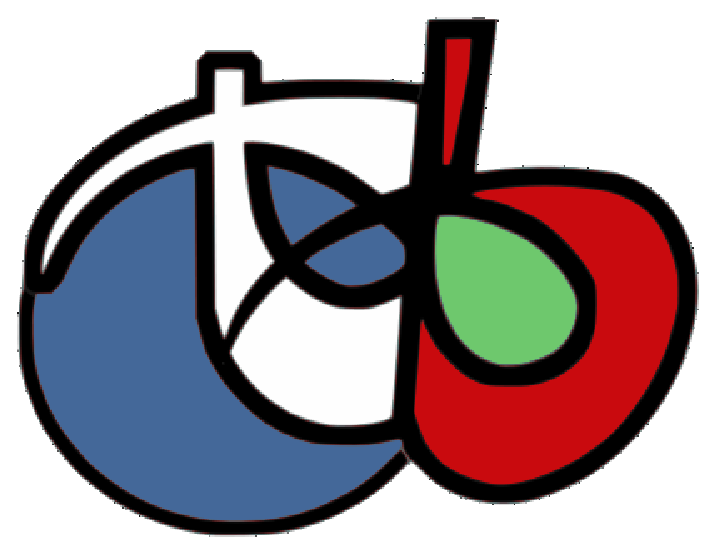
\includegraphics[width=0.5\textwidth]{logoVectoriel.eps}
\large
\begin{center}
\emph{The ORFEO Toolbox is not a black box.}\\
\end{center}
\hspace{8cm} Ch.D.
\normalsize
\end{minipage}



%%%%%%%%%%%%%%%%%%%%%%%%%%%%%%%%%%%%%%%%%%%%%%
%
% remove headings from the following material
\pagestyle{plain}
%
%%%%%%%%%%%%%%%%%%%%%%%%%%%%%%%%%%%%%%%%%%%%%%



%%\ifitkPrintedVersion
%% % We want this material to fit on two pages
\small

\chapter*{About the Cover}

Creating the cover image demonstrating the capabilities of the toolkit was a
challenging task.\footnote{The source code for the cover is available from
InsightDocuments/SoftwareGuide/Cover/Source/.} Given that the origins of ITK
are with the Visible Human Project it seemed appropriate to create an image
utilizing the VHP data sets, and it was decided to use the more recently
acquired Visible Woman dataset.  Both the RGB cryosections and the CT scans
were combined in the same scene.

\begin{description}

\item [Removing the Gel.]
The body of the Visible Woman was immersed in a block of gel during the
freezing process. This gel appears as a blue material in the cryogenic data.
To remove the gel, the joint histogram of RGB values was computed. This
resulted in an 3D image of $256\times256\times256$ pixels. The histogram
image was visualized in VolView.\footnote{VolView is a commercial product
from Kitware. It supports ITK plug-ins and is available as a free viewer or
may be licensed with advanced functionality. See
http://www.kitware.com/products/volview.html for information.} The cluster
corresponding to the statistical distribution of blue values was identified
visually, and a separating plane was manually defined in RGB space. The
equation of this plane was subsequently used to discriminate pixels in the
gel from pixels in the anatomical structures. The gel pixels were zeroed out
and the RGB values on the body were preserved.

\item[The Skin.]
The skin was easy to segment once the gel was removed. A simple region
growing algorithm was used requiring seed points in the region previously
occupied by the gel and then set to zero values. An anti-aliasing filter was
applied in order to generate an image of pixel type float where the surface
was represented by the zero set. This data set was exported to VTK where a
contouring filter was used to extract the surface and introduce it in the VTK
visualization pipeline.

\item[The Brain.]
The visible part of the brain represents the surface of the gray matter.  The
brain was segmented using the vector version of the confidence connected
image filter.  This filter implements a region growing algorithm that starts
from a set of seed points and adds neighboring pixels subject to a condition
of homogeneity.

The set of sparse points obtained from the region growing algorithm was
passed through a mathematical morphology dilation in order to close holes and
then through a binary median filter. The binary median filter has the
outstanding characteristic of being very simple in implementation by applying
a sophisticated effect on the image. Qualitatively it is equivalent to a
curvature flow evolution of the iso-contours. In fact the binary median
filter as implemented in ITK is equivalent to the majority filter that
belongs to the family of voting filters classified as a subset of the
\emph{Larger than Life} cellular automata. Finally, the volume resulting from
the median filter was passed through the anti-aliasing image filter. As
before, VTK was used to extract the surface.

\item[The Neck Musculature.]
The neck musculature was not perfectly segmented. Indeed, the resulting
surface is a fusion of muscles, blood vessels and other anatomical
structures. The segmentation was performed by applying the
VectorConfidenceConnectedImageFilter to the cryogenic dataset. Approximately
60 seed points were manually selected and then passed to the filter as
input. The binary mask produced by the filter was dilated with a mathematical
morphology filter and smoothed with the BinaryMedianImageFilter. The
AntiAliasBinaryImageFilter was used at the end to reduce the pixelization
effects prior to the extraction of the iso-surface with vtkContourFilter.

\item[The Skull.]
The skull was segmented from the CT data set and registered to the cryogenic
data. The segmentation was performed by simple thresholding, which was good
enough for the cover image. As a result, most of the bone structures are
actually fused together. This includes the jaw bone and the cervical
vertebrae.

\item[The Eye.] 
The eye is charged with symbolism in this image. This is due in part because
the motivation for the toolkit is the analysis of the Visible Human data,
and in part because the name of the toolkit is \emph{Insight}.

The first step in processing the eye was to extract a sub-image of
$60\times60\times60$ pixels centered around the eyeball from the RGB
cryogenic data set. This small volume was then processed with the vector
gradient anisotropic diffusion filter in order to increase the homogeneity of
the pixels in the eyeball.

The smoothed volume was segmented using the
VectorConfidenceConnectedImageFilter using 10 seed points. The resulting
binary mask was dilated with a mathematical morphology filter with a
structuring element of radius one, then smoothed with a binary mean image
filter (equivalent to majority voting cellular automata). Finally the mask
was processed with the AntiAliasBinaryImageFilter in order to generate a
float image with the eyeball contour embedded as a zero set.

\item[Visualization.]
The visualization of the segmentation was done by passing all the binary
masks through the AntiAliasBinaryImageFilter, generating iso-contours with
VTK filters, and then setting up a VTK Tcl script. The skin surface was
clipped using the vtkClipPolyDataFilter using the implicit function
vtkCylinder. The vtkWindowToImageFilter proved to be quite useful for
generating the final high resolution rendering of the scene ($3000\times3000$
pixels).

\item[Cosmetic Postprocessing.]
We have to confess that we used Adobe Photoshop to post-process the image. In
particular, the background of the image was adjusted using Photoshop's color
selection. The overall composition of the image with the cover text and
graphics was also performed using Photoshop.

\end{description}

\normalsize

%%\fi

\chapter*{Foreword}
\noindent


Beside the Pleiades (PHR) and Cosmo-Skymed (CSK) systems developments
forming ORFEO, the dual and bilateral system (France - Italy) for
Earth Observation, the ORFEO Accompaniment Program was set up, to
prepare, accompany and promote the use and the exploitation of the
images derived from these sensors.

The creation of a preparatory
program\footnote{http://smsc.cnes.fr/PLEIADES/A\_prog\_accomp.htm} is
needed because of:
\begin{itemize}
\item the new capabilities and performances of the ORFEO systems
  (optical and radar high resolution, access capability, data quality,
  possibility to acquire simultaneously in optic and radar),
\item the implied need of new methodological developments : new
  processing methods, or adaptation of existing methods,
\item the need to realise those new developments in very close
  cooperation with the final users for better integration of new
  products in their systems.

\end{itemize}

This program was initiated by CNES mid-2003 and will last until mid
2013.  It consists in two parts, between which it is necessary to keep
a strong interaction:
\begin{itemize}
\item A Thematic part,
\item A Methodological part.
\end{itemize}

The Thematic part covers a large range of applications (civil and
defence), and aims at specifying and validating value added products
and services required by end users. This part includes consideration
about products integration in the operational systems or processing
chains. It also includes a careful thought on intermediary structures
to be developed to help non-autonomous users. Lastly, this part aims
at raising future users awareness, through practical demonstrations
and validations.

The Methodological part objective is the definition and the
development of tools for the operational exploitation of the
submetric optic and radar images (tridimensional aspects, changes
detection, texture analysis, pattern matching, optic radar
complementarities). It is mainly based on R\&D studies and doctorate
and post-doctorate researches.

In this context, CNES\footnote{http://www.cnes.fr} decided to develop
the \emph{ORFEO ToolBox} (OTB), a set of algorithms encapsulated in a
software library. The goals of the OTB is to capitalise a methological
\textit{savoir faire} in order to adopt an incremental development
approach aiming to efficiently exploit the results obtained in the
frame of methodological R\&D studies.

All the developments are based on FLOSS (Free/Libre Open Source Software) or
existing CNES developments. OTB is distributed under the permissive open
source license Apache v2.0 - aka Apache Software License (ASL) v2.0:\\
\url{http://www.apache.org/licenses/LICENSE-2.0}

OTB is implemented in C++ and is mainly based on
ITK\footnote{http://www.itk.org} (Insight Toolkit).


%% L'environnement de l'OTB est mis en place par l'outil CMake\footnote{http://www.cmake.org},
%% permettant ainsi de g\'{e}rer les proc\'{e}dures de compilation, g\'{e}n\'{e}ration et d'installation et ce quelque sois la plate forme cible.

%% Dans un souci d'homog\'{e}n\'{e}isation, l'OTB est con\c{c}ue et d\'{e}velopp\'{e}e suivant la philosophie et les principes \'{e}dict\'{e}s
%% par la biblioth\`{e}que ITK (programmation g\'{e}n\'{e}rique, m\'{e}canisme des \emph{Object Factories}, \emph{Smart pointers}, exceptions, \emph{Multi-Threading}, etc...).
%% Ces principes sont pr\'{e}sent\'{e}s dans le paragraphe \emph{3.2 Essential System Concepts} du guide ITK \url{http://www.itk.org/ItkSoftwareGuide.pdf}

%% Enfin, la m\'{e}thodologie de d\'{e}veloppement appliqu\'{e}e s'appuie sur une approche it\'{e}rative bas\'{e}e sur la programmation agile :
%% le sch\'{e}ma de d\'{e}veloppement suit le cycle \'{e}dict\'{e}e par la m\'{e}thodolgie de l'eXtreme Programming (XP)\footnote{http://www.xprogramming.com}.



%% Ce document constitue le guide d'utilisation et de d\'{e}veloppement de l'OTB. La version la plus r\'{e}cente de ce document est accessible \`{a}
%% \url{http://smsc.cnes.fr/PLEIADES/Fr/A_prog_accomp.htm/OTB/otbSoftwareGuide.pdf}.





%%%%%%%%%%%%%%%%%%%%%%%%%%%%%%%%%%%%%%%%%%%%%%%%%%%%%%%%%
%
% Insert Table of Contents; List of Figures and Tables
%
%%%%%%%%%%%%%%%%%%%%%%%%%%%%%%%%%%%%%%%%%%%%%%%%%%%%%%%%%


%%%%%%%%%%%%%%%%%%%%%%%%%%%%%%%%%%%%%%%%%%%%%%
%
% enable headings from the following material
\pagestyle{normal}
%
%%%%%%%%%%%%%%%%%%%%%%%%%%%%%%%%%%%%%%%%%%%%%%
\small
\tableofcontents
\listoffigures
\listoftables
\normalsize




%%%%%%%%%%%%%%%%%%%%%%%%%%%%%%%%%%%%%%%%%
%
% Begin technical content
%
%%%%%%%%%%%%%%%%%%%%%%%%%%%%%%%%%%%%%%%%%

\mainmatter

\part{Introduction}\label{part:introduction}

\chapter{Welcome}
\label{chapter:Welcome}

Welcome to the \emph{ORFEO ToolBox (OTB) Software Guide}.

This document presents the essential concepts used in OTB. It will
guide you through the road of learning and using OTB. The Doxygen
documentation for the OTB application programming interface is
available on line.

\section{Organisation}
\label{sec:Organisation}

This guide is divided in three parts, each of which is further divided
into chapters.

La premi\`{e}re partie pr\'{e}sente l'OTB de fa\c{c}on g\'{e}n\'{e}rale, comment proc\'{e}der \`{a} son installation et sa g\'{e}n\'{e}ration sur votre machine. 
Cette partie pr\'{e}sente donc les principes de bases d'architecture et de compilation sur un syt\`{e}me, et comment compiler une application en C++.

La deuxi\`{e}me partie pr\'{e}sente l'OTB d'un point de vue \emph{utilisateur}. Elle se pr\'{e}sente sous forme d'exemples illutr\'{e}s.

La troisi\`{e}me partie pr\'{e}sente l'OTB d'un point de vue \emph{d\'{e}veloppeur}.
Cette partie explique comment cr\'{e}er vos propres classes, comment faire \'{e}voluer le produit.

\section{Se familiariser avec l'OTB}
\label{sec:CommentApprendreOTB}

Il y \`{a} deux cat\'{e}gories d'utilisateurs de l'OTB :
\begin{itemize}
        \item Les d\'{e}veloppeurs de classes, qui cr\'{e}ent des classes C++. 
        \item Les utilisateurs des classes existantes pour d\'{e}velopper et g\'{e}n\'{e}rer leurs propres applications.
\end{itemize}

Nous vous recommendons d'\'{e}tudier les exemples. Vous pourrez ainsi compiler et ex\'{e}cuter les exemples distribu\'{e}s 
avec le code source diponible dans le r\'{e}pertoire \code{OTB/Examples}. Lire le fichier \code{OTB/Examples/README.txt} 
d\'{e}crivant les diff\'{e}rents exemples founis dans les sous-r\'{e}pertoires.

Il y \`{a} de plus, un ensemble de tests suffisamment document\'{e}s et disponibles dans le r\'{e}pertoire \code{OTB/Testing/Code} qui vous 
montrent comment peuvent \^{e}tre utilis\'{e}es les classes dans l'OTB.

\section{Organisation du logiciel}
\label{sec:OrganisationLogiciel}

En cours ....

\section{T\'{e}l\'{e}charger l'OTB}
\label{sec:DownloadOTB}
 
\index{Downloading}

L'OTB peut \^{e}tre t\'{e}l\'{e}charg\'{e}e \`{a} l'adresse Internet 
\begin{center} 
  \url{http://www.cnes.fr/HTML/Download.php}
\end{center}

\subsection{T\'{e}l\'{e}charger le 'Package'}
\label{sec:DownloadingReleases}

\index{OTB!downloading release}

Avant de d\'{e}marrer, vous pouvez consulter le document \code{GettingStarted.txt}\footnote{http://www.cnes.fr/HTML/GettingStarted.txt}. 
Il vous donne un aper\c{c}u sur la proc\'{e}dure \`{a} suivre pour le t\'{e}l\'{e}chargement et l'installation.

Choisir le fichier compress\'{e} \code{.zip} ou \code{.tgz}. Le premier est plut\^{o}t destin\'{e} pour l'environnement \emph{Microsoft Windows}, 
le second pour les environnements \emph{unix} ou \emph{linux}.

Extraire le contenu du fichier compress\'{e} (avec \emph{unzip} ou \emph{gunzip}) dans le r\'{e}pertoire \code{OTB} 
pr\'{e}alablement cr\'{e}\'{e} sur votre syt\`{e}me.
Vous \^{e}tes alors pr\^{e}t \`{a} proc\'{e}der \`{a} la configuration et l'installation du produit, 
d\'{e}crite au chapitre \ref{sec:CMakeforOTB} \`{a} la page \pageref{sec:CMakeforOTB}.

\subsection{T\'{e}l\'{e}charger depuis SVN}
\label{sec:DownloadingFromSVN}

\index{OTB!SVN repository}



Le code source de l'OTB est accessible via un serveur \href{http://subversion.tigris.org/}{Subversion SVN} (rempla\c{c}ant du c\'{e}l\`{e}bre CVS)
 

Pour acc\'{e}der \`{a} l'OTB via SVN (sous UNIX et Cygwin), utilisez la commande suivante :
\begin{verbatim}
svn ......
\end{verbatim}

Ceci permet de t\'{e}l\'{e}charger le r\'{e}pertoire \code{OTB} contenant l'ensemble du code source de la biblioth\`{e}que \emph{OTB}.

Vous pouvez ensuite configurer et installer l'OTB sur votre syst\`{e}me en suivant les instructions d\'{e}crites 
au chapitre \ref{sec:CMakeforOTB} \`{a} la page \pageref{sec:CMakeforOTB})


\subsection{Arborescence du produit}
\label{sec:DirectoryStructure}

L'OTB est organis\'{e} en trois principaux composants : la biblioth\`{e}que OTB (r\'{e}pertoire \code{OTB}), 
les applications de l'OTB (r\'{e}pertoire \code{OTB-Applications}) et la documentation associ\'{e}e (r\'{e}pertoire \code{OTB-Documents}).

Le code source ainsi que les exemples se trouvent dans le r\'{e}pertoire \code{OTB}; la documentation, 
le tutorial et les proc\'{e}dures d'installation se trouvent dans le r\'{e}pertoire \code{OTB-Documents} ; 
les applications plus complexes (de plus haut niveau) se trouvent dans le r\'{e}pertoire \code{OTB-Applications}.


L'\code{OTB} contient les r\'{e}pertoires suivants :
\begin{itemize}
        \item \code{OTB/Code} --- contient globalement l'ensemble du code source de la biblioth\`{e}que OTB
        \item \code{OTB/Documentation} --- contient la documentation de la biblioth\`{e}que OTB, produite par Doxygen
        \item \code{OTB/Examples} --- contient un ensemble d'exemples, utilis\'{e}s notamment pour pr\'{e}senter le concept de l'OTB et 
        \'{e}galement utilis\'{e} pour illustrer le guide de l'OTB
        \item \code{OTB/Testing} --- contient un certain nombre de programmes, utilis\'{e}s pour tester et valider la biblioth\`{e}que OTB. 
        Ces tests sont lanc\'{e}s via le moniteur de test de CMake \emph{ctest}.
        \item \code{OTB/Utils} --- contient les codes sources des biblioth\`{e}ques utilis\'{e}es par l'OTB
\end{itemize}

Le r\'{e}pertoire \code{OTB/Code} (le coeur du logiciel) est structur\'{e} de la fa\c{c}on suivante :
\begin{itemize}
        \item \code{OTB/Code/Common} --- d\'{e}finitions de macro, typedefs, et toutes autres classes "factoris\'{e}es" utilis\'{e}es par les autres composants de l'OTB.
        \item \code{OTB/Code/IO} --- classes d'entr\'{e}es/sorties pour l'acc\`{e}s aux images (encapsulation de GDAL et de CAI)
        \item \code{OTB/Code/ChangeDetection} --- les classes de d\'{e}tections de changements
        \item \code{OTB/Code/FiterExtraction} --- les classes contenant les primitives et descripteurs impl\'{e}ment\'{e}s
        \item \code{OTB/Code/Learning} --- les classes d'apprentissage supervis\'{e} (utilisant SVM)
        \item \code{OTB/Code/Visu} --- les classes de visualisation et des IHM graphiques (utilisant VTK et FLTK)
\end{itemize}

Le r\'{e}pertoire \code{OTB-Documents} contient les r\'{e}pertoires suivants :
\begin{itemize}
        \item \code{OTB-Documents/Latex} --- fichiers \LaTeX{} utilis\'{e}s pour la production de documents.
        \item \code{OTB-Documents/SoftwareGuide} --- fichiers \LaTeX{} utilis\'{e}s pour g\'{e}n\'{e}rer ce guide. 
        Les exemples illustr\'{e}s dans ce guide sont g\'{e}n\'{e}r\'{e}s \`{a} partir des codes sources, contenus 
        dans le r�pertoire \code{OTB/Examples}, traduits en \LaTeX{}
\end{itemize}

La documentation \code{OTB-Documents} est disponible via SVN en utilisant la commande :
\begin{verbatim}
svn ....
\end{verbatim}


Le r�pertoire \code{OTB-Applications} contient les r\'{e}pertoires suivants :
\begin{itemize}
        \item \code{OTB-Applications/Chgts} --- application int\'{e}ractive de d\'{e}tection de changements, utilisant l'\code{OTB}
        \item \code{OTB-Applications/Viewer} --- outil de visualisation d'images
        \item \code{OTB-Applications/Utils} --- contient divers utilitaires comme par exemple un g\'{e}n\'{e}rateur de quick-looks, 
        un outil d'extraction de r\'{e}gions d'int\'{e}r\^{e}t, un outil d'affichage des m\'{e}ta-donn\'{e}es des images et 
        un outil de pseudo-ortho-rectification automatique d'images
\end{itemize}

Pour acc\'{e}der aux applications de l'OTB via SVN (sous UNIX et Cygwin), utilisez la commande suivante :
\begin{verbatim}
svn ......
\end{verbatim}


\subsection{Documentation}
\label{sec:Documentation}

Associ\'{e}e \`{a} ce document, il existe deux autres documentations :
\begin{description}
        \item[La Documentation Doxygen .] La documentation Doxygen est une documentation essentielle pour d\'{e}velopper avec l'OTB. 
        Sous format HTML, elle d\'{e}crit en d\'{e}tail chaque classes et m\'{e}thodes impl\'{e}ment\'{e}es dans l'OTB. 
        Elle est illustr\'{e}e par des diagrammes de collaboration et des diagrammes d'h\'{e}ritage. 
        Cette documentation tr\`{e}s dynamique poss\`{e}de des hyper-liens sur les autres classes et sur le code source.
        Cette docmentation est disponible \`{a} l'adresse \url{http://smsc.cnes.fr/PLEIADES/Fr/A_prog_accomp.htm/}.
	\item[Les fichiers \emph{Header}.] Chaque classe de l'OTB est impl\'{e}ment\'{e}e dans un fichier .h et dans un fichier 
	.cxx/.txx (.txx pour les classes g�n�riques (\emph{template}) )
\end{description}

\subsection{Data}
\label{sec:Data}

Les images utilis\'{e}es dans ce guide proviennent de ............. 


\setcounter{secnumdepth}{3}

\chapter{Compiling OTB from source}
\label{chapter:Installation}
\index{Installation}

There are two ways to install OTB library on your system: installing from a binary distribution or compiling from sources. 
You can find information about the installation of binary packages for OTB and Monteverdi in the OTB-Cookbook.
This chapter covers compilation of OTB library from source.

OTB has been developed and tested across different combinations of operating systems, compilers, and hardware platforms including Windows, Linux and Mac OSX.  It is known to work with the following compilers in 32/64 bit:
\begin{itemize}
\item Visual Studio 2015 on Windows
\item GCC 4.x on GNU/Linux
\item AppleClang on MacOSX (10.8 or higher)
\end{itemize}

\index{CMake}
The challenge of supporting OTB across platforms has been solved through the use of CMake, a cross-platform, open-source
build system. CMake is used to control the software compilation process using simple platform and compiler independent
configuration files.  CMake generates native makefiles and workspaces that can be used in the compiler environment of
your choice. CMake is quite sophisticated: it supports complex environments requiring system configuration, compiler
feature testing, and code generation.

CMake supports several generators to produce the compilation scripts, dependending on the platform and compiler. It can use :
\begin{itemize}
\item Makefiles for Unix systems
\item Visual Studio workspaces for Windows
\item NMake Makefiles for Windows
\item Ninja scripts
\item and many more ...
\end{itemize}
The information used by CMake is provided by \code{CMakeLists.txt} files that
are present in every directory of the OTB source tree. These files contain information that the user provides to CMake
at configuration time. Typical information includes paths to utilities in the system and the selection of software
options specified by the user.

There are (at least) two ways to use CMake :
\begin{itemize}
\item Using the command \texttt{ccmake} (on Unix) or \texttt{cmake-gui} (on Windows): 
it provides an interactive mode in which you iteratively select
options and configure according to these options. The iteration
proceeds until no more options remain to be selected. At this point, a
generation step produces the appropriate build files for your
configuration. This is the easiest way to start.
\item Using the command \texttt{cmake} : it is a non-interactive polyvalent tool designed for scripting. It can run both \textit{configure} and \textit{generate} steps.
\end{itemize}

As shown in figure \ref{fig:CMakeGUI}, CMake has a different interfaces according to your system.
Refer to section~\ref{sec:compiling-linux} for Linux and Mac~OS~X build instructions
and \ref{sec:compiling-windows} for Windows.

\begin{figure}[tpb]
\centering
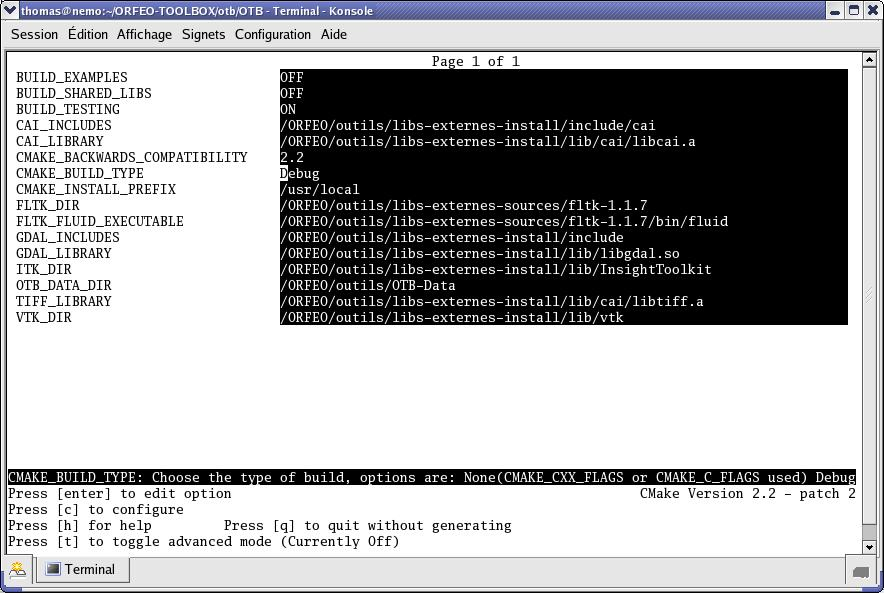
\includegraphics[width=0.8\textwidth]{ccmakeScreenShot.eps}
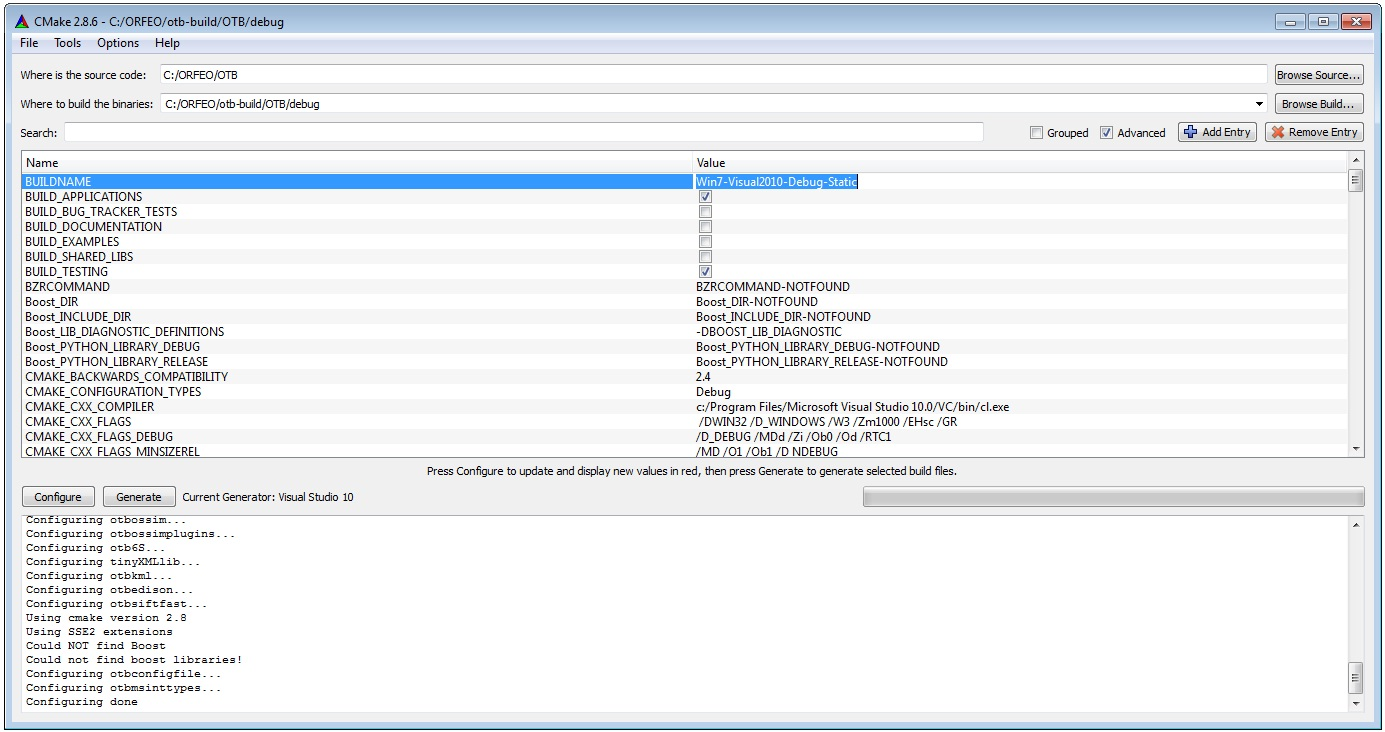
\includegraphics[width=0.8\textwidth]{CMakeSetupScreenShot.eps}
\itkcaption[Cmake user interface]{CMake interface. Top) \texttt{ccmake}, the UNIX
version based on \texttt{curses}. Bottom) \texttt{CMakeSetup}, the MS-Windows
version based on MFC.}
\label{fig:CMakeGUI}
\end{figure}

For more information on CMake, check :
\begin{center}
\url{http://www.cmake.org}
\end{center}

\index{Dependencies}
OTB depends on a number of external libraries.
Some are mandatory, meaning that OTB cannot be compiled without them, while others are optional and can be activated or
not during the build process.
See table \ref{tab:otb-dependencies} for the full list of dependencies.
\begin{center}
\begin{tiny}
\begin{table}[!htbp]
\begin{tabular}{|p{0.15\textwidth}|p{0.45\textwidth}|p{0.1\textwidth}|p{0.1\textwidth}|}
\hline
\textbf{Library} & \textbf{Web site} & \textbf{Mandatory} & \textbf{Minimum version} \\
\hline
\textbf{ITK} & \url{http://www.itk.org} & yes & 4.6.0 \\
\hline
\textbf{GDAL} & \url{http://www.gdal.org} & yes & 1.10 \\
\hline
\textbf{OSSIM} & \url{http://www.ossim.org} & yes & 1.8.20-3 \\
\hline
\textbf{Curl} & \url{http://www.curl.haxx.se} & no  & - \\
\hline
\textbf{FFTW} & \url{http://www.fftw.org} & no  & - \\
\hline
\textbf{libgeotiff} & \url{http://trac.osgeo.org/geotiff/} & yes & - \\
\hline
\textbf{OpenJPEG} & \url{http://code.google.com/p/openjpeg/} & no & - \\
\hline
\textbf{boost} & \url{http://www.boost.org} & yes & - \\
\hline
\textbf{openthreads} & \url{http://www.openscenegraph.org} & yes & - \\
\hline
\textbf{Mapnik} & \url{http://www.mapnik.org} & no  & - \\
\hline
\textbf{tinyXML} & \url{http://www.grinninglizard.com/tinyxml} & yes & - \\
\hline
\textbf{6S} & \url{http://6s.ltdri.org} & no & - \\
\hline
\textbf{SiftFast} & \url{http://libsift.sourceforge.net} & no  & - \\
\hline
\textbf{MuParser} & \url{http://www.muparser.sourceforge.net} & no  & - \\
\hline
\textbf{MuParserX} & \url{http://muparserx.beltoforion.de} & no  & 3.0.5 \\
\hline
\textbf{libSVM} & \url{http://www.csie.ntu.edu.tw/~cjlin/libsvm} & no  & 2.0 \\
\hline
\textbf{Qt} & \url{http://qt-project.org/} & no  & 4 \\
\hline
\textbf{OpenCV} & \url{http://opencv.org} & no  & 2 \\
\hline
\end{tabular}
\caption{External libraries used in OTB.}
\label{tab:otb-dependencies}
\end{table}
\end{tiny}
\end{center}

\section{Linux and Mac OS X}
\label{sec:compiling-linux}

\subsection{Setting up the build environment}

The first thing to do is to create a directory for working with OTB.
This guide will use \texttt{$\sim$/OTB} but you are free to choose something else.
In this directory, there will be three locations:
\begin{itemize}
\item \texttt{$\sim$/OTB/otb} for the source file obtained from the git repository
\item \texttt{$\sim$/OTB/build} for the intermediate build objects, CMake specific files, libraries and binaries.
\item \texttt{$\sim$/OTB/install}, the installation directory for OTB once it is built.
A system location (\texttt{/usr/local} for example) can also be used, but installing locally is more flexible and does
not require root access.
\end{itemize}
To setup this structure, the following commands can be used:
\begin{verbatim}
$ mkdir ~/OTB
$ cd ~/OTB
$ git clone https://git@git.orfeo-toolbox.org/git/otb.git
$ mkdir build
$ mkdir install
\end{verbatim}

The OTB project uses a git branching model where \texttt{develop} is the current development version.
It contains the latest patches and represents the work in progress towards the next release.
For more information on OTB and git, including how to decide which branch to want to compile, please see the
OTB wiki page at \url{http://wiki.orfeo-toolbox.org/index.php/Git}.

Checkout the relevant branch now:
\begin{verbatim}
$ cd ~/OTB/otb
$ git checkout develop
\end{verbatim}

Now you must decide which build method you will use.
There are two ways of compiling OTB from sources, depending on how you want to manage dependencies.
Both methods rely on CMake.
\begin{itemize}
\item SuperBuild (go to section~\ref{sec:installation-linux-superbuild}). All OTB dependencies are automatically downloaded and compiled.
This method is the easiest to use and provides a complete OTB with minimal effort.
\item Normal build (go to section~\ref{sec:installation-linux-normalbuild}). OTB dependencies must already be compiled and available on your system.
This method requires more work but provides more flexibility.
\end{itemize}
If you do not know which method to use and just want to compile OTB with all its modules, use SuperBuild.

\begin{center}
\begin{tiny}
\begin{table}[!htbp]
\begin{tabular}{p{0.35\textwidth}p{0.65\textwidth}}
\hline
\textbf{CMake variable} & \textbf{Value} \\
\hline
\texttt{CMAKE\_INSTALL\_PREFIX}         & Installation directory, target for \texttt{make install} \\
\texttt{BUILD\_EXAMPLES}                & Activate compilation of OTB examples \\
\texttt{BUILD\_TESTING}                 & Activate compilation of the tests \\
\texttt{OTB\_BUILD\_DEFAULT\_MODULES}   & Activate all usual modules, required to build the examples \\
\texttt{OTB\_USE\_\textit{XXX}}         & Activate module \textit{XXX} \\
\texttt{OTBGroup\_\textit{XXX}}         & Enable modules in the group \textit{XXX} \\
\texttt{OTB\_DATA\_ROOT}                & otb-data repository \\
\texttt{OTB\_WRAP\_PYTHON}              & Enable Python wrapper \\
\texttt{OTB\_WRAP\_JAVA}                & Enable Java wrapper \\

\hline
\multicolumn{2}{l}{\small \textbf{SuperBuild only}} \\ 
\texttt{DOWNLOAD\_LOCATION}             & Location to download dependencies \\
\texttt{USE\_SYSTEM\_\textit{XXX}}      & Use the system's \textit{XXX} library \\

\hline
\end{tabular}
\caption{Important CMake configuration variables in OTB}
\label{tab:installation-cmake-variables}
\end{table}
\end{tiny}
\end{center}

\subsection{SuperBuild: Build OTB and all dependencies}
\label{sec:installation-linux-superbuild}

The SuperBuild is a way of compiling dependencies to a project just before you build the project. Thanks to CMake and
its ExternalProject module, it is possible to download a source archive, configure and compile it when building
the main project. This feature has been used in other CMake-based projects (ITK, Slicer, ParaView,...).
In OTB, the SuperBuild is implemented with no impact on the library sources : the sources for SuperBuild are located in
the 'OTB/SuperBuild' subdirectory. It is made of CMake scripts and source patches that allow to compile all the
dependencies necessary for OTB. Once all the dependencies are compiled and installed, the OTB library is built using
those dependencies.

OTB's compilation is customized by specifying configuration variables.
The most important configuration variables are shown in table~\ref{tab:installation-cmake-variables}.
The simplest way to provide configuration variables is via the command line \texttt{-D} option:
\begin{verbatim}
$ cd ~/OTB/build
$ cmake -D CMAKE_INSTALL_PREFIX=~/OTB/install ../otb/SuperBuild
\end{verbatim}
A pre-load script can also be used with the \texttt{-C} options (see
\url{https://cmake.org/cmake/help/v3.4/manual/cmake.1.html#options}).
Another option is to set variables manually with \texttt{cmake-gui} or \texttt{ccmake}.

Please note that the \texttt{CMAKE\_INSTALL\_PREFIX} variable is important
because the SuperBuild will install some targets during the compilation step.
Therefore this directory will be used even if you don't use make install target.
In fact there is no make install target for the SuperBuild.

By default, SuperBuild will not use any of libraries installed on system. All \texttt{USE\_SYSTEM\_\textit{XXX}} are
are set to FALSE. This is our recommended way of using SuperBuild. You are however free to use a system library
if you want!. You must be very much aware of dependencies of those libraries you use from system. For example,
if libjpeg is not used from superbuild using \texttt{USE\_SYSTEM\_JPEG=TRUE} then you should not use zlib from superbuild
because zlib is a dependency of libjpeg. Here SuperBuild will not automagically set \texttt{USE\_SYSTEM\_ZLIB=FALSE}.
You must do it yourself. The example of libjpeg - zlib dependency chain is so simple.
Imagine the same case for GDAL which depends on zlib, libjpeg, libtiff(with big tiff support), geotiff,
sqlite, curl, geos, libkml, openjpeg. This is one of the reasons we recommend to use SuperBuild exclusively or not.

All dependencies are configured and built in a way that help us to get an efficient build OTB.
So we enable geotiff (with proj4 support), openjpeg, geos in GDAL build.

It is also important to note that SuperBuild is tested daily on all three platforms that makes us clear that
there is no issue with new changes in OTB and its dependencies. It simply works!

(see table~\ref{tab:installation-cmake-variables}).

SuperBuild downloads dependencies into the \texttt{DOWNLOAD\_LOCATION} directory, which will be
\texttt{$\sim$/OTB/build/Downloads} in our example.
Dependencies can be downloaded manually into this directory before the compilation step.
This can be usefull if you wish to bypass a proxy, intend to compile OTB without an internet conection, or other network
constraint. You can find an archive with sources of all our dependencies on the Orfeo ToolBox website (pick the 'SuperBuild-archives' corresponding to the OTB version you want to build) :
\begin{center}
\url{https://www.orfeo-toolbox.org/packages}
\end{center}

You are now ready to compile OTB!
Simply use the make command (other targets can be generated with CMake's \texttt{-G} option):
\begin{verbatim}
$ cd ~/OTB/build
$ make
\end{verbatim}

Applications will be located in the \texttt{bin/} directory, for example:
\begin{verbatim}
./OTB/build/bin/otbcli_ExtractROI
\end{verbatim}
will launch the command line version of the \textbf{ExtractROI} application,
while:
\begin{verbatim}
./OTB/build/bin/otbgui_ExtractROI
\end{verbatim}
will launch the graphical version.

We recommend adding OTB build directory to your PATH for easy access:
\begin{verbatim}
export PATH=$PATH:~/OTB/build/OTB/build/bin
\end{verbatim}

Monteverdi is also compiled by the SuperBuild (as long as you activate it with
ENABLE\_MONTEVERDI). To use OTB applications from within Monteverdi you will need
to define the OTB\_APPLICATION\_PATH environment variable.
\begin{verbatim}
export OTB_APPLICATION_PATH=~/OTB/build/OTB/build/lib/otb/applications
monteverdi
\end{verbatim}

A wiki page detailing the status of SuperBuild on various platforms is also available here:
\url{http://wiki.orfeo-toolbox.org/index.php/SuperBuild}.

\subsection{Normal build: Build only OTB}
\label{sec:installation-linux-normalbuild}

Once all OTB dependencies are availables on your system, use CMake to generate a Makefile:
\begin{verbatim}
$ cd ~/OTB/build
$ cmake -C configuration.cmake ../otb
\end{verbatim}
The script \texttt{configuration.cmake} needs to contain dependencies location if CMake cannot find them automatically.
This can be done with the \texttt{\textit{XXX}\_DIR} variables containing the directories which contain the
FindXXX.cmake scripts, or with the \texttt{\textit{XXX}\_INCLUDEDIR} and \texttt{\textit{XXX}\_LIBRARY} variables.

Additionally, decide which module you wish to enable, together with tests and examples.
Refer to table~\ref{tab:installation-cmake-variables} for the list of CMake variables.

Since OTB is modularized, it is possible to only build some modules instead of the whole set. 
To deactivate a module (and the ones that depend on it) switch off the CMake variable OTB\_BUILD\_DEFAULT\_MODULES,
configure, and then switch off each \texttt{Module\_module\_name} variable.
To provide an overview on how things work, the option \texttt{COMPONENTS} of the CMake command find\_package is used in
order to only load the requested modules.
This module-specific list prevent CMake from performing a blind search; it is also a convienent way to monitor the
dependencies of each module.
\begin{verbatim}
find_package(OTB COMPONENTS OTBCommon OTBTransform [...])
\end{verbatim} 

Some of the OTB capabilities are considered as optional, and you can deactivate the related modules thanks to a set of
CMake variables starting with \texttt{OTB\_USE\_\textit{XXX}}.
Table~\ref{tab:optional} shows which modules are associated to these variables. It is very important to notice that
these variable override the variable OTB\_BUILD\_DEFAULT\_MODULES.

You are now ready to compile OTB!
Simply use the make command (other targets can be generated with CMake's \texttt{-G} option):
\begin{verbatim}
$ make
\end{verbatim}

The installation target will copy the binaries and libraries to the installation location:
\begin{verbatim}
$ make install
\end{verbatim}

\begin{center}
\begin{tiny}
\begin{table}[!htbp]
\begin{tabular}{|l|l|p{0.52\textwidth}|}
\hline
\textbf{CMake variable} & \textbf{3rd party module} & \textbf{Modules depending on it} \\
\hline
\textbf{OTB\_USE\_LIBKML} & OTBlibkml & OTBKMZWriter OTBIOKML OTBAppKMZ \\
\hline
\textbf{OTB\_USE\_QT4} & OTBQt4 & OTBQtWidget \\
\hline
\textbf{OTB\_USE\_OPENCV} & OTBOpenCV & \\
\hline
\textbf{OTB\_USE\_MUPARSERX} & OTBMuParserX & OTBMathParserX OTBAppMathParserX \\
\hline
\textbf{OTB\_USE\_OPENJPEG} & OTBOpenJPEG & OTBIOJPEG2000 \\
\hline
\textbf{OTB\_USE\_CURL} & OTBCurl & \\
\hline
\textbf{OTB\_USE\_MUPARSER} & OTBMuParser & OTBMathParser OTBDempsterShafer OTBAppClassification OTBAppMathParser OTBAppStereo OTBAppProjection OTBAppSegmentation OTBAppClassification OTBRoadExtraction OTBRCC8 OTBCCOBIA OTBAppSegmentation OTBMeanShift OTBAppSegmentation OTBMeanShift OTBAppSegmentation \\
\hline
\textbf{OTB\_USE\_LIBSVM} & OTBLibSVM & OTBSVMLearning \\
\hline
\textbf{OTB\_USE\_MAPNIK} & OTBMapnik & OTBVectorDataRendering \\
\hline
\textbf{OTB\_USE\_6S} & OTB6S & OTBOpticalCalibration OTBAppOpticalCalibration OTBSimulation \\
\hline
\textbf{OTB\_USE\_SIFTFAST} & OTBSiftFast & \\
\hline
\end{tabular}
\caption{Third parties and related modules.}
\label{tab:optional}
\end{table}
\end{tiny}
\end{center}

\section{Windows}
\label{sec:compiling-windows}

Everything that is needed for OTB development on Windows, including compiling from source, is covered in details on the OTB wiki at:
\begin{center}
\url{http://wiki.orfeo-toolbox.org/index.php/OTB_development_on_Windows}
\end{center}

\section{Known issues}
\label{sec:knownissues}

\begin{itemize}
\item  openjpeg/ITK 
\end{itemize}

It is important to know that the OpenJpeg library doesn't support name mangling since version 2.0. 
As a consequence, if other libraries linked by your project already contain OpenJpeg, there may be a symbol conflict at run-time. 
For instance, this was observed with OTB build on a recent ITK version (ver. 4). 
The ITK library already had a version of OpenJpeg in libitkopenjpeg-*.so, which contained the OpenJpeg symbols un-wrapped.
These symbols were also loaded by the GDAL driver but only the first ones were used, which caused a crash. 

Hopefully, thanks to the modular architecture of ITK, the library libitkopenjpeg-*.so is not imported anymore inside OTB.
However the OpenJPEG headers may be present in ITK include directory. As the current architecture doesn't allow to tune 
include order between modules, the OpenJPEG header from ITK can be included before your own OpenJPEG install. There are
two ways to avoid this situation :
\begin{itemize}
\item Use an ITK without GDCM nor ITKReview (only these modules depend on OpenJPEG)
\item Hide the header openjpeg.h in the ITK include directory.
\end{itemize}

More information can be found here : \url{http://wiki.orfeo-toolbox.org/index.php/JPEG2000_with_GDAL_OpenJpeg_plugin}

\begin{itemize}
\item  libkml / Ubuntu 12.04 
\end{itemize}

Another issue is related to the official package of libkml under Ubuntu 12.4.
Until this problem is addressed, users of this plateform should disable the option OTB\_USE\_KML, so that OTB won't be built with this third-party.


\chapter{System Overview}
\label{chapter:SystemOverview}

The purpose of this chapter is to provide you with an overview of the
\emph{ORFEO Toolbox} system. We recommend that you read this chapter to
gain an appreciation for the breadth and area of application of
OTB. In this chapter, we will make reference either to \emph{OTB
  features} or \emph{ITK features} without distinction. Bear in mind
that OTB uses ITK as its core element, so all the fundamental elements
of OTB come from ITK. OTB extends the functionalities of ITK for the
remote sensing image processing comunity. We benefit from the Open
Source development approach chosen for ITK, which allows us to provide
an impressive set of functionalities with much lesser effort than it
would have been the case in a closed source universe!

\section{System Organization}
\label{sec:SystemOrganization}

The ORFEO Toolbox consists of several subsystems. A brief
description of these subsystems follows. Later sections in this chapter---and
in some cases additional chapters---cover these concepts in more detail. (Note:
in the previous chapter two other modules---\code{OTB-Documents} and
\code{OTB-Applications} were briefly described.)

\begin{description}
	\item[Essential System Concepts.] Like any software system, OTB is
        built around some core design concepts. OTB uses those of
        ITK. Some of the more important
        concepts include generic programming, smart pointers for memory
        management, object factories for adaptable object instantiation,
        event management using the command/observer design paradigm, and
        multithreading support.

	\item[Numerics] OTB, as ITK uses VXL's VNL numerics libraries. These are
        easy-to-use C++ wrappers around the Netlib Fortran numerical 
        analysis routines (\url{http://www.netlib.org}).

	\item[Data Representation and Access.]  Two principal classes
        are used to represent data: the \doxygen{otb}{Image} and
        \doxygen{itk}{Mesh} classes.  In addition, various types of
        iterators and containers are used in ITK to hold and traverse
        the data. Other important but less popular classes are also
        used to represent data such as histograms.

	\item[ITK's Data Processing Pipeline.]  The data representation
	classes (known as \emph{data objects}) are operated on by
	\emph{filters} that in turn may be organized into data flow
	\emph{pipelines}. These pipelines maintain state and therefore
	execute only when necessary.  They also support
	multi-threading, and are streaming capable (i.e., can operate
	on pieces of data to minimize the memory footprint).

        \item[IO Framework.] Associated with the data processing
        pipeline are \emph{sources}, filters that initiate the
        pipeline, and \emph{mappers}, filters that terminate the
        pipeline.  The standard examples of sources and mappers are
        \emph{readers} and \emph{writers} respectively.  Readers
        input data (typically from a file), and writers output data
        from the pipeline. \emph{Viewers} are another example of mappers.

	\item[Spatial Objects.] Geometric shapes are represented in
        OTB using the ITK spatial object hierarchy.  These classes are
        intended to support modeling of anatomical structures in
        ITK. OTB uses them in order to model cartographic elements. Using a
        common basic interface, the spatial objects are capable of
        representing regions of space in a variety of different
        ways. For example: mesh structures, image masks, and implicit
        equations may be used as the underlying representation scheme.
        Spatial objects are a natural data structure for communicating
        the results of segmentation methods and for introducing
        geometrical priors in both segmentation and registration
        methods.

	\item[ITK's Registration Framework.] A flexible framework for
        registration supports four different types of registration:
        image registration, multiresolution registration, PDE-based
        registration, and FEM (finite element method) registration.

	\item[FEM Framework.] ITK includes a subsystem for solving general
        FEM problems, in particular non-rigid registration. The FEM package
        includes mesh definition (nodes and elements), loads, and boundary
        conditions.

	\item[Level Set Framework.] The level set framework is a set of
        classes for creating filters to solve partial differential equations
        on images using an iterative, finite difference update scheme. The
        level set framework consists of finite difference solvers including a
        sparse level set solver, a generic level set segmentation filter, and
        several specific subclasses including threshold, Canny, and Laplacian
        based methods.

	\item[Wrapping.] ITK uses a unique, powerful system for
	producing interfaces (i.e., ``wrappers'') to interpreted
	languages such as Tcl and Python. The GCC\_XML tool is used to
	produce an XML description of arbitrarily complex C++ code;
	CSWIG is then used to transform the XML description into
	wrappers using the \href{http://www.swig.org/}{SWIG}
	package. OTB does not use this system at present.

%% 	\item[Auxiliary / Utilities] Several auxiliary subsystems are 
%%         available to supplement other classes in the system. For example,
%%         calculators are classes that perform specialized operations in
%%         support of filters (e.g., MeanCalculator computes the mean of a
%%         sample). Other utilities include GDAL format file
%%         support, png, zlib, FLTK / Qt image viewers, and interfaces to the
%%         Visualization Toolkit (VTK) system.
        
\end{description}


\section{Essential System Concepts}
\label{sec:EssentialSystemConcepts}

This section describes some of the core concepts and implementation features
found in ITK and therefore also in OTB.

\subsection{Generic Programming}
\label{sec:GenericProgramming}

\index{generic programming}
\index{template}

Generic programming is a method of organizing libraries consisting of
generic---or reusable---software components \cite{Musser1996}. The idea is to
make software that is capable of ``plugging together'' in an efficient,
adaptable manner. The essential ideas of generic programming are
\emph{containers} to hold data, \emph{iterators} to access the data, and 
\emph{generic algorithms} that use containers and iterators to create 
efficient, fundamental algorithms such as sorting. Generic programming is
implemented in C++ with the \emph{template} programming mechanism and the 
use of the STL Standard Template Library \cite{Austern1999}.

C++ templating is a programming technique allowing users to write software in
terms of one or more unknown types \code{T}. To create executable code, the
user of the software must specify all types \code{T} (known as \emph{template
instantiation}) and successfully process the code with the compiler. The
\code{T} may be a native type such as
\code{float} or \code{int}, or \code{T} may be a user-defined type (e.g.,
\code{class}). At compile-time, the compiler makes sure that the templated 
types are compatible with the instantiated code and that the types are
supported by the necessary methods and operators.

ITK uses the techniques of generic programming in its implementation. The
advantage of this approach is that an almost unlimited variety of data types
are supported simply by defining the appropriate template types. For example,
in OTB it is possible to create images consisting of almost any type of
pixel. In addition, the type resolution is performed at compile-time, so the
compiler can optimize the code to deliver maximal performance. The
disadvantage of generic programming is that many compilers still do not
support these advanced concepts and cannot compile OTB. And even if they do,
they may produce completely undecipherable error messages due to even the
simplest syntax errors. If you are not familiar with templated code and
generic programming, we recommend the two books cited above.

\subsection{Include Files and Class Definitions}
\label{sec:IncludeFiles}

In ITK and OTB classes are defined by a maximum of two files: a header \code{.h} file
and an implementation file---\code{.cxx} if a non-templated class, and a
\code{.txx} if a templated class.
The header files contain class declarations
and formatted comments that are used by the Doxygen documentation
system to automatically produce HTML manual pages.

In addition to class headers, there are a few other important header files.
\begin{description}
        \item[\code{itkMacro.h}] is found in the
        \code{Utilities/ITK/Code/Common} directory
        and defines standard system-wide macros (such as \code{Set/Get},
        constants, and other parameters).

        \item[\code{itkNumericTraits.h}] is found in the \code{Utilities/ITK/Code/Common}
        directory and defines numeric characteristics for native types such
        as its maximum and minimum possible values.

        \item[\code{itkWin32Header.h}] is found in the \code{Utilities/ITK/Code/Common}
        and is used to define operating system parameters to control
        the compilation process.
\end{description}

\subsection{Object Factories}
\label{sec:ObjectFactories}

\index{object factory}
\index{factory}

Most classes in OTB are instantiated through an \emph{object factory}
mechanism. That is, rather than using the standard C++ class constructor and
destructor, instances of an OTB class are created with the static class
\code{New()} method. In fact, the constructor and destructor are
\code{protected:} so it is generally not possible to construct an OTB
instance on the heap. (Note: this behavior pertains to classes that are
derived from \doxygen{itk}{LightObject}. In some cases the need for speed or
reduced memory footprint dictates that a class not be derived from
LightObject and in this case instances may be created on the heap. An
example of such a class is \doxygen{itk}{EventObject}.)

The object factory enables users to control run-time instantiation of classes
by registering one or more factories with \doxygen{itk}{ObjectFactoryBase}. These
registered factories support the method \code{CreateInstance(classname)}
which takes as input the name of a class to create. The factory can choose to
create the class based on a number of factors including the computer system
configuration and environment variables. For example, in a particular
application an OTB user may wish to deploy their own class implemented using
specialized image processing hardware (i.e., to realize a performance
gain). By using the object factory mechanism, it is possible at run-time to
replace the creation of a particular OTB filter with such a custom class. (Of
course, the class must provide the exact same API as the one it is
replacing.) To do this, the user compiles her class (using the same compiler,
build options, etc.) and inserts the object code into a shared library or
DLL. The library is then placed in a directory referred to by the
\code{OTB\_AUTOLOAD\_PATH} environment variable. On instantiation, the object
factory will locate the library, determine that it can create a class of a
particular name with the factory, and use the factory to create the
instance. (Note: if the \code{CreateInstance()} method cannot find a factory
that can create the named class, then the instantiation of the class falls
back to the usual constructor.)

In practice object factories are used mainly (and generally transparently) by
the OTB input/output (IO) classes. For most users the greatest impact is on
the use of the \code{New()} method to create a class. Generally the
\code{New()} method is declared and implemented via the macro
\code{itkNewMacro()} found in \code{Utilities/ITK/Common/itkMacro.h}.


\subsection{Smart Pointers and Memory Management}
\label{sec:SmartPointers}

\index{smart pointer}

By their nature object-oriented systems represent and operate on data through
a variety of object types, or classes. When a particular class is
instantiated to produce an instance of that class, memory allocation occurs
so that the instance can store data attribute values and method pointers
(i.e., the vtable). This object may then be referenced by other classes or
data structures during normal operation of the program. Typically during
program execution all references to the instance may disappear at which point
the instance must be deleted to recover memory resources. Knowing when to
delete an instance, however, is difficult. Deleting the instance too soon
results in program crashes; deleting it too late and memory leaks (or
excessive memory consumption) will occur. This process of allocating and
releasing memory is known as memory management.

In ITK, memory management is implemented through reference counting. This
compares to another popular approach---garbage collection---used
\index{garbage collection} by many
systems including Java. In reference counting, a count of the number of
references to each instance is kept. When the reference goes to zero, the
object destroys itself. In garbage collection, a background process sweeps
the system identifying instances no longer referenced in the system and
deletes them. The problem with garbage collection is that the actual point in
time at which memory is deleted is variable. This is unacceptable when an
object size may be gigantic (think of a large 3D volume gigabytes in
size). Reference counting deletes memory immediately (once all references to
an object disappear).

Reference counting is implemented through a \code{Register()}/\code{Delete()}
member function interface.  All instances of an OTB object have a
\code{Register()} method invoked on them by any other object that references
an them. The \code{Register()} method increments the instances' reference
count. When the reference to the instance disappears, a \code{Delete()}
method is invoked on the instance that decrements the reference count---this
is equivalent to an \code{UnRegister()} method. When the reference count
returns to zero, the instance is destroyed.

This protocol is greatly simplified by using a helper class called a
\doxygen{itk}{SmartPointer}. The smart pointer acts like a regular pointer
(e.g. supports operators \code{->} and \code{*}) but automagically performs a
\code{Register()} when referring to an instance, and an \code{UnRegister()}
when it no longer points to the instance.  Unlike most other instances in
OTB, SmartPointers can be allocated on the program stack, and are
automatically deleted when the scope that the SmartPointer was created
is closed. As a result, you should \emph{rarely if ever call Register() or
Delete()} in OTB. For example:

\small
\begin{verbatim}
  MyRegistrationFunction()
    { <----- Start of scope

    // here an interpolator is created and associated to the
    // SmartPointer "interp".
    InterpolatorType::Pointer interp = InterpolatorType::New();

    } <------ End of scope
\end{verbatim}
\normalsize

In this example, reference counted objects are created (with the \code{New()}
method) with a reference count of one. Assignment to the SmartPointer
\code{interp} does not change the reference count. At the end of scope,
\code{interp} is destroyed, the reference count of the actual interpolator
object (referred to by \code{interp}) is decremented, and if it reaches zero,
then the interpolator is also destroyed.

Note that in ITK SmartPointers are always used to refer to instances of
classes derived from \doxygen{itk}{LightObject}. Method invocations and function
calls often return ``real'' pointers to instances, but they are immediately
assigned to a SmartPointer. Raw pointers are used for non-LightObject classes when
the need for speed and/or memory demands a smaller, faster class.


\subsection{Error Handling and Exceptions}
\label{sec:ErrorHandling}

\index{exceptions}
\index{error handling}

In general, OTB uses exception handling to manage errors during program
execution. Exception handling is a standard part of the C++ language and
generally takes the form as illustrated below:
\small
\begin{verbatim}
  try
    {
    //...try executing some code here...
    }
  catch ( itk::ExceptionObject exp )
    {
    //...if an exception is thrown catch it here
    }
\end{verbatim}
\normalsize

where a particular class may throw an exceptions as demonstrated below (this
code snippet is taken from \doxygen{itk}{ByteSwapper}:
\small
\begin{verbatim}
  switch ( sizeof(T) )
    {
    //non-error cases go here followed by error case  
    default:  
      ByteSwapperError e(__FILE__, __LINE__);
      e.SetLocation("SwapBE");
      e.SetDescription("Cannot swap number of bytes requested");
      throw e;
    }
\end{verbatim}
\normalsize

Note that \doxygen{itk}{ByteSwapperError} is a subclass of
\doxygen{itk}{ExceptionObject}. (In fact in OTB all exceptions should be derived
from \code{itk::ExceptionObject}.) In this example a special constructor and C++
preprocessor variables \code{\_\_FILE\_\_} and \code{\_\_LINE\_\_} are used to instantiate
the exception object and provide additional information to the user. You can
choose to catch a particular exception and hence a specific OTB error, or you
can trap \emph{any} OTB exception by catching ExceptionObject.


\subsection{Event Handling}
\label{sec:EventHandling}

\index{event handling}
\index{Command/Observer design pattern}
\index{itk::Command}
\index{ProgressEvent()}
\index{InvokeEvent()}

Event handling in OTB is implemented using the Subject/Observer design
pattern \cite{Gamma1995} (sometimes referred to as the Command/Observer
design pattern). In this approach, objects indicate that they are watching
for a particular event---invoked by a particular instance--by registering
with the instance that they are watching.  For example, filters in OTB
periodically invoke the \doxygen{itk}{ProgressEvent}. Objects that have registered
their interest in this event are notified when the event occurs. The
notification occurs via an invocation of a command (i.e., function callback,
method invocation, etc.) that is specified during the registration
process. (Note that events in OTB are subclasses of EventObject; look
in \code{itkEventObject.h} to determine which events are available.)

To recap via example: various objects in OTB will invoke specific events
as they execute (from ProcessObject):
\small
\begin{verbatim}
  this->InvokeEvent( ProgressEvent() );
\end{verbatim}
\normalsize

To watch for such an event, registration is required that associates a
command (e.g., callback function) with the event:
\code{Object::AddObserver()} method:
\small
\begin{verbatim}
  unsigned long progressTag = 
    filter->AddObserver(ProgressEvent(), itk::Command*);
\end{verbatim}
\normalsize

When the event occurs, all registered observers are notified via invocation
of the associated \code{Command::Execute()} method. Note that several
subclasses of Command are available supporting const and
non-const member functions as well as C-style functions. (Look in
\code{Common/Command.h} to find pre-defined subclasses of
Command. If nothing suitable is found, derivation is another
possibility.)

\subsection{Multi-Threading}
\label{sec:MultiThreading}

Multithreading is handled in OTB through ITK's high-level design
abstraction. This approach provides portable multithreading and hides the
complexity of differing thread implementations on the many systems supported
by OTB. For example, the class \doxygen{itk}{MultiThreader} provides support for
multithreaded execution using \code{sproc()} on an SGI, or
\code{pthread\_create} on any platform supporting POSIX threads. 

Multithreading is typically employed by an algorithm during its execution
phase. MultiThreader can be used to execute a single method on
multiple threads, or to specify a method per thread. For example, in the 
class \doxygen{itk}{ImageSource} (a superclass for most image processing filters)
the \code{GenerateData()} method uses the following methods:

\small
\begin{verbatim}
  multiThreader->SetNumberOfThreads(int);
  multiThreader->SetSingleMethod(ThreadFunctionType, void* data);
  multiThreader->SingleMethodExecute();
\end{verbatim}
\normalsize

In this example each thread invokes the same method. The multithreaded filter
takes care to divide the image into different regions that do not overlap for
write operations.

The general philosophy in ITK regarding thread safety is that accessing
different instances of a class (and its methods) is a thread-safe operation.
Invoking methods on the same instance in different threads is to be avoided.


\section{Numerics}
\label{sec:Numerics}

\index{VNL}
\index{numerics}

OTB; as ITK, uses the VNL numerics library to provide resources for numerical
programming combining the ease of use of packages like Mathematica and Matlab
with the speed of C and the elegance of C++. It provides a C++ interface to
the high-quality Fortran routines made available in the public domain by
numerical analysis researchers. ITK extends the functionality of VNL
by including interface classes between VNL and ITK proper.

The VNL numerics library includes classes for
\begin{description}
        \item[Matrices and vectors.] Standard matrix and vector support
        and operations on these types.

        \item[Specialized matrix and vector classes.] Several special matrix
        and vector class with special numerical properties are
        available. Class \code{vnl\_diagonal\_matrix} provides a fast and
        convenient diagonal matrix, while fixed size matrices and vectors
        allow "fast-as-C" computations (see \code{vnl\_matrix\_fixed<T,n,m>} 
        and example subclasses \code{vnl\_double\_3x3} and 
        \code{vnl\_double\_3}).

        \item[Matrix decompositions.] Classes \code{vnl\_svd<T>}, 
        \code{vnl\_symmetric\_eigensystem<T>}, and 
        \code{vnl\_generalized\_eigensystem}. 

        \item[Real polynomials.] Class \code{vnl\_real\_polynomial} stores 
        the coefficients of a real polynomial, and provides methods of 
        evaluation of the polynomial at any x, while class 
        \code{vnl\_rpoly\_roots} provides a root finder. 

        \item[Optimization.] Classes \code{vnl\_levenberg\_marquardt},
        \code{vnl\_amoeba}, \code{vnl\_conjugate\_gradient}, 
        \code{vnl\_lbfgs} allow optimization of user-supplied
        functions either with or without user-supplied derivatives.

        \item[Standardized functions and constants.] Class \code{vnl\_math}
        defines constants (pi, e, eps...) and simple functions (sqr, abs,
        rnd...). Class \code{numeric\_limits} is from the ISO standard
        document, and provides a way to access basic limits of a
        type. For example \code{numeric\_limits<short>::max()} returns the maximum
        value of a short.
\end{description}

Most VNL routines are implemented as wrappers around the high-quality Fortran
routines that have been developed by the numerical analysis community over
the last forty years and placed in the public domain. The central repository
for these programs is the "netlib" server \url{http://www.netlib.org/}. The
National Institute of Standards and Technology (NIST) provides an excellent
search interface to this repository in its \emph{Guide to Available Mathematical
Software (GAMS)} at \url{http://gams.nist.gov}, both as a decision tree and a
text search.

ITK also provides additional numerics functionality. A suite of optimizers, that
use VNL under the hood and integrate with the registration framework
are available. A large collection of statistics functions---not available from
VNL---are also provided in the \code{Insight/Numerics/Statistics}
directory. In addition, a complete finite element (FEM) package is available,
primarily to support the deformable registration in ITK.


\section{Data Representation}
\label{sec:DataRepresentationAndAccess}
%	mesh, image, iterators, various containers

\index{data object} 

There are two principal types of data represented in OTB: images and
meshes. This functionality is implemented in the classes 
Image and Mesh, both of which are subclasses of
\doxygen{itk}{DataObject}. In OTB, data objects are classes that are meant to
be passed around the system and may participate in data flow pipelines (see
Section~\ref{sec:DataProcessingPipeline} on
page~\pageref{sec:DataProcessingPipeline} for more information).


\index{otb::Image}

\doxygen{otb}{Image} represents an \emph{n}-dimensional, regular sampling of
data. The sampling direction is parallel to each of the coordinate axes, and
the origin of the sampling, inter-pixel spacing, and the number of samples in
each direction (i.e., image dimension) can be specified. The sample, or
pixel, type in OTB is arbitrary---a template parameter \code{TPixel}
specifies the type upon template instantiation. (The dimensionality of the
image must also be specified when the image class is instantiated.) The key
is that the pixel type must support certain operations (for example, addition
or difference) if the code is to compile in all cases (for example, to be
processed by a particular filter that uses these operations). In practice the
OTB user will use a C++ simple type (e.g., \code{int}, \code{float}) or a pre-defined pixel
type and will rarely create a new type of pixel class.

One of the important ITK concepts regarding images is that rectangular,
continuous pieces of the image are known as \emph{regions}. Regions are used
to specify which part of an image to process, for example in multithreading,
or which part to hold in memory. In ITK there are three common types of
regions:
\begin{enumerate}
\item \code{LargestPossibleRegion}---the image in its entirety.
\item \code{BufferedRegion}---the portion of the image retained in memory.
\item \code{RequestedRegion}---the portion of the region requested by a 
filter or other class when operating on the image.
\end{enumerate}

The \doxygen{otb}{Image} class extends the functionalities of the
\doxygen{itk}{Image} in order to take into account particular remote
sensing features as geographical projections, etc.

\index{itk::Mesh} 

The Mesh class represents an \emph{n}-dimensional, unstructured grid. The
topology of the mesh is represented by a set of \emph{cells} defined by a 
type and
connectivity list; the connectivity list in turn refers to points.  The
geometry of the mesh is defined by the \emph{n}-dimensional points in
combination with associated cell interpolation functions. \code{Mesh} is
designed as an adaptive representational structure that changes depending on
the operations performed on it. At a minimum, points and cells are required
in order to represent a mesh; but it is possible to add additional topological
information.  For example, links from the points to the cells that use each
point can be added; this provides implicit neighborhood information assuming
the implied topology is the desired one. It is also possible to
specify boundary cells explicitly, to indicate different connectivity
from the implied neighborhood relationships, or to store information
on the boundaries of cells. 

The mesh is defined in terms of three template parameters: 1) a pixel type
associated with the points, cells, and cell boundaries; 2) the dimension of
the points (which in turn limits the maximum dimension of the cells); and 3)
a ``mesh traits'' template parameter that specifies the types of the
containers and identifiers used to access the points, cells, and/or
boundaries. By using the mesh traits carefully, it is possible to create
meshes better suited for editing, or those better suited for ``read-only''
operations, allowing a trade-off between representation flexibility, memory,
and speed.

Mesh is a subclass of \doxygen{itk}{PointSet}. The PointSet
class can be used to represent point clouds or randomly distributed
landmarks, etc. The PointSet class has no associated topology.


\section{Data Processing Pipeline}
\label{sec:DataProcessingPipeline}

\index{data processing pipeline}

\index{process object} 
\index{source}
\index{reader} 
\index{filter} 
\index{mapper} 

While data objects (e.g., images and meshes) are used to represent data,
\emph{process objects} are classes that operate on data objects and may
produce new data objects. Process objects are classed as
\emph{sources}, \emph{filter objects}, or \emph{mappers}.  Sources (such as
readers) produce data, filter objects take in data and process it to produce
new data, and mappers accept data for output either to a file or
some other system.  Sometimes the term \emph{filter} is used broadly
to refer to all three types.

\index{streaming}

The data processing pipeline ties together data objects (e.g., images and
meshes) and process objects. The pipeline supports an automatic updating
mechanism that causes a filter to execute if and only if its input 
or its internal state changes. Further, the data pipeline supports
\emph{streaming}, the ability to automatically break data into smaller
pieces, process the pieces one by one, and reassemble the processed data into
a final result.

Typically data objects and process objects are connected together using the
\code{SetInput()} and \code{GetOutput()} methods as follows:

\small
\begin{verbatim}
  typedef otb::Image<float,2> FloatImage2DType;

  itk::RandomImageSource<FloatImage2DType>::Pointer random;
  random = itk::RandomImageSource<FloatImage2DType>::New();
  random->SetMin(0.0);
  random->SetMax(1.0);

  itk::ShrinkImageFilter<FloatImage2DType,FloatImage2DType>::Pointer shrink;
  shrink = itk::ShrinkImageFilter<FloatImage2DType,FloatImage2DType>::New();
  shrink->SetInput(random->GetOutput());
  shrink->SetShrinkFactors(2);

  otb::ImageFileWriter::Pointer<FloatImage2DType> writer;
  writer = otb::ImageFileWriter::Pointer<FloatImage2DType>::New();
  writer->SetInput (shrink->GetOutput());
  writer->SetFileName( ``test.raw'' );
  writer->Update();
\end{verbatim}
\normalsize 

In this example the source object \doxygen{itk}{RandomImageSource} is connected
to the \doxygen{itk}{ShrinkImageFilter}, and the shrink filter is connected to
the mapper \doxygen{otb}{ImageFileWriter}. When the \code{Update()} method is
invoked on the writer, the data processing pipeline causes each of these
filters in order, culminating in writing the final data to a file on disk.

%\section{Registration Framework}
%\label{sec:RegistrationFramework}
%
%blah blah
%
%\section{FEM Framework}
%\label{sec:FEMFramework}
%
%blah blah
%
\section{Spatial Objects}
\label{sec:SpatialObjectsOverview}
\index{spatial object}
%
The ITK spatial object framework supports the philosophy that the task of
image segmentation and registration is actually the task of object
processing. The image is but one medium for representing objects of interest,
and much processing and data analysis can and should occur at the object
level and not based on the medium used to represent the object.

ITK spatial objects provide a common interface for accessing the physical
location and geometric properties of and the relationship between objects in
a scene that is independent of the form used to represent those objects. That
is, the internal representation maintained by a spatial object may be a list
of points internal to an object, the surface mesh of the object, a continuous
or parametric representation of the object's internal points or surfaces, and
so forth.

The capabilities provided by the spatial objects framework supports their use
in object segmentation, registration, surface/volume rendering, and other
display and analysis functions. The spatial object framework extends the
concept of a ``scene graph'' \index{scene graph} that is common to computer rendering packages so
as to support these new functions. With the spatial objects framework you
can:
\begin{enumerate}

        \item Specify a spatial object's parent and children objects.  In
        this way, a city may contain roads and those roads can be
        organized in a tree structure.

        \item Query if a physical point is inside an object or
        (optionally) any of its children.

        \item Request the value and derivatives, at a physical point,
        of an associated intensity function, as specified
        by an object or (optionally) its children.

        \item Specify the coordinate transformation that maps a parent
        object's coordinate system into a child object's coordinate system.

        \item Compute the bounding box of a spatial object and (optionally)
        its children.

        \item Query the resolution at which the object was originally
        computed.  For example, you can query the resolution (i.e., pixel
        spacing) of the image used to generate a particular instance of a
        \doxygen{itk}{LineSpatialObject}.
\end{enumerate}

Currently implemented types of spatial objects include: Blob, Ellipse,
Group, Image, Line, Surface, and Tube.  The \doxygen{itk}{Scene}
object is used to hold a list of spatial objects that may in turn have
children.  Each spatial object can be assigned a color property.  Each
spatial object type has its own capabilities. For example,
\doxygen{itk}{TubeSpatialObject}s indicate to what point on their parent
tube they connect.

There are a limited number of spatial objects and their methods in ITK, but
their number is growing and their potential is huge. Using the nominal
spatial object capabilities, methods such as mutual
information registration, can be applied to objects regardless of their
internal representation. By having a common API, the same method can be used
to register a parametric representation of a building with an image or
to register two different segmentations of a particular object in
object-based change detection.

%blah blah
%
%\section{Level Set Framework}
%\label{sec:LevelSetFramework}
%
%blah blah
%
%% \section{Wrapping}
%% \label{sec:Wrapping}

%% \index{wrapping}
%% \index{Tcl}
%% \index{Python}

%% While the core of OTB is implemented in C++, Tcl and Python bindings can be
%% automatically generated and OTB programs can be created using these
%% programming languages. This capability is under active development and is for
%% the advanced user only. However, this brief description will give you an idea
%% of what is possible and where to look if you are interested in this facility.

%% The wrapping process in OTB is quite complex due to the use of generic
%% programming (i.e., extensive use of C++ templates). Systems like VTK that use
%% their own wrapping facility are non-templated and customized to the coding
%% methodology found in the system. Even systems like SWIG that are designed
%% for general wrapper generation have difficulty with OTB code because general
%% C++ is difficult to parse. As a result, the OTB wrapper generator uses a
%% combination of tools to produce language bindings.
%% \begin{enumerate}
%%   \item gccxml is a modified version of the GNU compiler gcc that
%%     produces an XML description of an input C++ program.
%%   \item  CABLE processes XML information from gccxml and produces
%%     additional input to the next tool (i.e., CSWIG indicating what is
%%     to be wrapped).
%%   \item CSWIG is a modified version of SWIG that has SWIG's usual
%%     parser replaced with an XML parser (XML produced from CABLE and
%%     gccxml.) CSWIG produces the appropriate language bindings
%%     (either Tcl or Python). (Note: since SWIG is capable of producing
%%     language bindings for eleven different interpreted languages including
%%     Java, and Perl, it is expected that support for some of these languages
%%     will be added in the future.)
%% \end{enumerate}

%% To learn more about the wrapping process, please read the file found in
%% \code{Wrapping/CSwig/README}. Also note that there are some simple test
%% scripts found in \code{Wrapping/CSwig/Tests}. Additional tests and examples
%% are found in the {Testing/Code/*/} directories.

%% The result of the wrapping process is a set of shared libraries/dll's that
%% can be used by the interpreted languages. There is almost a direct
%% translation from C++, with the differences being the particular syntactical
%% requirements of each language. For example, in the directory
%% \code{Testing/Code/Algorithms}, the test
%% \code{itkCurvatureFlowTestTcl2.tcl} has a code fragment that appears as
%% follows: 
%% \small
%% \begin{verbatim}
%%   set reader [itkImageFileReaderF2_New]
%%     $reader SetFileName "${OTB_TEST_INPUT}/cthead1.png"

%%   set cf [itkCurvatureFlowImageFilterF2F2_New]
%%     $cf SetInput [$reader GetOutput]
%%     $cf SetTimeStep 0.25
%%     $cf SetNumberOfIterations 10
%% \end{verbatim}
%% \normalsize
%% The same code in C++ would appear as follows:

%% \small
%% \begin{verbatim}
%%   otb::ImageFileReader<ImageType>::Pointer reader = 
%%               otb::ImageFileReader<ImageType>::New();
%%   reader->SetFileName("cthead1.png");

%%   itk::CurvatureFlowImageFilter<ImageType,ImageType>::Pointer cf =
%%       itk::CurvatureFlowImageFilter<ImageType,ImageType>::New();
%%     cf->SetInput(reader->GetOutput());
%%     cf->SetTimeStep(0.25);
%%     cf->SetNumberOfIterations(10);
%% \end{verbatim}
%% \normalsize

%% This example demonstrates an important difference between C++ and a wrapped
%% language such as Tcl.  Templated classes must be instantiated prior to
%% wrapping. That is, the template parameters must be specified as part of the
%% wrapping process. In the example above, the
%% \code{CurvatureFlowImageFilterF2F2} indicates that this filter has been
%% instantiated using an input and output image type of two-dimensional float
%% values (e.g., \code{F2}). Typically just a few common types are selected for
%% the wrapping process to avoid an explosion of types and hence, library
%% size. To add a new type requires rerunning the wrapping process to produce
%% new libraries.

%% The advantage of interpreted languages is that they do not require the
%% lengthy compile/link cycle of a compiled language like C++. Moreover, they
%% typically come with a suite of packages that provide useful
%% functionality. For example, the Tk package (i.e., Tcl/Tk and Python/Tk)
%% provides tools for creating sophisticated user interfaces. In the future it
%% is likely that more applications and tests will be implemented in the various
%% interpreted languages supported by OTB.


%
%blah blah
%
%\section{Auxiliary \& Utilities}
%\label{sec:Auxiliary}
%\label{sec:Utilities}
%
%calculators and classes supporting the data processing pipeline;
%utilities such as GUI interface tools


\part{Tutorials}\label{part:tutorials}



Well, that's it, you've just downloaded and installed OTB, lured by the promise
that you will be able to do everything with it. That's true, you will be able
to do everything but - there is always a {\em but} - some effort is required.

OTB uses the very powerful systems of generic programing, many classes are
already available, some powerful tools are defined to help you with recurrent
tasks, but it is not an easy world to enter. 

These tutorial are designed to help you enter this world and grasp the logic
behind OTB. Each of this tutorial should not take more than 10 minutes (typing
included) and each is designed to highlight a specific point. You may not be
concerned by the latest tutorials but it is strongly advised to go throught the
first few which cover the basis you'll use almost everywhere.


\section{Hello world}
\label{sec:TutorialHelloWorld}

\index{Hello World}

Let's start by the typical {\em Hello world} program. We are going to compile
this c++ program linking to your new OTB.

First, create a new folder to put your new programs (all the examples from this
tutorial) in and go into this folder. 

All programs using OTB are handled using the cmake system, we need to create a
\code{CMakeLists.txt} that will be used by cmake to compile our program. An
example of this file can be found in the \code{OTB/Examples/Tutorials}
directory. The \code{CMakeLists.txt} will be very similar between your projects.

Open the \code{CMakeLists.txt} file and write in the few lines:


\begin{small}
\begin{verbatim}
PROJECT(Tutorials)

FIND_PACKAGE(OTB)
IF(OTB_FOUND)
  INCLUDE(${OTB_USE_FILE})
ELSE(OTB_FOUND)
  MESSAGE(FATAL_ERROR
      "Cannot build OTB project without OTB.  Please set OTB_DIR.")
ENDIF(OTB_FOUND)

ADD_EXECUTABLE(HelloWorldOTB HelloWorldOTB.cxx )
TARGET_LINK_LIBRARIES(HelloWorldOTB OTBCommon OTBIO)
\end{verbatim}
\end{small}


The first line defines the name of your project as it appears in Visual Studio
(it will have no effect under UNIX or Linux). The second line loads a CMake file
with a predefined strategy for finding OTB \footnote{Similar files are provided
in CMake for other commonly used libraries, all of them named
\code{Find*.cmake}}. If the strategy for finding OTB fails, CMake will prompt
you for the directory where OTB is installed in your system. In that case you
will write this information in the \code{OTB\_DIR} variable. The line \code{
INCLUDE(\$\{USE\_OTB\_FILE\})} loads the \code{UseOTB.cmake} file to set all the
configuration information from OTB.

The line \code{ADD\_EXECUTABLE} defines as its first argument the name of the
executable that will be produced as result of this project. The remaining
arguments of \code{ADD\_EXECUTABLE} are the names of the source files to be
compiled and linked.  Finally, the \code{TARGET\_LINK\_LIBRARIES} line specifies
which OTB libraries will be linked against this project.

\input HelloWorldOTB.tex

Once the file is written, run \code{ccmake} on the current directory. If OTB is
on a non standard place, you will have to tell cmake where it is. Once your
done with cmake (you shouldn't have to do it anymore) run \code{make}.

You finally have your program. When you run it, you will have the {\em OTB Hello
World !} printed.

Ok, well done! You've just compile and execute your first OTB program. Actually,
using OTB for that is not very useful, and we doubt that you downloaded OTB only
to do that. It's time to move on to a more advance level.


\section{Pipeline basis: read and write}
\label{sec:TutorialPipeline}

\index{Reader, Writer, Pipeline}

OTB is designed to read images, process them and write or view the result. In
this tutorial, we are going to see how to read and write images and the basis of
the pipeline system.

First, let's add the following lines at the end of the \code{CMakeLists.txt}
file:

\begin{small}
\begin{verbatim}
ADD_EXECUTABLE(Pipeline Pipeline.cxx )
TARGET_LINK_LIBRARIES(Pipeline OTBCommon OTBIO)
\end{verbatim}
\end{small}


Now, create a \code{Pipeline.cxx} file.

\input Pipeline.tex

Once this file is written you just have to run \code{make}. The \code{ccmake} is
not required anymore.

Get one image from the \code{OTB/Examples/Data} directory in the OTB sources.
For example get \code{QB\_Suburb.png}. 

Now, run your new program as \code{Pipeline QB\_Suburb.png output.png}. You
obtain the file \code{output.png} which is the same image as
\code{QB\_Suburb.png}. When you triggered the \code{Update()} method, OTB opened
the original image and wrote it back under another name. 

Well\ldots that's nice but a bit complicated for a copy program!

Wait a minute! We didn't specify the file format anywhere! Let's try
\code{Pipeline QB\_Suburb.png output.jpg}. And voila! The output image is a jpeg
file. 

That's starting to be a bit more interesting: this is not just a program to copy
image files, but also to convert between image formats.

You have just experienced the pipeline structure which execute filter only when
needed and the automatic image format detection.

Now it's time to do some processing in between.


\section{Filtering pipeline}
\label{sec:TutorialFiltering}

\index{Filter, Pipeline}

We are now going to insert a simple filter to do some processing between the
reader and the writer.

Let's first add the two lines to the \code{CMakeLists.txt} file:

\begin{small}
\begin{verbatim}
ADD_EXECUTABLE(FilteringPipeline FilteringPipeline.cxx )
TARGET_LINK_LIBRARIES(FilteringPipeline OTBCommon OTBIO)
\end{verbatim}
\end{small}

\input{FilteringPipeline.tex}

Compile with \code{make} and execute as \code{FilteringPipeline QB\_Suburb.png
output.png}.
 
You have the filtered version of your image in the \code{output.png} file.

Now, you can practice a bit and try to replace the filter by one of the 150+
filters which heritate from the \doxygen{otb}{ImageToImageFilter} class. You
will definitly find some useful filters here!

\section{Handling type: scaling output}
\label{sec:TutorialScaling}

If you tried some other filter in the previous example, you may have noticed
that in some case, it does not make sense to save the output directly as an
integer. This is the case if you tried the
\doxygen{itk}{CannyEdgeDetectionImageFilter}. If you tried to use it directly in
the previous example, you will have some warning about converting to unsigned
char from double.

The output of the Canny edge detection is a floating point number. A simple
solution would be to used double as the pixel type. Unfortunately, most image
format uses integer and you should convert the result to an integer image if you
still want to visualize your images with your usual viewer (we will see in a
tutorial later how you can avoid that using the built-in viewer).

To realize this convertion, we will use the
\doxygen{itk}{RescaleIntensityImageFilter}.

Add the two lines to the \code{CMakeLists.txt} file:

\begin{small}
\begin{verbatim}
ADD_EXECUTABLE(ScalingPipeline ScalingPipeline.cxx )
TARGET_LINK_LIBRARIES(ScalingPipeline OTBCommon OTBIO)
\end{verbatim}
\end{small}

\input{ScalingPipeline}

As you should be getting used to it by now, compile with \code{make} and execute
as \code{ScalingPipeline QB\_Suburb.png output.png}.
 
You have the filtered version of your image in the \code{output.png} file.

\section{Parsing command line arguments}
\label{sec:TutorialParsing}

Well, if you play with some other filters in the previous example, you probably
noticed that in many cases, you need to set some parameters to the filters.
Ideally, you want to set some of these parameters from the command line.

In OTB, there is a mechanism to help you parse the command line parameters. Let
try it!

Add the following lines in the \code{CMakeLists.txt} file:

\begin{small}
\begin{verbatim}
ADD_EXECUTABLE(SmarterFilteringPipeline SmarterFilteringPipeline.cxx )
TARGET_LINK_LIBRARIES(SmarterFilteringPipeline OTBCommon OTBIO)
\end{verbatim}
\end{small}

\input{SmarterFilteringPipeline}

Compile with \code{make} as usual. The execution is a bit different now as we
have an automatic parsing of the command line. First, try to execute as
\code{SmarterFilteringPipeline} withou any argument.

The usage message (automatically generated) appears:

\begin{small}
\begin{verbatim}
'--InputImage' option is obligatory !!!

 Usage : ./SmarterFilteringPipeline
      [--help|-h]           :  Help
      [--version|-v]        :  Version
       --InputImage|-in     :  input image file name   (1 parameter)
       --OutputImage|-out   :  output image file name   (1 parameter)
      [--SigmaD|-d]         :  Set the sigmaD parameter of the Harris points of
interest  algorithm. Default is 1.0.  (1 parameter)
      [--SigmaI|-i]         :  Set the SigmaI parameter of the Harris points of
interest  algorithm. Default is 1.0.  (1 parameter)
      [--Alpha|-a]          :  Set the alpha parameter of the Harris points of
interest  algorithm. Default is 1.0.  (1 parameter)
\end{verbatim}
\end{small}

That look a bit more professional: another user should be able to play with
your program. As this is automatic, that's a good way not to forget to
document your programs.

So now you have a better idea of the command line options that are possible. Try
\code{SmarterFilteringPipeline -in QB\_Suburb.png -out output.png} for a basic
version with the default values.

If you want some results that looks a bit better, you have to adjust the
parameter with \code{SmarterFilteringPipeline -in QB\_Suburb.png -out output.png
-d 1.5 -i 2 -a 0.1} for example.



\section{Viewer}
\label{sec:TutorialViewer}

So far, we had to save the image and use an external viewer every time we wanted
to see the result of our processing. That not very convenient, especially for
some {\em exotic} formats (16 bits, floating point \ldots). Thankfully, OTB
comes with it's own visualization tool.

This tool is accessible by the class \doxygen{otb}{ImageViewer}. We will now
design a simple, minimalistic example to illustrate the use for this viewer.

First you need to add the following lines in the \code{CMakeLists.txt} file:

\begin{small}
\begin{verbatim}
ADD_EXECUTABLE(SimpleViewer SimpleViewer.cxx )
TARGET_LINK_LIBRARIES(SimpleViewer OTBCommon OTBIO OTBGui OTBVisu)
\end{verbatim}
\end{small}

Notice that you have to link to two other OTB libraries: OTBGui and OTBVisu.

\input{SimpleViewer}

After compiling you can execute the program with \code{SimpleViewer
QB\_Suburb.png}. The result of the edge detection is displayed. Noticed that you
can call this simple program with a big image (let's say $30000 \times 30000$
pixels). For all multithreaded filters (filters which implement a
\code{ThreadedGenerateData()} method), the image is splitted into piece and only
the piece on display is processed.



% \section{Multiband images}

% \section{GUI}
% 
% Basic GUI
% 
% \section{Better GUI}
% 
% Road extraction viewer






\part{User's guide}\label{part:userguide}

\chapter{Data Representation}
\label{sec:DataRepresentation}


This chapter introduces the basic classes responsible
for representing data in OTB. The most common classes are the
\doxygen{otb::Image}, the \doxygen{itk::Mesh} and the \doxygen{itk::PointSet}.

\section{Image}
\label{sec:ImageSection}

The \doxygen{otb::Image} class follows the spirit of
\href{http://www.boost.org/more/generic_programming.html}{Generic
Programming}, where types are separated from the algorithmic behavior
of the class.  OTB supports images with any pixel type and any spatial
dimension.

\subsection{Creating an Image}\label{sec:CreatingAnImageSection}

\textbf{FIXME : update with otb::Image}
\input{Image1.tex}

In practice it is rare to allocate and initialize an image directly.
Images are typically read from a source, such a file or data acquisition
hardware. The following example illustrates how an image can be read from
a file.




\subsection{Reading an Image from a File}
\label{sec:ReadingImageFromFile}

\input{Image2.tex}





\subsection{Accessing Pixel Data}
\label{sec:AccessingImagePixelData}

\input{Image3.tex}




\subsection{Defining Origin and Spacing}
\label{sec:DefiningImageOriginAndSpacing}

\input{Image4.tex}

\subsection{Defining Other Image Attributes}
\label{sec:DefiningOtherImageAttributes}
%% Geographic projections, etc?

\subsection{RGB Images}

The term RGB (Red, Green, Blue) stands for a color representation commonly used
in digital imaging. RGB is a representation of the human physiological
capability to analyze visual light using three spectral-selective
sensors~\cite{Malacara2002,Wyszecki2000}. The human retina possess different
types of light sensitive cells. Three of them, known as \emph{cones}, are
sensitive to color~\cite{Gray2003} and their regions of sensitivity loosely
match regions of the spectrum that will be perceived as red, green and blue
respectively. The \emph{rods} on the other hand provide no color discrimination
and favor high resolution and high sensitivity\footnote{The human eye is
capable of perceiving a single isolated photon.}.  A fifth type of receptors,
the \emph{ganglion cells}, also known as circadian\footnote{The term
\emph{Circadian} refers to the cycle of day and night, that is, events that are
repeated with 24 hours intervals.} receptors are sensitive to the lighting
conditions that differentiate day from night.  These receptors evolved as a
mechanism for synchronizing the physiology with the time of the day. Cellular
controls for circadian rythms are present in every cell of an organism and are
known to be exquisitively precise~\cite{Lodish2000}.

The RGB space has been constructed as a representation of a physiological
response to light by the three types of \emph{cones} in the human eye. RGB is
not a Vector space. For example, negative numbers are not appropriate in a
color space because they will be the equivalent of ``negative stimulation'' on
the human eye.  In the context of colorimetry, negative color values are used
as an artificial construct for color comparison in the sense that

\begin{equation}
\label{eqn:ColorSubtraction}
         ColorA = ColorB - ColorC
\end{equation}

just as a way of saying that we can produce $ColorB$ by combining $ColorA$ and
$ColorC$.  However, we must be aware that (at least in emitted light) it is not
possible to \emph{substract light}. So when we mention
Equation~\ref{eqn:ColorSubtraction} we actually mean

\begin{equation}
\label{eqn:ColorAddition}
         ColorB = ColorA + ColorC
\end{equation}

On the other hand, when dealing with printed color and with paint, as opposed
to emitted light like in computer screens, the physical behavior of color
allows for subtraction. This is because strictly speaking the objects that we
see as red are those that absorb all light frequencies except those in the red
section of the spectrum~\cite{Wyszecki2000}.

The concept of addition and subtraction of colors has to be carefully
interpreted. In fact, RGB has a different definition regarding whether we are
talking about the channels associated to the three color sensors of the human
eye, or to the three phosphors found in most computer monitors or to the color
inks that are used for printing reproduction.  Color spaces are usually non
linear and do not even from a Group. For example, not all visible colors can be
represented in RGB space~\cite{Wyszecki2000}.

ITK introduces the \doxygen{RGBPixel} type as a support for representing the
values of an RGB color space. As such, the RGBPixel class embodies a different
concept from the one of an \doxygen{Vector} in space. For this reason, the
RGBPixel lack many of the operators that may be naively expected from it. In
particular, there are no defined operations for subtraction or addition.

When you anticipate to perform the operation of ``Mean'' on a RGB type you are
assuming that in the color space provides the action of finding a color in the
middle of two colors, can be found by using a linear operation between their
numerical representation. This is unfortunately not the case in  color spaces
due to the fact that they are based on a human physiological
response~\cite{Malacara2002}.

If you decide to interpret RGB images as simply three independent channels then
you should rather use the \doxygen{Vector} type as pixel type. In this way, you
will have access to the set of operations that are defined in Vector spaces.
The current implementation of the RGBPixel in ITK presumes that RGB color
images are intended to be used in applications where a formal interpretation of
color is desired, therefore only the operations that are valid in a color space
are available in the RGBPixel class.

The following example illustrates how RGB images can be represented in ITK.

\label{sec:DefiningRGBImages}
%\input{RGBImage.tex}


\subsection{Vector Images}
%\label{sec:DefiningVectorImages}

%\input{VectorImage.tex}


\subsection{Importing Image Data from a Buffer}
\label{sec:ImportingImageDataFromABuffer}
%\input{Image5.tex}



\section{PointSet}
\label{PointSetSection}

\subsection{Creating a PointSet}
\label{sec:CreatingAPointSet}

%\input{PointSet1.tex}



\subsection{Getting Access to Points}
\label{sec:GettingAccessToPointsInThePointSet}

%\input{PointSet2.tex}



\subsection{Getting Access to Data in Points}
\label{sec:GettingAccessToDataInThePointSet}

%\input{PointSet3.tex}



\subsection{RGB as Pixel Type}
\label{sec:PointSetWithRGBAsPixelType}

%\input{RGBPointSet.tex}




\subsection{Vectors as Pixel Type}
\label{sec:PointSetWithVectorsAsPixelType}

%\input{PointSetWithVectors.tex}



\subsection{Normals as Pixel Type}
\label{sec:PointSetWithCovariantVectorsAsPixelType}

%\input{PointSetWithCovariantVectors.tex}




\section{Mesh}\label{MeshSection}

\subsection{Creating a Mesh}
\label{sec:CreatingAMesh}

%\input{Mesh1.tex}


\subsection{Inserting Cells}
\label{sec:InsertingCellsInMesh}

%\input{Mesh2.tex}


\subsection{Managing Data in Cells}
\label{sec:ManagingCellDataInMesh}

%\input{Mesh3.tex}


\subsection{Customizing the Mesh}
\label{sec:CustomizingTheMesh}

%\input{MeshTraits.tex}


\subsection{Topology and the K-Complex}
\label{sec:MeshKComplex}

%\input{MeshKComplex.tex}


\subsection{Representing a PolyLine}
\label{sec:MeshPolyLine}

%\input{MeshPolyLine.tex}


\subsection{Simplifying Mesh Creation}
\label{sec:AutomaticMesh}

%\input{AutomaticMesh.tex}


\subsection{Iterating Through Cells}
\label{sec:MeshCellsIteration}

%\input{MeshCellsIteration.tex}


\subsection{Visiting Cells}
\label{sec:MeshCellVisitor}

%\input{MeshCellVisitor.tex}


\subsection{More on Visiting Cells}
\label{sec:MeshCellVisitorMultipleType}

%\input{MeshCellVisitor2.tex}




\section{Path}\label{PathSection}

\subsection{Creating a PolyLineParametricPath}
\label{sec:CreatingAPolyLineParametricPath}

%\input{PolyLineParametricPath1.tex}

\section{Containers}\label{ContainersSection}
\label{sec:TreeContainer}
%\input{TreeContainer.tex}




2;rgb:0000/0000/0000\chapter{Reading and Writing Images}
\label{sec:IO}

This chapter describes the toolkit architecture supporting reading and
writing of images to files. OTB does not enforce any particular file
format, instead, it provides a structure inherited from ITK,
supporting a variety of formats that can be easily extended by the
user as new formats become available.

We begin the chapter with some simple examples of file I/O.

\section{Basic Example}
\label{sec:ImagReadWrite}
\input{ImageReadWrite.tex}

To better understand the IO architecture, please refer to Figures
\ref{fig:ImageIOCollaborationDiagram},
\ref{fig:ImageIOFactoriesUseCases}, and
\ref{fig:ImageIOFactoriesClassDiagram}.

\begin{figure}
\center
\includegraphics[width=\textwidth]{ImageIOCollaborationDiagram.eps}
\itkcaption[Collaboration diagram of the ImageIO classes]{Collaboration diagram
of the ImageIO classes.} \label{fig:ImageIOCollaborationDiagram}
\end{figure}

\begin{figure}
\center
\includegraphics[width=\textwidth]{ImageIOFactoriesUseCases.eps}
\itkcaption[Use cases of ImageIO factories] {Use cases of ImageIO factories.}
\label{fig:ImageIOFactoriesUseCases}
\end{figure}

\begin{figure}
\center
\includegraphics[width=\textwidth]{ImageIOFactoriesClassDiagram.eps}
\itkcaption[Class diagram of ImageIO factories] {Class diagram of the ImageIO
factories.}
\label{fig:ImageIOFactoriesClassDiagram}
\end{figure}


The following section describes the internals of the IO architecture provided
in the toolbox.

\section{Pluggable Factories}
\label{sec:ImageIOPluggableFactories}

The principle behind the input/output mechanism used in ITK and
therefore OTB is known as
\emph{pluggable-factories} \cite{Gamma1995}. This concept is illustrated in
the UML diagram in Figure~\ref{fig:ImageIOCollaborationDiagram}. From the
user's point of view the objects responsible for reading and writing files
are the \doxygen{otb}{ImageFileReader} and \doxygen{otb}{ImageFileWriter}
classes. These two classes, however, are not aware of the details involved in
reading or writing particular file formats like PNG or GeoTIFF.  What they do
is to dispatch the user's requests to a set of specific classes that are
aware of the details of image file formats. These classes are the
\doxygen{itk}{ImageIO} classes. The ITK delegation mechanism enables users to
extend the number of supported file formats by just adding new classes to the
ImageIO hierarchy.

Each instance of ImageFileReader and ImageFileWriter has
a pointer to an ImageIO object. If this pointer is empty, it will
be impossible to read or write an image and the image file reader/writer must
determine which ImageIO class to use to perform IO operations.
This is done basically by passing the filename to a centralized class, the
\doxygen{itk}{ImageIOFactory} and asking it to identify any subclass of
ImageIO capable of reading or writing the user-specified file. This
is illustrated by the use cases on the right side of
Figure~\ref{fig:ImageIOFactoriesUseCases}. The ImageIOFactory acts here as a
dispatcher that help to locate the actual IO factory classes corresponding to
each file format.

Each class derived from ImageIO must provide an associated factory
class capable of producing an instance of the ImageIO class. For
example, for PNG files, there is a \doxygen{itk}{PNGImageIO} object that knows how
to read this image files and there is a \doxygen{itk}{PNGImageIOFactory} class
capable of constructing a PNGImageIO object and returning a pointer
to it.  Each time a new file format is added (i.e., a new ImageIO
subclass is created), a factory must be implemented as a derived class of the
ObjectFactoryBase class as illustrated in
Figure~\ref{fig:ImageIOFactoriesClassDiagram}.

For example, in order to read PNG files, a PNGImageIOFactory is
created and registered with the central ImageIOFactory
singleton\footnote{\emph{Singleton} means that there is only one instance of
this class in a particular application} class as illustrated in the left side
of Figure~\ref{fig:ImageIOFactoriesUseCases}. When the ImageFileReader asks
the ImageIOFactory for an ImageIO capable of reading the
file identified with \emph{filename} the ImageIOFactory will iterate over the
list of registered factories and will ask each one of them is they know how
to read the file. The factory that responds affirmatively will be used to
create the specific ImageIO instance that will be returned to the
ImageFileReader and used to perform the read operations.

With respect to the ITK formats, OTB adds most of the remote sensing
image formats. In order to do so, the Geospatial Data Abstraction Library, GDAL
      \url{http://www.gdal.org/}, is encapsultated in a ImageIO
      factory. GDAL is a translator library for raster
      geospatial data formats that is released under an X/MIT style
      Open Source license. As a library, it presents a single abstract
      data model to the calling application for all supported formats,
      which include CEOS, GeoTIFF, ENVI, and much more. See
      \url{http://www.gdal.org/formats_list.html} for
      the full format list.

      Since GDAL is itself a multi-format library, the GDAL IO
factory is able to choose the appropriate resource for reading and
writing images.

In most cases the mechanism is transparent to the user who only interacts
with the ImageFileReader and ImageFileWriter. It is
possible, however, to explicitly select the type of ImageIO object
to use.  Please see the ITK Software for more details about this.

%\section{Using ImageIO Classes Explicitly}
%\label{sec:ImageReadExportVTK}
%\input{ImageReadExportVTK.tex}

\section{IO Streaming}
\index{Streaming}
\label{sec:IOStreaming}
\subsection{Implicit Streaming}
\label{sec:ImplicitIOStreaming}
\input{StreamingImageReadWrite}

\subsection{Explicit Streaming}
\label{sec:ExplicitIOStreaming}
\input{ExplicitStreamingExample}


\section{Reading and Writing RGB Images}
\index{Image!RGB}
\label{sec:RGBImagReadWrite}
\input{RGBImageReadWrite.tex}

\section{Reading, Casting and Writing Images}
\label{sec:ImagReadCastWrite}
\input{ImageReadCastWrite.tex}

\section{Extracting Regions}
\label{sec:ImagReadRegionOfInterestWrite}
\input{ImageReadRegionOfInterestWrite.tex}

%\section{Extracting Slices}
%\label{sec:ImagReadExtractWrite}
%\input{ImageReadExtractWrite.tex}


\section{Reading and Writing Vector Images}
\index{Image!Multispectral}
\label{sec:VectorImagReadWrite}

Images whose pixel type is a Vector, a CovariantVector, an Array, or a Complex
are quite common in image processing. One of the uses of these tye of
images is the processing of SLC SAR images, which are complex.


%\subsection{The Minimal Example}
%\label{VectorImageReadWrite}
%\input{VectorImageReadWrite.tex}

%\subsection{Producing and Writing Covariant Images}
%\label{CovariantVectorImageWrite}
%\input{CovariantVectorImageWrite.tex}

%\subsection{Reading Covariant Images}
%\label{CovariantVectorImageRead}
%Let's now take the image that we just created and read it into another program.
%\input{CovariantVectorImageRead.tex}


\subsection{Reading and Writing Complex Images}
\label{sec:ComplexImagReadWrite}
\input{ComplexImageReadWrite.tex}

\section{Reading and Writing Multiband Images}
\label{sec:MultibandImagReadWrite}
\input{MultibandImageReadWrite.tex}

\subsection{Extracting ROIs}
\label{sec:ExtractROI}
\input{ExtractROI.tex}


%\section{Extracting Components from Vector Images}
%\label{sec:VectorImageExtractComponent}
%\input{CovariantVectorImageExtractComponent.tex}

\section{Reading Image Series}
\label{sec:ReadingImageSeries}
\input{ImageSeriesIOExample}


\section{Extended filename for reader and writer}
\label{sec:ExtendedFilename}

\subsection{Purpose}

There are multiple ways to define geo-referencing information. For instance,
 one can use a geographic transform, a cartographic projection, or a sensor 
model with RPC coefficients. A single image may contain several of these 
elements, such as in the "ortho-ready" products : this is a type of product 
still in sensor geometry (the sensor model is supplied with the image) 
but it also contains an approximative geographic transform that can be used 
to have a quick estimate of the image localisation. For instance, your product
may contain a ".TIF" file for the image, along with a ".RPB" file that contains
the sensor model coefficients and an ".IMD" file that contains a cartographic 
projection. 

This case leads to the following question : which geo-referencing element
should be used when opening this image in an OTB reader. In fact, it depends on
the users need. For an orthorectification application, the sensor model must be
used. In order to specify which information should be skipped, a syntax of 
extended filenames has been developed for both reader and writer. 


\subsection{Syntax}

The reader and writer extended file name support is based on the same syntax,
only the options are different.  To benefit from the extended file name
mechanism, the following syntax is to be used:

\begin{verbatim}
Path/Image.ext?&key1=<value1>&key2=<value2>
\end{verbatim}

IMPORTANT: Note that you'll probably need to "quote" the filename.

\subsection{Reader options}

\textbf{Available Options:}

\begin{itemize}

\item \begin{verbatim}&geom=<path/filename.geom>\end{verbatim}

  \begin{itemize}
  \item Contains the file name of a valid geom file
  \item Use the content of the specified geom file instead of image-embedded
    geometric information
  \item empty by default, use the image-embedded information if available
  \end{itemize}  
\item \begin{verbatim}&sdataidx=<(int)idx>\end{verbatim}
  \begin{itemize}
  \item Select the sub-dataset to read
  \item 0 by default
  \end{itemize}
\item \begin{verbatim}&resol=<(int)resolution factor>\end{verbatim}
  \begin{itemize}
  \item Select the JPEG2000 sub-resolution image to read
  \item 0 by default
  \end{itemize}
\item \begin{verbatim}&band=r1,r2,...,rn\end{verbatim}
\begin{itemize}
    \item Select a subset of bands from the input image
    \item The syntax is inspired by Python indexing syntax with
      band=r1,r2,r3,...,rn  where each ri is a band range that can be :
      \begin{itemize}
      \item a single index (1-based) :
        \begin{itemize}
          \item $'2'$ means 2nd band
          \item $'-1'$ means last band
          \end{itemize}
        \item or a range of bands :
          \begin{itemize}
            \item $'3:'$ means 3rd band until the last one
            \item $':-2'$ means the first bands until the second to last
            \item $'2:4'$ means bands 2,3 and 4
          \end{itemize}
      \end{itemize}
    \item empty by default (all bands are read from the input image) 
\end{itemize}
\item \begin{verbatim}&skipcarto=<(bool)true>\end{verbatim}
  \begin{itemize}
  \item Skip the cartographic information
  \item Clears the projectionref, set the origin to $[0,0]$ and the spacing to $[1/max(1,resolution factor),1/max(1,resolution factor)]$
  \item Keeps the keyword list
  \item false by default 
  \end{itemize}
\item \begin{verbatim}&skipgeom=<(bool)true>\end{verbatim}
  \begin{itemize}
  \item Skip geometric information
  \item Clears the keyword list
  \item Keeps the projectionref and the origin/spacing information
  \item false by default. 
  \end{itemize}
\item \begin{verbatim}&skiprpctag=<(bool)true>\end{verbatim}
  \begin{itemize}
  \item Skip the reading of internal RPC tags (see \ref{sec:TypesofSensorModels} for details)
  \item false by default. 
  \end{itemize}
\end{itemize}

\subsection{Writer options}

\textbf{Available Options:}

\begin{itemize}

\item \begin{verbatim}&writegeom=<(bool)false>\end{verbatim}
  \begin{itemize}
  \item To activate writing of external geom file
  \item true by default
  \end{itemize}  
\item \begin{verbatim}&writerpctags=<(bool)true>\end{verbatim}
  \begin{itemize}
  \item To activate writing of RPC tags in TIFF files
  \item false by default
  \end{itemize}  
\item \begin{verbatim}&gdal:co:<GDALKEY>=<VALUE>\end{verbatim}
  \begin{itemize}
  \item To specify a gdal creation option
  \item For gdal creation option information, see dedicated gdal documentation
  \item None by default 
  \end{itemize}
\item \begin{verbatim}&streaming:type=<VALUE>\end{verbatim}
  \begin{itemize}
  \item Activates configuration of streaming through extended filenames
  \item Override any previous configuration of streaming
  \item Allows to configure the kind of streaming to perform
  \item Available values are:
    \begin{itemize}
    \item auto : tiled or stripped streaming mode chosen automatically depending on TileHint read from input files
    \item tiled : tiled streaming mode
    \item stripped : stripped streaming mode
    \item none : explicitly deactivate streaming 
    \end{itemize}
  \item Not set by default 
  \end{itemize}
\item \begin{verbatim}&streaming:sizemode=<VALUE>\end{verbatim}
  \begin{itemize}
  \item Allows to choose how the size of the streaming pieces is computed
  \item Available values are:
    \begin{itemize}
    \item auto  : size is estimated from the available memory setting by evaluating pipeline memory print
    \item height : size is set by setting height of strips or tiles
    \item nbsplits : size is computed from a given number of splits 
    \end{itemize}
  \item Default is auto 
  \end{itemize}
\item \begin{verbatim}&streaming:sizevalue=<VALUE>\end{verbatim}
\begin{itemize}
    \item Parameter for size of streaming pieces computation
    \item Value is :
      \begin{itemize}
        \item if sizemode=auto : available memory in Mb
        \item if sizemode=height : height of the strip or tile in pixels
        \item if sizemode=nbsplits : number of requested splits for streaming 
      \end{itemize}
    \item If not provided, the default value is set to 0 and result in different behaviour depending on sizemode (if set to height or nbsplits, streaming is deactivated, if set to auto, value is fetched from configuration or cmake configuration file) 
\end{itemize}

\item \begin{verbatim}&box=<startx>:<starty>:<sizex>:<sizey>\end{verbatim}
\begin{itemize}
    \item User defined parameters of output image region
    \item The region must be set with 4 unsigned integers (the separator used is
      the colon ':'). Values are:
      \begin{itemize}
        \item startx: first index on X (starting with 0)
        \item starty: first index on Y (starting with 0)
        \item sizex: size along X
        \item sizey: size along Y 
      \end{itemize}
    \item The definition of the region follows the same convention as itk::Region
    definition in C++. A region is defined by two classes: the itk::Index and
    itk::Size classes. The origin of the region within the image with which it
    is associated is defined by Index 
\end{itemize}

\end{itemize}

The available syntax for boolean options are:

\begin{itemize}
    \item ON, On, on, true, True, 1 are available for setting a 'true' boolean value
    \item OFF, Off, off, false, False, 0 are available for setting a 'false' boolean value
\end{itemize}
%% \section{Reading and Writing Image Series}

%% It is still quite common to store 3D medical images in sets of files each one
%% containing a single slice of a volume dataset. Those 2D files can be read as
%% individual 2D images, or can be grouped together in order to reconstruct a 3D
%% dataset. The same practice can be extended to higher dimensions, for example,
%% for managing 4D datasets by using sets of files each one containing a 3D image.
%% This practice is common in the domain of cardiac imaging, perfusion, functional
%% MRI and PET. This section illustrates the functionalities available in ITK for
%% dealing with reading and writing series of images.

%% \index{Series!Reading}
%% \index{Series!Writing}
%% \index{Image Series!Reading}
%% \index{Image Series!Writing}

%% \subsection{Reading Image Series}
%% \label{sec:ReadingImageSeries}
%% \input{ImageSeriesReadWrite.tex}

%% \subsection{Writing Image Series}
%% \label{sec:WritingImageSeries}
%% %\input{ImageReadImageSeriesWrite.tex}

%% \subsection{Reading and Writing Series of RGB Images}
%% \label{sec:ReadingWritingRGBImageSeries}
%% %\input{RGBImageSeriesReadWrite.tex}




\chapter{Reading and Writing Vector Data}
\index{vector data}
\label{sec:ReadingVectorData}

As we have seen in the previous chapter, OTB has a great capability to
read and process images. However, images are not the only type of data
we will need to manipulate. Images are characterized by a regular
sampling grid. For some data, such as Digital Elevation Models (DEM)
or Lidar, this is too restrictive and we need other representations.

Vector data are also used to represent cartographic objects,
segmentation results, etc: basically, everything which can be seen as
points, lines or polygons. OTB provides functionnalities for accessing
this kind of data.

\section{Reading DEM Files}
\index{Digital elevation model}
\label{sec:ReadDEM}
\input{DEMToImageGenerator.tex}

\section{Lidar data Files}
\index{vector data!lidar}
\label{sec:ReadLidar}
\input{LidarReaderExample.tex}
\input{LidarToImageExample.tex}

\section{Reading and Writing Shapefiles and KML}
\index{vector data!shapefile}
\label{sec:ReadVectorData}
\input{VectorDataIOExample.tex}

\section{Reading DXF Files}
\index{vector data!dxf}
\label{sec:ReadDXF}
\input{DXFReaderExample.tex}

\chapter{Basic Filtering}


This chapter introduces the most commonly used filters found in OTB.
Most of these filters are intended to process images. They will accept one or
more images as input and will produce one or more images as output. OTB is
based ITK's data pipeline architecture in which the output of one filter is
passed as input to another filter. (See Section
\ref{sec:DataProcessingPipeline} on page \pageref{sec:DataProcessingPipeline}
for more information.)


\section{Thresholding}
\ifitkFullVersion
\label{sec:ThresholdingFiltering}
\fi

The thresholding operation is used to change or identify pixel values based
on specifying one or more values (called the \emph{threshold} value). The
following sections describe how to perform thresholding operations using
OTB.

\subsection{Binary Thresholding}
\label{sec:BinaryThresholdingImageFilter}

\ifitkFullVersion
\input{BinaryThresholdImageFilter.tex}
\fi

\subsection{General Thresholding}
\label{sec:ThresholdingImageFilter}

\ifitkFullVersion
\input{ThresholdImageFilter.tex}
\fi

\subsection{Threshold to Point Set}
\label{sec:ThresholdImageToPointSetFilter}

\ifitkFullVersion
\input{ThresholdToPointSetExample.tex}
\fi


%% \section{Casting and Intensity Mapping}
%% \label{sec:CastingImageFilters}

%% The filters discussed in this section perform pixel-wise intensity mappings.
%% Casting is used to convert one pixel type to another, while intensity mappings
%% also take into account the different intensity ranges of the pixel types.

%% \subsection{Linear Mappings}
%% \label{sec:IntensityLinearMapping}

%% \ifitkFullVersion
%% %\input{CastingImageFilters.tex}
%% \fi

%% \subsection{Non Linear Mappings}
%% \label{sec:IntensityNonLinearMapping}

%% The following filter can be seen as a variant of the casting filters. Its main
%% difference is the use of a smooth and continuous transition function of
%% non-linear form.

%% \ifitkFullVersion
%% %\input{SigmoidImageFilter.tex}
%% \fi

\section{Mathematical operations on images}
OTB and ITK provide a lot of filters allowing to perform basic operations on image layers (thresholding, ratio, layers combinations...).
It allows to create a processing chain defining at each step operations and to combine them in the data pipeline.
But the library offers also the possibility to perform more generic complex mathematical operation on images in a single filter: the
\doxygen{otb}{BandMathImageFilter} and more recently the \doxygen{otb}{BandMathImageFilterX}.

\subsection{BandMath filter}
\label{sec:BandMathImageFilter}

\ifitkFullVersion
\input{BandMathFilterExample.tex}
\fi

\subsection{BandMathX filter}
\label{sec:BandMathImageFilterX}
A new version of the BandMath filter is now available; among the new functionalities, variables representing multi-band pixels were introduced, as well as variables representing neighborhoods of pixels. The class name is \doxygen{otb}{BandMathImageFilterX}.

\ifitkFullVersion
\input{BandMathXImageFilterExample.tex}
\fi

\section{Gradients}
\label{sec:GradientFiltering}

Computation of gradients is a fairly common operation in image processing. The
term ``gradient'' may refer in some contexts to the gradient vectors and in
others to the magnitude of the gradient vectors. ITK filters attempt to
reduce this ambiguity by including the \emph{magnitude} term when
appropriate. ITK provides filters for computing both the image of gradient
vectors and the image of magnitudes.

\subsection{Gradient Magnitude}
\label{sec:GradientMagnitudeImageFilter}

\ifitkFullVersion
\input{GradientMagnitudeImageFilter.tex}
\fi

\subsection{Gradient Magnitude With Smoothing}
\label{sec:GradientMagnitudeRecursiveGaussianImageFilter}

\ifitkFullVersion
\input{GradientMagnitudeRecursiveGaussianImageFilter.tex}
\fi


\subsection{Derivative Without Smoothing}
\label{sec:DerivativeImageFilter}

\ifitkFullVersion
\input{DerivativeImageFilter.tex}
\fi


\section{Second Order Derivatives}
\label{sec:SecondOrderDerivatives}


%% \subsection{Second Order Recursive Gaussian}
%% \label{sec:SecondDerivativeRecursiveGaussian}

%% \ifitkFullVersion
%% \input{SecondDerivativeRecursiveGaussianImageFilter.tex}
%% \fi


\subsection{Laplacian Filters}
\label{sec:LaplacianFilters}

%\subsubsection{Laplacian Filter Finite Difference}
\subsubsection{Laplacian Filter Recursive Gaussian}
\ifitkFullVersion
\input{LaplacianRecursiveGaussianImageFilter1.tex}
\input{LaplacianRecursiveGaussianImageFilter2.tex}
\fi




\section{Edge Detection}

\subsection{Canny Edge Detection}
\ifitkFullVersion
\input{CannyEdgeDetectionImageFilter.tex}
\fi

\subsection{Ratio of Means Detector}
\input{TouziEdgeDetectorExample}



\section{Neighborhood Filters}
\label{sec:NeighborhoodFilters}

The concept of locality is frequently encountered in image processing in the
form of filters that compute every output pixel using information from a small
region in the neighborhood of the input pixel.  The classical form of
these filters are the $3 \times 3$ filters in 2D images. Convolution masks
based on these neighborhoods can perform diverse tasks ranging from noise
reduction, to differential operations, to mathematical morphology.

The Insight toolkit implements an elegant approach to neighborhood-based image
filtering.  The input image is processed using a special iterator called the
\doxygen{itk}{NeighborhoodIterator}. This iterator is capable of moving over all the
pixels in an image and, for each position, it can address the pixels in a local
neighborhood. Operators are defined that apply an algorithmic operation in the
neighborhood of the input pixel to produce a value for the output pixel.  The
following section describes some of the more commonly used filters that take
advantage of this construction. (See Chapter
\ref{sec:ImageIteratorsChapter} on page
\pageref{sec:ImageIteratorsChapter} for more information about iterators.)

\subsection{Mean Filter}
\label{sec:MeanFilter}

\ifitkFullVersion
#Add a dependency of "CircleMeanOutput.png" on "Circle.png".
ADD_GENERATED_FIG_DEPS( "CircleMeanOutput.png" "Circle.png" )
# Cmake macro to invoke: /ORFEO/thomas/ORFEO-TOOLBOX/otb/OTB/Examples/Data/MeanImageFilter  /Circle.png /CircleMeanOutput.png 10 10
RUN_EXAMPLE( "MeanImageFilter" "CircleMeanOutput.png" "/ORFEO/thomas/ORFEO-TOOLBOX/otb/OTB/Examples/StartExamples/MeanImageFilter.cxx"  /Circle.png /CircleMeanOutput.png 10 10 )
CONVERT_IMG( "Circle.png" "Circle.eps" "" )
ADD_DEP_TEX_ON_EPS_FIGS( "/ORFEO/thomas/ORFEO-TOOLBOX/otb/OTB-Documents/SoftwareGuide/Art/Generated" "Circle.eps" )
CONVERT_IMG( "CircleMeanOutput.png" "CircleMeanOutput.eps" "" )
ADD_DEP_TEX_ON_EPS_FIGS( "/ORFEO/thomas/ORFEO-TOOLBOX/otb/OTB-Documents/SoftwareGuide/Art/Generated" "CircleMeanOutput.eps" )

\fi

\subsection{Median Filter}
\label{sec:MedianFilter}

\ifitkFullVersion
\input{MedianImageFilter.tex}
\fi


\subsection{Mathematical Morphology}
\label{sec:MathematicalMorphology}

Mathematical morphology has proved to be a powerful resource for image
processing and analysis \cite{Serra1982}. ITK implements mathematical
morphology filters using NeighborhoodIterators and
\doxygen{itk}{NeighborhoodOperator}s.  The toolkit contains two types of image
morphology algorithms, filters that operate on binary images and filters that
operate on grayscale images.

\subsubsection{Binary Filters}
\label{sec:MathematicalMorphologyBinaryFilters}

\ifitkFullVersion
\input{MathematicalMorphologyBinaryFilters.tex}
\fi


\subsubsection{Grayscale Filters}
\label{sec:MathematicalMorphologyGrayscaleFilters}

\ifitkFullVersion
\input{MathematicalMorphologyGrayscaleFilters.tex}
\fi


%% \subsection{Voting Filters}
%% \label{sec:VotingFilters}

%% Voting filters are quite a generic family of filters. In fact, both the Dilate
%% and Erode filters from Mathematical Morphology are very particular cases of the
%% broader family of voting filters. In a voting filter, the outcome of a pixel is
%% decided by counting the number of pixels in its neighborhood and applying a
%% rule to the result of that counting.For example, the typical implementation of
%% Erosion in terms of a voting filter will be to say that a foreground pixel will
%% become background if the numbers of background neighbors is greater or equal
%% than 1. In this context, you could imagine variations of Erosion in which the
%% count could be changed to require at least 3 foreground.

%% \subsubsection{Binary Median Filter}

%% One of the particular cases of Voting filters is the BinaryMedianImageFilter.
%% This filter is equivalent to applying a Median filter over a binary image. The
%% fact of having a binary image as input makes possible to optimize the execution
%% of the filter since there is no real need for sorting the pixels according to
%% their frequency in the neighborhood.

%% \ifitkFullVersion
%% %\input{BinaryMedianImageFilter.tex}
%% \fi

%% The typical effect of median filtration on a noisy digital image is a dramatic reduction in impulse noise spikes. The filter also tends to preserve brightness differences across signal steps, resulting in reduced blurring of regional boundaries. The filter also tends to preserve the positions of boundaries in an image.

%% Figure \ref{fig:BinaryMedianImageFilterOutputMultipleIterations} below shows the effect of running the median filter with a 3x3 classical window size
%% 1, 10 and 50 times. There is a tradeoff in noise reduction and the sharpness of the image when the window size is increased\begin{figure}
%%   \center
%%   \includegraphics[width=0.44\textwidth]{BinaryMedianImageFilterOutput1.eps}
%%   \includegraphics[width=0.44\textwidth]{BinaryMedianImageFilterOutput10.eps}
%%   \includegraphics[width=0.44\textwidth]{BinaryMedianImageFilterOutput50.eps}
%%   \itkcaption[Effect of many iterations on the BinaryMedian filter.]{Effect of 1, 10 and 50 iterations of the
%%   BinaryMedianImageFilter using a 3x3 window.}
%%   \label{fig:BinaryMedianImageFilterOutputMultipleIterations}
%% \end{figure}.


%% \subsubsection{Hole Filling Filter}

%% Another variation of Voting filters is the Hole Filling filter. This filter
%% converts background pixels into foreground only when the number of foreground
%% pixels is a majority of the neighbors. By selecting the size of the majority,
%% this filter can be tuned to fill-in holes of different size. To be more
%% precise, the effect of the filter is actually related to the curvature of the
%% edge in which the pixel is located.

%% \ifitkFullVersion
%% %\input{VotingBinaryHoleFillingImageFilter.tex}
%% \fi


%% \subsubsection{Iterative Hole Filling Filter}

%% The Hole Filling filter can be used in an iterative way, by applying it
%% repeatedly until no pixel changes. In this context, the filter can be seen as a
%% binary variation of a Level Set filter.

%% \ifitkFullVersion
%% %\input{VotingBinaryIterativeHoleFillingImageFilter.tex}
%% \fi

\section{Smoothing Filters}
\label{sec:SmoothingFilters}

Real image data has a level of uncertainty that is manifested in the
variability of measures assigned to pixels. This uncertainty is usually
interpreted as noise and considered an undesirable component of the image
data. This section describes several methods that can be applied to reduce
noise on images.

\subsection{Blurring}
\label{sec:BlurringFilters}

Blurring is the traditional approach for removing noise from images. It is
usually implemented in the form of a convolution with a kernel. The effect of
blurring on the image spectrum is to attenuate high spatial
frequencies.  Different kernels attenuate frequencies in different ways. One
of the most commonly used kernels is the Gaussian. Two implementations of
Gaussian smoothing are available in the toolkit. The first one is based on a
traditional convolution while the other is based on the application of IIR
filters that approximate the convolution with a Gaussian
\cite{Deriche1990,Deriche1993}.

\subsubsection{Discrete Gaussian}
\label{sec:DiscreteGaussianImageFilter}

\ifitkFullVersion
\input{DiscreteGaussianImageFilter.tex}
\fi


%% \subsubsection{Binomial Blurring}
%% \label{sec:BinomialBlurImageFilter}

%% \ifitkFullVersion
%% %\input{BinomialBlurImageFilter.tex}
%% \fi

%% \subsubsection{Recursive Gaussian IIR}
%% \label{sec:RecursiveGaussianImageFilter}

%% \ifitkFullVersion
%% %\input{SmoothingRecursiveGaussianImageFilter.tex}
%% \fi


%% \subsection{Local Blurring}
%% \label{sec:BlurringFunctions}

%% In some cases it is desirable to compute smoothing in restricted regions of the
%% image, or to do it using different parameters that are computed locally.  The
%% following sections describe options for applying local smoothing in images.

%% \subsubsection{Gaussian Blur Image Function}
%% \label{sec:GaussianBlurImageFunction}

%% \ifitkFullVersion
%% %\input{GaussianBlurImageFunction.tex}
%% \fi

\subsection{Edge Preserving Smoothing}
\label{sec:EdgePreservingSmoothingFilters}

\subsubsection{Introduction to Anisotropic Diffusion}
\label{sec:IntroductionAnisotropicDiffusion}
\ifitkFullVersion
%
%
%  This file in inserted in the Filtering.tex file.
%
%

The drawback of image denoising (smoothing) is that it tends to blur away the
sharp boundaries in the image that help to distinguish between the
larger-scale anatomical structures that one is trying to characterize (which
also limits the size of the smoothing kernels in most applications).  Even in
cases where smoothing does not obliterate boundaries, it tends to distort the
fine structure of the image and thereby changes subtle aspects of the
anatomical shapes in question.

Perona and Malik \cite{Perona1990} introduced an alternative to
linear-filtering that they called \emph{anisotropic diffusion}.  Anisotropic
diffusion is closely related to the earlier work of Grossberg
\cite{Grossberg1984}, who used similar nonlinear diffusion processes to model
human vision.  The motivation for anisotropic diffusion (also called
\emph{nonuniform} or \emph{variable conductance} diffusion) is that a Gaussian
smoothed image is a single time slice of the solution to the heat equation, 
that has the original image as its initial conditions.  Thus, the solution to
\begin{equation} \frac{\partial g(x, y, t) }{\partial t} = \nabla \cdot \nabla
g(x, y, t), \end{equation} where $g(x, y, 0) = f(x, y)$ is the input image, is
$g(x, y, t) = G(\sqrt{2t}) \otimes f(x, y)$, where $G(\sigma)$ is a Gaussian
with standard deviation $\sigma$.  

Anisotropic diffusion includes a variable conductance term that, in turn,
depends on the differential structure of the image.  Thus, the variable
conductance can be formulated to limit the smoothing at ``edges'' in images, as
measured by high gradient magnitude, for example. \begin{equation} g_{t} = \nabla \cdot
c(\left| \nabla g \right|) \nabla g, \label{eq:aniso} \end{equation} where, for
notational convenience, we leave off the independent parameters of $g$ and use
the subscripts with respect to those parameters to indicate partial
derivatives.  The function $c(|\nabla g|)$ is a fuzzy cutoff that reduces the
conductance at areas of large $|\nabla g|$, and can be any one of a number of
functions.  The literature has shown \begin{equation} c(|\nabla g|) =
e^{-\frac{|\nabla g|^{2}}{2k^{2}}} \end{equation} to be quite effective.
Notice that conductance term introduces a free parameter $k$, the {\em
conductance parameter}, that controls the sensitivity of the process to edge
contrast.  Thus, anisotropic diffusion entails two free parameters: the
conductance parameter, $k$, and the time parameter, $t$, that is analogous to
$\sigma$, the effective width of the filter when using Gaussian kernels.

Equation \ref{eq:aniso} is a nonlinear partial differential equation that can
be solved on a discrete grid using finite forward differences.  Thus, the
smoothed image is obtained only by an iterative process, not a convolution or
non-stationary, linear filter.  Typically, the number of iterations required
for practical results are small, and large 2D images can be processed in
several tens of seconds using carefully written code running on modern, general
purpose, single-processor computers.  The technique applies readily and
effectively to 3D images, but requires more processing time.

In the early 1990's several research groups \cite{Gerig1991,Whitaker1993d}
demonstrated the effectiveness of anisotropic diffusion on medical images.  In
a series of papers on the subject
\cite{Whitaker1993,Whitaker1993b,Whitaker1993c,Whitaker1993d,Whitaker-thesis,Whitaker1994},
Whitaker described a detailed analytical and empirical analysis, introduced a
smoothing term in the conductance that made the process more robust, invented a
numerical scheme that virtually eliminated directional artifacts in the
original algorithm, and generalized anisotropic diffusion to vector-valued
images, an image processing technique that can be used on vector-valued medical
data (such as the color cryosection data of the Visible Human Project).

For a vector-valued input $\vec{F}:U \mapsto \Re^{m}$ the process takes the
form \begin{equation} \vec{F}_{t} = \nabla \cdot c({\cal D}\vec{F}) \vec{F},
\label{eq:vector_diff} \end{equation} where ${\cal D}\vec{F}$ is a {\em
dissimilarity} measure of $\vec{F}$, a generalization of the gradient magnitude
to vector-valued images, that can incorporate linear and nonlinear coordinate
transformations on the range of $\vec{F}$.  In this way, the smoothing of the
multiple images associated with vector-valued data is coupled through the
conductance term, that fuses the information in the different images.  Thus
vector-valued, nonlinear diffusion can combine low-level image features (e.g.
edges) across all ``channels'' of a vector-valued image in order to preserve or
enhance those features in all of image ``channels''.

Vector-valued anisotropic diffusion is useful for denoising data from devices
that produce multiple values such as MRI or color photography.  When performing
nonlinear diffusion on a color image, the color channels are diffused
separately, but linked through the conductance term. Vector-valued diffusion it
is also useful for processing registered data from different devices or for
denoising higher-order geometric or statistical features from scalar-valued
images \cite{Whitaker1994,Yoo1993}.

The output of anisotropic diffusion is an image or set of images that
demonstrates reduced noise and texture but preserves, and can also enhance,
edges.  Such images are useful for a variety of  processes including
statistical classification, visualization, and geometric feature extraction.
Previous work has shown \cite{Whitaker-thesis} that anisotropic diffusion, over
a wide range of conductance parameters, offers quantifiable advantages over
linear filtering for edge detection in medical images.

Since the effectiveness of nonlinear diffusion was first demonstrated, numerous
variations of this approach have surfaced in the literature \cite{Romeny1994}.
These include alternatives for constructing dissimilarity measures
\cite{Sapiro1996}, directional (i.e., tensor-valued) conductance terms
\cite{Weickert1996,Alvarez1994} and level set interpretations
\cite{Whitaker2001}.

\fi


\subsubsection{Gradient Anisotropic Diffusion}
\label{sec:GradientAnisotropicDiffusionImageFilter}

\ifitkFullVersion
\input{GradientAnisotropicDiffusionImageFilter.tex}
\fi

\subsubsection{Mean Shift filtering and clustering}
\label{sec:MeanShift}

\ifitkFullVersion
\input{MeanShiftSegmentationFilterExample.tex}
\fi


%% \subsubsection{Curvature Anisotropic Diffusion}
%% \label{sec:CurvatureAnisotropicDiffusionImageFilter}

%% \ifitkFullVersion
%% %\input{CurvatureAnisotropicDiffusionImageFilter.tex}
%% \fi

%% \subsubsection{Curvature Flow}
%% \label{sec:CurvatureFlowImageFilter}

%% \ifitkFullVersion
%% %\input{CurvatureFlowImageFilter.tex}
%% \fi

%% \subsubsection{MinMaxCurvature Flow}
%% \label{sec:MinMaxCurvatureFlowImageFilter}

%% \ifitkFullVersion
%% %\input{MinMaxCurvatureFlowImageFilter.tex}
%% \fi


%% \subsubsection{Bilateral Filter}
%% \label{sec:BilateralImageFilter}

%% \ifitkFullVersion
%% %\input{BilateralImageFilter.tex}
%% \fi




%% \subsection{Edge Preserving Smoothing in Vector Images}
%% \label{sec:VectorAnisotropicDiffusion}

%% Anisotropic diffusion can also be applied to images whose pixels are vectors.
%% In this case the diffusion is computed independently for each vector
%% component.  The following classes implement versions of anisotropic diffusion
%% on vector images.

%% \subsubsection{Vector Gradient Anisotropic Diffusion}
%% \label{sec:VectorGradientAnisotropicDiffusionImageFilter}

%% \ifitkFullVersion
%% %\input{VectorGradientAnisotropicDiffusionImageFilter.tex}
%% \fi

%% \subsubsection{Vector Curvature Anisotropic Diffusion}
%% \label{sec:VectorCurvatureAnisotropicDiffusionImageFilter}

%% \ifitkFullVersion
%% %\input{VectorCurvatureAnisotropicDiffusionImageFilter.tex}
%% \fi



%% \subsection{Edge Preserving Smoothing in Color Images}
%% \label{sec:ColorAnisotropicDiffusion}

%% \subsubsection{Gradient Anisotropic Diffusion}
%% \label{sec:ColorGradientAnisotropicDiffusion}

%% \ifitkFullVersion
%% %\input{RGBGradientAnisotropicDiffusionImageFilter.tex}
%% \fi

%% \subsubsection{Curvature Anisotropic Diffusion}
%% \label{sec:ColorCurvatureAnisotropicDiffusion}

%% \ifitkFullVersion
%% %\input{RGBCurvatureAnisotropicDiffusionImageFilter.tex}
%% \fi

\subsection{Edge Preserving Speckle Reduction Filters}
\label{sec:SpeckleFilters}
\ifitkFullVersion
\input{LeeImageFilter.tex}
\input{FrostImageFilter.tex}
\fi



\subsection{Edge preserving Markov Random Field}

The Markov Random Field framework for OTB is more detailled in \ref{sec:MarkovRandomFieldOTB} (p. \pageref{sec:MarkovRandomFieldOTB}).

\index{Markov!Filtering}
\index{Markov!Restauration}
\ifitkFullVersion
\input{MarkovRestaurationExample.tex}
\fi

\section{Distance Map}
\label{sec:DistanceMap}

\index{Distance map}
\ifitkFullVersion
\input{DanielssonDistanceMapImageFilter.tex}
\fi


%\section{Rasterization}

%Rasterization is the process of rendering vectorial data on a raster
%grid. This rasterization can be either binary or more complete,
%including different styles and labels for the vectorial features.For
%rasterization purposes, OTB uses the Mapnik library through the
%\doxygen{otb}{VectorDataToImageFilter}. Hence, rasterization will be
%only available to users compiling OTB with the Mapnik CMake option
%set to ON, or using a binary package with Mapnik activated.

%\input{RasterizationExample.tex}


%% \ifitkFullVersion
%% %\input{SignedDanielssonDistanceMapImageFilter.tex}
%% \fi




%% \section{Geometric Transformations}
%% \label{sec:GeometricalTransformationFilters}

%% \subsection{Filters You Should be Afraid to Use}

%% \label{sec:ScaryImageFilters}
%% \subsection{Change Information Image Filter}

%% This one is the scariest and more dangerous filter in the entire toolkit. You
%% should not use this filter unless you are entirely certain that you know what
%% you are doing. In fact if you decide to use this filter, you should write your
%% code, then go for a long walk, get more coffee and ask yourself if you really
%% needed to use this filter. If the answer is yes, then you should discuss this
%% issue with someone you trust and get his/her opinion in writing.  In general,
%% if you need to use this filter, it means that you have a poor image provider
%% that is putting your career at risk along with the life of any potential
%% patient whose images you may end up processing.

%% \subsection{Flip Image Filter}

%% \ifitkFullVersion
%% %\input{FlipImageFilter.tex}
%% \fi

%% \subsection{Resample Image Filter}
%% \label{sec:ResampleImageFilter}

%% \subsubsection{Introduction}

%% \ifitkFullVersion
%% %\input{ResampleImageFilter.tex}
%% \fi

%% \subsubsection{Importance of Spacing and Origin}
%% \ifitkFullVersion
%% %\input{ResampleImageFilter2.tex}
%% \fi

%% \subsubsection{A Complete Example}
%% \ifitkFullVersion
%% %\input{ResampleImageFilter3.tex}
%% \fi

%% \subsubsection{Rotating an Image}
%% \ifitkFullVersion
%% %\input{ResampleImageFilter4.tex}
%% \fi

%% \subsubsection{Rotating and Scaling an Image}
%% \ifitkFullVersion
%% %\input{ResampleImageFilter5.tex}
%% \fi

%% \subsubsection{Resampling using a deformation field}
%% \ifitkFullVersion
%% %\input{WarpImageFilter1.tex}
%% \fi


%% \subsubsection{Subsampling and image in the same space}
%% \label{SubsampleVolume}

%% \ifitkFullVersion
%% %\input{SubsampleVolume.tex}
%% \fi



%% \subsubsection{Resampling an Anisotropic image to make it Isotropic}
%% \label{ResampleVolumesToBeIsotropic}

%% \ifitkFullVersion
%% %\input{ResampleVolumesToBeIsotropic.tex}
%% \fi



%% \section{Frequency Domain}
%% \label{sec:FrequencyDomain}


%% \subsection{Computing a Fast Fourier Transform (FFT)}
%% \label{FFTImageFilter}

%% \ifitkFullVersion
%% %\input{FFTImageFilter.tex}
%% \fi


%% \subsection{Filtering on the Frequency Domain}
%% \label{FFTImageFilterFourierDomainFiltering}

%% \ifitkFullVersion
%% %\input{FFTImageFilterFourierDomainFiltering.tex}
%% \fi



%% \section{Extracting Surfaces}
%% \label{sec:ExtractingSurfaces}

%% \subsection{Surface extraction}
%% \label{sec:SufaceExtraction}
%% \index{Surface Extraction}

%% \ifitkFullVersion
%% %\input{SurfaceExtraction.tex}
%% \fi






\chapter{Image Registration}

\itkpiccaption[Image Registration Concept]{Image registration is the task of
finding a spatial transform mapping on image into
another.\label{fig:ImageRegistrationConcept}}
\parpic(8cm,3cm)[r]{\includegraphics[width=8cm]{ImageRegistrationConcept.eps}}
  
This chapter introduces OTB's (actually mainly ITK's) capabilities for performing image
registration. Please note that the disparity map estimation approach
presented in chapter \ref{sec:DisparityMapEstimation} are very closely
related to image registration. Image registration is the process of
determining the spatial transform that maps points from one image to
homologous points on a object in the second image. This concept is
schematically represented in Figure
\ref{fig:ImageRegistrationConcept}. In OTB, registration is performed
within a framework of pluggable components that can easily be
interchanged.  This flexibility means that a combinatorial variety of
registration methods can be created, allowing users to pick and choose
the right tools for their specific application.


\section{Registration Framework}
The components of the registration framework and their interconnections are
shown in Figure \ref{fig:RegistrationComponents}. The basic input data to the
registration process are two images: one is defined as the \emph{fixed} image
$f(\bf{X})$ and the other as the \emph{moving} image $m(\bf{X})$. Where
$\bf{X}$ represents a position in N-dimensional space. Registration is treated
as an optimization problem with the goal of finding the spatial mapping that
will bring the moving image into alignment with the fixed image.

\begin{figure}
\center
\includegraphics[width=0.8\textwidth]{RegistrationComponentsDiagram.eps}
\itkcaption[Registration Framework Components]{The basic components of the
registration framework are two input images, a transform, a metric, an
interpolator and an optimizer.}
\label{fig:RegistrationComponents}
\end{figure}

The \emph{transform} component $T(\bf{X})$ represents the spatial mapping of
points from the fixed image space to points in the moving image space. The
\emph{interpolator} is used to evaluate moving image intensities at non-grid
positions. The \emph{metric} component $S(f,m \circ T)$ provides a measure of
how well the fixed image is matched by the transformed moving image. This
measure forms the quantitative criterion to be optimized by the
\emph{optimizer} over the search space defined by the parameters of the
\emph{transform}.

These various OTB/ITK registration components will be described in later
sections.  First, we begin with some simple registration examples.

\section{"Hello World" Registration}
\label{sec:IntroductionImageRegistration}
\ifitkFullVersion
\input{ImageRegistration1.tex}
\fi

\section{Features of the Registration Framework}
\label{sec:FeaturesOfTheRegistrationFramework}

\begin{figure}
\center
\includegraphics[width=0.75\textwidth]{ImageRegistrationCoordinateSystemsDiagram.eps}
\itkcaption[Registration Coordinate Systems]{Different coordinate systems
involved in the image registration process. Note that the transform being
optimized is the one mapping from the physical space of the fixed image
into the physical space of the moving image.}
\label{fig:ImageRegistrationCoordinateSystemsDiagram}
\end{figure}


This section presents a discussion on the two most common difficulties that
users encounter when they start using the ITK registration framework. They are,
in order of difficulty

\begin{itemize}
\item The direction of the Transform mapping
\item The fact that registration is done in physical coordinates
\end{itemize}

Probably the reason why these two topics tend to create confusion is that they
are implemented in different ways in other systems and therefore users tend to
have different expectations regarding how things should work in OTB. The
situation is further complicated by the fact that most people describe image
operations as if they were manually performed in a picture in paper.

\subsection{Direction of the Transform Mapping}
\label{sec:DirectionOfTheTransformMapping}

The Transform that is optimized in the ITK registration framework is the one
that maps points from the physical space of the fixed image into the physical
space of the moving image. This is illustrated in
Figure~\ref{fig:ImageRegistrationCoordinateSystemsDiagram}. This implies that
the Transform will accept as input points from the fixed image and it will
compute the coordinates of the analogous points in the moving image. What tends
to create confusion is the fact that when the Transform shifts a point on the
\textbf{positive} X direction, the visual effect of this mapping, once the
moving image is resampled, is equivalent to {\em manually shifting} the moving
image along the \textbf{negative} X direction. In the same way, when the
Transform applies a \textbf{clock-wise} rotation to the fixed image points, the
visual effect of this mapping once the moving image has been resampled is
equivalent to {\em manually rotating} the moving image
\textbf{counter-clock-wise}. 

The reason why this direction of mapping has been chosen for the ITK
implementation of the registration framework is that this is the direction that
better fits the fact that the moving image is expected to be resampled using
the grid of the fixed image. The nature of the resampling process is such that
an algorithm must go through every pixel of the {\em fixed} image and compute
the intensity that should be assigned to this pixel from the mapping of the
{\em moving} image. This computation involves taking the integral coordinates
of the pixel in the image grid, usually called the ``(i,j)'' coordinates,
mapping them into the physical space of the fixed image (transform \textbf{T1}
in Figure~\ref{fig:ImageRegistrationCoordinateSystemsDiagram}), mapping those
physical coordinates into the physical space of the moving image (Transform to
be optimized), then mapping the physical coordinates of the moving image in to
the integral coordinates of the discrete grid of the moving image (transform
\textbf{T2} in the figure), where the value of the pixel intensity will be
computed by interpolation. 

If we have used the Transform that maps coordinates from the moving image
physical space into the fixed image physical space, then the resampling process
could not guarantee that every pixel in the grid of the fixed image was going
to receive one and only one value. In other words, the resampling will have
resulted in an image with holes and with redundant or overlapped pixel values.

As you have seen in the previous examples, and you will corroborate in the
remaining examples in this chapter, the Transform computed by the registration
framework is the Transform that can be used directly in the resampling filter
in order to map the moving image into the discrete grid of the fixed image.

There are exceptional cases in which the transform that you want is actually
the inverse transform of the one computed by the ITK registration framework.
Only in those cases you may have to recur to invoking the \code{GetInverse()}
method that most transforms offer. Make sure that before you consider following
that dark path, you interact with the examples of resampling illustrated in
section~\ref{sec:GeometricalTransformationFilters} in order to get familiar
with the correct interpretation of the transforms.


\subsection{Registration is done in physical space}
\label{sec:RegistrationIsDoneInPhysicalSpace}

The second common difficulty that users encounter with the ITK registration
framework is related to the fact that ITK performs registration in the context
of physical space and not in the discrete space of the image grid.
Figure~\ref{fig:ImageRegistrationCoordinateSystemsDiagram} show this concept by
crossing the transform that goes between the two image grids. One important
consequence of this fact is that having the correct image origin and image
pixel size is fundamental for the success of the registration process in ITK.
Users must make sure that they provide correct values for the origin and
spacing of both the fixed and moving images.

A typical case that helps to understand this issue, is to consider the
registration of two images where one has a pixel size different from the other.
For example, a SPOt 5 image and a
QuickBird image. Typically a Quickbird image will
have a pixel size in the order of 0.6 m, while a SPOT 5 image will have a
pixel size of 2.5 m.

A user performing registration between a SPOT 5 image and a Quickbird image may be
naively expecting that because the SPOT 5 image has less pixels, a {\em scaling}
factor is required in the Transform in order to map this image into the Quickbird
image. At that point, this person is attempting to interpret the registration
process directly between the two image grids, or in {\em pixel space}. What ITK
will do in this case is to take into account the pixel size that the user has
provided and it will use that pixel size in order to compute a scaling factor
for Transforms {\em T1} and {\em T2} in
Figure~\ref{fig:ImageRegistrationCoordinateSystemsDiagram}. Since these two
transforms take care of the required scaling factor, the spatial Transform to
be computed during the registration process does not need to be concerned about
such scaling. The transform that ITK is computing is the one that will
physically map the landscape the moving image into the landscape of the fixed
image.

In order to better understand this concepts, it is very useful to draw sketches
of the fixed and moving image {\em at scale} in the same physical coordinate
system. That is the geometrical configuration that the ITK registration
framework uses as context. Keeping this in mind helps a lot for interpreting
correctly the results of a registration process performed with ITK.

%% \section{Monitoring Registration}
%% \label{sec:MonitoringImageRegistration}
%% \ifitkFullVersion
%% \input{ImageRegistration3.tex}
%% \fi



\section{Multi-Modality Registration}
\label{sec:MultiModalityRegistration}

Some of the most challenging cases of image registration arise when images of
different modalities are involved. In such cases, metrics based on direct
comparison of gray levels are not applicable. It has been extensively shown
that metrics based on the evaluation of mutual information are well suited for
overcoming the difficulties of multi-modality registration.

\index{itk::Image\-Registration\-Method!Multi-Modality}

The concept of Mutual Information is derived from Information Theory and its
application to image registration has been proposed in different forms by
different groups \cite{Collignon1995,Maes97,Viola1997}, a more detailed review
can be found in \cite{ingtgrs04}. The OTB, through ITK, currently
provides five different implementations of Mutual Information metrics (see
section \ref{sec:Metrics} for details). The following example illustrates the
practical use of some of these metrics.

\subsection{Viola-Wells Mutual Information}
\label{sec:MultiModalityRegistrationViolaWells}
\input{ImageRegistration2.tex}

%% \subsection{Mattes Mutual Information}
%% \label{sec:MultiModalityRegistrationMattes}
%% \ifitkFullVersion
%% \input{ImageRegistration4.tex}
%% \fi


%% \subsection{Plotting joint histograms}
%% \label{sec:JointHistograms}
%% \ifitkFullVersion
%% \input{ImageRegistrationHistogramPlotter.tex}
%% \fi


\section{ Centered Transforms }

The OTB/ITK image coordinate origin is typically located in one of the image
corners (see section ~\ref{sec:DefiningImageOriginAndSpacing} for details).
This results in counter-intuitive transform behavior when rotations and scaling
are involved. Users tend to assume that rotations and scaling are performed
around a fixed point at the center of the image.  In order to compensate for
this difference in natural interpretation, the concept of \emph{centered}
transforms have been introduced into the toolkit. The following sections
describe the main characteristics of such transforms.

%% The introduction of the centered transforms in the Insight Toolkit reflects the
%% dynamic nature of a software library when it evolves in harmony with the
%% requests of the community that it serves. This dynamism has, as everything else
%% in real life, some advantages and some disadvantages. The main advantage is that
%% when a need is identified by the users, it gets implemented in a matter of days
%% or weeks.  This capability for rapidly responding to the needs of a community
%% is one of the major strengths of Open Source software. It has the additional
%% safety that if the rest of the community does not wish to adopt a particular
%% change, an isolated user can always implement that change in her local copy of
%% the toolkit, since all the source code of ITK is available in a BSD-style
%% license\footnote{\url{http://www.opensource.org/licenses/bsd-license.php}} that
%% does not restrict modification nor distribution of the code, and that does not
%% impose the assimilation demands of viral licenses such as
%% GPL\footnote{\url{http://www.gnu.org/copyleft/gpl.html}}.

%% The main disadvantage of dynamism, is of course, the fact that there is
%% continuous change and a need for perpetual adaptation. The evolution of
%% software occurs at different scales, some changes happen to evolve in localized
%% regions of the code, while from time to time accommodations of a larger scale
%% are needed. The need for continuous changes is addressed in Extreme Programming
%% with the methodology of \emph{Refactoring}. At any given point, the structure
%% of the code may not project the organized and neatly distributed architecture
%% that may have resulted from a monolithic and static design. There is, after
%% all, good reasons why living beings can not have straight angles. What you are
%% about to witness in this section is a clear example of the diversity of species
%% that flourishes when Evolution is in action~\cite{Darwin1999}.


\subsection{Rigid Registration in 2D}
\label{sec:RigidRegistrationIn2D}
\ifitkFullVersion
\input{ImageRegistration5.tex}
\fi

%% \subsection{Initializing with Image Moments}
%% \label{sec:InitializingRegistrationWithMoments}
%% \ifitkFullVersion
%% \input{ImageRegistration6.tex}
%% \fi



%% \subsection{Similarity Transform in 2D}
%% \label{sec:SimilarityRegistrationIn2D}
%% \ifitkFullVersion
%% \input{ImageRegistration7.tex}
%% \fi



%% \subsection{Rigid Transform in 3D}
%% \label{sec:RigidRegistrationIn3D}
%% \ifitkFullVersion
%% \input{ImageRegistration8.tex}
%% \fi




%% \subsection{Centered Affine Transform}
%% \label{sec:CenteredAffineTransform}
%% \ifitkFullVersion
%% \input{ImageRegistration9.tex}
%% \fi




%% \section{Multi-Resolution Registration}
%% \label{sec:MultiResolutionRegistration}
%% Performing image registration using a multi-resolution approach is widely used
%% to improve speed, accuracy and robustness. The basic idea is that registration
%% is first performed at a coarse scale where the images have fewer pixels.
%% The spatial mapping determined at the coarse level is then used to initialize
%% registration at the next finer scale. This process is repeated until it
%% reaches the finest possible scale. This coarse-to-fine strategy greatly
%% improve the registration success rate and also increases robustness
%% by eliminating local optima at coarser scales.

%% The Insight Toolkit offers a multi-resolution registration framework that is
%% directly compatible with all the registration framework components. The
%% multi-resolution registration framework has two additional components: a pair
%% of \emph{image pyramids} that are used to down-sample the fixed and moving
%% images as illustrated in Figure \ref{fig:MultiResRegistrationComponents}.
%% The pyramids smooth and subsample the images according to user-defined
%% scheduling of shrink factors.
 
%% \begin{figure}
%% \center
%% \includegraphics[width=0.8\textwidth]{MultiResRegistrationComponents.eps}
%% \itkcaption[Multi-Resolution Registration Components]{Components of the
%% multi-resolution registration framework.}
%% \label{fig:MultiResRegistrationComponents}
%% \end{figure}
 
%% We now present the main capabilities of the multi-resolution framework by
%% way of an example.

%% \subsection{Fundamentals}
%% \ifitkFullVersion
%% \input{MultiResImageRegistration1.tex}
%% \fi

%% \subsection{Parameter Tuning}
%% \ifitkFullVersion
%% \input{MultiResImageRegistration2.tex}
%% \fi

%% With the completion of these examples, we will now review the main
%% features of the components forming the registration framework.


%% % This clearpage command is intended to separate the graphics from previous
%% % examples from the diagrams of this section. This should prevent the
%% % registration diagrams from getting mixed with the diagrams for the Geometric
%% % objects used by the Transforms.
%% \clearpage

%% \section{Transforms}
%% \label{sec:Transforms}
%% \ifitkFullVersion
%% 
\def\tableconfiguration{ | p{3cm} | p{1.8cm} | p{2.5cm} | p{4cm} | }


\index{itk::Transform}

\index{Vector!Geometrical Concept}

In OTB, we use the Insight Toolkit \doxygen{itk}{Transform} objects encapsulate the mapping of
points and vectors from an input space to an output space. If a transform is
invertible, back transform methods are also provided.  Currently, ITK provides
a variety of transforms from simple translation, rotation and scaling to
general affine and kernel transforms.  Note that, while in this section we
discuss transforms in the context of registration, transforms are general and
can be used for other applications. Some of the most commonly used transforms
will be discussed in detail later. Let's begin by introducing the objects used
in ITK for representing basic spatial concepts.


\subsection{Geometrical Representation}
\label{sec:GeometricalObjects}

\begin{figure}
\center
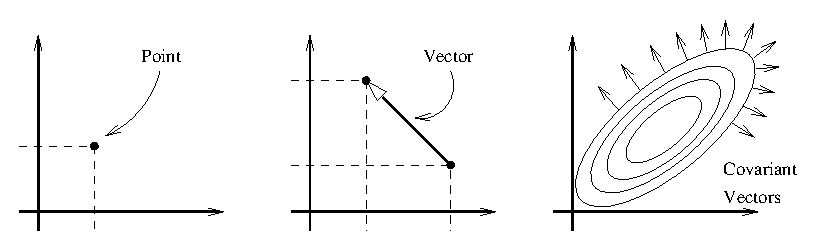
\includegraphics[width=0.9\textwidth]{GeometricalObjects.eps}
\itkcaption[Geometrical representation objects in ITK]{Geometric
representation objects in ITK.}
\label{fig:GeometricalObjects}
\end{figure}
 
ITK implements a consistent geometric representation of the space. The
characteristics of classes involved in this representation are summarized in
Table~\ref{tab:GeometricalConcepts}. In this regard, ITK takes full advantage
of the capabilities of Object Oriented programming and resists the temptation
of using simple arrays of \code{float} or \code{double} in order to represent
geometrical objects. The use of basic arrays would have blurred the important
distinction between the different geometrical concepts and would have allowed
for the innumerable conceptual and programming errors that result from using a
vector where a point is needed or vice versa.

\index{itk::Point!Concept}
\index{itk::Vector!Concept}
\index{itk::CovariantVector!Concept}

\begin{table}
\begin{center}
\begin{tabular}{ | p{0.3\textwidth} | p{ 0.6\textwidth} | }
\hline
\textbf{Class} &
\textbf{Geometrical concept} \\
\hline\hline
\doxygen{itk}{Point} & 
Position in space. In $N$-dimensional space it is represented by an array of
$N$ numbers associated with space coordinates. \\
\hline
\doxygen{itk}{Vector} & 
Relative position between two points. In $N$-dimensional space it is
represented by an array of $N$ numbers, each one associated with the distance
along a coordinate axis. Vectors do not have a position in space. A vector is
defined as the subtraction of two points.\\
\hline
\doxygen{itk}{CovariantVector} & Orthogonal direction to a $(N-1)$-dimensional
manifold in space. For example, in $3D$ it corresponds to the vector orthogonal
to a surface. This is the appropriate class for representing Gradients of
functions. Covariant vectors do not have a position in space. Covariant vector
should not be added to Points, nor to Vectors.\\
\hline
\end{tabular}
\end{center}
\itkcaption[Geometrical Elementary Objects]{Summary of objects representing
geometrical concepts in ITK.\label{tab:GeometricalConcepts}}
\end{table}


Additional uses of the \doxygen{itk}{Point}, \doxygen{itk}{Vector} and
\doxygen{itk}{CovariantVector} classes have been discussed in Chapter
\ref{sec:DataRepresentation}.  Each one of these classes behaves differently
under spatial transformations. It is therefore quite important to keep their
distinction clear. Figure
\ref{fig:GeometricalObjects} illustrates the differences between
these concepts.


\index{itk::Transform!TransformPoint()}
\index{itk::Transform!TransformVector()}
\index{itk::Transform!TransformCovariantVector()}

Transform classes provide different methods for mapping each one of
the basic space-representation objects.  Points, vectors and covariant vectors
are transformed using the methods \code{TransformPoint()},
\code{TransformVector()} and \code{TransformCovariantVector()} respectively.

One of the classes that deserve further comments is the \doxygen{itk}{Vector}. This
ITK class tend to be misinterpreted as a container of elements instead of a
geometrical object. This is a common misconception originated by the fact that
Computer Scientist and Software Engineers misuse the term ``Vector''.  The
actual word ``Vector'' is relatively young. It was coined by William Hamilton
in his book ``\emph{Elements of Quaternions}'' published in 1886
(post-mortem)\cite{Hamilton1866}.  In the same text Hamilton coined the terms:
``\emph{Scalar}'', ``\emph{Versor}'' and ``\emph{Tensor}''.  Although the
modern term of ``\emph{Tensor}'' is used in Calculus in a different sense of
what Hamilton defined in his book at the time~\cite{Dodson1997}.

A ``\emph{Vector}'' is, by definition, a mathematical object that embodies the
concept of ``direction in space''. Strictly speaking, a Vector describes the
relationship between two Points in space, and captures both their relative
distance and orientation.

Computer scientists and software engineers misused the term vector in order to
represent the concept of an ``Indexed Set''~\cite{Austern1999}.  Mechanical
Engineers and Civil Engineers, who deal with the real world of physical objects
will not commit this mistake and will keep the word ``\emph{Vector}'' attached
to a geometrical concept.  Biologists, on the other hand, will associate
``\emph{Vector}'' to a ``vehicle'' that allows them to direct something in a
particular direction, for example, a virus that allows them to insert pieces of
code into a DNA strand~\cite{Lodish2000}.

Textbooks in programming do not help to clarify those concepts and loosely use
the term ``\emph{Vector}'' for the purpose of representing an ``enumerated set
of common elements''. STL follows this trend and continue using the word
``\emph{Vector}'' for what it was not supposed to be
used~\cite{Austern1999,Alexandrescu2001}. Linear algebra separates the
``\emph{Vector}'' from its notion of geometric reality and makes it an
abstract set of numbers with arithmetic operations associated.

For those of you who are looking for the ``\emph{Vector}'' in the Software
Engineering sense, please look at the \doxygen{itk}{Array} and \doxygen{itk}{FixedArray}
classes that actually provide such functionalities. Additionally, the
\doxygen{itk}{VectorContainer} and \doxygen{itk}{MapContainer} classes may be of interest
too. These container classes are intended for algorithms that require to insert
and delete elements, and that may have large numbers of elements.

The Insight Toolkit deals with real objects that inhabit the physical space.
This is particularly true in the context of the image registration framework.
We chose to give the appropriate name to the mathematical objects that describe
geometrical relationships in N-Dimensional space. It is for this reason that we
explicitly make clear the distinction between Point, Vector and CovariantVector,
despite the fact that most people would be happy with a simple use of
\code{double[3]} for the three concepts and then will proceed to perform all
sort of conceptually flawed operations such as 

\begin{itemize}
\item Adding two Points
\item Dividing a Point by a Scalar
\item Adding a Covariant Vector to a Point
\item Adding a Covariant Vector to a Vector
\end{itemize}

In order to enforce the correct use of the Geometrical concepts in ITK we
organized these classes in a hierarchy that supports reuse of code and yet
compartmentalize the behavior of the individual classes.  The use of the
\doxygen{itk}{FixedArray} as base class of the \doxygen{itk}{Point}, the \doxygen{itk}{Vector}
and the \doxygen{itk}{CovariantVector} was a design decision based on calling things
by their correct name.

An \doxygen{itk}{FixedArray} is an enumerated collection with a fixed number of
elements. You can instantiate a fixed array of letters, or a fixed array of
images, or a fixed array of transforms, or a fixed array of geometrical shapes.
Therefore, the FixedArray only implements the functionality that is necessary to
access those enumerated elements. No assumptions can be made at this point on
any other operations required by the elements of the FixedArray, except the
fact of having a default constructor.

The \doxygen{itk}{Point} is a type that represents the spatial coordinates of a
spatial location. Based on geometrical concepts we defined the valid operations
of the Point class. In particular we made sure that no \code{operator+()} was
defined between Points, and that no \code{operator*( scalar )} nor
\code{operator/( scalar )} were defined for Points.

In other words, you could do in ITK operations such as:

\begin{itemize}
\item Vector  = Point - Point
\item Point  +=  Vector
\item Point  -=  Vector
\item Point  = BarycentricCombination( Point, Point )
\end{itemize}

and you cannot (because you \textbf{should not}) do operation such as

\begin{itemize}
\item Point = Point * Scalar    
\item Point = Point + Point    
\item Point = Point / Scalar  
\end{itemize}

The \doxygen{itk}{Vector} is, by Hamilton's definition, the subtraction between two
points. Therefore a Vector must satisfy the following basic operations:

\begin{itemize}
\item Vector = Point - Point
\item Point  = Point + Vector
\item Point  = Point - Vector
\item Vector = Vector + Vector
\item Vector = Vector - Vector
\end{itemize}

An \doxygen{itk}{Vector} object is intended to be instantiated over elements that
support mathematical operation such as addition, subtraction and multiplication
by scalars.


\subsection{Transform General Properties}
\label{sec:TransformGeneralProperties}

\index{itk::Transform!SetParameters()} Each transform class typically has
several methods for setting its parameters.  For example,
\doxygen{itk}{Euler2DTransform} provides methods for specifying the offset,
angle, and the entire rotation matrix.  However, for use in the
registration framework, the parameters are represented by a flat
Array of doubles to facilitate communication with generic
optimizers. In the case of the Euler2DTransform, the transform is also
defined by three doubles: the first representing the angle, and the last two the
offset. The flat array of parameters is defined using \code{SetParameters()}. A
description of the parameters and their ordering is documented in the 
sections that follow.
 
In the context of registration, the transform parameters define the search
space for optimizers. That is, the goal of the optimization is to find the set
of parameters defining a transform that results in the best possible value of
an image metric. The more parameters a transform has, the longer its
computational time will be when used in a registration method since the
dimension of the search space will be equal to the number of transform
parameters.

\index{itk::Transform!GetJacobian()}

Another requirement that the registration framework imposes on the transform
classes is the computation of their Jacobians. In general, metrics require
the knowledge of the Jacobian in order to compute Metric derivatives.
The Jacobian is a matrix whose element are the partial derivatives of the
output point with respect to the array of parameters that defines the
transform:\footnote{Note that the term \emph{Jacobian} is also commonly used
for the matrix representing the derivatives of output point coordinates with
respect to input point coordinates. Sometimes the term is loosely used to
refer to the determinant of such a matrix.~\cite{Dodson1997}}

\begin{equation}
J=\left[ \begin{array}{cccc}
\frac{\partial x_{1}}{\partial p_{1}} & 
\frac{\partial x_{1}}{\partial p_{2}} & 
\cdots  & \frac{\partial x_{1}}{\partial p_{m}}\\
\frac{\partial x_{2}}{\partial p_{1}} & 
\frac{\partial x_{2}}{\partial p_{2}} & 
\cdots  & \frac{\partial x_{2}}{\partial p_{m}}\\
\vdots  & \vdots  & \ddots  & \vdots \\
\frac{\partial x_{n}}{\partial p_{1}} & 
\frac{\partial x_{n}}{\partial p_{2}} & 
\cdots  & \frac{\partial x_{n}}{\partial p_{m}}
\end{array}\right]
\end{equation}

where $\{p_i\}$ are the transform parameters and $\{x_i\}$ are the coordinates
of the output point.  Within this framework, the Jacobian is represented by an
\doxygen{itk}{Array2D} of doubles and is obtained from the transform by method
\code{GetJacobian()}. The Jacobian can be interpreted as a matrix that
indicates for a point in the input space how much its mapping on the output
space will change as a response to a small variation in one of the transform
parameters. Note that the values of the Jacobian matrix depend on the point in
the input space. So actually the Jacobian can be noted as $J(\bf{X})$, where
${\bf{X}}=\{x_i\}$. The use of transform Jacobians enables the efficient
computation of metric derivatives.  When Jacobians are not available, metrics
derivatives have to be computed using finite difference at a price of $2M$
evaluations of the metric value, where $M$ is the number of transform
parameters.

The following sections describe the main characteristics of the transform
classes available in ITK.

\subsection{Identity Transform}
\label{sec:IdentityTransform}
\index{itk::IdentityTransform}

\begin{table}
\begin{center}
\begin{tabular}{\tableconfiguration}
\hline
\textbf{Behavior} &
\textbf{Number of Parameters} &
\textbf{Parameter Ordering} &
\textbf{Restrictions} \\
\hline\hline
Maps every point to itself, every vector to itself and every covariant vector to itself.  & 
0 &
NA  &  
Only defined when the input and output space has the same number of dimensions. \\
\hline
\end{tabular}
\end{center}
\itkcaption[Identity Transform Characteristics]{Characteristics of the identity transform.
\label{tab:IdentityTransformCharacteristics}}
\end{table}

The identity transform \doxygen{itk}{IdentityTransform} is mainly used for debugging
purposes. It is provided to methods that require a transform and in cases where
we want to have the certainty that the transform will have no effect whatsoever
in the outcome of the process. It is just a \code{NULL} operation. The main
characteristics of the identity transform are summarized in
Table~\ref{tab:IdentityTransformCharacteristics}


\subsection{Translation Transform}
\label{sec:TranslationTransform}
\index{itk::TranslationTransform}

\begin{table}
\begin{center}
\begin{tabular}{\tableconfiguration}
\hline
\textbf{Behavior} &
\textbf{Number of Parameters} &
\textbf{Parameter Ordering} &
\textbf{Restrictions} \\
\hline\hline
Represents a simple translation of points in the input space
and has no effect on vectors or covariant vectors. &
Same as the input space dimension. &
The $i$-th parameter represents the translation in the $i$-th dimension. &
Only defined when the input and output space has the same number of dimensions. \\
\hline
\end{tabular}
\end{center}
\itkcaption[Translation Transform Characteristics]{Characteristics of the TranslationTransform class.
\label{tab:TranslationTransformCharacteristics}}
\end{table}

The \doxygen{itk}{TranslationTransform} is probably the simplest yet one of the most
useful transformations.  It maps all Points by adding a Vector to them.  Vector
and covariant vectors remain unchanged under this transformation since they are
not associated with a particular position in space. Translation is the best
transform to use when starting a registration method. Before attempting to
solve for rotations or scaling it is important to overlap the anatomical
objects in both images as much as possible. This is done by resolving the
translational misalignment between the images. Translations also have the
advantage of being fast to compute and having parameters that are easy to
interpret. The main characteristics of the translation transform are presented
in Table~\ref{tab:TranslationTransformCharacteristics}.

\subsection{Scale Transform}
\label{sec:ScaleTransform}
\index{itk::ScaleTransform}

\begin{table}
\begin{center}
\begin{tabular}{\tableconfiguration}
\hline
\textbf{Behavior} &
\textbf{Number of Parameters} &
\textbf{Parameter Ordering} &
\textbf{Restrictions} \\
\hline\hline
Points are transformed by multiplying each one of their coordinates by the
corresponding scale factor for the dimension.  Vectors are transformed as
points.  Covariant vectors are transformed by \emph{dividing} their components
by the scale factor in the corresponding dimension.  &
Same as the input space dimension. &
The $i$-th parameter represents the scaling in the $i$-th dimension. &
Only defined when the input and output space has the same number of dimensions. \\
\hline
\end{tabular}
\end{center}
\itkcaption[Scale Transform Characteristics]{Characteristics of the ScaleTransform class.
\label{tab:ScaleTransformCharacteristics}}
\end{table}

The \doxygen{itk}{ScaleTransform} represents a simple scaling of the
vector space.  Different scaling factors can be applied along each
dimension. Points are transformed by multiplying each one of their
coordinates by the corresponding scale factor for the dimension.  Vectors are
transformed in the same way as points.  Covariant vectors, on the other hand,
are transformed differently since anisotropic scaling does not preserve
angles. Covariant vectors are transformed by \emph{dividing} their components
by the scale factor of the corresponding dimension. In this way, if a
covariant vector was orthogonal to a vector, this orthogonality will be
preserved after the transformation. The following equations summarize the
effect of the transform on the basic geometric objects.

\begin{equation}
\begin{array}{lccccccc}
\mbox{Point }          & \bf{P'} &  =  & T(\bf{P})  & : & \bf{P'}_i &  = & \bf{P}_i \cdot S_i \\
\mbox{Vector}          & \bf{V'} &  =  & T(\bf{V})  & : & \bf{V'}_i &  = & \bf{V}_i \cdot S_i \\
\mbox{CovariantVector} & \bf{C'} &  =  & T(\bf{C})  & : & \bf{C'}_i &  = & \bf{C}_i /     S_i \\
\end{array}
\end{equation}

where $\bf{P}_i$, $\bf{V}_i$ and $\bf{C}_i$ are the point, vector and covariant
vector $i$-th components while $\bf{S}_i$ is the scaling factor along dimension
$i-th$.  The following equation illustrates the effect of the scaling transform
on a $3D$ point.

\begin{equation}
\left[ 
\begin{array}{c}
x' \\
y' \\
z' \\
\end{array}
\right]
=
\left[ 
\begin{array}{ccc}
S_1 &  0  &  0  \\
 0  & S_2 &  0  \\
 0  &  0  & S_3 \\
\end{array}
\right]
\cdot
\left[ 
\begin{array}{c}
x  \\
y  \\
z  \\
\end{array}
\right]
\end{equation}

Scaling appears to be a simple transformation but there are actually a
number of issues to keep in mind when using different scale factors along
every dimension. There are subtle effects---for example, when computing image
derivatives. Since derivatives are represented by covariant vectors, their
values are not intuitively modified by scaling transforms.

One of the difficulties with managing scaling transforms in a registration
process is that typical optimizers manage the parameter space as a vector
space where addition is the basic operation. Scaling is better treated in the
frame of a logarithmic space where additions result in regular multiplicative
increments of the scale. Gradient descent optimizers have trouble updating
step length, since the effect of an additive increment on a scale factor
diminishes as the factor grows. In other words, a scale factor variation of
$(1.0+ \epsilon)$ is quite different from a scale variation of
$(5.0+\epsilon)$.

Registrations involving scale transforms require careful monitoring of the
optimizer parameters in order to keep it progressing at a stable pace. Note
that some of the transforms discussed in following sections, for example, the
AffineTransform, have hidden scaling parameters and are therefore
subject to the same vulnerabilities of the ScaleTransform.

In cases involving misalignments with simultaneous translation, rotation and
scaling components it may be desirable to solve for these components
independently. The main characteristics of the scale transform are presented in
Table~\ref{tab:ScaleTransformCharacteristics}.


\subsection{Scale Logarithmic Transform}
\label{sec:ScaleLogarithmicTransform}
\index{itk::Scale\-Logarithmic\-Transform}

\begin{table}
\begin{center}
\begin{tabular}{\tableconfiguration}
\hline
\textbf{Behavior} &
\textbf{Number of Parameters} &
\textbf{Parameter Ordering} &
\textbf{Restrictions} \\
\hline\hline
Points are transformed by multiplying each one of their coordinates by the
corresponding scale factor for the dimension.  Vectors are transformed as
points.  Covariant vectors are transformed by \emph{dividing} their components
by the scale factor in the corresponding dimension. 
&
Same as the input space dimension. &
The $i$-th parameter represents the scaling in the $i$-th dimension. &
Only defined when the input and output space has the same number of dimensions.
The difference between this transform and the ScaleTransform is that here the
scaling factors are passed as logarithms, in this way their behavior is closer
to the one of a Vector space.  \\
\hline
\end{tabular}
\end{center}
\itkcaption[Scale Logarithmic Transform Characteristics]{Characteristics of the ScaleLogarithmicTransform class.
\label{tab:ScaleLogarithmicTransformCharacteristics}}
\end{table}

The \doxygen{itk}{ScaleLogarithmicTransform} is a simple variation of the
\doxygen{itk}{ScaleTransform}. It is intended to improve the behavior of the scaling
parameters when they are modified by optimizers. The difference between this
transform and the ScaleTransform is that the parameter factors are passed here
as logarithms. In this way, multiplicative variations in the scale become
additive variations in the logarithm of the scaling factors.




\subsection{Euler2DTransform}
\label{sec:Euler2DTransform}
\index{itk::Euler2DTransform}

\begin{table}
\begin{center}
\begin{tabular}{\tableconfiguration}
\hline
\textbf{Behavior} &
\textbf{Number of Parameters} &
\textbf{Parameter Ordering} &
\textbf{Restrictions} \\
\hline\hline
Represents a $2D$ rotation and a $2D$ translation. Note that the translation
component has no effect on the transformation of vectors and covariant vectors. &
3 &
The first parameter is the angle in radians and the last two parameters
are the translation in each dimension. &
Only defined for two-dimensional input and output spaces. \\
\hline
\end{tabular}
\end{center}
\itkcaption[Euler2D Transform Characteristics]{Characteristics of the Euler2DTransform class.
\label{tab:Euler2DTransformCharacteristics}}
\end{table}

\doxygen{itk}{Euler2DTransform} implements a rigid transformation in $2D$. It is 
composed of a plane rotation and a two-dimensional translation. The rotation
is applied first, followed by the translation. The following equation
illustrates the effect of this transform on a $2D$ point,


\begin{equation}
\left[ 
\begin{array}{c}
x' \\
y' \\
\end{array}
\right]
=
\left[ 
\begin{array}{cc}
\cos{\theta} & -\sin{\theta} \\
\sin{\theta} &  \cos{\theta} \\
\end{array}
\right]
\cdot
\left[ 
\begin{array}{c}
x  \\
y  \\
\end{array}
\right]
+ 
\left[ 
\begin{array}{c}
T_x  \\
T_y  \\
\end{array}
\right]
\end{equation}

where $\theta$ is the rotation angle and $(T_x,T_y)$ are the components of the
translation.

A challenging aspect of this transformation is the fact that translations and
rotations do not form a vector space and cannot be managed as linear
independent parameters. Typical optimizers make the loose assumption that
parameters exist in a vector space and rely on the step length to be small
enough for this assumption to hold approximately.

In addition to the non-linearity of the parameter space, the most common
difficulty found when using this transform is the difference in units used
for rotations and translations. Rotations are measured in radians; hence,
their values are in the range $[-\pi,\pi]$. Translations are measured in
millimeters and their actual values vary depending on the image modality
being considered. In practice, translations have values on the order of $10$
to $100$. This scale difference between the rotation and translation
parameters is undesirable for gradient descent optimizers because they
deviate from the trajectories of descent and make optimization slower and more
unstable. In order to compensate for these differences, ITK optimizers accept
an array of scale values that are used to normalize the parameter space.

Registrations involving angles and translations should take advantage of the
scale normalization functionality in order to obtain the best performance out
of the optimizers. The main characteristics of the Euler2DTransform class
are presented in Table~\ref{tab:Euler2DTransformCharacteristics}.


\subsection{CenteredRigid2DTransform}
\label{sec:CenteredRigid2DTransform}
\index{itk::Centered\-Rigid2D\-Transform}

\begin{table}
\begin{center}
\begin{tabular}{\tableconfiguration}
\hline
\textbf{Behavior} &
\textbf{Number of Parameters} &
\textbf{Parameter Ordering} &
\textbf{Restrictions} \\
\hline\hline
Represents a $2D$ rotation around a user-provided center followed by a $2D$ translation.&
5 &
The first parameter is the angle in radians. Second and third are the center of
rotation coordinates and the last two parameters are the translation in each
dimension. & 
Only defined for two-dimensional input and output spaces. \\
\hline
\end{tabular}
\end{center}
\itkcaption[CenteredRigid2D Transform Characteristics]{Characteristics of the CenteredRigid2DTransform class.
\label{tab:CenteredRigid2DTransformCharacteristics}}
\end{table}

\doxygen{itk}{CenteredRigid2DTransform} implements a rigid transformation in $2D$.
The main difference between this transform and the \doxygen{itk}{Euler2DTransform}
is that here we can specify an arbitrary center of rotation, while the
Euler2DTransform always uses the origin of the coordinate system as the center
of rotation. This distinction is quite important in image registration since
ITK images usually have their origin in the corner of the image rather than the
middle.  Rotational mis-registrations usually exist, however, as rotations
around the center of the image, or at least as rotations around a point in the
middle of the anatomical structure captured by the image. Using gradient
descent optimizers, it is almost impossible to solve non-origin rotations using
a transform with origin rotations since the deep basin of the real solution is
usually located across a high ridge in the topography of the cost function.

In practice, the user must supply the center of rotation in the input space,
the angle of rotation and a translation to be applied after the rotation. With
these parameters, the transform initializes a rotation matrix and a translation
vector that together perform the equivalent of translating the center of
rotation to the origin of coordinates, rotating by the specified angle,
translating back to the center of rotation and finally translating by the
user-specified vector.

As with the Euler2DTransform, this transform suffers from the difference in
units used for rotations and translations. Rotations are measured in radians;
hence, their values are in the range $[-\pi,\pi]$. The center of rotation and
the translations are measured in millimeters, and their actual values vary
depending on the image modality being considered.  Registrations involving
angles and translations should take advantage of the scale normalization
functionality of the optimizers in order to get the best performance out of
them.

The following equation illustrates the effect of the transform on an input
point $(x,y)$ that maps to the output point $(x',y')$,

\begin{equation}
\left[ 
\begin{array}{c}
x' \\
y' \\
\end{array}
\right]
=
\left[ 
\begin{array}{cc}
\cos{\theta} & -\sin{\theta} \\
\sin{\theta} &  \cos{\theta} \\
\end{array}
\right]
\cdot
\left[ 
\begin{array}{c}
x - C_x \\
y - C_y \\
\end{array}
\right]
+ 
\left[ 
\begin{array}{c}
T_x + C_x \\
T_y + C_y \\
\end{array}
\right]
\end{equation}

where $\theta$ is the rotation angle, $(C_x,C_y)$ are the coordinates of the
rotation center and $(T_x,T_y)$ are the components of the translation. Note
that the center coordinates are subtracted before the rotation and added back
after the rotation. The main features of the CenteredRigid2DTransform are 
presented in Table~\ref{tab:CenteredRigid2DTransformCharacteristics}.


\subsection{Similarity2DTransform}
\label{sec:Similarity2DTransform}
\index{itk::Similarity2DTransform}

\begin{table}
\begin{center}
\begin{tabular}{\tableconfiguration}
\hline
\textbf{Behavior} &
\textbf{Number of Parameters} &
\textbf{Parameter Ordering} &
\textbf{Restrictions} \\
\hline\hline
Represents a $2D$ rotation, homogeneous scaling and a $2D$ translation. Note that
the translation component has no effect on the transformation of vectors and
covariant vectors. & 
4 &
The first parameter is the scaling factor for all dimensions, the second is the
angle in radians, and the last two parameters are the translations in $(x,y)$
respectively. & 
Only defined for two-dimensional input and output spaces. \\
\hline
\end{tabular}
\end{center}
\itkcaption[Similarity2D Transform Characteristics]{Characteristics of the Similarity2DTransform class.
\label{tab:Similarity2DTransformCharacteristics}}
\end{table}

The \doxygen{itk}{Similarity2DTransform} can be seen as a rigid transform combined
with an isotropic scaling factor. This transform preserves angles between
lines. In its $2D$ implementation, the four parameters of this transformation
combine the characteristics of the \doxygen{itk}{ScaleTransform} and
\doxygen{itk}{Euler2DTransform}. In particular, those relating to the non-linearity
of the parameter space and the non-uniformity of the measurement units.
Gradient descent optimizers should be used with caution on such parameter
spaces since the notions of gradient direction and step length are ill-defined.

The following equation illustrates the effect of the transform on an input
point $(x,y)$ that maps to the output point $(x',y')$,

\begin{equation}
\left[ 
\begin{array}{c}
x' \\
y' \\
\end{array}
\right]
=
\left[ 
\begin{array}{cc}
\lambda &    0     \\
   0    &  \lambda \\
\end{array}
\right]
\cdot
\left[ 
\begin{array}{cc}
\cos{\theta} & -\sin{\theta} \\
\sin{\theta} &  \cos{\theta} \\
\end{array}
\right]
\cdot
\left[ 
\begin{array}{c}
x - C_x \\
y - C_y \\
\end{array}
\right]
+ 
\left[ 
\begin{array}{c}
T_x + C_x \\
T_y + C_y \\
\end{array}
\right]
\end{equation}

where $\lambda$ is the scale factor, $\theta$ is the rotation angle,
$(C_x,C_y)$ are the coordinates of the rotation center and $(T_x,T_y)$ are the
components of the translation. Note that the center coordinates are subtracted
before the rotation and scaling, and they are added back afterwards.  The main
features of the Similarity2DTransform are presented in
Table~\ref{tab:Similarity2DTransformCharacteristics}.


A possible approach for controlling optimization in the parameter space of
this transform is to dynamically modify the array of scales passed to the
optimizer. The effect produced by the parameter scaling can be used to steer
the walk in the parameter space (by giving preference to some of the
parameters over others). For example, perform some iterations updating only
the rotation angle, then balance the array of scale factors in the optimizer
and perform another set of iterations updating only the translations.


\subsection{QuaternionRigidTransform}
\label{sec:QuaternionRigidTransform}
\index{itk::Quaternion\-Rigid\-Transform}

\begin{table}
\begin{center}
\begin{tabular}{| p{4cm} | p{1.8cm} | p{2.5cm} | p{3cm} |}
\hline
\textbf{Behavior} &
\textbf{Number of Parameters} &
\textbf{Parameter Ordering} &
\textbf{Restrictions} \\
\hline\hline
Represents a $3D$ rotation and a $3D$ translation. The rotation is specified as a
quaternion, defined by a set of four numbers $\bf{q}$.  The relationship
between quaternion and rotation about vector $\bf{n}$ by angle $\theta$ is as
follows: \[ \bf{q} = (\bf{n}\sin(\theta/2), \cos(\theta/2))\] Note that if the
quaternion is not of unit length, scaling will also result. &
7 &
The first four parameters defines the quaternion and the last three parameters
the translation in each dimension. &
Only defined for three-dimensional input and output spaces. \\
\hline
\end{tabular}
\end{center}
\itkcaption[QuaternionRigid Transform Characteristics]{Characteristics of the QuaternionRigidTransform class.
\label{tab:QuaternionRigidTransformCharacteristics}}
\end{table}

The \doxygen{itk}{QuaternionRigidTransform} class implements a rigid
transformation in $3D$ space. The rotational part of the transform is
represented using a quaternion while the translation is represented with a
vector. Quaternions components do not form a vector space and hence raise the
same concerns as the \doxygen{itk}{Similarity2DTransform} when used with gradient
descent optimizers.

The \doxygen{itk}{QuaternionRigidTransformGradientDescentOptimizer} was introduced into the toolkit to address these concerns.  This specialized optimizer implements a variation of a
gradient descent algorithm adapted for a quaternion space.  This class
insures that after advancing in any direction on the parameter space, the
resulting set of transform parameters is mapped back into the permissible
set of parameters. In practice, this comes down to normalizing the newly-computed quaternion to make sure that the transformation remains rigid and no
scaling is applied.  The main characteristics of the
QuaternionRigidTransform are presented in
Table~\ref{tab:QuaternionRigidTransformCharacteristics}.

The Quaternion rigid transform also accepts a user-defined center of rotation.
In this way, the transform can easily be used for registering images where the
rotation is mostly relative to the center of the image instead one of the
corners. The coordinates of this rotation center are not subject to
optimization. They only participate in the computation of the mappings for
Points and in the computation of the Jacobian. The transformations for Vectors
and CovariantVector are not affected by the selection of the rotation center.



\subsection{VersorTransform}
\label{sec:VersorTransform}
\index{itk::VersorTransform}
\index{itk::VersorTransformOptimizer}
\index{itk::Versor!Definition}

\begin{table}
\begin{center}
\begin{tabular}{\tableconfiguration}
\hline
\textbf{Behavior} &
\textbf{Number of Parameters} &
\textbf{Parameter Ordering} &
\textbf{Restrictions} \\
\hline\hline
Represents a $3D$ rotation. The rotation is specified by a versor or unit
quaternion. The rotation is performed around a user-specified center of
rotation.&
3 &
The three parameters define the versor.&
Only defined for three-dimensional input and output spaces. \\
\hline
\end{tabular}
\end{center}
\itkcaption[Versor Transform Characteristics]{Characteristics of the Versor Transform
\label{tab:VersorTransformCharacteristics}}
\end{table}


By definition, a \emph{Versor} is the rotational part of a Quaternion. It can
also be defined as a \emph{unit-quaternion} \cite{Hamilton1866,Joly1905}.
Versors only have three independent components, since they are restricted to
reside in the space of unit-quaternions. The implementation of versors in the
toolkit uses a set of three numbers.  These three numbers correspond to the
first three components of a quaternion.  The fourth component of the quaternion
is computed internally such that the quaternion is of unit length. The main
characteristics of the \doxygen{itk}{VersorTransform} are presented in
Table~\ref{tab:VersorTransformCharacteristics}.

This transform exclusively represents rotations in $3D$. It is intended to
rapidly solve the rotational component of a more general misalignment.  The
efficiency of this transform comes from using a parameter space of reduced
dimensionality. Versors are the best possible representation for rotations in
$3D$ space. Sequences of versors allow the creation of smooth rotational
trajectories; for this reason, they behave stably under optimization methods.

The space formed by versor parameters is not a vector space. Standard gradient
descent algorithms are not appropriate for exploring this parameter space. An
optimizer specialized for the versor space is available in the toolkit under
the name of \doxygen{itk}{VersorTransformOptimizer}. This optimizer implements
versor derivatives as originally defined by Hamilton \cite{Hamilton1866}.

The center of rotation can be specified by the user with the
\code{SetCenter()} method. The center is not part of the parameters to be
optimized, therefore it remains the same during an optimization process. Its
value is used during the computations for transforming Points and when
computing the Jacobian.

\subsection{VersorRigid3DTransform}
\label{sec:VersorRigid3DTransform}
\index{itk::VersorRigid3DTransform}

\begin{table}
\begin{center}
\begin{tabular}{\tableconfiguration}
\hline
\textbf{Behavior} &
\textbf{Number of Parameters} &
\textbf{Parameter Ordering} &
\textbf{Restrictions} \\
\hline\hline
Represents a $3D$ rotation and a $3D$ translation. The rotation is specified by
a versor or unit quaternion, while the translation is represented by a vector.
Users can specify the coordinates of the center of rotation. &
6 &
The first three parameters define the versor and the last three parameters the
translation in each dimension. &
Only defined for three-dimensional input and output spaces. \\
\hline
\end{tabular}
\end{center}
\itkcaption[Versor Rigid3D Transform Characteristics]{Characteristics of the VersorRigid3DTransform class.
\label{tab:VersorRigid3DTransformCharacteristics}}
\end{table}

The \doxygen{itk}{VersorRigid3DTransform} implements a rigid transformation in $3D$
space. It is a variant of the \doxygen{itk}{QuaternionRigidTransform} and the
\doxygen{itk}{VersorTransform}. It can be seen as a \doxygen{itk}{VersorTransform} plus a
translation defined by a vector. The advantage of this class with respect to
the QuaternionRigidTransform is that it exposes only six parameters, three for
the versor components and three for the translational components. This reduces
the search space for the optimizer to six dimensions instead of the seven
dimensional used by the QuaternionRigidTransform.  This transform also allows
the users to set a specific center of rotation. The center coordinates are not
modified during the optimization performed in a registration process.  The main
features of this transform are summarized in
Table~\ref{tab:VersorRigid3DTransformCharacteristics}.  This transform is
probably the best option to use when dealing with rigid transformations in
$3D$. 

Given that the space of Versors is not a Vector space, typical gradient descent
optimizers are not well suited for exploring the parametric space of this
transform. The \doxygen{itk}{VersorRigid3DTranformOptimizer} has been
introduced in the ITK toolkit with the purpose of providing an optimizer that
is aware of the Versor space properties on the rotational part of this
transform, as well as the Vector space properties on the translational part of
the transform.


\subsection{Euler3DTransform}
\label{sec:Euler3DTransform}
\index{itk::Euler3DTransform}

\begin{table}
\begin{center}
\begin{tabular}{\tableconfiguration}
\hline
\textbf{Behavior} &
\textbf{Number of Parameters} &
\textbf{Parameter Ordering} &
\textbf{Restrictions} \\
\hline\hline
Represents a rigid rotation in $3D$ space. That is, a rotation followed by a
$3D$ translation. The rotation is specified by three angles representing
rotations to be applied around the X, Y and Z axis one after another.  The
translation part is represented by a Vector. Users can also specify the
coordinates of the center of rotation. &
6 &
The first three parameters are the rotation angles around X, Y and Z axis, and
the last three parameters are the translations along each dimension. &
Only defined for three-dimensional input and output spaces. \\
\hline
\end{tabular}
\end{center}
\itkcaption[Euler3D Transform Characteristics]{Characteristics of the Euler3DTransform class.
\label{tab:Euler3DTransformCharacteristics}}
\end{table}

The \doxygen{itk}{Euler3DTransform} implements a rigid transformation in $3D$ space.
It can be seen as a rotation followed by a translation. This class exposes six
parameters, three for the Euler angles that represent the rotation and three
for the translational components. This transform also allows the users to set a
specific center of rotation. The center coordinates are not modified during the
optimization performed in a registration process. The main features of this
transform are summarized in Table~\ref{tab:Euler3DTransformCharacteristics}.  

The fact that the three rotational parameters are non-linear and do not behave
like Vector spaces must be taken into account when selecting an optimizer to
work with this transform and when fine tuning the parameters of such
optimizer. It is strongly recommended to use this transform by introducing very
small variations on the rotational components. A small rotation will be in the
range of 1 degree, which in radians is approximately $0.0.1745$.

You should not expect this transform to be able to compensate for large
rotations just by being driven with the optimizer. In practice you must provide
a reasonable initialization of the transform angles and only need to correct
for residual rotations in the order of $10$ or $20$ degrees.


\subsection{Similarity3DTransform}
\label{sec:Similarity3DTransform}
\index{itk::Similarity3DTransform}

\begin{table}
\begin{center}
\begin{tabular}{\tableconfiguration}
\hline
\textbf{Behavior} &
\textbf{Number of Parameters} &
\textbf{Parameter Ordering} &
\textbf{Restrictions} \\
\hline\hline
Represents a $3D$ rotation, a $3D$ translation and homogeneous scaling. The
scaling factor is specified by a scalar, the rotation is specified by a versor,
and the translation is represented by a vector.  Users can also specify the
coordinates of the center of rotation, that is the same center used for
scaling. &
7 &
The first parameter is the scaling factor, the next three parameters define the
versor and the last three parameters the translation in each dimension. &
Only defined for three-dimensional input and output spaces. \\
\hline
\end{tabular}
\end{center}
\itkcaption[Similarity3D Transform Characteristics]{Characteristics of the Similarity3DTransform class.
\label{tab:Similarity3DTransformCharacteristics}}
\end{table}

The \doxygen{itk}{Similarity3DTransform} implements a similarity transformation in
$3D$ space. It can be seen as an homogeneous scaling followed by a
\doxygen{itk}{VersorRigid3DTransform}. This class exposes seven parameters, one for
the scaling factor, three for the versor components and three for the
translational components. This transform also allows the users to set a
specific center of rotation. The center coordinates are not modified during the
optimization performed in a registration process.  Both the rotation and
scaling operations are performed with respect to the center of rotation. The
main features of this transform are summarized in
Table~\ref{tab:Similarity3DTransformCharacteristics}.  

The fact that the scaling and rotational spaces are non-linear and do not
behave like Vector spaces must be taken into account when selecting an
optimizer to work with this transform and when fine tuning the parameters of
such optimizer.


\subsection{Rigid3DPerspectiveTransform}
\label{sec:Rigid3DPerspectiveTransform}
\index{itk::Rigid3D\-Perspective\-Transform}

\begin{table}
\begin{center}
\begin{tabular}{\tableconfiguration}
\hline
\textbf{Behavior} &
\textbf{Number of Parameters} &
\textbf{Parameter Ordering} &
\textbf{Restrictions} \\
\hline\hline 
Represents a rigid $3D$ transformation followed by a perspective projection.
The rotation is specified by a Versor, while the translation is represented by
a Vector.  Users can specify the coordinates of the center of rotation. They
must specifically a focal distance to be used for the perspective projection. The
rotation center and the focal distance parameters are not modified during the
optimization process. &
6 &
The first three parameters define the Versor and the last three parameters the
Translation in each dimension. &
Only defined for three-dimensional input and two-dimensional output spaces.
This is one of the few transforms where the input space has a different
dimension from the output space.\\
\hline
\end{tabular}
\end{center}
\itkcaption[Rigid3DPerspective Transform Characteristics]{Characteristics of
the Rigid3DPerspectiveTransform class.
\label{tab:Rigid3DPerspectiveTransformCharacteristics}}
\end{table}

The \doxygen{itk}{Rigid3DPerspectiveTransform} implements a rigid transformation in
$3D$ space followed by a perspective projection. This transform is intended to
be used in $3D/2D$ registration problems where a 3D object is projected onto a
2D plane. This is the case of Fluoroscopic images used for image guided
intervention, and it is also the case for classical radiography.  Users must
provide a value for the focal distance to be used during the computation of the
perspective transform. This transform also allows users to set a specific
center of rotation. The center coordinates are not modified during the
optimization performed in a registration process.  The main features of this
transform are summarized in
Table~\ref{tab:Rigid3DPerspectiveTransformCharacteristics}.  This transform is also
used when creating Digitally Reconstructed Radiographs (DRRs).

The strategies for optimizing the parameters of this transform are the same
ones used for optimizing the VersorRigid3DTransform. In particular, you can use
the same Versor\-Rigid3D\-Tranform\-Optimizer in order to optimize the
parameters of this class.


\subsection{AffineTransform}
\label{sec:AffineTransform}
\index{itk::AffineTransform}

\begin{table}
\begin{center}
\begin{tabular}{\tableconfiguration}
\hline
\textbf{Behavior} &
\textbf{Number of Parameters} &
\textbf{Parameter Ordering} &
\textbf{Restrictions} \\
\hline\hline
Represents an affine transform composed of rotation, scaling, shearing and
translation. The transform is specified by a $N \times N$ matrix and a $N
\times 1$ vector where $N$ is the space dimension. &
$(N+1) \times N$ &
The first $N \times N$ parameters define the matrix in column-major order
(where the column index varies the fastest).  The last $N$ parameters define
the translations for each dimension. &
Only defined when the input and output space have the same dimension. \\
\hline
\end{tabular}
\end{center}
\itkcaption[Affine Transform Characteristics]{Characteristics of the AffineTransform class.
\label{tab:AffineTransformCharacteristics}}
\end{table}

The \doxygen{itk}{AffineTransform} is one of the most popular transformations used
for image registration. Its main advantage comes from the fact that it is 
represented as a linear transformation. The main features of this
transform are presented in Table~\ref{tab:AffineTransformCharacteristics}.

The set of AffineTransform coefficients can actually be represented in a vector
space of dimension $(N+1) \times N$. This makes it possible for optimizers to
be used appropriately on this search space. However, the high dimensionality of
the search space also implies a high computational complexity of cost-function
derivatives. The best compromise in the reduction of this computational time is
to use the transform's Jacobian in combination with the image gradient for
computing the cost-function derivatives.

The coefficients of the $N \times N$ matrix can represent rotations,
anisotropic scaling and shearing. These coefficients are usually of a very
different dynamic range compared to the translation
coefficients. Coefficients in the matrix tend to be in the range $[-1:1]$, but
are not restricted to this interval.  Translation coefficients, on the other
hand, can be on the order of $10$ to $100$, and are basically related to the
image size and pixel spacing.

This difference in scale makes it necessary to take advantage of the
functionality offered by the optimizers for rescaling the parameter space. This
is particularly relevant for optimizers based on gradient descent approaches.
This transform lets the user set an arbitrary center of rotation. The
coordinates of the rotation center do not make part of the parameters array
passed to the optimizer. Equation~\ref{eqn:AffineTransform} illustrates the
effect of applying the AffineTransform in a point in $3D$ space.

\begin{equation}
\label{eqn:AffineTransform}
\left[ 
\begin{array}{c}
x' \\
y' \\
z' \\
\end{array}
\right]
=
\left[ 
\begin{array}{ccc}
M_{00} & M_{01} & M_{02} \\
M_{10} & M_{11} & M_{12} \\
M_{20} & M_{21} & M_{22} \\
\end{array}
\right]
\cdot
\left[ 
\begin{array}{c}
x - C_x \\
y - C_y \\
z - C_z \\
\end{array}
\right]
+ 
\left[ 
\begin{array}{c}
T_x + C_x \\
T_y + C_y \\
T_z + C_z \\
\end{array}
\right]
\end{equation}


A registration based on the affine transform may be more effective when
applied after simpler transformations have been used to remove the major
components of misalignment. Otherwise it will incur an overwhelming
computational cost. For example, using an affine transform, the first set of
optimization iterations would typically focus on removing large
translations. This task could instead be accomplished by a translation
transform in a parameter space of size $N$ instead of the $(N+1) \times N$
associated with the affine transform.

Tracking the evolution of a registration process that uses
AffineTransforms can be challenging, since it is difficult to
represent the coefficients in a meaningful way.  A simple printout of the
transform coefficients generally does not offer a clear picture of the current
behavior and trend of the optimization.  A better implementation uses
the affine transform to deform wire-frame cube which is shown in a $3D$
visualization display.



\subsection{BSplineDeformableTransform}
\label{sec:BSplineDeformableTransform}
\index{itk::BSpline\-Deformable\-Transform}

\begin{table}
\begin{center}
\begin{tabular}{\tableconfiguration}
\hline
\textbf{Behavior} &
\textbf{Number of Parameters} &
\textbf{Parameter Ordering} &
\textbf{Restrictions} \\
\hline\hline
Represents a free from deformation by providing a deformation field from the
interpolation of deformations in a coarse grid. 
&
$M \times N$ &
Where $M$ is the number of nodes in the BSpline grid and $N$ is the dimension of the space. &
Only defined when the input and output space have the same dimension. This
transform has the advantage of allowing to compute deformable registration. It
also has the disadvantage of having a very high dimensional parametric space,
and therefore requiring long computation times.\\
\hline
\end{tabular}
\end{center}
\itkcaption[BSpline Deformable Transform Characteristics]{Characteristics of the BSplineDeformableTransform class.
\label{tab:BSplineDeformableTransformCharacteristics}}
\end{table}

The \doxygen{itk}{BSplineDeformableTransform} is designed to be used for solving
deformable registration problems. This transform is equivalent to generation a
deformation field where a deformation vector is assigned to every point in
space.  The deformation vectors are computed using BSpline interpolation from
the deformation values of points located in a coarse grid, that is usually
referred to as the BSpline grid.

The BSplineDeformableTransform is not flexible enough for accounting for large
rotations or shearing, or scaling differences. In order to compensate for this
limitation, it provides the functionality of being composed with an arbitrary
transform. This transform is known as the \emph{Bulk} transform and it is
applied to points before they are mapped with the displacement field.

This transform do not provide functionalities for mapping Vectors nor
CovariantVectors, only Points can be mapped. The reason is that the variations
of a vector under a deformable transform actually depend on the location of the
vector in space. In other words, Vector only make sense as the relative
position between two points.

The BSplineDeformableTransform has a very large number of parameters and
therefore is well suited for the \doxygen{itk}{LBFGSOptimizer} and
\doxygen{itk}{LBFGSBOptimizer}. The use of this transform for was proposed in the
following papers~\cite{Rueckert1999,Mattes2001,Mattes2003}.




\subsection{KernelTransforms}
\label{sec:KernelTransforms}
\index{itk::Kernel\-Transforms}
\index{itk::Elastic\-Body\-Spline\-Kernel\-Transform}
\index{itk::Elastic\-Body\-Reciprocal\-Spline\-Kernel\-Transform}
\index{itk::Thin\-Plate\-Spline\-Kernel\-Transform}
\index{itk::Thin\-Plate\-R2\-LogR\-Spline\-Kernel\-Transform}
\index{itk::Volume\-Spline\-Kernel\-Transform}

Kernel Transforms are a set of Transforms that are also suitable for performing
deformable registration. These transforms compute on the fly the displacements
corresponding to a deformation field. The displacement values corresponding to
every point in space are computed by interpolation from the vectors defined by
a set of \emph{Source Landmarks} and a set of \emph{Target Landmarks}.

Several variations of these transforms are available in the toolkit. They
differ on the type of interpolation kernel that is used when computing the
deformation in a particular point of space. Note that these transforms are
computationally expensive and that their numerical complexity is proportional
to the number of landmarks and the space dimension.

The following is the list of Transforms based on the KernelTransform.

\begin{itemize}
\item \doxygen{itk}{ElasticBodySplineKernelTransform}
\item \doxygen{itk}{ElasticBodyReciprocalSplineKernelTransform}
\item \doxygen{itk}{ThinPlateSplineKernelTransform}
\item \doxygen{itk}{ThinPlateR2LogRSplineKernelTransform}
\item \doxygen{itk}{VolumeSplineKernelTransform}
\end{itemize}

Details about the mathematical background of these transform can be found in
the paper by Davis \emph{et. al}~\cite{Davis1997} and the papers by Rohr
\emph{et. al}~\cite{Rohr1999,Rohr2001}.



%% \fi



%% % the clearpage command helps to avoid orphans in the title of the next
%% % section.
%% \clearpage

%% \section{Interpolators}
%% \label{sec:Interpolators}
%% \ifitkFullVersion
%% \input{ImageInterpolators.tex}
%% \fi

%% % the clearpage command helps to avoid orphans in the title of the next
%% % section.
%% \clearpage

%% \section{Metrics}
%% \label{sec:Metrics}
%% \ifitkFullVersion
%% %
%  This file is included by Registration.tex
%
%
%

\index{itk::Image\-To\-Image\-Metric}

In OTB, \doxygen{itk}{ImageToImageMetric} objects quantitatively measure how well
the transformed moving image fits the fixed image by comparing the gray-scale
intensity of the images. These metrics are very flexible and can work with any
transform or interpolation method and do not require reduction of the
gray-scale images to sparse extracted information such as edges.

The metric component is perhaps the most critical element of the registration
framework. The selection of which metric to use is highly dependent on the
registration problem to be solved. For example, some metrics have a large
capture range while others require initialization close to the optimal
position.  In addition, some metrics are only suitable for comparing images 
obtained from the same type of sensor, while others can handle 
multi-sensor comparisons.
Unfortunately, there are no clear-cut rules as to how to choose a metric.

\index{itk::Image\-To\-Image\-Metric!GetValue()}
\index{itk::Image\-To\-Image\-Metric!GetDerivatives()}
\index{itk::Image\-To\-Image\-Metric!GetValueAndDerivatives()}

The basic inputs to a metric are: the fixed and moving images, a transform and
an interpolator. The method \code{GetValue()} can be used to evaluate the
quantitative criterion at the transform parameters specified in the argument.
Typically, the metric samples points within a defined region of the fixed
image.  For each point, the corresponding moving image position is computed
using the transform with the specified parameters, then the interpolator is
used to compute the moving image intensity at the mapped position. Details on
this mapping are illustrated in Figures \ref{fig:ImageOverlapIterator} and
\ref{fig:ImageOverlapInterpolator}. 

The metrics also support region based evaluation. The \code{SetFixedImageMask()} and 
\code{SetMovingImageMask()} methods may be used to restrict evaluation of the metric 
within a specified region. The masks may be of any type derived from \doxygen{itk}{SpatialObject}.

Besides the measure value, gradient-based optimization schemes also require
derivatives of the measure with respect to each transform parameter. The
methods \code{GetDerivatives()} and \code{GetValueAndDerivatives()} can be
used to obtain the gradient information.


The following is the list of metrics currently available in OTB:
\begin{itemize}
\item Mean squares\\ \doxygen{itk}{MeanSquaresImageToImageMetric}
\item Normalized correlation \\ \doxygen{itk}{NormalizedCorrelationImageToImageMetric}
\item Mean reciprocal squared difference \\ \doxygen{itk}{MeanReciprocalSquareDifferenceImageToImageMetric} 
\item Mutual information by Viola and Wells \\ \doxygen{itk}{MutualInformationImageToImageMetric}
\item Mutual information by Mattes \\ \doxygen{itk}{MattesMutualInformationImageToImageMetric}
\item Kullback Liebler distance metric by Kullback and Liebler \\ \doxygen{itk}{KullbackLeiblerCompareHistogramImageToImageMetric}
\item Normalized mutual information \\ \doxygen{itk}{NormalizedMutualInformationHistogramImageToImageMetric}
\item Mean squares histogram \\ \doxygen{itk}{MeanSquaresHistogramImageToImageMetric}
\item Correlation coefficient histogram \\ \doxygen{itk}{CorrelationCoefficientHistogramImageToImageMetric}
\item Cardinality Match metric \\ \doxygen{itk}{MatchCardinalityImageToImageMetric}
\item Kappa Statistics metric\\ \doxygen{itk}{KappaStatisticImageToImageMetric}
\item Gradient Difference metric \\ \doxygen{itk}{GradientDifferenceImageToImageMetric}
\end{itemize}

In the following sections, we describe each metric type in detail. 
For ease of notation, we will refer to the fixed image $f(\bf{X})$ 
and transformed moving image $(m \circ T(\bf{X}))$ as images $A$ and $B$.

\subsection{Mean Squares Metric}
\label{sec:MeanSquaresMetric}
\index{itk::Mean\-Squares\-Image\-To\-Image\-Metric}

The \doxygen{itk}{MeanSquaresImageToImageMetric} computes the mean squared
pixel-wise difference in intensity between image $A$ and $B$ over a user
defined region:

\begin{equation}
MS(A,B) = \frac{1}{N} \sum_{i=1}^N \left( A_i - B_i \right)^2
\end{equation}
\begin{center}
$A_i$ is the i-th pixel of Image A\\ 
$B_i$ is the i-th pixel of Image B\\
$N$ is the number of pixels considered
\end{center}

The optimal value of the metric is zero. Poor matches between images $A$ and
$B$ result in large values of the metric. This metric is simple to compute and
has a relatively large capture radius.

This metric relies on the assumption that intensity representing the same
homologous point must be the same in both images. Hence, its use is restricted
to images of the same modality. Additionally, any linear changes in the
intensity result in a poor match value.

\subsubsection{Exploring a Metric}
\label{sec:ExploringAMetric}

Getting familiar with the characteristics of the Metric as a cost function is
fundamental in order to find the best way of setting up an optimization process
that will use this metric for solving a registration problem.

%% The following
%% example illustrates a typical mechanism for studying the characteristics of a
%% Metric. Although the example is using the Mean Squares metric, the same
%% methodology can be applied to any of the other metrics available in the
%% toolkit.

%% \ifitkFullVersion
%% \input{MeanSquaresImageMetric1.tex}
%% \fi


\subsection{Normalized Correlation Metric}
\label{sec:NormalizedCorrelationMetric}
\index{itk::Normalized\-Correlation\-Image\-To\-Image\-Metric}

The \doxygen{itk}{NormalizedCorrelationImageToImageMetric} computes pixel-wise
cross-correlation and normalizes it by the square root of the autocorrelation
of the images:

\begin{equation}
NC(A,B) = -1 \times \frac{ \sum_{i=1}^N \left( A_i \cdot B_i \right) }
        { \sqrt { \sum_{i=1}^N A_i^2  \cdot \sum_{i=1}^N B_i^2 } }
\end{equation}
\begin{center}
$A_i$ is the i-th pixel of Image A\\ 
$B_i$ is the i-th pixel of Image B\\
$N$ is the number of pixels considered
\end{center}

Note the $-1$ factor in the metric computation. This factor is used to make the
metric be optimal when its minimum is reached.  The optimal value of the metric
is then minus one. Misalignment between the images results in small measure
values.  The use of this metric is limited to images obtained using the same
imaging modality.  The metric is insensitive to multiplicative factors
-- illumination changes -- between
the two images.  This metric produces a cost function with sharp peaks and well
defined minima.  On the other hand, it has a relatively small capture radius.

\subsection{Mean Reciprocal Square Differences}
\label{sec:MeanReciprocalSquareDifferenceMetric}
\index{itk::Mean\-Reciprocal\-Square\-Difference\-Image\-To\-Image\-Metric}

The \doxygen{itk}{MeanReciprocalSquareDifferenceImageToImageMetric} computes
pixel-wise differences and adds them after passing them through a bell-shaped
function $\frac{1}{1+x^2}$:

\begin{equation}
PI(A,B) =  \sum_{i=1}^N \frac{ 1 }{ 1 + \frac{ \left( A_i - B_i \right) ^ 2}{ \lambda^2 }  }
\end{equation}
\begin{center}
$A_i$ is the i-th pixel of Image A \\
$B_i$ is the i-th pixel of Image B \\
$N$ is the number of pixels considered \\
$\lambda$ controls the capture radius
\end{center}

The optimal value is $N$ and poor matches results in small measure values.
The characteristics of this metric have been studied by Penney and Holden
\cite{Holden1999}\cite{Penney1998}.

This image metric has the advantage of producing poor values when few pixels
are considered.  This makes it consistent when its computation is subject to
the size of the overlap region between the images. The capture radius of the
metric can be regulated with the parameter $\lambda$.  The profile of this
metric is very peaky. The sharp peaks of the metric help to measure spatial
misalignment with high precision. Note that the notion of capture radius is
used here in terms of the intensity domain, not the spatial domain. In that
regard, $\lambda$ should be given in intensity units and be associated with
the differences in intensity that will make drop the metric by $50\%$.

The metric is limited to images of the same image modality.  The
fact that its derivative is large at the central peak is a problem for some
optimizers that rely on the derivative to decrease as the extrema are
reached.  This metric is also sensitive to linear changes in intensity.


\subsection{Mutual Information Metric}
\label{sec:MutualInformationMetric}

The \doxygen{itk}{MutualInformationImageToImageMetric} computes the mutual
information between image $A$ and image $B$.  Mutual information (MI)
measures how much information one random variable (image intensity in one
image) tells about another random variable (image intensity in the other
image). The major advantage of using MI is that the actual form of the
dependency does not have to be specified.  Therefore, complex mapping between
two images can be modeled.  This flexibility makes MI well suited as a
criterion of multi-modality registration~\cite{Pluim2003}.

Mutual information is defined in terms of entropy. Let
\begin{equation}
H(A) = - \int p_A(a) \log p_A(a)\, da
\end{equation}
be the entropy of random variable $A$, $H(B)$ the entropy of 
random variable $B$ and 
\begin{equation}
H(A,B) = \int p_{AB}(a,b) \log p_{AB}(a,b)\,da\,db
\end{equation}
be the joint entropy of $A$ and $B$. If $A$ and $B$ are independent, then
\begin{equation}
p_{AB}(a,b) = p_A(a) p_B(b)
\end{equation}
and
\begin{equation}
H(A,B) = H(A) + H(B).
\end{equation}
However, if there is any dependency, then
\begin{equation}
H(A,B)<H(A)+H(B).
\end{equation}
The difference is called Mutual Information : \( I(A,B) \)
\begin{equation}
I(A,B)=H(A)+H(B)-H(A,B)
\end{equation}

\subsubsection{Parzen Windowing}

\itkpiccaption[Parzen Windowing in Mutual Information]{
In Parzen windowing, a continuous density function is constructed by
superimposing kernel functions (Gaussian function in this case) centered on the
intensity samples obtained from the image.\label{fig:ParzenWindowing}}
\parpic(0.5\textwidth,5.5cm)[r]{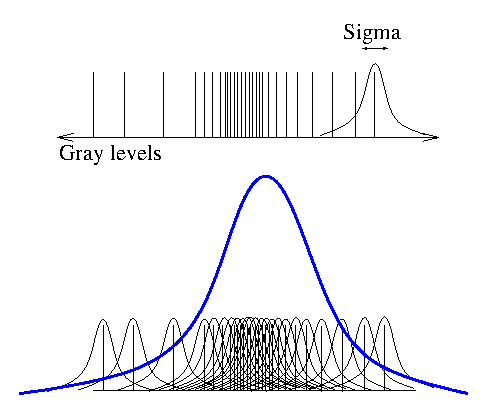
\includegraphics[width=0.48\textwidth]{ParzenWindowing13.eps}}

In a typical registration problem, direct access to the marginal 
and joint probability densities is not available and hence the
densities must be estimated from the image data. Parzen windows 
(also known as kernel density estimators) can be used for this purpose.
In this scheme, the densities are constructed by taking intensity 
samples $S$ from the image and super-positioning kernel functions 
$K(\cdot)$ centered on the elements of $S$ as illustrated in
Figure \ref{fig:ParzenWindowing}:

A variety of functions can be used as the smoothing kernel with the
requirement that they are smooth, symmetric, have zero mean and
integrate to one. For example, boxcar, Gaussian and B-spline functions are
suitable candidates.  A smoothing parameter is used to scale the kernel
function.  The larger the smoothing parameter, the wider the kernel function
used and hence the smoother the density estimate. If the parameter is too
large, features such as modes in the density will get smoothed out.  On the
other hand, if the smoothing parameter is too small, the resulting density
may be too noisy. The estimation is given by the following equation.

\begin{equation}
p(a) \approx P^{*}(a) = \frac{1}{N} \sum_{s_j \in S} K\left(a - s_j\right)
\end{equation}

Choosing the optimal smoothing parameter is a difficult research problem and
beyond the scope of this software guide.  Typically, the optimal value of the
smoothing parameter will depend on the data and the number of samples used.

\subsubsection{Viola and Wells Implementation}

OTB, through ITK, has multiple implementations of the mutual information
metric. One of the most commonly used is
\doxygen{itk}{MutualInformationImageToImageMetric} and follows the method specified
by Viola and Wells in \cite{Viola1997}.

\index{itk::Mutual\-Information\-Image\-To\-Image\-Metric}

In this implementation, two separate intensity samples $S$ and $R$ are drawn
from the image: the first to compute the density, and the second to approximate
the entropy as a sample mean:
\begin{equation}
H(A) = \frac{1}{N} \sum_{r_j \in R} \log P^{*}(r_j).
\end{equation}
Gaussian density is used as a smoothing kernel, where the standard deviation
$\sigma$ acts as the smoothing parameter.

\index{itk::Mutual\-Information\-Image\-To\-Image\-Metric!SetNumberOfSpatialSamples()}

The number of spatial samples used for computation is defined using
the \code{SetNumberOfSpatialSamples()} method. Typical values range from 50 to 100.
Note that computation involves an $N \times N$ loop and hence, the computation
burden becomes very expensive when a large number of samples is used.

\index{itk::Mutual\-Information\-Image\-To\-Image\-Metric!SetFixedImageStandardDeviation()}
\index{itk::Mutual\-Information\-Image\-To\-Image\-Metric!SetMovingImageStandardDeviation()}
The quality of the density estimates depends on the choice of the standard
deviation of the Gaussian kernel. The optimal choice will depend on the
content of the images.  In our experience with the toolkit, we have found
that a standard deviation of 0.4 works well for images that have been
normalized to have a mean of zero and standard deviation of 1.0. The standard
deviation of the fixed image and moving image kernel can be set separately
using methods
\code{SetFixedImageStandardDeviation()} and \code{SetMovingImageStandardDeviation()}.

\subsubsection{Mattes et al. Implementation}
Another form of mutual information metric available in ITK follows the method
specified by Mattes et al. in \cite{Mattes2001} and is implemented by the
\doxygen{itk}{MattesMutualInformationImageToImageMetric} class.

\index{itk::Mattes\-Mutual\-Information\-Image\-To\-Image\-Metric}
In this implementation, only one set of intensity samples is drawn from the
image.  Using this set, the marginal and joint probability density function
(PDF) is evaluated at discrete positions or bins uniformly spread within the
dynamic range of the images. Entropy values are then computed by summing over
the bins.

\index{itk::Mattes\-Mutual\-Information\-Image\-To\-Image\-Metric!SetNumberOfSpatialSamples()}
\index{itk::Mattes\-Mutual\-Information\-Image\-To\-Image\-Metric!SetNumberOfHistogramBins()}

The number of spatial samples used is set using method 
\code{SetNumberOfSpatialSamples()}. The number of bins used to compute
the entropy values is set via \code{SetNumberOfHistogramBins()}.

Since the fixed image PDF does not contribute to the metric derivatives, it
does not need to be smooth. Hence, a zero order (boxcar) B-spline kernel is
used for computing the PDF. On the other hand, to ensure smoothness, a third
order B-spline kernel is used to compute the moving image intensity PDF. The
advantage of using a B-spline kernel over a Gaussian kernel is that the
B-spline kernel has a finite support region. This is computationally
attractive, as each intensity sample only affects a small number of bins and
hence does not require a $N \times N$ loop to compute the metric value.

During the PDF calculations, the image intensity values are linearly scaled
to have a minimum of zero and maximum of one. This rescaling means that a
fixed B-spline kernel bandwidth of one can be used to handle image data with
arbitrary magnitude and dynamic range.


\subsection{Kullback-Leibler distance metric}
The \doxygen{itk}{KullbackLeiblerCompareHistogramImageToImageMetric} is yet another information based metric. 
Kullback-Leibler distance measures the relative entropy between two 
discrete probability distributions. The distributions are obtained from the 
histograms of the two input images, $A$ and $B$. 

The Kullback-Liebler distance between two histograms is given by
\begin{equation}
KL(A,B) =  \sum_i^N p_A(i) \times \log \frac{ p_A(i) }{p_B(i) }
\end{equation}

The distance is always non-negative and is zero only if the two distributions 
are the same. Note that the distance is not symmetric. In other 
words, $KL(A,B) \neq KL(B,A)$. Nevertheless, if the distributions are not too dissimilar, 
the difference between $KL(A,B)$ and $KL(B,A)$ is small.

The implementation in ITK is based on \cite{Chung2002}.

\subsection{Normalized Mutual Information Metric}
Given two images, $A$ and $B$, the normalized mutual information may be computed as 
\begin{equation}
NMI(A,B) = 1 + \frac{I(A,B)}{H(A,B)} = \frac{H(A) + H(B)}{H(A,B)}
\end{equation}
where the entropy of the images, $H(A)$, $H(B)$, the mutual 
information, $I(A,B)$ and the joint entropy $H(A,B)$ are computed as mentioned 
in \ref{sec:MutualInformationMetric}. Details of the implementation may be found in 
the \cite{Hajnal2001}.

\subsection{Mean Squares Histogram}
\index{itk::Mean\-Squares\-Histogram\-Image\-To\-Image\-Metric}

The \doxygen{itk}{MeanSquaresHistogramImageToImageMetric} is an alternative
implementation of the Mean Squares Metric. In this implementation the joint
histogram of the fixed and the mapped moving image is built first. The user
selects the number of bins to use in this joint histogram. Once the joint
histogram is computed, the bins are visited with an iterator. Given that each
bin is associated to a pair of intensities of the form: \{fixed intensity,
moving intensity\}, along with the number of pixels pairs in the images that
fell in this bin, it is then possible to compute the sum of square distances
between the intensities of both images at the quantization levels defined by
the joint histogram bins.

This metric can be represented with
Equation~\ref{eqn:MeanSquaresHistogramImageToImageMetric}

\begin{equation}
\label{eqn:MeanSquaresHistogramImageToImageMetric}
MSH = \sum_f \sum_m { H(f,m) { \left( f - m \right) } ^ 2 }
\end{equation}

where $H(f,m)$ is the count on the joint histogram bin identified with fixed image
intensity $f$ and moving image intensity $m$.


\subsection{Correlation Coefficient Histogram}
\index{itk::Correlation\-Coefficient\-Histogram\-Image\-To\-Image\-Metric}

The \doxygen{itk}{CorrelationCoefficientHistogramImageToImageMetric} computes the
cross correlation coefficient between the intensities in the fixed image and
the intensities on the mapped moving image. This metric is intended to be used
in images of the same modality where the relationship between the intensities
of the fixed image and the intensities on the moving images is given by a
linear equation. 

The correlation coefficient is computed from the Joint histogram as

\begin{equation}
\label{eqn:CorrelationCoefficientHistogramImageToImageMetric}
CC = \frac{ \sum_f \sum_m { \
            H(f,m) \left( f \cdot m - \
            \overline{f} \cdot \overline{m} \right)  } }{ \
            \sum_f { H(f) \left( (f - \overline{f})^2 \right) } \cdot \
            \sum_m { H(m) \left( (m - \overline{m})^2 \right) } }
\end{equation}

Where $H(f,m)$ is the joint histogram count for the bin identified with the
fixed image intensity $f$ and the moving image intensity $m$. The values
$\overline{f}$ and $\overline{m}$ are the mean values of the fixed and moving
images respectively.  $H(f)$ and $H(m)$ are the histogram counts of the fixed
and moving images respectively. The optimal value of the correlation
coefficient is $1$, which would indicate a perfect straight line in the
histogram.


\subsection{Cardinality Match Metric}
\index{itk::Match\-Cardinality\-Image\-To\-Image\-Metric}
The \doxygen{itk}{MatchCardinalityImageToImageMetric} computes cardinality of the
set of pixels that match exactly between the moving and fixed images. In other
words, it computes the number of pixel matches and mismatches between the two
images. The match is designed for label maps. All pixel mismatches are
considered equal whether they are between label 1 and label 2 or between label
1 and label 500. In other words, the magnitude of an individual label mismatch
is not relevant, or the occurrence of a label mismatch is important. 

The spatial correspondence between the fixed and moving images is established using 
a \doxygen{itk}{Transform} using the \code{SetTransform()} method and an interpolator 
using \code{SetInterpolator()}. Given that we are matching pixels with labels, 
it is advisable to use Nearest Neighbor interpolation.

\subsection{Kappa Statistics Metric}
\index{itk::Kappa\-Statistic\-Image\-To\-Image\-Metric}
The \doxygen{itk}{KappaStatisticImageToImageMetric} computes spatial intersection of 
two binary images. The metric here is designed for matching pixels in two images 
with the same exact value, which may be set using \code{SetForegroundValue()}. 
Given two images $A$ and $B$, the $\kappa$ coefficient is computed as
 
\begin{equation}
\kappa = \frac{|A| \cap |B|}{|A| + |B|}
\end{equation}

where $|A|$ is the number of foreground pixels in image $A$.  This computes the
fraction of area in the two images that is common to both the images. In the
computation of the metric, only foreground pixels are considered.

\subsection{Gradient Difference Metric}
\index{it::Gradient\-Difference\-Image\-To\-Image\-Metric}

This \doxygen{itk}{GradientDifferenceImageToImageMetric} metric evaluates the
difference in the derivatives of the moving and fixed images. The derivatives
are passed through a function $\frac{1}{1+x}$ and then they are added. The
purpose of this metric is to focus the registration on the edges of structures
in the images.  In this way the borders exert larger influence on the result
of the registration than do the inside of the homogeneous regions on the image.



%% \fi

%% % the clearpage command helps to avoid orphans in the title of the next
%% % section.
%% \clearpage

%% \section{Optimizers}
%% \label{sec:Optimizers}
%% \ifitkFullVersion
%% 
\index{itk::Optimizer}
\index{itk::Single\-Valued\-NonLinear\-Optimizer}


\begin{figure}
\center
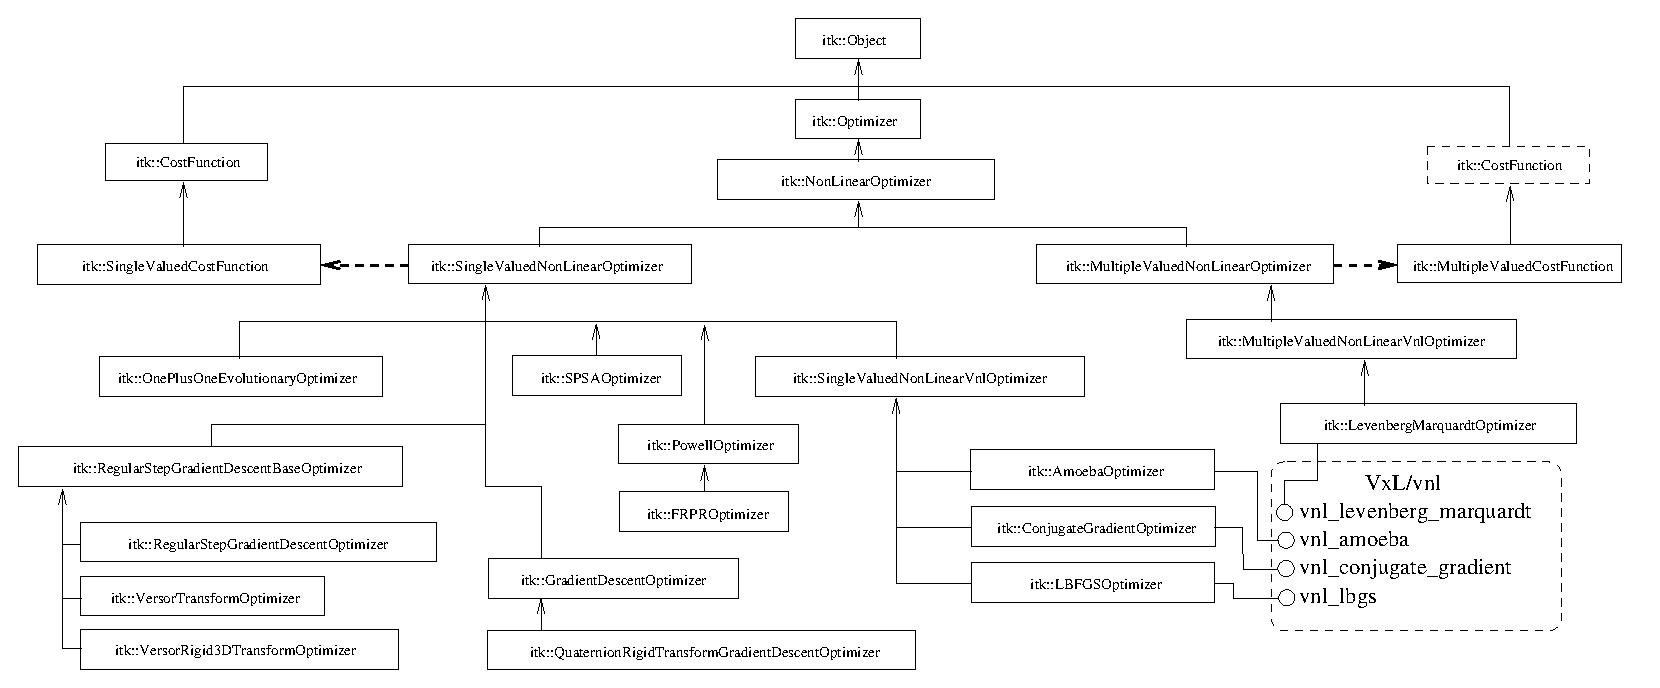
\includegraphics[width=\textheight,angle=270]{OptimizersHierarchy.eps}
\itkcaption[Class diagram of the Optimizer hierarchy]{Class diagram of the
optimizers hierarchy.}
\label{fig:OptimizersHierarchy}
\end{figure}

Optimization algorithms are encapsulated as \doxygen{itk}{Optimizer} objects
within OTB. Optimizers are generic and can be used for applications other than
registration.  Within the registration framework, subclasses of
\doxygen{itk}{SingleValuedNonLinearOptimizer} are used to optimize the metric
criterion with respect to the transform parameters.

\index{itk::Optimizer!SetInitialPosition()}
\index{itk::Optimizer!StartOptimization()}
\index{itk::Optimizer!GetCurrentPosition()}

The basic input to an optimizer is a cost function object. In the context
of registration, \doxygen{itk}{ImageToImageMetric} classes provides this functionality.
The initial parameters are set using \code{SetInitialPosition()} and
the optimization algorithm is invoked by \code{StartOptimization()}.
Once the optimization has finished, the final parameters can be obtained
using \code{GetCurrentPosition()}.

\index{itk::Optimizer!SetScales()}
Some optimizers also allow rescaling of their individual parameters. This is
convenient for normalizing parameters spaces where some parameters have
different dynamic ranges. For example, the first parameter of
\doxygen{itk}{Euler2DTransform} represents an angle while the last two parameters
represent translations. A unit change in angle has a much greater impact on an
image than a unit change in translation. This difference in scale appears as
long narrow valleys in the search space making the optimization problem more
difficult. Rescaling the translation parameters can help to fix this problem.
Scales are represented as an \doxygen{itk}{Array} of doubles and set defined using
\code{SetScales()}.

There are two main types of optimizers in OTB. In the first type we find
optimizers that are suitable for dealing with cost functions that return a
single value. These are indeed the most common type of cost functions, and are
known as \emph{Single Valued} functions, therefore the corresponding optimizers
are known as \emph{Single Valued} optimizers. The second type of optimizers are
those suitable for managing cost functions that return multiple values at each
evaluation. These cost functions are common in model-fitting problems and are
known as \emph{Multi Valued} or \emph{Multivariate} functions.  The
corresponding optimizers are therefore called \emph{MultipleValued} optimizers
in OTB.

The \doxygen{itk}{SingleValuedNonLinearOptimizer} is the base class for the first
type of optimizers while the \doxygen{itk}{MultipleValuedNonLinearOptimizer} is the
base class for the second type of optimizers.

The types of single valued optimizer currently available in OTB are:

\index{itk::Amoeba\-Optimizer}
\index{itk::Conjugate\-Gradient\-Optimizer}
\index{itk::Gradient\-Descent\-Optimizer}
\index{itk::Quaternion\-Rigid\-Transform\-Gradient\-Descent\-Optimizer}
\index{itk::LBFGS\-Optimizer}
\index{itk::LBFGSB\-Optimizer}
\index{itk::One\-Plus\-One\-Evolutionary\-Optimizer}
\index{itk::Powell\-Optimizer}
\index{itk::Regular\-Step\-Gradient\-Descent\-Optimizer}
\index{itk::SPSA\-Optimizer}
\index{itk::Versor\-Transform\-Optimizer}
\index{itk::Versor\-Rigid3D\-Transform\-Optimizer}
\index{itk::Levenberg\-Marquardt\-Optimizer}

\begin{itemize}

\item \textbf{Amoeba}: Nelder-Meade downhill simplex.  This optimizer is
actually implemented in the \code{vxl/vnl} numerics toolkit.  The ITK class
\doxygen{itk}{AmoebaOptimizer} is merely an adaptor class.

\item \textbf{Conjugate Gradient}: Fletcher-Reeves form 
of the conjugate gradient with or without preconditioning
(\doxygen{itk}{ConjugateGradientOptimizer}). It is also an adaptor to an optimizer in
\code{vnl}.

\item \textbf{Gradient Descent}: Advances parameters in the direction of the
gradient where the step size is governed by a learning rate
(\doxygen{itk}{GradientDescentOptimizer}). 

\item \textbf{Quaternion Rigid Transform Gradient Descent}: A specialized
version of GradientDescentOptimizer for QuaternionRigidTransform parameters,
where the parameters representing the quaternion are normalized to a magnitude
of one at each iteration to represent a pure rotation
(\doxygen{itk}{QuaternionRigidTransformGradientDescent}).

\item \textbf{LBFGS}: Limited memory Broyden, Fletcher, Goldfarb
and Shannon minimization. It is an adaptor to an optimizer in \code{vnl}
(\doxygen{itk}{LBFGSOptimizer}).

\item \textbf{LBFGSB}: A modified version of the LBFGS optimizer that allows to
specify bounds for the parameters in the search space.  It is an adaptor to an
optimizer in \code{netlib}. Details on this optimizer can be found
in~\cite{Byrd1995,Zhu1997} (\doxygen{itk}{LBFGSBOptimizer}).

\item \textbf{One Plus One Evolutionary}: Strategy that simulates the
biological evolution of a set of samples in the search space (\doxygen{itk}{OnePlusOneEvolutionaryOptimizer.}). Details on this optimizer can be
found in~\cite{Styner2000}.

\item \textbf{Regular Step Gradient Descent}: Advances parameters in the
direction of the gradient where a bipartition scheme is used to compute
the step size (\doxygen{itk}{RegularStepGradientDescentOptimizer}). 

\item \textbf{Powell Optimizer}: Powell optimization method.  For an
N-dimensional parameter space, each iteration minimizes(maximizes) the function
in N (initially orthogonal) directions. This optimizer is described
in~\cite{Press1992}.  (\doxygen{itk}{PowellOptimizer}).

\item \textbf{SPSA Optimizer}: Simultaneous Perturbation Stochastic
Approximation Method. This optimizer is described in
\url{http://www.jhuapl.edu/SPSA} and in~\cite{Spall1998}.
(\doxygen{itk}{SPSAOptimizer}). 

\item \textbf{Versor Transform Optimizer}: A specialized version of the 
RegularStepGradientDescentOptimizer for VersorTransform
parameters, where the current rotation is composed with the gradient rotation
to produce the new rotation versor. It follows the definition of versor
gradients defined by Hamilton~\cite{Hamilton1866}
(\doxygen{itk}{VersorTransformOptimizer}).

\item \textbf{Versor Rigid3D Transform Optimizer}: A specialized version of the
RegularStepGradientDescentOptimizer for VersorRigid3DTransform parameters,
where the current rotation is composed with the gradient rotation to produce
the new rotation versor. The translational part of the transform parameters are
updated as usually done in a vector space.
(\doxygen{itk}{VersorRigid3DTransformOptimizer}).


\end{itemize}

A parallel hierarchy exists for optimizing multiple-valued cost functions. The
base optimizer in this branch of the hierarchy is the
\doxygen{itk}{MultipleValuedNonLinearOptimizer} whose only current derived class
is:

\begin{itemize}

\item \textbf{Levenberg Marquardt}: Non-linear least squares minimization.
Adapted to an optimizer in \code{vnl} (\doxygen{itk}{LevenbergMarquardtOptimizer}).
This optimizer is described in~\cite{Press1992}.

\end{itemize}


Figure \ref{fig:OptimizersHierarchy} illustrates the full class hierarchy of
optimizers in OTB. Optimizers in the lower right corner are adaptor classes
to optimizers existing in the \code{vxl/vnl} numerics toolkit. The optimizers
interact with the \doxygen{itk}{CostFunction} class. In the registration framework
this cost function is reimplemented in the form of ImageToImageMetric.






%% \fi



%% \subsection{Registration using Match Cardinality metric}
%% \label{sec:RegistrationMatchCardinality}
%% \ifitkFullVersion
%% \input{ImageRegistration10.tex}
%% \fi


%% \subsection{Registration using the One plus One Evolutionary Optimizer}
%% \label{sec:RegistrationOnePlusOne}
%% \ifitkFullVersion
%% \input{ImageRegistration11.tex}
%% \fi



%% \subsection{Registration using masks constructed with Spatial objects}
%% \label{sec:RegistrationSpatialObjects}
%% \ifitkFullVersion
%% \input{ImageRegistration12.tex}
%% \fi



%% \subsection{Rigid registrations incorporating prior knowledge}
%% \label{sec:RegistrationCentered2DTransform}
%% \ifitkFullVersion
%% \input{ImageRegistration13.tex}
%% \fi


%% % the clearpage command helps to avoid orphans in the title of the next
%% % section.
%% \clearpage


%% \section{Image Pyramids}
%% \label{sec:ImagePyramids}
%% \ifitkFullVersion
%% \input{ImagePyramids.tex}
%% \fi


%% % the clearpage command helps to avoid orphans in the title of the next
%% % section.
%% \clearpage

%% \section{Deformable Registration}
%% \label{sec:DeformableRegistration}
%% \ifitkFullVersion
%% \input{DeformableRegistration.tex}
%% \fi

%% % the clearpage command helps to avoid orphans in the title of the next
%% % section.
%% \clearpage

%% \section{Demons Deformable Registration}
%% \label{sec:DemonsDeformableRegistration}
%% \ifitkFullVersion
%% \input{DemonsRegistration.tex}
%% \fi

%% \section{Visualizing Deformation fields}
%% \label{sec:VisualizingDeformationFields}
%% \ifitkFullVersion
%% \input{VisualizingDeformationFieldsUsingParaview.tex}
%% \fi

%% \ifitkFullVersion
%% \input{DeformableRegistration4OnBrain.tex}
%% \fi


%% % the clearpage command helps to avoid orphans in the title of the next
%% % section.
%% \clearpage



%% \section{Model Based Registration}
%% \label{sec:ModelBasedRegistration}
%% \ifitkFullVersion
%% \input{ModelBasedRegistration.tex}
%% \fi


%% \section{Point Set Registration}
%% \label{sec:PointSetRegistration}

%% PointSet-to-PointSet registration is a common problem in medical image
%% analysis. It usually arises in cases where landmarks are extracted from images
%% and are used for establishing the spatial correspondence between the images.
%% This type of registration can be considered to be the simplest case of
%% feature-based registration. In general terms, feature-based registration is
%% more efficient than the intensity based method that we have presented so far.
%% However, feature-base registration brings the new problem of identifying and
%% extracting the features from the images, which is not a minor challenge. 

%% The two most common scenarios in PointSet to PointSet registration are

%% \begin{itemize}
%% \item Two PointSets with the same number of points, and where each point in one
%% set has a known correspondence to exactly one point in the second set.
%% \item Two PointSets without known correspondences between the points of one set
%% and the points of the other. In this case the PointSets may have different
%% numbers of points.
%% \end{itemize}

%% The first case can be solved with a closed form solution when we are dealing
%% with a Rigid or an Affine Transform~\cite{Horn1987}. This is done in ITK with
%% the class \doxygen{LandmarkBasedTransformInitializer}. If we are interested in
%% a deformable Transformation then the problem can be solved with the
%% \doxygen{KernelTransform} family of classes, which includes Thin Plate Splines
%% among others~\cite{Rohr2001}. In both circumstances, the availability o f
%% correspondences between the points make possible to apply a straight forward
%% solution to the problem.


%% The classical algorithm for performing PointSet to PointSet registration is the
%% Iterative Closest Point (ICP) algorithm.  The following examples illustrate how
%% this can be used in ITK.



%% \subsection{Point Set Registration in 2D}
%% \label{sec:PointSetRegistrationIn2D}

%% \ifitkFullVersion
%% \input{IterativeClosestPoint1.tex}
%% \fi




%% \subsection{Point Set Registration in 3D}
%% \label{sec:PointSetRegistrationIn3D}

%% \ifitkFullVersion
%% \input{IterativeClosestPoint2.tex}
%% \fi



%% \subsection{Point Set to Distance Map Metric}
%% \label{sec:PointSetToDistanceMapMetric}

%% \ifitkFullVersion
%% \input{IterativeClosestPoint3.tex}
%% \fi



%% \section{Registration Troubleshooting}
%% So you read the previous sections, you wrote the code, it compiles and links fine,
%% but when you run it the registration results are not what you were expecting.
%% In that case, this section is for you. This is a compilation of the most common
%% problems that users face when performing image registration. It provides explanations
%% on the potential sources of the problems, and advice on how to deal with those problems.

%% Most of the material in this section has been taken from frequently asked questions of 
%% the ITK users list.


%% \subsection{Too many samples outside moving image buffer}


%% http://public.kitware.com/pipermail/insight-users/2007-March/021442.html

%% This is a common error message in image registration.

%% It means that at the current iteration of the optimization,
%% the two images as so off-registration that their spatial
%% overlap is not large enough for bringing them back into
%% registration.

%% The common causes of this problem are:

%% \begin{itemize}
%% \item Poor initialization:    You must initialize the transform properly.
%% Please read the ITK Software Guide http://www.itk.org/ItkSoftwareGuide.pdf  for
%% a description of the use of the CenteredTransformInitializer class.
%% \item Optimzer steps too large. If you optimizer takes steps that are too
%% large, it risks to become unstable and to send the images too far appart.  You
%% may want to start the optimizer with a maximum step lenght of 1.0, and only
%% increase it once you have managed to fine tune all other registration
%% parameters.

%% Increasing the step length makes your program faster, but it also makes it more
%% unstable.



%% \item Poor set up o the transform parameters scaling.  This is extremely
%% critical in registration. You must make sure that you balance the relative
%% difference of scale between the rotation parameters and the translation
%% parameters.

%% In typical medical datasets such as CT and MR, translations are measured in
%% millimeters, and therefore are in the range of -100:100, while rotations are
%% measured in radians, and therefore they tend to be in the range of   -1:1.


%% A rotation of 3 radians is catastrophic, while a translation of 3 millimeters
%% is rather inoffensive.  That difference in scale is the one that must be
%% accounted for.  
%% \end{itemize}



%% \subsection{General heuristics for parameter fine-tunning}





%% http://public.kitware.com/pipermail/insight-users/2007-March/021435.html

%% Here is some advice on how to fine tune the parameters
%% of the registration process.


%% 1) Set Maximum step length to 0.1 and do not change it
%%    until all other parameters are stable.

%% 2) Set Minimum step length to 0.001 and do not change it.

%%    You could interpret these two parameters as if their
%%    units were radians. So, 0.1 radian = 5.7 degrees.


%% 3) Number of histogram bins:

%%     First plot the histogram of your image using the
%%     example program in

%%     Insight/Examples/Statistics/ImageHistogram2.cxx

%%     In that program use first a large number  of bins
%%     (for example 2000) and identify the different
%%     populations of intensity level and to what anatomical
%%     structures they correspond.

%%     Once you identify the anatomical structures in the
%%     histogram, then rerun that same program with less
%%     and less number of bins, until you reach the minimun
%%     number of bins for which all the tissues that are important
%%     for your application, are still distinctly differentiated in the
%%     histogram.  At that point, take that number of bins and
%%     us it for your Mutual Information metric.


%% 4)  Number of Samples:
%%     The trade-off with the number of samples is the following:

%%     a) computation time of registration is linearly proportional
%%        to the number of samples
%%                                                                                                                         b) the samples must be enough to significantly populate
%%                                                                                                                            the joint histogram.
%%                                                                                                                         c) Once the histogram is populated, there is not much
%%                                                                                                                            use in adding more samples.
%% Therefore do the following:

%% Plot the joint histogram of both images, using the number
%% of bins that you selected in item (3). You can do this by
%% modifying the code of the example:

%% Insight/Examples/Statistics/
%% ImageMutualInformation1.cxx
%% you have to change the code to print out the values
%% of the bins. Then use a plotting program such as gnuplot,
%% or Matlab, or even Excel and look at the distribution.
%% The number of samples to take must be enough
%% for producing the same "appearance" of the joint histogram.
%% As an arbitrary rule of thumb you may want to start using
%% a high number of samples (80% ~ 100%). And do not
%% change it until you have mastered the other parameters
%% of the registration.  Once you get your registration to converge
%% you can revisit the number of samples and reduce it in order
%% to make the registration run faster. You can simply reduce it
%% until you find that the registration becomes unstable. That's
%% your critical bound for the minimum number of samples.
%% Take that number and multiply it by the magic number 1.5,
%% to send it back to a stable region, or if your application is
%% really critical, then use an even higher magic number x2.0.

%% This is just engineering: you figure out what is the minimal
%% size of a piece of steel that will support a bridge, and then
%% you enlarge it to keep it away from the critical value.

%% 5)  The MOST critical values of the registration process are the
%% scaling parameters that define the proportions between
%% the parameters of the transform. In your case, for an Affine
%% Transform in 2D, you have 6 parameters. The first four are
%% the ones of the Matrix, and the last two are the translation.
%% The rotation matrix value must be in the ranges of radians
%% which is typically [ -1 to 1 ], while the translation values are
%% in the ranges of millimeters (your image size units).
%% You want to start by setting the scaling of the matrix
%% parameters to 1.0, and the scaling of the Translation
%% parameters to the holy esoteric values:

%% 1.0   /  (  10.0 * pixelspacing[0]  *  imagesize[0]  )
%% 1.0   /  (  10.0 * pixelspacing[1]  *  imagesize[1]  )

%% This is telling the optimizer that you consider that rotating
%% the image by 57 degrees is as "significant" as translating
%% the image by half its physical extent.

%% Note that esoteric value has included the arbitrary number
%% 10.0 in the denominator, for no other reason that we have
%% been lucky when using that factor. This of course is just a
%% supersticion, so you should feel free to experiment with
%% different values of this number.

%% Just keep in mind that what the optimizer will do is to
%% "jump" in a paramteric space of 6 dimension, and that the
%% component of the jump on every dimension will be proporitional
%% to 1/scaling factor * OptimizerStepLenght.     Since you put
%% the optimizer Step Length to 0.1, then the optimizer will start
%% by exploring the rotations at jumps of about 5degrees, which
%% is a conservative rotation for most medical applications.

%% If you have reasons to think that your rotations are larger or
%% smaller, then you should modify the scaling factor of the  matrix
%% parameters accordingly.

%% In the same way, if you thinkl that 1/10 of the image size is too
%% large as the first step for exploring the translations, then you
%% should modify the scaling of  translation parameters accordingly.



%% In order to drive all these you need to analyze the feedback that
%% the observer is providing you. For example, plot the metric values,
%% and plot the translation coordinates so that you can get a feeling
%% of how the registration is behaving.


%% Note also that image registration is not a science. it is a pure
%% engineerig practice, and therefore, there are no correct answers,
%% nor "truths" to be found. It is all about how much quality your want,
%% and how must computation time, and development time are you
%% willing to pay for that quality. The "satisfying" answer for your
%% specific application must be found by exploring the trade-offs
%% between the different parameters that regulate the image
%% registration process.

%% If you are proficient in VTK you may want to consider attaching
%% some visualization to the Event observer, so that you can have
%% a visual feedback on the progress of the registration. This is a
%% lot more productive than trying to interpret the values printed
%% out on the console by the observer.




\chapter{Disparity Map Estimation}


This chapter introduces the tools available in OTB for the estimation
of geometric disparities between images.


\section{Disparity Maps}
\ifitkFullVersion
\label{sec:DisparityMaps}
\fi

The problem we want to deal with is the one of the
automatic disparity map estimation of images acquired with different sensors. By different
sensors, we mean sensors which produce images with different
radiometric properties, that is, sensors which measure different
physical magnitudes: optical sensors operating in different spectral
bands, radar and optical sensors, etc.\\

For this kind of image pairs, the classical approach of fine
correlation \cite{correl1,correl2}, can not always be used to
provide the required accuracy, since this similarity measure (the correlation
coefficient) can only measure similarities up to an affine
transformation of the radiometries.\\

There are two main questions which can be asked about what we want to
do:
\begin{enumerate}
\item Can we define what the similarity is between, for instance, a radar
and an optical image?
\item What does {\em fine registration} mean in the case where the
geometric distortions are so big and the source of information can be
located in different places (for instance, the same edge can be
produced by the edge of the roof of a building in an optical image and
by the wall-ground bounce in a radar image)?
\end{enumerate}

We can answer by saying that the images of the same object obtained by different
sensors are two different representations of the same reality. For the
same spatial location, we have two different measures. Both informations
come from the same source and thus they have a lot of common
information. This relationship may not be perfect, but it can be
evaluated in a relative way: different geometrical distortions are
compared and the one leading to the strongest link between the two
measures is kept.\\

%% proposed by Ventura et al. \cite{ventura}. They even applied it to the
%% problem of image to map registration. The approach was also finding HP
%% by matching extracted features.\\


%% Dai and Khorram \cite{xiaolong} use a feature based approach: they
%% extract closed edges which are characterized using invariant
%% moments. Then, the extracted areas are matched using their
%% characterization. Finally, the centers of gravity of each area are
%% used as HP for the estimation of an affine transformation. They apply
%% the approach to Landsat images and they obtain an accuracy better than
%% one pixel, which is similar to the accuracy obtained with manual registration.\\

%% Djamdji et al. \cite{djamdji} propose a multiresolution approach where
%% the discrete wavelet transform is used. The automatic extraction of
%% HP is done by comparing thresholded wavelet coefficients.\\

%% All these approaches try to extract HP in order to
%% compute an analytical deformation model. On the other hand,
When
working with images acquired with the same (type of) sensor one can
use a very effective approach. Since a correlation coefficient measure
is robust and fast for similar images, one can afford to apply it in
every pixel of one image in order to search for the corresponding
HP in the other image. One can thus build a deformation
grid (a sampling of the deformation map). If the sampling step of this grid is short enough, the
interpolation using an analytical model is not needed and high
frequency deformations can be estimated. The obtained grid can be used
as a re-sampling grid and thus obtain the registered images.\\

No doubt, this approach, combined with image interpolation techniques
(in order to estimate sub-pixel deformations) and multi-resolution
strategies allows for obtaining the best performances in terms of
deformation estimation, and hence for the automatic image
registration.\\

Unfortunately, in the multi-sensor case, the correlation coefficient
can not be used. We will thus try to find similarity measures which can be
applied in the multi-sensor case with the same approach as the
correlation coefficient.\\

%% \section{Model for the image registration problem\label{model}}
%% In this section,
We start by giving several definitions which allow for the
formalization of the image registration problem. First of all, we
define the master image and the slave image:
\begin{defin}
Master image: image to which other images will be registered; its
geometry is considered as the reference.
\end{defin}

\begin{defin}
Slave image: image to be geometrically transformed in order to be
registered to the master image.
\end{defin}

Two main concepts are the one of {\em similarity measure} and the one
of {\em geometric transformation}:
\begin{defin}
\label{def-simil}Let $I$ and $J$ be two images and let $c$ a similarity
criterion, we call similarity measure any scalar, strictly positive function 
\begin{equation}
S_c(I,J) = f(I,J,c).
\end{equation}

$S_c$ has an absolute maximum when the two images $I$ and $J$
are {\it identical} in the sense of the criterion $c$.\\
\end{defin}

\begin{defin}\label{defin-T}
A geometric transformation $T$ is an operator which, applied to the
coordinates $(x,y)$ of a point in the slave image, gives the
coordinates $(u,v)$ of its HP in the master image:

\begin{equation}
\left( \begin{array}{c}
u\\
v\\
\end{array}\right) = T \left( \begin{array}{c}
x\\
y\\
\end{array}\right)
\label{Tgeom}
\end{equation}

\end{defin}

Finally we introduce a definition for the image registration problem:
\begin{defin}\label{defin-recal}
Registration problem: \begin{enumerate}
\item determine a geometric transformation $T$ which maximizes the
similarity between a master image $I$ and the result of the
transformation $T\circ J$:
\begin{equation}
Arg \max_T(S_c(I,T\circ J));
\end{equation}
\item re-sampling of $J$ by applying $T$.
\end{enumerate}

\end{defin}

%% We must note that Le Moigne et al. have proposed in a recent contribution
%% \cite{ig02lemoigne} a modular approach for the
%% registration which allows the analysis of different similarity
%% measures and different optimization strategies. The presented results,
%% which are still preliminary, are very promising. The multi-sensor
%% case has been dealt with, but only for optical images (Ikonos and
%% Landsat/ETM+). The case of very different images (for instance optical
%% and radar) has not been explored.\\


\subsection{Geometric deformation modeling\label{sec-model}}
The geometric transformation of definition \ref{defin-T} is used for
the correction of the existing deformation between the two images to be
registered. This deformation contains informations which are linked to
the observed scene and the acquisition conditions. They
can be classified into 3 classes depending on their physical source:
\begin{enumerate}
\item deformations linked to the mean attitude of the sensor
(incidence angle, presence or absence of yaw steering, etc.);
\item deformations linked to a stereo vision (mainly due to the topography);
\item deformations linked to attitude evolution during the acquisition
(vibrations which are mainly present in push-broom sensors).
\end{enumerate}

These deformations are characterized by their spatial frequencies and
intensities which are summarized in table \ref{tab-deform}.\\

\begin{table}[b]
\begin{center}
\begin{tabular}{|c|c|c|}
\hlx{hv}
& Intensity & Spatial Frequency\\
\hlx{hv}
Mean Attitude & Strong & Low \\
\hlx{hv}
Stereo & Medium & High and Medium\\
\hlx{hv}
Attitude evolution & Low & Low to Medium \\
\hlx{vhs}
\end{tabular}
\end{center}
\caption{Characterization of the geometric deformation sources}
\label{tab-deform}
\end{table}

Depending on the type of deformation to be corrected, its model will be
different. For example, if the only deformation to be corrected is the
one introduced by the mean attitude, a physical model for the
acquisition geometry (independent of the image contents) will be
enough. If the sensor is not well known, this deformation can be
approximated by a simple analytical model. When the deformations to be
modeled are high frequency, analytical (parametric) models are not
suitable for a fine registration. In this case, one has to use a fine
sampling of the deformation, that means the use of deformation
grids. These grids give, for a set of pixels of the master image,
their location in the slave image.\\

The following points summarize the problem of the deformation modeling:
\begin{enumerate}
\item An analytical model is just an approximation of the
deformation. It is often obtained as follows:
\begin{enumerate}
\item Directly from a physical model without using any image content information.
\item By estimation of the parameters of an a priori model
(polynomial, affine, etc.). These parameters can be estimated:
\begin{enumerate}
\item Either by solving the equations obtained by taking HP. The HP can be manually or automatically extracted.
\item Or by maximization of a global similarity measure.
\end{enumerate}

\end{enumerate}
\item A deformation grid is a sampling of the deformation map.
\end{enumerate}

The last point implies that the sampling period of the grid must be short
enough in order to account for high frequency deformations (Shannon
theorem). Of course, if the deformations are non stationary (it is
usually the case of topographic deformations), the sampling can 
be irregular.\\

As a conclusion, we can say that definition \ref{defin-recal} poses
the registration problem as an optimization problem. This optimization
can be either global or local with a similarity measure which can also
be either local or global. All this is synthesized in table  \ref{tab-approches}.\\

\begin{table}[b]
\begin{center}
\begin{tabular}{|c|c|c|}
\hlx{hv}
Geometric model & Similarity measure & Optimization of the \\
& & deformation \\
\hlx{hv}
Physical model & None & Global \\
\hlx{hv}
Analytical model  & Local & Global \\
with a priori HP & & \\
\hlx{hv}
Analytical model& Global & Global \\
without a priori HP & & \\
\hlx{hv}
Grid & Local & Local \\
\hlx{vhs}
\end{tabular}
\end{center}
\caption{Approaches to image registration}
\label{tab-approches}
\end{table}

The ideal approach would consist in a registration which is locally
optimized, both in similarity and deformation, in order to have the
best registration quality. This is the case when deformation grids with
dense sampling are used. Unfortunately, this case is the most
computationally heavy and one often uses either a low sampling rate of
the grid, or the evaluation of the similarity in a small set of pixels
for the estimation of an analytical model. Both of these choices lead to local registration
errors which, depending on the topography, can amount several
pixels.\\

Even if this registration accuracy can be enough in many
applications, (ortho-registration, import into a GIS, etc.), it is not
acceptable in the case of data fusion, multi-channel segmentation or
change detection \cite{townshend}. This is why we will focus on the
problem of deformation estimation using dense grids.\\

%% None of the references presented in section \ref{review} uses the
%% local optimization approach. We can also note that in the multi-sensor
%% case only few authors \cite{ig02lemoigne} have used any similarity
%% measure other than the correlation coefficient. However, in the
%% medical imaging field, as we will see in section \ref{sec-simil}, a
%% lot of similarity measures have been proposed as a generalization of
%% the correlation coefficient. These measures enable the registration of
%% very different imagery modalities. Nevertheless, these works are not
%% directly usable in our problem since the geometric deformations
%% present in medical images can be easily represented by global
%% analytical models. Indeed, often a rigid model (rotation, translation,
%% scale) or slightly elastic (affine plus a $a\cdot x\cdot y$ term) is
%% enough since the sensors are stable, the stereo effect is small and
%% only the point of view changes. As we have noted above, deformations
%% due to topography can locally have high frequencies for medium and
%% high resolution sensors (30 m. and better), thus our need for a fine
%% modeling. We also point out that the problem of hidden faces is beyond
%% the scope of this paper.\\


\subsection{Similarity measures\label{sec-simil}}


The fine modeling of the geometric deformation we are looking for
needs for the estimation of the coordinates of nearly every pixel in
the master image inside the slave image. In the classical mono-sensor
case where we use the correlation coefficient we proceed as follows.\\

The geometric deformation is modeled by local rigid displacements. One
wants to estimate the coordinates of each pixel of the master image inside the
slave image. This can be represented by a displacement vector
associated to every pixel of the master image. Each of the two components
(lines and columns) of this vector field will be called deformation grid.\\

We use a small window taken in the master image and we test the similarity
for every possible shift within an exploration area inside the slave
image (figure \ref{zones}). \\

\begin{figure}
\begin{center}{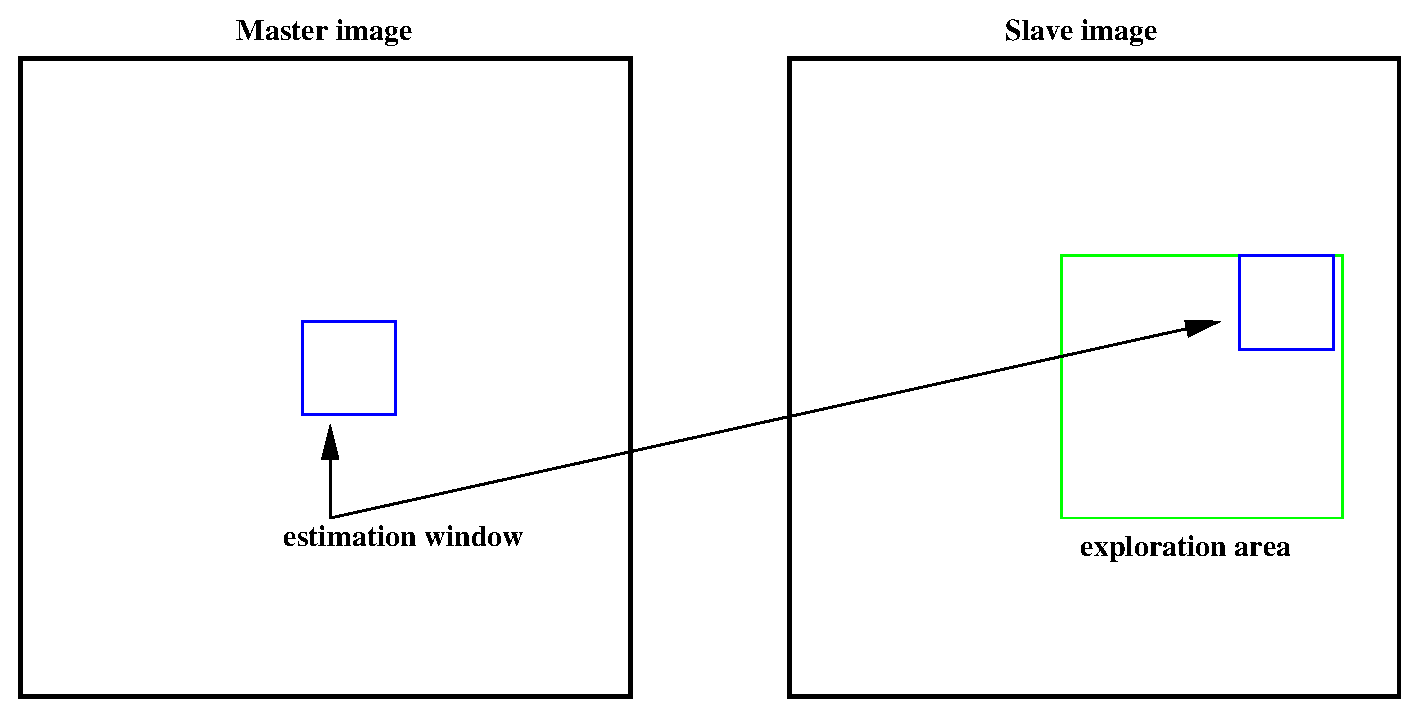
\includegraphics[width=0.8\hsize]{zones.eps}}
\caption{Estimation of the correlation surface.}
\label{zones}
\end{center}\end{figure}


That means that for each position we compute the correlation
coefficient. The result is a correlation surface whose
maximum gives the most likely local shift between both images:

\begin{equation}
\begin{split}
&\rho_{I,J}(\Delta x, \Delta y) = \\
&\frac{1}{N}\frac{\sum_{x,y}(I(x,y)-m_I)(J(x+\Delta x,y+\Delta y)-m_J)}{\sigma_I
\sigma_J}.
\end{split}
\end{equation}

In this expression, $N$ is the number of pixels of the analysis
window, $m_I$ and $m_J$ are the estimated mean values inside the
analysis window of respectively image $I$ and image $J$ and $\sigma_I$
and $\sigma_J$ are their standard deviations.\\

Quality criteria can be applied to the estimated maximum in order to
 give a confidence factor to the estimated shift: width of the peak,
 maximum value, etc. Sub-pixel shifts can be measured by applying
 fractional shifts to the sliding window. This can be done by image interpolation.\\

The interesting parameters of the procedure are:
\begin{itemize}
\item The size of the exploration area: it determines the
computational load of the algorithm (we want to reduce it), but it has
to be large enough in order to cope with large deformations.
\item The size of the sliding window: the robustness of the correlation
coefficient estimation increases with the window size, but the
hypothesis of local rigid shifts may not be valid for large windows.
\end{itemize}

The correlation coefficient cannot be used with original grey-level
images in the multi-sensor case. It could be used on extracted
features (edges, etc.), but the feature extraction can introduce
localization errors. Also, when the images come from sensors using
very different modalities, it can be difficult to find similar
features in both images. In this case, one can try to find the
similarity at the pixel level, but with other similarity measures and
apply the same approach as we have just described.\\

The concept of similarity measure has been presented in definition
\ref{def-simil}. The difficulty of the procedure lies in finding the
function $f$ which properly represents the criterion $c$. We also need
that $f$ be easily and robustly estimated with small windows. We extend here what we proposed in \cite{ig02simil}.\\

\subsection{The correlation coefficient\label{expe}}
We remind here the computation of the correlation coefficient between
two image windows $I$ and $J$. The coordinates of the pixels inside
the windows are represented by $(x,y)$:

\begin{equation}
\rho(I,J) = \frac{1}{N}\frac{\sum_{x,y}(I(x,y)-m_I)(J(x,y)-m_J)}{\sigma_I
\sigma_J}.
\label{coeffcorr}
\end{equation}

In order to qualitatively characterize the different similarity
measures we propose the following experiment. We take two images which
are perfectly registered and we extract a small window
of size $N\times M$ from each of the images (this size is set to
$101\times 101$ for this experiment). For the master image, the
window will be centered on coordinates $(x_0,
y_0)$ (the center of the image) and for the slave image, it will be centered on coordinates $(x_0+\Delta x,
y_0)$. With different values of $\Delta x$ (from -10 pixels to 10
pixels in our experiments), we obtain an estimate of $\rho(I,J)$ as a
function of $\Delta x$, which we write as
$\rho(\Delta x)$ for short. The obtained curve should have a maximum for
$\Delta x =0$, since the images are perfectly registered. We would
also like to have an absolute maximum with a high value and with a
sharp peak, in order to have a good precision for the shift estimate.\\

%% In the following, we will make this experiment with different image
%% pairs and different similarity measures. Figure \ref{fig-correl}
%% shows the results obtained when the correlation coefficient is applied
%%  to (\ref{correl-B1B1}) one extract of the B1 channel of a Spot 5
%% image with itself, (\ref{correl-B1B3}) an extract of channel B1 with the
%% extract of channel B3,  and (\ref{correl-B1ERS}) the extract of
%% channel B1 with an
%% extract of an ERS-2 SAR image. The images are presented in figures
%% \ref{histo_b1_b1}, \ref{histo_b1_b3} and \ref{histo_b1_ers}.\\


%% % \begin{figure*}
%% % \centerline{\subfigure[Correlation B1-B1]{\includegraphics[width=0.5\hsize]{CORREL_b1_b1_10.pdf}\label{correl-B1B1}} \\
%% % \subfigure[Correlation
%% % B1-B3]{\includegraphics[width=0.5\hsize]{CORREL_b1_b3_10.pdf}\label{correl-B1B3}}\\
%% % \subfigure[Correlation B1-ERS]{\includegraphics[width=0.5\hsize]{CORREL_b1_ERS_10_0.pdf}\label{correl-B1ERS}}}
%% % \caption{Measure of $\rho(\Delta x)$ for 3 different pairs of images.}
%% % \label{fig-correl}
%% % \end{figure*}

%% \begin{figure*}
%% \centering
%% \subfigure[Correlation B1-B1]{\includegraphics[width=0.4\hsize]{CORREL_b1_b1_10.pdf}\label{correl-B1B1}} \\
%% \subfigure[Correlation
%% B1-B3]{\includegraphics[width=0.4\hsize]{CORREL_b1_b3_10.pdf}\label{correl-B1B3}}\\
%% \subfigure[Correlation B1-ERS]{\includegraphics[width=0.4\hsize]{CORREL_b1_ERS_10_0.pdf}\label{correl-B1ERS}}
%% \caption{Measure of $\rho(\Delta x)$ for 3 different pairs of images.}
%% \label{fig-correl}
%% \end{figure*}

%% We can see that the correlation coefficient has a good behavior for
%% the first pair, but its performances are bad when the images
%% radiometries are different. The correlation coefficient
%%  can be characterized as follows:
%% \begin{itemize}
%% \item Well known algorithm.
%% \item Fits the registration needs when using radiometrically similar images.
%% \item Simple and fast computation.
%% \item High precision in the estimation of the deformation.
%% \item Robust to noise.
%% \end{itemize}

%% However its main disadvantage is that it can only take into account
%%  affine transformations between radiometries ($j = \alpha i + \beta$)
%%  so it can not be used in the general multi-sensor case.\\


%% \subsection{Generalization: probabilistic interpretation \label{sec_correl}}
%% The correlation coefficient formulation (equation \ref{coeffcorr}) can
%% be revisited with a probabilistic interpretation:

%% \begin{equation}
%% \begin{split}
%% \rho(I,J) &= \frac{1}{N}\frac{\sum_{x,y}(I(x,y)-m_I)(J(x,y)-m_J)}{\sigma_I
%% \sigma_J} \\
%% &= \sum_{(i,j)}\frac{(i-m_I)(j-m_J)}{\sigma_I \sigma_J}p_{ij}
%% \end{split}
%% \label{coeffcorr2}
%% \end{equation}

%% where the sum is taken over the list of radiometry pairs $(i,j)$, and
%% $p_{ij}$ is the value of the joint normalized histogram (estimation of
%% the joint probability density function, pdf, $f_{ij}(i,j)$) of the pair of images.\\

%% That means that we are assuming a linear model
%% \begin{equation}
%% j = (i-m_I)\frac{\sigma_J}{\sigma_I}+m_J,
%% \end{equation}
%% and we evaluate its likelihood by weighting with the probability of
%% each radiometry couple, $p_{ij}$.\\

%% One could assume different models for the radiometry pairs leading to
%% different measures as, for instance, the identity model , $i=j$, which
%% leads to the $L_n$ norm:

%% \begin{equation}
%% L_n(I,J) = \sum_{i,j} \left| i - j\right|^n p_{ij},
%% \end{equation}

%% or more complex models based on textural approaches :

%% Diagonal moment:
%% \begin{equation}
%% MD(I,J) = \sum_{i,j}\left| i - j\right|(i+j-\sigma_I-\sigma_J) p_{ij},
%% \end{equation}

%%  Cluster Shade:
%% \begin{equation}
%% C_{shade}(I,J) = \sum_{i,j} (i+j-\sigma_I-\sigma_J)^3 p_{ij},
%% \end{equation}

%%  Cluster Prominence:
%% \begin{equation}
%% C_{pro}(I,J) = \sum_{i,j} (i+j-\sigma_I-\sigma_J)^4 p_{ij}.
%% \end{equation}

%% An assessment of these measures for image registration can be found in
%% \cite{bro}. They are very sensitive to noise and are not useful for
%% the comparison of grey-levels of multi-sensor image pairs.\\

%% \subsection{Estimation of similarity measures and $p_{IJ}$}

%% In the expression of the correlation coefficient the term $p_{ij}$ is
%% an estimation of the joint pdf of the radiometries of
%% the images we are comparing. It can be seen as a link (transfer
%% function) between both radiometries.\\

%% % We want a measure of the
%% % similarity measure which is valid locally, that is, which takes into
%% % account the specificities of the neighborhood of the pixel for which
%% % we are estimating the deformation. That means that we have to use a
%% % small estimation window around the pixel of interest. On the other
%% % hand, we want a robust estimate, thus we need reliable values of
%% % $p_{ij}$, which means the use of a high number of samples.\\


%% %\subsubsection{Examples of $p_{ij}$ estimation}

%% We show here several examples of the estimation of the joint
%% histogram. On figures \ref{histo_b1_b1}, \ref{histo_b1_b3} and
%% \ref{histo_b1_ers} are shown respectively the joint histograms of one
%% image with itself (B1-B1), two different channels of the same Spot 5
%% image (B1-B3) and a Spot 5 B3 - ERS-2 pair.\\

%% \begin{figure}
%% \centering
%% \subfigure[SPOT 5 B1]{\includegraphics[width=0.5\hsize]{b1_1980_1980.pdf}} \\
%% \subfigure[Joint histogram]{\includegraphics[width=0.5\hsize]{hb1.pdf}}
%% \caption{Joint histogram of an image with itself.}
%% \label{histo_b1_b1}
%% \end{figure}


%% \begin{figure}
%% \centering
%% \subfigure[SPOT 5 B1]{\includegraphics[width=0.5\hsize]{b1_3376_3882.pdf}}\\
%% \subfigure[SPOT 5 B3]{\includegraphics[width=0.5\hsize]{b3_3376_3882.pdf}}\\
%% \subfigure[Joint histogram]{\includegraphics[width=0.5\hsize]{hb3.pdf}}\\
%% \caption{Joint histogram of two channels (B1-B3) of the same Spot 5 image.}
%% \label{histo_b1_b3}
%% \end{figure}



%% \begin{figure}
%% \centering
%% \subfigure[SPOT 5 B3]{\includegraphics[width=0.5\hsize]{b1_1500_2500.pdf}}\\
%% \subfigure[ERS-2]{\includegraphics[width=0.5\hsize]{ERS_1500_2500.pdf}}\\
%% \subfigure[Joint histogram]{\includegraphics[width=0.5\hsize]{hers.pdf}}\\
%% \caption{Joint histogram of a Spot 5 B3 image and a ERS-2 image.}
%% \label{histo_b1_ers}
%% \end{figure}

%% As expected, the joint histogram of an image with itself is a straight
%% line with slope 1. It shows the full correlation between the two
%% images: the identity transfer function. This kind of situation is well
%% dealt with by the correlation coefficient.\\

%% The B1-B3 case (figure \ref{histo_b1_b3}) shows two nearly linear tendencies which are
%% mixed up. This case can not be dealt with by the correlation coefficient.\\

%% Finally, figure \ref{histo_b1_ers} shows the impossibility of finding
%% any correlation link between two sensors which are as different as an
%% optical and a radar one.\\


%% \subsubsection{Computation time}
%% The main difference between the two expressions of the correlation
%% coefficient given by equations \ref{coeffcorr} and \ref{coeffcorr2} is
%% the estimation of the joint pdf needed in the second
%% expression. This estimation is usually done by computing the joint
%% histogram. The joint histogram can be computed with different methods,
%% but their discussion is beyond the scope of this paper. However it is
%% important to note that the method chosen for histogram computation may
%% induce significative changes in the computation cost of the similarity
%% measure. As an example, with our implementation (counting with
%% optimization of the number of classes) there is an increase factor of 4 in
%% computation time between equation \ref{coeffcorr} and equation
%% \ref{coeffcorr2}.\\

%% The multi-sensor measures which will be introduced in the next section
%% need the estimation of the joint histogram. Hence, their computation
%% time is comparable to the one of equation \ref{coeffcorr2}. The
%% differences of computation complexity between these measures are
%% negligible, since the longest part of the algorithm is taken by the
%% joint histogram estimation.\\


%% \subsection{Multi-sensor measures.}
%% We introduce here several similarity measures which have been proved
%% useful in the problem of multi-modality medical image registration \cite{dsarrut-thesis}.\\

%% In the following, the sums will be computed over radiometry values. We
%% will use the conditional mean:
%% \begin{equation}
%% m_{I|j} = \frac{1}{p_j}\sum_i i p_{ij};
%% \end{equation}

%% and the conditional variance:

%% \begin{equation}
%% \sigma^2_{I|j} = \frac{1}{p_j}\sum_i (i-m_{I|j})^2 p_{ij}.
%% \end{equation}

%% For each of the following measures, we will perform the experiment
%% described in section \ref{expe}.\\


%% \subsubsection{Measures using the radiometry values and the probabilities}

%% Within this class, we will not take into account the measures which
%% are based on the differences of radiometries ($L_n$ norm of the
%% difference) \cite{tru98,cm87,akn89}, or textural measures, since they
%% give low quality results.\\


%% \paragraph{Normalised standard deviation or Woods criterion}

%% The work by Woods et al. first on mono-modal registration 
%% \cite{wcm92} and then on multi-modal registration \cite{wmc93} lead to
%% the elaboration of this similarity measure. Given the intensity on one
%% image, that is the set of pixels having this value, this measure takes
%% into account the variability of the intensities of the homologous
%% pixels in the other image. The underlying hypothesis is that this
%% variability (which is actually a measure of variance) will be minimum
%% when the images are registered:

%% \begin{equation}
%% Woods(I|J) = \sum_j \frac{\sigma_{I|j}}{m_{I|j}}p_j
%% \end{equation}

%% In order to have a criterion which has to be maximised, we will use:
%% \begin{equation}
%% S_{Woods}(I|J) = 1-\sum_j \frac{\sigma_{I|j}}{m_{I|j}}p_j
%% \end{equation}

%% The results on our three test image pairs are shown in figure
%% \ref{woods}. We see that for the mono-sensor case the results are
%% similar to those of the correlation coefficient. For the two
%% multi-sensor examples, we obtain high values near the 0-shift, but the
%% location of these maxima is not accurate.\\

%% \begin{figure*}
%% \centering
%% \subfigure[B1 with B1]{\includegraphics[width=0.4\hsize]{WOODS_b1_b1_1_60_15.pdf}}\\
%% \subfigure[B1 with B3]{\includegraphics[width=0.4\hsize]{WOODS_b1_b3_1_60_15.pdf}}\\
%% \subfigure[B1 with ERS]{\includegraphics[width=0.4\hsize]{WOODS_b1_ERS_60_15_0.pdf}}
%% \caption{Image shift experiment: Woods criterion.}
%% \label{woods}
%% \end{figure*}


%% \paragraph{Correlation ratio}

%% This is a very well known measure in statistics. It has been first
%% proposed in the framework of image registration by Roche et
%% al. \cite{rmpa98b}. It is defined as follows:
%% \begin{equation}
%% \eta^2(I|J) = 1-\frac{1}{\sigma_I^2}\sum_j \sigma_{I|j}^2p_j
%% \end{equation}

%% Its interpretation is similar to the one of the Woods criterion. The
%% results are shown in figure \ref{rapcorr} and they are worse than
%% those of the Woods criterion.\\

%% \begin{figure*}
%% \centering
%% \subfigure[B1 with B1]{\includegraphics[width=0.4\hsize]{RAPCORR_b1_b1_0_80_10.pdf}}\\
%% \subfigure[B1 with B3]{\includegraphics[width=0.4\hsize]{RAPCORR_b1_b3_1_60_10.pdf}}\\
%% \subfigure[B1 with ERS]{\includegraphics[width=0.4\hsize]{RAPCORR_b1_ERS_80_10_0.pdf}}
%% \caption{Image shift experiment: Correlation ratio.}
%% \label{rapcorr}
%% \end{figure*}

%% \subsubsection{Measures using only the probabilities}

%% This class of measures does not directly use the radiometries of the
%% pixels, but only the estimation of the joint pdf. Of course,
%% the pixel pairs are used for the estimation of this probability.\\


%% \paragraph{Distance to independence}

%% It is a normalised version of the $\chi^2$ test:
%% \begin{equation}
%% \chi^2(I,J) = \sum_{i,j}\frac{(p_{ij}-p_i p_j)^2}{p_i p_j}
%% \end{equation}

%% It measures the degree of statistical dependence between both images,
%% since for two independent random variables, the joint pdf is
%% equal to the product of the marginals. The correlation coefficient is
%% a test of independence of order 2 and this one is the generalisation
%% to any order. The results are shown in figure \ref{chi2}. In this
%% case, for the three pairs, we obtain an absolute maximum for the
%% 0-shift case which is sharp enough for a robust automatic detection.\\

%% \begin{figure*}
%% \centering
%% \subfigure[B1 with B1]{\includegraphics[width=0.4\hsize]{KI2_b1_b1_0_100_5.pdf}}\\
%% \subfigure[B1 with B3]{\includegraphics[width=0.4\hsize]{KI2_b1_b3_1_100_5.pdf}}\\
%% \subfigure[B1 with ERS]{\includegraphics[width=0.4\hsize]{KI2_b1_ERS_100_5_0.pdf}}
%% \caption{Image shift experiment: Distance to independence.}
%% \label{chi2}
%% \end{figure*}


%% \paragraph{The $f-divergence$ family}
%% A $f-divergence$ \cite{csiszar} measures the expectation of the
%% diversity of the likelihood ratio between two distributions $P$ and $Q$:

%% \begin{equation}
%% \begin{split}
%% D_{f}(P,Q) = E_Q \left[f\left( \frac{d p(x)}{d q(x)} \right)\right] 
%% =  \int f\left(\frac{p(x)}{q(x)}\right)q(x) dx
%% \end{split}
%% \end{equation}

%% $E_Q$ is the expectation with respect to $Q$, $\frac{d p(x)}{d q(x)}$
%% is the derivative with respect to a density, 
%% $f$ is continuous and convex on $[0,+\infty)$. A divergence can be
%% seen as a relative entropy. In order to simplify the
%% notation, we will use: $p=p_{ij}$, $q=p_i p_j$, $\int = \sum_{i,j}$.\\


%% \begin{table}[b]
%% \begin{center}
%% \begin{tabular}{|c|c|}
%% \hlx{hv}
%% Measure & $f(x)$ \\
%% \hlx{hv}
%% Kolmogorov distance & $\frac{1}{2}|x-1|$ \\
%% \hlx{hv}
%% Mutual information & $x\log x$ \\
%% \hlx{hv}
%% Kullback divergence & $(x-1)\log x$ \\
%% \hlx{hv}
%% $\chi^2$-divergence & $\frac{1}{2}(x -1)^2$ \\
%% \hlx{hv}
%% Hellinger distance & $\frac{1}{2}(\sqrt x -1)^2$ \\
%% % \hlx{hv}
%% % Bhattacharyaa distance & $\sqrt x$ \\
%% \hlx{hv}
%% Toussaints distance & $x \frac{x-1}{x+1}$ \\
%% \hlx{hv}
%% Lin K-divergence & $x\log \frac{2x}{1+x}$ \\
%% \hlx{vhs}
%% \end{tabular}
%% \end{center}
%% \caption{Expressions of function $f$ in the $f-divergence$ family.}
%% \label{tabfg}
%% \end{table}

%% Depending on the choice of $f$ (see table \ref{tabfg}), we can obtain several
%% interesting cases:


%% \begin{enumerate}
%% \item Kolmogorov distance:
%% \begin{equation}
%% V(P,Q) = \frac{1}{2} \int\left| p -q\right|
%% \end{equation}


%% \item Kullback information or mutual information:
%% \begin{equation}
%% K(P,Q) = \int p \log\frac{p}{q}
%% \end{equation}


%% \item Kullback divergence:
%% \begin{equation}
%% K'(P,Q) = \int (q-p)\left( \log q - \log p \right)
%% \end{equation}

%% \item $\chi^2$-divergence:
%% \begin{equation}
%% R(P,Q) = \frac{1}{2}\int \frac{(p-q)^2}{q}
%% \end{equation}


%% \item Hellinger distance:
%% \begin{equation}
%% {\cal H}^2 (P,Q) = \frac{1}{2}\int (\sqrt p - \sqrt q)^2
%% \end{equation}

%% % \item Bhattacharyaa distance:
%% % \begin{equation}
%% % {\cal B} (P,Q) = -2 \log\left(\int \sqrt{ p q}\right)
%% % \end{equation}

%% \item Toussaints distance:
%% \begin{equation}
%% T (P,Q) = \int p-\frac{2pq}{p+q}
%% \end{equation}


%% \item Lin K-divergence:
%% \begin{equation}
%% K_{div} (P,Q) = \int p\log \frac{2p}{p+q}
%% \end{equation}

%% \end{enumerate}


%% All these measures give very similar results \cite{sm99}. We study two of them:



%% \begin{enumerate}
%% \item Kolmogorov distance
%% \begin{equation}
%% V(P,Q) = \frac{1}{2} \int\left| p_{ij} -p_i p_j\right|
%% \end{equation}

%% It can be seen as a $L_1$ norm version of the $\chi^2$ criterion. The
%% results are shown in figure \ref{distkol}.\\


%% \begin{figure*}
%% \centering
%% \subfigure[B1 with B1]{\includegraphics[width=0.4\hsize]{DISTKOLM_b1_b1_0_100_5.pdf}}\\
%% \subfigure[B1 with B3]{\includegraphics[width=0.4\hsize]{DISTKOLM_b1_b3_1_100_5.pdf}}\\
%% \subfigure[B1 with ERS]{\includegraphics[width=0.4\hsize]{DISTKOLM_b1_ERS_100_5_0.pdf}}
%% \caption{Image shift experiment: Kolmogorov distance.}
%% \label{distkol}
%% \end{figure*}


%% \item Mutual information
%% \begin{equation}
%% K(P,Q) = \int p_{ij} \log\frac{p_{ij}}{p_i p_j}
%% \end{equation}


%% The results are shown in figure \ref{infokull}.\\


%% \begin{figure*}
%% \centering
%% \subfigure[B1 with B1]{\includegraphics[width=0.4\hsize]{INFKULL_b1_b1_0_100_5.pdf}}\\
%% \subfigure[B1 with B3]{\includegraphics[width=0.4\hsize]{INFKULL_b1_b3_1_100_5.pdf}}\\
%% \subfigure[B1 with ERS]{\includegraphics[width=0.4\hsize]{INFKULL_b1_ERS_100_5_0.pdf}}
%% \caption{Image shift experiment: Mutual information.}
%% \label{infokull}
%% \end{figure*}

%% \end{enumerate}


%% Both measures give satisfactory results which are very similar to the
%% ones obtained with the distance to the independence.\\


%% % \paragraph{Proportional reduction of the prediction error}

%% % It is an extension of the correlation concept to categorial variables
%% %  \cite{shh98,weh96,rmap99}. We measure the ability of a variable to
%% %  predict the other. We define an uncertainty measure $V(I)$ and the
%% %  prediction error is defined as:
%% % \begin{equation}
%% % PRE_V(I|J) = \frac{V(I)-E\left[ V(I|J) \right]}{V(I)}
%% % \end{equation}

%% % This measure can be made symmetric:
%% % \begin{equation}
%% % PRE_V(I,J) = \frac{V(I)+V(J)-E\left[ V(I|J) \right]- E\left[ V(J|I) \right]}{V(I)+V(J)}
%% % \end{equation}

%% % If the uncertainty measure used is the entropy, one can define the
%% % following coefficients:
%% % \begin{equation}
%% % u(I|J) = \frac{H(I)-H(I|J)}{H(I)}=\frac{{\cal I}(I,J)}{H(I)}
%% % \end{equation}

%% % \begin{equation}
%% % k(I,J) = \frac{{\cal I}(I,J)}{H(I)+H(J)}
%% % \end{equation}

%% % \begin{equation}
%% % r(I,J) = \sqrt{1-\left( \frac{{\cal I}(I,J)}{H(I,J)} \right)^2}
%% % \end{equation}

%% % With this same principle and using the variance a s uncertainty
%% %  measure we obtain the correlation ratio:
%% % \begin{equation}
%% % \eta^2(I|J) = \frac{Var(I)-Var(E[I|J])}{Var(I)}
%% % \end{equation}

%% % We detail the results of one of these measures:

%% % \paragraph{U criterion}
%% % \begin{equation}
%% % u(I|J) = \frac{H(I)-H(I|J)}{H(I)}=\frac{{\cal I}(I,J)}{H(I)}
%% % \end{equation}

%% % It measures the the entropy and the conditional entropy. This distance
%% % increases when the two variables are linked. The results on our 3 test
%% % pairs are shown on figure \ref{critereU}.\\


%% % \begin{figure*}
%% % \centerline{\subfigure[B1 with B1]{\includegraphics[width=0.5\hsize]{U_b1_b1_1_40.pdf}}\\
%% % \subfigure[B1 with B3]{\includegraphics[width=0.5\hsize]{U_b1_b3_1_40.pdf}}\\
%% % \subfigure[B1 with ERS]{\includegraphics[width=0.5\hsize]{U_b1_ERS_80_0.pdf}}}
%% % \caption{Image shift experiment: U criterion.}
%% % \label{critereU}
%% % \end{figure*}


%% \paragraph{Cluster reward algorithm}


%% Let $H_{IJ}(k,l)$ be the joint histogram of the pair of images and
%% let  $H_I(k)$ and $H_J(k)$ respectively be the marginal histograms and
%% $P$ the number of pixels. We define 
%% \begin{equation}
%% I_{CRA} = \frac{\frac{\Phi}{F}- \frac{F}{P^2}}{1-\frac{F}{P^2}};
%% \label{cra}
%% \end{equation}
 
%% where
%% \begin{subequations}
%% \begin{equation}
%% \Phi = \sum_{k=0}^{N-1} \sum_{l=0}^{N-1} H_{IJ}^2(k,l);
%% \end{equation}
%% \begin{equation}
%% F=\sqrt{h_I h_J};
%% \end{equation}
%% \begin{equation}
%% h_I = \sum_{k=0}^{N-1} H_{I}^2(k);
%% \end{equation}
%% \begin{equation}
%% h_J = \sum_{k=0}^{N-1} H_{J}^2(k);
%% \end{equation}
%% \end{subequations}

%% The $I_{CRA}$ index will have a high value when the joint histogram
%% has little dispersion. This lack of dispersion can be due to a
%% correlation (histogram distributed along a line) or to the clustering
%% of radiometry values within the histogram. In both cases one can
%% predict the values of one image from the values of the other.\\

%% In order to compare $I_{CRA}$ with the $f-divergences$, we can rewrite equation \ref{cra} as:

%% \begin{equation}
%% I_{CRA} = \frac{\int p_{ij}^2 - \int p_i^2
%% \int p_j^2}{\sqrt{\int p_i^2 \int p_j^2} - \int p_i^2
%% \int p_j^2}.
%% \label{cra2}
%% \end{equation}
%%  If we consider the denominator as a normalization term, we can focus
%% only in the numerator. This numerator contains the same terms as the
%% $f-divergences$, that is, a term which depends on the joint
%% pdf and a term which depends on the product of the
%% marginals. We can thus make an interpretation which is similar to the
%% independence tests. As expected, the obtained results (figure
%% \ref{cra_figure}) are similar to those obtained with the $f-divergences$.\\


%% \begin{figure*}
%% \centering
%% \subfigure[B1 with B1]{\includegraphics[width=0.4\hsize]{K_b1_b1_1_40.pdf}}\\
%% \subfigure[B1 with B3]{\includegraphics[width=0.4\hsize]{K_b1_b3_1_40.pdf}}\\
%% \subfigure[B1 with ERS]{\includegraphics[width=0.4\hsize]{K_b1_ERS_80_0.pdf}}
%% \caption{Image shift experiment: Cluster reward algorithm.}
%% \label{cra_figure}
%% \end{figure*}

%% The main interest of the CRA with respect to the $f-divergence$ family
%% is that the joint histogram noise due to estimation has less influence
%% in the similarity measure. This allows us to use smaller estimation
%% windows. The only drawback in doing this is that the peak of the
%% measure will be less sharp.\\


\section{Disparity Map Estimation Framework}
\label{sec:DisparityMapEstimationFramework}
Taking figure \ref{zones} as a starting point, we can generalize the
approach by letting the user choose:
\begin{itemize}
  \item the similarity measure;
  \item the geometric transform to be estimated (see definition
  \ref{defin-T});
\end{itemize}

In order to do this, we will use the ITK registration framework
locally on a set of nodes. Once the disparity is estimated on a set of
nodes, we will use it to generate a deformation field: the dense,
regular vector field which gives the translation to be applied to
a pixel of the secondary image to be positioned on its homologous
point of the master image.

\section{Simple Disparity Map Estimation}
\label{sec:SimpleDisparityMapEstimation}
%% \ifitkFullVersion
\input{SimpleDisparityMapEstimationExample.tex}
%% \fi






\section{Stereo reconstruction}
\ifitkFullVersion
\label{sec:StereoReconstruction}
\fi

This section deals with the standard problem of terrain reconstruction 
from an image pair. The images are assumed to come from the same sensor 
but with different positions. The approach presented here has the 
following steps:
\begin{itemize}
\item Epipolar resampling of the image pair
\item Dense disparity map estimation
\item Projection of the disparities on a DEM
\end{itemize}
It is important to note that this method requires the sensor models with
a pose estimate for each image.

\subsection{Epipolar resampling}
The image pair is supposed to be in sensor geometry. From two images covering
nearly the same area, one can estimate a common epipolar geometry. In this geometry, 
an altitude variation corresponds to an horizontal shift between the two images.
The filter \doxygen{otb}{StereorectificationDeformationFieldSource} computes the 
deformation grids for each image.

These grids are sampled in epipolar geometry. They have two bands, containing the 
position offset (in physical space units) between the current epipolar point and the 
corresponding sensor point. They can be computed at a lower resolution than sensor
resolution. The application \code{StereoRectificationGridGenerator} provides a 
simple tool to generate the epipolar grids for your image pair.

Then, the sensor images can be resampled in epipolar geometry, using the 
\doxygen{otb}{StreamingWarpImageFilter}. The application 
\code{GridBasedImageResampling} gives an easy access to this filter. The user
can choose the epipolar region to resample, as well as the resampling step.

\subsection{Disparity map estimation}
Once the two sensor images have been resampled in epipolar geometry, the 
disparity map can be computed. The approach presented here is a 2D matching 
based on a pixel-wise metric optimization. This approach is doesn't give the best 
results compared to global optimization methods, but it is suitable for 
streaming and threading on large images. 

The major filter used for this step is \doxygen{otb}{PixelWiseBlockMatchingImageFilter}.
The metric is computed on a window centered around the tested epipolar position. 
It performs a pixel-to-pixel matching between the two epipolar images. The output disparities
are given as index offset from left to right position. The following features are available 
in this filter:
\begin{itemize}
\item Available metrics : SSD, NCC and $L^{p}$ pseudo norm (computed on a square window)
\item Rectangular disparity exploration area.
\item Input masks for left and right images (optional).
\item Output metric values (optional).
\item Possibility to use input disparity estimate (as a uniform value or a full map) and an exploration radius around 
these values to reduce the size of the exploration area (optional).
\end{itemize}

Some other filters have been added to enhance these pixel-to-pixel disparities. The filter
\doxygen{otb}{SubPixelDisparityImageFilter} can estimate the disparities with sub-pixel 
precision. Several interpolation methods can be used : parabollic fit, triangular fit, and 
dichotomy search.

The filter \doxygen{otb}{DisparityMapMedianFilter} can be used to remove outliers.

The filter \doxygen{otb}{AdhesionCorrectionFilter} can be used to detect and rectify
adhesion effects (i.e. when disparity regions corresponding to high object tend to be larger than their real area).

The application \code{PixelWiseBlockMatching} contain all these filters and 
provide a single interface to compute your disparity maps.

\subsection{Projection on a DEM}
The disparity map obtained  with the previous step usually gives a good idea of 
the altitude profile. However, it is more usefull to study altitude with a DEM (Digital 
Elevation Model) representation. 

The filter \doxygen{otb}{DisparityMapToDEMFilter} performs this last step. The behaviour
of this filter is to :
\begin{itemize}
\item Compute the DEM extent from the left sensor image envelope (spacing is set by the user)
\item Compute the left and right rays corresponding to each valid disparity
\item Compute the intersection with the "mid-point" method
\item If the 3D point falls inside a DEM cell and has a greater elevation than the 
current height, the cell height is updated
\end{itemize}
The rule of keeping the highest elevation makes sense for buildings seen from the side 
because the roof edges elevation has to be kept. However this rule is not suited for 
noisy disparities. 

The application \code{DisparityMapToElevationMap} gives an example of use.


\chapter{Ortho-registration}\label{sec:Ortho}


\begin{figure}[h]
  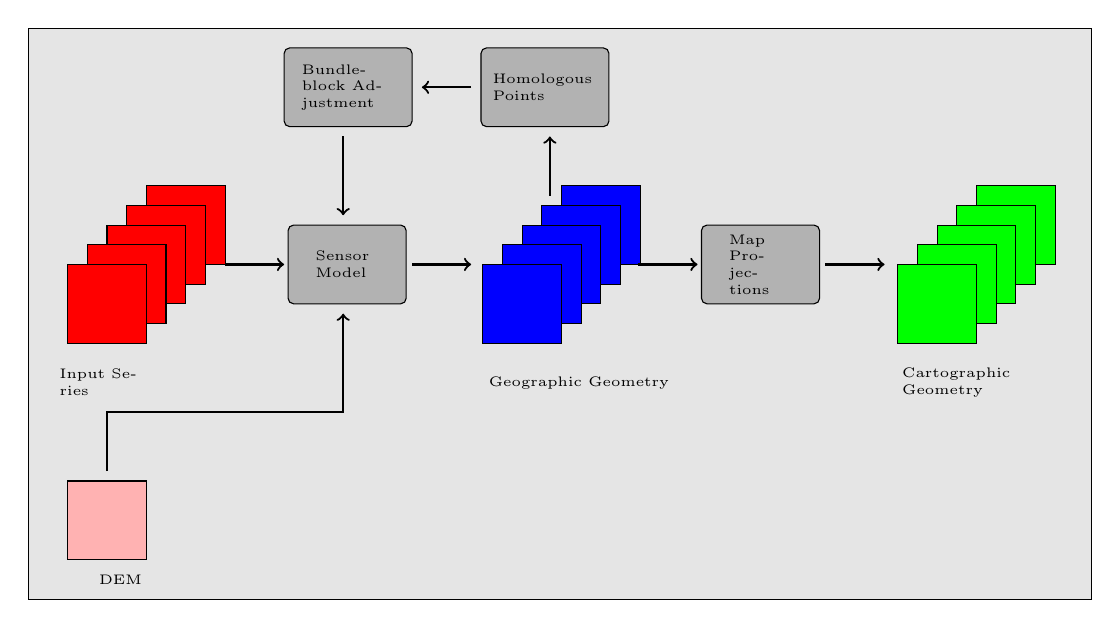
\begin{tikzpicture}[scale=0.25]
    \tiny
    \draw[fill=black!10] (-1,-12) rectangle (53,17);
     \foreach \x in {5,...,1}
       \draw[fill=red] (\x,\x) rectangle +(4,4);
     \node[fill=black!10, text width= 1.2cm] (InputSeries) at
       (3,-1) {Input Series};
     
     \draw[->,thick] (9,5) --  +(3,0);
     
     \draw[fill=black!30,rounded corners=2pt] (12.2,3) rectangle +(6,4);
     \node[text width= 0.7cm] (SensorModel) at (15,5) {Sensor Model};
     
     \draw[fill=red!30] (1,-10) rectangle +(4,4);
     \node[fill=black!10, text width= 1.2cm] (DEM) at
       (5,-11) {DEM};
     
     \draw[->,thick] (3,-5.5) --  ++(0,3) -- ++(12,0) -- ++(0,5);
     
     \draw[->,thick] (18.5,5) --  +(3,0);
     
     \foreach \x in {5,...,1}
       \draw[fill=blue,xshift=600pt] (\x,\x) rectangle +(4,4);
     \node[fill=black!10, text width= 2.8cm] (GeographicGeometry) at
       (28,-1) {Geographic Geometry};

      

       \draw[->,thick] (25.5,8.5) --  +(0,3);
       
     \draw[fill=black!30,rounded corners=2pt] (22,12) rectangle +(6.5,4);
     \node[text width= 0.7cm] (HomPoExtr) at (24,14) {Homologous
     Points};

     \draw[->,thick] (21.5,14) --  +(-2.5,0);

     \draw[fill=black!30,rounded corners=2pt] (12,12) rectangle +(6.5,4);
     \node[text width= 1.3cm] (BBAdj) at (15.5,14) {Bundle-block
     Adjustment};

     \draw[->,thick] (15,11.5) --  +(0,-4);

     
      \draw[->,thick] (30,5) --  +(3,0);
      
     \draw[fill=black!30,rounded corners=2pt] (33.2,3) rectangle +(6,4);
     \node[text width= 0.7cm] (MapProjection) at (36,5) {Map Projections};
     

     
     \draw[->,thick] (39.5,5) --  +(3,0);
     
     \foreach \x in {5,...,1}
       \draw[fill=green,xshift=1200pt] (\x,\x) rectangle +(4,4);
     \node[fill=black!10, text width= 1.8cm] (CartographicGeometry) at
       (47,-1) {Cartographic Geometry};
     
     %\draw[->,thick] (36,2) --  ++(0,-10) -- ++(-30,0);
       
  \end{tikzpicture}
  \itkcaption[Image Ortho-registration Procedure]{Image Ortho-registration Procedure.}
\label{fig:ImageOrtho-registrationProcedure}
\end{figure}

This chapter introduces the functionnalities available in OTB for
image ortho-registration. We define ortho-registration as the
procedure allowing to transform an image in sensor geometry to a
geographic or cartographic projection.\\

Figure \ref{fig:ImageOrtho-registrationProcedure} shows a synoptic
view of the different steps involved in a classical ortho-registration
processing chain able to deal with image series. These steps are the following:
\begin{itemize}
  \item Sensor modelling: the geometric sensor model allows to convert
  image coordinates (line, column) into geographic coordinates
  (latitude, longitude); a rigorous modelling needs a digital
  elevation model (DEM) in order to take into account the terrain
  topography.
  \item Bundle-block adjustment: in the case of image series, the
  geometric models and their parameters can be refined by using
  homologous points between the images. This is an optional step and
  not currently implemented in OTB.
  \item Map projection: this step allows to go from geographic
  coordinates to some specific cartographic projection as Lambert,
  Mercator or UTM.
\end{itemize}


\section{Sensor Models}
\ifitkFullVersion
\label{sec:SensorModels}
\fi

A sensor model is a set of equations giving the relationship between
image pixel $(l,c)$ coordinates and ground $(X,Y)$ coordinates for every
pixel in the image. Typically, the ground coordinates are given in a
geographic projection (latitude, longitude). The sensor model
can be expressed either from image to ground -- forward model -- or
from ground to image -- inverse model. This can be written as follows:

\begin{displaymath}
  \begin{array}{cc}
    Forward & \\
    X = f_x(l,c,h,\vec\theta) & Y = f_y(l,c,h,\vec\theta)\\
     & \\ 
    Inverse & \\
    l = g_l(X,Y,h,\vec\theta) & c = g_c(X,Y,h,\vec\theta)
  \end{array}
\end{displaymath}

Where $\vec\theta$ is the set of parameters which describe the sensor
and the acquisition geometry (platform altitude, viewing angle, focal
length for optical sensors, doppler centroid for SAR images, etc.).\\

In OTB, sensor models are implemented as \doxygen{itk}{Transform}s
(see section \ref{sec:Transforms} for details), which are the
appropiate way to express coordinate changes. The base class for
sensor models is \doxygen{otb}{SensorModelBase} from which the classes
\doxygen{otb}{InverseSensorModel} and
\doxygen{otb}{ForwardSensorModel} inherit.\\

As one may note from the model equations, the height of the ground, $h$,
must be known. Usually, that means that a Digital Elevation Model,
DEM, will be used.\\
  

\subsection{Types of Sensor Models}
\label{sec:TypesofSensorModels}
There exist two main types of sensor models. On one hand, we have the
so-called {\em physical models}, which are rigorous, complex,
eventually highly non-linear equations of the sensor geometry. As
such, they are difficult to inverse (obtain the inverse model from the
forward one and vice-versa). They have the significant advantage of having
parameters with physical meaning (angles, distances, etc.). They are
specific of each sensor, which means that a library of models is
required in the software. A library which has to be updated every time a new
sensor is available.\\

On the other hand, we have general analytical models, which
approximate the physical models. These models can take the form of
polynomials or ratios of polynomials, the so-called rational
polynomial functions or Rational Polynomial Coefficients, RPC, also
known as {\em Rapid Positioning Capability}.
Since they are approximations, they are less accurate than the
physical models. However, the achieved accuracy is usually high: in
the case of Pl\'eiades, RPC models have errors lower than 0.02 pixels
with respect to the physical model. Since these models have a standard
form they are easier to use and implement. However, they have the
drawback of having parameters (coefficients, actually) without
physical meaning.\\

OTB, through the use of the OSSIM library --
\url{http://www.ossim.org} -- offers models for most of current
sensors either through a physical or an analytical approach. This is
transparent for the user, since the geometrical model for a given
image is instantiated using the information stored in its meta-data.\\

\subsection{Using Sensor Models}
\label{sec:UsingSensorModels}

The transformation of an image in sensor geometry to geographic
geometry can be done using the following steps.
  \begin{enumerate}
    \item Read image meta-data and instantiate the model with the
    given parameters.
  \item Define the ROI in ground coordinates (this is your output
  pixel array)
  \item Iterate through the pixels of coordinates $(X,Y)$:
    \begin{enumerate}
      \item Get $h$ from the DEM
      \item Compute $(c,l) = G(X,Y,h,\vec\theta)$
      \item Interpolate pixel values if $(c,l)$ are not grid coordinates.
    \end{enumerate}
  \end{enumerate}

Actually, in OTB, you don't have to manually instantiate the sensor
model which is appropriate to your image. That is, you don't have to
manually choose a SPOT5 or a Quickbird sensor model. This task is
automatically performed by the \doxygen{otb}{ImageFileReader} class in
a similar way as the image format recognition is done. The appropriate
sensor model will then be included in the image meta-data, so you can
access it when needed.

\ifitkFullVersion
\input{SensorModelExample.tex}
\fi



\subsection{Limits of the Approach}
\label{LimitsoftheApproach}

As you may understand by now, accurate geo-referencing needs accurate
DEM and also accurate sensor models and parameters. In the case where
we have several images acquired over the same area by different
sensors or different geometric configurations, geo-referencing (geographical coordinates) or ortho-rectification
(cartographic coordinates) is not usually enough. Indeed, when working
with image series we usually want to compare them (fusion, change
detection, etc.) at the pixel level.\\

Since common DEM and sensor parameters do not allow for such an
accuracy, we have to use clever strategies to improve the
co-registration of the images. The classical one consists in refining
the sensor parameters by taking homologous points between the images
to co-register. This is called bundle block adjustment and will be
implemented in comming versions of OTB.

Even if the model parameters are refined, errors due to DEM accuracy
can not be eliminated. In this case, image to image registration can
be applied. This approaches are presented in chapters
\ref{chap:ImageRegistration} and \ref{sec:DisparityMapEstimation}.

%% \section{Bundle-block adjustment}
%% Problem position
%%   \begin{itemize}
%%     \item The image series is geo-referenced (using the available DEM,
%%     and the prior sensor parameters).
%%     \item We assume that homologous points (GCPs, etc.) can be easily
%%     obtained from the geo-referenced series : $HP_i = (X_i,Y_i,h_i)$
%%     \item For each image, and each point, we can write:
%%     $(l_{ij},c_{ij}) = G_j(X_i,Y_i,h_i,\vec\theta_j)$
%%   \end{itemize}

%% \begin{tikzpicture}[scale=0.15]
%% \draw[fill=yellow!20] (-5.5,-15.5) rectangle (5.5,-5.5);
%%     \draw[step=0.5, gray, very thin] (-5.5,-15.5) grid (5.5,-5.5);

%%     \draw[fill=green!20,rotate=10] (-15.5,0.5) rectangle (-5.5,10.5);
%%     \draw[step=0.5, gray, very thin,rotate=10] (-15.5,0.5) grid>
%%     (-5.5,10.5);

%%     \draw[fill=blue!20,rotate=-10] (5.5,0.5) rectangle (15.5,10.5);
%%     \draw[step=0.5, gray, very thin,rotate=-10] (5.5,0.5) grid
%%     (15.5,10.5);

    
%%     \draw[fill=red!70] (1,-11) circle (0.2);
    
%%     \draw (1,-11) .. controls +(30:1cm) and +(60:1cm) .. (-10,7);
    
%%     \draw[fill=red!70] (-10,7) circle (0.2);
    
%%     \node (eq1) at (-12.2,-4) {$\scriptstyle{G_1(X_i,Y_i,h_i,\vec\theta_1)}$};
    
%%     \draw (1,-11) .. controls +(-30:1cm) and +(-60:1cm) .. (10,7);
    
%%     \draw[fill=red!70] (10,7) circle (0.2);
    
%%     \node (eq2) at (7.2,-3) {$\scriptstyle{G_2(X_i,Y_i,h_i,\vec\theta_2)}$};
    
%% \end{tikzpicture}
%% \begin{itemize}
%%       \item Everything is known.
%% \end{itemize}



%% Model refinement
%%   \begin{itemize}
%%     \item If we define $\vec\theta_j^R = \vec\theta_j +
%%     \vec{\Delta\theta_j}$ as the refined parameters,
%%     $\vec{\Delta\theta_j}$ are the unknowns of the model refinement
%%     problem.
%%     \item We have much more equations than unknowns if enough HPs are
%%     found.
%%     \item We solve using non-linear least squares estimation.
%%       \begin{itemize}
%% 	\item The derivatives of the sensor model with respect to its
%% 	parameters are needed.
%%       \end{itemize}
%%   \end{itemize}
  

%% Homologous point extraction
%% From manual to automatic procedures
%% \begin{itemize}
%%   \item Manual extraction can be used for a few images and for a few
%%   points
%%   \item We are interested in many images (long time series) and many
%%   points (in order to reduce registration errors)
%%   \item Proposed procedure
%%     \begin{enumerate}
%%       \item Choose candidate points
%%       \item Define a similarity measure
%%       \item Optimize the measure
%%     \end{enumerate}
%% \end{itemize}

%% Salient points
%% Similarity measures

  
\section{Map Projections}
\ifitkFullVersion
\label{sec:MapProjections}
\fi

Map projections describe the link between geographic coordinates and
cartographic ones. So map projections allow to represent a 2-dimensional manifold of a
3-dimensional space (the Earth surface) in a 2-dimensional space (a
map which used to be a sheet of paper!). This geometrical
transformation doesn't have a unique solution, so over the cartography
history, every country or region in the world has been able to express
the belief of being the center of the universe. In other words, every
cartographic projection tries to minimize the distortions of the 3D to
2D transformation for a given point of the Earth surface\footnote{We
  proposed to optimize an OTB map projection for Toulouse, but we
  didn't get any help from OTB users.}.

In OTB the \doxygen{otb}{MapProjection} class is derived from the
\doxygen{itk}{Transform} class, so the coordinate transformation
points are overloaded with map projection equations. The
\doxygen{otb}{MapProjection} class is templated over the type of
cartographic projection, which is provided by the OSSIM library. In
order to hide the complexity of the approach, some type definitions
for the more common projections are given in the file
\code{otbMapProjections.h} file.

You will seldom use a map projection by itself, but rather in an
ortho-rectification framework. An example is given in the next section.




\section{Ortho-rectification with OTB}
\ifitkFullVersion
\label{sec:OrthorectificationwithOTB}
\input{OrthoRectificationExample.tex}
\fi

\chapter{ Radiometry }

Remote sensing is not just a matter of taking pictures, but also --
mostly -- a matter of measuring physical values. In order to properly
deal with physical magnitudes, the numerical values provided by the
sensors have to be calibrated. After that, several indices with
physical meaning can be computed.

Calibration functionnalities (absolute and relative) and even
atmospheric correction routines will be available in future versions
of OTB. Please note that the 6S Radiative Transfer Code\footnote{\url{http://6s.ltdri.org/}} is already included in the OTB source code and
compiles out of the box. Calibration and atmospheric corrections in
OTB will be based on it.

In the current version of OTB, several vegetation indices are already
available. They are presented in this chapter.


%%%%%%%%%%%%%%%%%%%%%%%%%%%%%%%%%%%%%%%%%%%%%%%%%%%%%%%%%%%%%%%%%%%%%%
\section{Vegetation Index}
\label{sec:VegetationIndex}

\subsection{Introduction}
A vegetation index is a quantitative measure used to measure biomass
or vegetative vigor, usually formed from combinations of several
spectral bands, whose values are added, divided, or multiplied in
order to yield a single value that indicates the amount or vigor of
vegetation.

\subsection{NDVI}
\label{secNDVI}
NDVI was one of the most successful of many attempts to simply and
quickly identify vegetated areas and their {\em condition}, and it remains
the most well-known and used index to detect live green plant canopies
in multispectral remote sensing data. Once the feasibility to detect
vegetation had been demonstrated, users tended to also use the NDVI to
quantify the photosynthetic capacity of plant canopies. This, however,
can be a rather more complex undertaking if not done properly.
\input{NDVIRAndNIRVegetationIndexImageFilter.tex}

\subsection{ARVI}
\label{secARVI}
\input{ARVIMultiChannelRAndBAndNIRVegetationIndexImageFilter.tex}



\section{Atmospheric Corrections}
\label{secAtmosphericCorrections}
\input{AtmosphericCorrectionSequencement.tex}

\chapter{Image Fusion }\label{sec:Fusion}
%\section{Introduction}

Satellite sensors present an important diversity in terms of characteristics.
Some provide a high spatial resolution while other focus on providing several
spectral bands. The fusion process brings the information from different
sensors with different characteristics together to get the best of both
worlds.

Most of the fusion methods in the remote sensing community deal with
the {\em pansharpening technique}. This fusion combines the image from
the PANchromatic sensor of one satellite (high spatial resolution
data) with the multispectral (XS) data (lower resolution in several
spectral bands) to generate images with a high resolution and several
spectral bands. Several advantages make this situation easier:

\begin{itemize}
\item PAN and XS images are taken simultaneously from the same satellite (or
with a very short delay);
\item the imaged area is common to both scenes;
\item many satellites provide these data (SPOT 1-5, Quickbird, Pleiades)
\end{itemize}

This case is well-studied in the literature and many methods exist. Only very
few are available in OTB now but this should evolve soon.



\section{Bayesian Data Fusion}\label{secBayesian}


\input{BayesianFusionImageFilter.tex}

\chapter{Feature Extraction}
\section{Introduction}
What is feature extraction
\section{Radiometric Features}
\input{TouziEdgeDetectorExample}
\section{Geometric Features}
\subsection{Interest Points}
\input{HarrisExample}
\subsection{Alignments}
\label{sec:Alignments}
\input{AlignmentsExample}
\subsection{Lines}
\subsection{Geometric Moments}

Using the algebraic moment theory, H. Ming-Kuel obtained a family of 7
invariants with respect to planar transformations called Hu invariants,
\cite{hu}. Those invariants can be seen as nonlinear combinations of
complex geometric moments:
\begin {equation}
c_{pq} = \int\limits_{-\infty}^{+\infty}\int\limits_{-\infty}^{+\infty}(x + iy)^p(x- iy)^qf(x,y)dxdy,
\label{2.2}
\end{equation}
where $x$ and $y$ are the coordinates of the image $f(x,y)$, $i$ is the
imaginary unit and
$p+q$ is the order of $c_{pq}$. The geometric moments are
particularly useful in the case of scale changes. Hu invariants have
been very much used in object recognition during the last 30 years,
since they are invariant to rotation, scaling and translation. \cite{flusserinv} gives their expressions :

\begin{equation}
\begin{array}{cccc}
\phi_1 = c_{11};& \phi_2 = c_{20}c_{02};& \phi_3 = c_{30}c_{03};& \phi_4 = c_{21}c_{12};\\
\phi_5 = Re(c_{30}c_{12}^3);& \phi_6 = Re(c_{21}c_{12}^2);& \phi_7 = Im(c_{30}c_{12}^3).&\\
\end{array}
\end{equation}


\cite{dudani} have used these invariants for the recognition of
aircraft silhouettes. Flusser and Suk have used them for image
registration, \cite{flusser_2}. They have been modified and
improved by several authors. Flusser used these moments in order to
produce a new family of descriptors of order higher than 3,
\cite{flusserinv}. These descriptors are invariant to scale and
rotation. They have the following expressions:
\begin {equation}
\begin{array}{ccc}
\psi_1  = c_{11} = \phi_1; &  \psi_2  = c_{21}c_{12} = \phi_4; & \psi_3  = Re(c_{20}c_{12}^2) = \phi_6;\\
\psi_4  = Im(c_{20}c_{12}^2); & \psi_5  = Re(c_{30}c_{12}^3) = \phi_5;
& \psi_6  = Im(c_{30}c_{12}^3) = \phi_7.\\
\psi_7  = c_{22}; & \psi_8  = Re(c_{31}c_{12}^2); & \psi_9  = Im(c_{31}c_{12}~2);\\
\psi_{10} = Re(c_{40}c_{12}^4); & \psi_{11} = Im(c_{40}c_{12}^2). &\\

\end{array}
\end {equation}

OTB allows the computation of complex moments and Flusser and Hu
moments, and those can be computed on images and paths.

\textbf{Mettra a jour quand la classe sera corrigee}
\input{ComplexMomentImageExample}
%% \input{ComplexMomentFunctionExample}

%% \input{FlusserMomentImageExample}
%% \input{FlusserMomentFunctionExample}



\chapter{Multi-scale Analysis}
\section{Introduction}

In this chapter, the tools for multi-scale and multi-resoltuion
processing (analysis, synthesis and fusion) will be presented.


%% \section{Pyramidal Approaches}
%% \subsection{Les algorithmes pyramidaux}\label{sec:pyramidaux}
%% \indent Les analyses pyramidales permettent une décomposition multi-résolution de l'image et étaient à l'origine utilisées en compression. Elles se basent sur le principe suivant : une fois l'image filtrée par un filtre passe-bas, elle ne contient plus de détail dont la fréquence spatiale soit supérieure au seuil du filtrage. Si le filtrage est linéaire, on peut donc, en vertu du théorème de Shannon, sous-échantillonner l'image d'un facteur dépendant du seuil du filtrage, et ce sans perte d'information (nous verrons dans la section \ref{sec:pyr_mor} les précautions à prendre pour l'utilisation de filtres non-linéaires).  L'application d'une décomposition pyramidale s'effectue donc de manière récursive en 3 étapes :

%% \begin{enumerate}
%% \item Application à l'image $I_{n}$ d'un opérateur d'un filtrage de nature passe-bas,
%% \item Extraction des différences $D_{n}$ entre l'image filtrée $F(I_{n})$et l'image $I_{n}$, qui correspondent aux détails extraits au niveau n,
%% \item Sous échantillonage de l'image filtrée $F(I_{n})$, ce qui donnera l'image originale au niveau n+1.
%% \end{enumerate}

%% \indent Le résultat obtenu est une succession d'images contenant les détails de l'image à des résolutions de plus en plus basses, et dont la taille est réduite du facteur de sous-échantillonnage à chaque étape. La dernière image produite contient tous les détails dont la fréquence spatiale est inférieure au seuil du dernier filtrage. La figure \ref{pyr_an} propose un synoptique de la phase d'analyse d'un algorithme pyramidal.\\

%% \indent Une fois la phase d'analyse effectuée, on dispose théoriquement de toute l'information de l'image, codée de manière optimale : en effet chaque détail est représenté à la fréquence d'analyse la plus basse respectant le théorème de Shanon. On peut alors effectuer une reconstruction dans le cadre de la compression d'image, ou pour fusionner deux sources d'informations multi-résolution. Cette reconstruction est théoriquement sans perte, si l'on considère des filtres parfaits et le respect absolu des conditions de Shanon. Cette reconstruction s'effectue également de manière récursive, en deux étapes :
%% \begin{enumerate}
%% \item Sur-échantillonage de l'image $I_{n+1}$ à la résolution de l'image $I_{n}$
%% \item Ajout des détails $D_{n}$ extraits au niveau n, ce qui donnera l'image originale au niveau n.
%% \end{enumerate}

%% \indent La figure \ref{pyr_rec} propose un synoptique de la phase de reconstruction d'un algorithme pyramidal.


%% %% \begin{figure}[!ht]
%% %% \begin{center}
%% %% \includegraphics[width=0.7\textwidth]{pyr_an}
%% %% \end{center}
%% %% \caption{Synoptique de la phase d'analyse d'un algorithme pyramidal}
%% %% \label{pyr_an}
%% %% \end{figure}

%% %% \begin{figure}[!hb]
%% %% \begin{center}
%% %% \includegraphics[width=0.7\textwidth]{pyr_rec}
%% %% \end{center}
%% %% \caption{Synoptique de la phase de reconstruction d'un algorithme pyramidal}
%% %% \label{pyr_rec}
%% %% \end{figure}


\subsection{Morphological pyramid}\label{secMorphoPyr}
Pyramidal decompositions are usually based on the following statement: once an
image has been smoothed with a linear filter, it does not contain
any more high-frequency details. Therefore, it can be down-sampled
without any loss of information, according to Shannon Theorem. By
iterating the same smoothing on the down-sampled image, a
multi-resolution decomposition of the scene is
computed. If the smoothing filter is a morphological filter, this
is no longer true, as the filter is not linear. However, by keeping
the details possibly lost in the down-sampling operation, such a
decomposition can be used. 

The Morphological Pyramid is an approach to such a
decomposition. It's computation process is an iterative analysis
involving smoothing by the morphological filter, computing the
details lost in the smoothing, down-sampling the current image, and
computing the details lost in the down-sampling.

\input{MorphologicalPyramidAnalyseFilterExample.tex}

\input{MorphologicalPyramidSynthesisFilterExample.tex}




\chapter{Image Segmentation}
Segmentation of remote sensing images is a challenging task. A myriad
of different methods have been proposed and implemented in recent
years. In spite of the huge effort invested in this problem, there is
no single approach that can generally solve the problem of
segmentation for the large variety of image modalities existing today.

The most effective segmentation algorithms are obtained by carefully
customizing combinations of components. The parameters of these components are
tuned for the characteristics of the image modality used as input and the
features of the objects to be segmented. 

The Insight Toolkit provides a basic set of algorithms that can be used to
develop and customize a full segmentation application. They are
therefore available in the Orfeo Toolbox. Some of the most
commonly used segmentation components are described in the following
sections.


\section{Region Growing}

Region growing algorithms have proven to be an effective approach for image
segmentation. The basic approach of a region growing algorithm is to start
from a seed region (typically one or more pixels) that are considered to be
inside the object to be segmented. The pixels neighboring this region are
evaluated to determine if they should also be considered part of the
object. If so, they are added to the region and the process continues as long
as new pixels are added to the region.  Region growing algorithms vary
depending on the criteria used to decide whether a pixel should be included
in the region or not, the type connectivity used to determine neighbors, and
the strategy used to visit neighboring pixels.

Several implementations of region growing are available in ITK.  This section
describes some of the most commonly used.

\subsection{Connected Threshold}

A simple criterion for including pixels in a growing region is to evaluate
intensity value inside a specific interval.

\label{sec:ConnectedThreshold}
\input{ConnectedThresholdImageFilter.tex}

\subsection{Otsu Segmentation}
Another criterion for classifying pixels is to minimize the error of misclassification.
The goal is to find a threshold that classifies the image into two clusters such that 
we minimize the area under the histogram for one cluster that lies on the other cluster's 
side of the threshold. This is equivalent to minimizing the within class variance
or equivalently maximizing the between class variance.

\label{sec:OtsuThreshold}
\ifitkFullVersion 
\input{OtsuThresholdImageFilter.tex}
\fi

\label{sec:OtsuMultipleThreshold}
\ifitkFullVersion 
\input{OtsuMultipleThresholdImageFilter.tex}
\fi

\subsection{Neighborhood Connected}
\label{sec:NeighborhoodConnectedImageFilter}
\ifitkFullVersion 
\input{NeighborhoodConnectedImageFilter.tex}
\fi


\subsection{Confidence Connected}
\label{sec:ConfidenceConnected}
\ifitkFullVersion 
%\input{ConfidenceConnected.tex}
%\input{ConfidenceConnectedOnBrainWeb.tex}
\fi




\subsection{Isolated Connected}
\label{sec:IsolatedConnected}
\ifitkFullVersion 
%\input{IsolatedConnectedImageFilter.tex}
\fi


\subsection{Confidence Connected in Vector Images}
\label{sec:VectorConfidenceConnected}
\ifitkFullVersion 
%\input{VectorConfidenceConnected.tex}
\fi


\section{Segmentation Based on Watersheds}
\label{sec:WatershedSegmentation}
\ifitkFullVersion 
%\input WatershedSegmentation.tex
\fi


% the clearpage command helps to avoid orphans in the title of the next
% section.
\clearpage

\section{Level Set Segmentation}
\label{sec:LevelSetsSegmentation}
\ifitkFullVersion 
%%%%%%%%%%%%%%%%%%%%%%%%%%%%%%%%%%%%%%%%%%%%%%%%%%%%%%%%%%%%%%%%%%%%%%%%%
%
%
%     This file is included from the file   Segmentation.tex
% 
%     Section tag and label are placed in this top file.
%
%
%
%%%%%%%%%%%%%%%%%%%%%%%%%%%%%%%%%%%%%%%%%%%%%%%%%%%%%%%%%%%%%%%%%%%%%%%%



\itkpiccaption[Zero Set Concept]{Concept of zero set in a level set.\label{fig:LevelSetZeroSet}}
\parpic(9cm,6cm)[r]{\includegraphics[width=8cm]{LevelSetZeroSet.eps}}

The paradigm of the level set is that it is a numerical method for tracking
the evolution of contours and surfaces. Instead of manipulating the contour
directly, the contour is embedded as the zero level set of a higher
dimensional function called the level-set function, $\psi(\bf{X},t)$. The
level-set function is then evolved under the control of a differential
equation.  At any time, the evolving contour can be obtained by extracting
the zero level-set $\Gamma(\bf(X),t) =
\{\psi(\bf{X},t) = 0\}$ from the output.  The main advantages of using level
sets is that arbitrarily complex shapes can be modeled and topological
changes such as merging and splitting are handled implicitly. 

Level sets can be used for image segmentation by using image-based features
such as mean intensity, gradient and edges in the governing differential
equation.  In a typical approach, a contour is initialized by a user and is
then evolved until it fits the form of an object in the image.
Many different implementations and variants of this basic concept have been
published in the literature. An overview of the field has been made by
Sethian \cite{Sethian1996}.

The following sections introduce practical examples of some
of the level set segmentation methods available in ITK.  The remainder of this
section describes features common to all of these filters except the
\doxygen{itk}{FastMarchingImageFilter}, which is derived from a different code
framework.  Understanding these features will aid in using the filters
more effectively.

Each filter makes use of a generic level-set equation to compute the update to
the solution $\psi$ of the partial differential equation.

\begin{equation}
\label{eqn:LevelSetEquation}
\frac{d}{dt}\psi = -\alpha \mathbf{A}(\mathbf{x})\cdot\nabla\psi - \beta
  P(\mathbf{x})\mid\nabla\psi\mid + 
\gamma Z(\mathbf{x})\kappa\mid\nabla\psi\mid
\end{equation}
 
where $\mathbf{A}$ is an advection term, $P$ is a propagation (expansion) term,
and $Z$ is a spatial modifier term for the mean curvature $\kappa$.  The scalar
constants $\alpha$, $\beta$, and $\gamma$ weight the relative influence of
each of the terms on the movement of the interface.  A segmentation filter may
use all of these terms in its calculations, or it may omit one or more terms.
If a term is left out of the equation, then setting the corresponding scalar
constant weighting will have no effect.

All of the level-set based segmentation filters \emph{must} operate with
floating point precision to produce valid results.  The third, optional
template parameter is the \emph{numerical type} used for calculations and as
the output image pixel type.  The numerical type is \code{float} by default,
but can be changed to \code{double} for extra precision.  A user-defined,
signed floating point type that defines all of the necessary arithmetic
operators and has sufficient precision is also a valid choice.  You should
not use types such as \code{int} or \code{unsigned char} for the numerical
parameter.  If the input image pixel types do not match the numerical type,
those inputs will be cast to an image of appropriate type when the filter is
executed.

Most filters require two images as input, an initial model $\psi(\bf{X},
t=0)$, and a \emph{feature image}, which is either the image you wish to
segment or some preprocessed version.  You must specify the isovalue that
represents the surface $\Gamma$ in your initial model. The single image
output of each filter is the function $\psi$ at the final time step.  It is
important to note that the contour representing the surface $\Gamma$ is the
zero level-set of the output image, and not the isovalue you specified for
the initial model.  To represent $\Gamma$ using the original isovalue, simply
add that value back to the output.

The solution $\Gamma$ is calculated to subpixel precision.  The best discrete
approximation of the surface is therefore the set of grid positions closest to
the zero-crossings in the image, as shown in
Figure~\ref{fig:LevelSetSegmentationFigure1}.  The
\doxygen{itk}{ZeroCrossingImageFilter} operates by finding exactly those grid 
positions and can be used to extract the surface. 


\begin{figure}
\centering
\includegraphics[width=0.4\textwidth]{LevelSetSegmentationFigure1.eps}
\itkcaption[Grid position of the embedded level-set surface.]{The implicit level
set surface $\Gamma$ is the black line superimposed over the image grid.  The location
of the surface is interpolated by the image pixel values.  The grid pixels
closest to the implicit surface are shown in gray. }
\protect\label{fig:LevelSetSegmentationFigure1}
\end{figure}

There are two important considerations when analyzing the processing time for
any particular level-set segmentation task: the surface area of the evolving
interface and the total distance that the surface must travel.  Because the
level-set equations are usually solved only at pixels near the surface (fast
marching methods are an exception), the time taken at each iteration depends on
the number of points on the surface.  This means that as the surface grows, the
solver will slow down proportionally.  Because the surface must evolve slowly
to prevent numerical instabilities in the solution, the distance the surface
must travel in the image dictates the total number of iterations required.

Some level-set techniques are relatively insensitive to initial conditions
and are therefore suitable for region-growing segmentation. Other techniques,
such as the \doxygen{itk}{LaplacianSegmentationLevelSetImageFilter}, can easily
become ``stuck'' on image features close to their initialization and should
be used only when a reasonable prior segmentation is available as the
initialization.  For best efficiency, your initial model of the surface
should be the best guess possible for the solution. 


\subsection{Fast Marching Segmentation}
\label{sec:FastMarchingImageFilter}

\ifitkFullVersion
\input{FastMarchingImageFilter.tex}
\fi


%% \subsection{Shape Detection Segmentation}
%% \label{sec:ShapeDetectionLevelSetFilter}

%% \ifitkFullVersion
%% \input{ShapeDetectionLevelSetFilter.tex}
%% \fi


%% \subsection{Geodesic Active Contours Segmentation}
%% \label{sec:GeodesicActiveContourImageFilter}

%% \ifitkFullVersion
%% \input{GeodesicActiveContourImageFilter.tex}
%% \fi


%% \subsection{Threshold Level Set Segmentation}
%% \label{sec:ThresholdSegmentationLevelSetImageFilter}
%% \ifitkFullVersion
%% \input{ThresholdSegmentationLevelSetImageFilter.tex}
%% \fi


%% \subsection{Canny-Edge Level Set Segmentation}
%% \label{sec:CannySegmentationLevelSetImageFilter}
%% \ifitkFullVersion
%% \input{CannySegmentationLevelSetImageFilter.tex}
%% \fi


%% \subsection{Laplacian Level Set Segmentation}
%% \label{sec:LaplacianSegmentationLevelSetImageFilter}
%% \ifitkFullVersion
%% \input{LaplacianSegmentationLevelSetImageFilter.tex}
%% \fi

%% \subsection{Geodesic Active Contours Segmentation With Shape Guidance}
%% \label{sec:GeodesicActiveContourShapePriorLevelSetImageFilter}
%% \ifitkFullVersion
%% \input{GeodesicActiveContourShapePriorLevelSetImageFilter.tex}
%% \fi



\fi


\section{Hybrid Methods} 
\label{sec:HybridSegmentationMethods}

\ifitkFullVersion 
%%%%%%%%%%%%%%%%%%%%%%%%%%%%%%%%%%%%%%%%%%%%%%%%%%%%%%%%%%%%%%%%%%%%%%%%%
%
%
%     This file is included from the file   Segmentation.tex
% 
%     Section tag and label are placed in this top file.
%
%
%
%%%%%%%%%%%%%%%%%%%%%%%%%%%%%%%%%%%%%%%%%%%%%%%%%%%%%%%%%%%%%%%%%%%%%%%%

\subsection{Introduction}
\label{sec:HybridSegmentationIntroduction}
This section introduces the use of hybrid methods for segmentation of image
data. The hybrid segmentation approach integrates boundary-based and
region-based segmentation methods that amplify the strength but reduce the
weakness of both techniques. The advantage of this approach comes from
combining region-based segmentation methods like the fuzzy connectedness and
Voronoi diagram classification with boundary-based deformable model
segmentation. The synergy between fundamentally different methodologies tends
to result in robustness and higher segmentation quality.  A hybrid
segmentation engine can be built, as illustrated in
Figure~\ref{fig:ComponentsofaHybridSegmentationApproach}. It consists of
modules representing segmentation methods and implemented as ITK filters. We
can derive a variety of hybrid segmentation methods by exchanging the filter
used in each module. It should be noted that under the fuzzy connectedness
and deformable models modules, there are several different filters that can
be used as components. Below, we describe two examples of hybrid segmentation
methods, derived from the hybrid segmentation engine: integration of fuzzy
connectedness and Voronoi diagram classification (hybrid method 1), and
integration of Gibbs prior and deformable models (hybrid method 2).  Details
regarding the concepts behind these methods have been discussed in the
literature
\cite{Angelini2002,Udupa2002,Jin2002,Imielinska2001,Imielinska2000a,Imielinska2000b}


\subsection{Fuzzy Connectedness and Confidence Connectedness }

Probably the simplest combination of hybrid filters is the pair formed by the
\doxygen{ConfidenceConnectednessImageFilter} and
\doxygen{SimpleFuzzyConnectednessScalarImageFilter}. In this combination the
confidence connectedness filter is used to produce a rough segmentation of an
object and to compute and estimation of the mean and variance of
gray values in such structure. The values of mean and variance are then passed
to the Simple Fuzzy Connectedness image filter in order to compute an affinity map.

\ifitkFullVersion
\input{FuzzyConnectednessImageFilter.tex}
\fi



\subsection{Fuzzy Connectedness and Voronoi Classification}
\label{sec:HybridMethod1}
In this section we present a hybrid segmentation method that requires
minimal manual initialization by integrating the fuzzy connectedness and
Voronoi diagram classification segmentation algorithms. We start with a fuzzy
connectedness filter to generate a sample of tissue from a region to be
segmented. From the sample, we automatically derive image statistics that
constitute the homogeneity operator to be used in the next stage of the
method. The output of the fuzzy connectedness filter is used as a prior to
the Voronoi diagram classification filter. This filter performs iterative
subdivision and classification of the segmented image resulting in an
estimation of the boundary. The output of this filter is a 3D binary image
that can be used to display the 3D result of the segmentation, or passed to
another filter (e.g. deformable model) for further improvement of the final
segmentation. Details describing the concepts behind these methods have been
published in
\cite{Angelini2002,Udupa2002,Jin2002,Imielinska2001,Imielinska2000a,Imielinska2000b}

In Figure~\ref{fig:UMLClassDiagramoftherFuzzyConnectednessFilter}, we
describe the base class for simple fuzzy connectedness segmentation. This
method is non-scale based and non-iterative, and requires only one seed to
initialize it. We define affinity between two nearby elements in a image
(e.g. pixels, voxels) via a degree of adjacency, similarity in their
intensity values, and their similarity to the estimated object.  The closer
the elements and the more similar their intensities, the greater the affinity
between them. We compute the strength of a path and fuzzy connectedness
between each two pixels (voxels) in the segmented image from the fuzzy
affinity.  Computation of the fuzzy connectedness value of each pixel (voxel)
is implemented by selecting a seed point and using dynamic programming. The
result constitutes the fuzzy map. Thresholding of the fuzzy map gives a
segmented object that is strongly connected to the seed point (for more
details, see \cite{Udupa1996}). Two fuzzy connectedness filters are available
in the toolkit:

\begin{itemize}
\item The \doxygen{SimpleFuzzyConnectednessScalarImageFilter}, an implementation of the
fuzzy connectedness segmentation of single-channel (grayscale) image.
\item The \doxygen{SimpleFuzzyConnectednessRGBImageFilter}, an implementation
of fuzzy connectedness segmentation of a three-channel (RGB) image.
\end{itemize}

New classes can be derived from the base class by defining other affinity
functions and targeting multi-channel images with an arbitrary number of
channels. Note that the simple fuzzy connectedness filter can be used as a
stand-alone segmentation method and does not necessarily need to be combined
with other methods as indicated by
Figure~\ref{fig:UMLCollaborationDiagramoftheFuzzyConnectednessFilter}.

In Figure~\ref{fig:UMLVoronoiSegmentationClassFilter} we present the base
class for Voronoi diagram classification. We initialize the method with a
number of random seed points and compute the Voronoi diagram over the
segmented 2D image. Each Voronoi region in the subdivision is classified as
internal or external, based on the homogeneity operator derived from the
fuzzy connectedness algorithm.  We define boundary regions as the external
regions that are adjacent to the internal regions.  We further subdivide the
boundary regions by adding seed points to them. We converge to the final
segmentation using simple stopping criteria (for details, see
\cite{Imielinska2001}). Two Voronoi-based segmentation methods are available in ITK: the \doxygen{VoronoiSegmentationImageFilter} for processing single-channel
(grayscale) images, and the \doxygen{VoronoiSegmentationRGBImageFilter}, for
segmenting three-channel (RGB) images. New classes can be derived from the
base class by defining other homogeneity measurements and targeting
multichannel images with an arbitrary number of channels.  The other classes
that are used for computing a 2D Voronoi diagram are shown in
Figure~\ref{fig:UMLClassesforImplementationofVoronoiDiagramFilter}. Note that
the Voronoi diagram filter can be used as a stand-alone segmentation method,
as depicted in
Figure~\ref{fig:UMLCollaborationDiagramoftheVoronoiSegmentationFilter}.

Figures~\ref{fig:UMLHybridMethodDiagram1} and 
\ref{fig:UMLHybridMethodDiagram2} illustrate hybrid segmentation methods
that integrate fuzzy connectedness with Voronoi diagrams, and fuzzy
connectedness, Voronoi diagrams and deformable models, respectively.


\begin{figure}
\center
\includegraphics[width=0.8\textwidth]{HybridSegmentationEngine1.eps}
\itkcaption[Hybrid Segmentation Engine]{The hybrid segmentation engine.}
\label{fig:ComponentsofaHybridSegmentationApproach}
\end{figure}


\begin{figure}
\center
\includegraphics[width=0.8\textwidth]{FuzzyConnectednessClassDiagram1.eps}
\itkcaption[FuzzyConectedness Filter Diagram]{Inheritance diagram for the fuzzy connectedness filter.}
\label{fig:UMLClassDiagramoftherFuzzyConnectednessFilter}
\end{figure}


\begin{figure}
\center
\includegraphics[width=0.8\textwidth]{FuzzyConnectednessCollaborationDiagram1.eps}
\itkcaption[Fuzzy Connectedness Segmentation Diagram]{Inputs and outputs to
FuzzyConnectednessImageFilter segmentation algorithm.}
\label{fig:UMLCollaborationDiagramoftheFuzzyConnectednessFilter}
\end{figure}

\begin{figure}
\center
\includegraphics[width=0.8\textwidth]{VoronoiSegmentationClassDiagram1.eps}
\itkcaption[Voronoi Filter class diagram]{Inheritance diagram for the Voronoi
segmentation filters.}
\label{fig:UMLVoronoiSegmentationClassFilter}
\end{figure}

\begin{figure}
\center
\includegraphics[width=0.8\textwidth]{VoronoiSegmentationCollaborationDiagram1.eps}
\itkcaption[Voronoi Diagram Filter classes]{Classes used by the Voronoi 
segmentation filters.}
\label{fig:UMLClassesforImplementationofVoronoiDiagramFilter}
\end{figure}


\begin{figure}
\center
\includegraphics[width=0.8\textwidth]{VoronoiSegmentationCollaborationDiagram2.eps}
\itkcaption[Voronoi Diagram Segmentation]{Input and output to the 
VoronoiSegmentationImageFilter.}
\label{fig:UMLCollaborationDiagramoftheVoronoiSegmentationFilter}
\end{figure}


\begin{figure}
\center
\includegraphics[width=0.8\textwidth]{FuzzyVoronoiCollaborationDiagram1.eps}
\itkcaption[Fuzzy Connectedness and Voronoi Diagram Classification]{Integration
 of the fuzzy connectedness and Voronoi segmentation filters.}
\label{fig:UMLHybridMethodDiagram1}
\end{figure}

\begin{figure}
\center
\includegraphics[width=0.8\textwidth]{FuzzyVoronoiDeformableCollaborationDiagram1.eps}
\itkcaption[Fuzzy Connectedness, Voronoi diagram, and Deformable
Models]{Integration of the fuzzy connectedness, Voronoi, and 
deformable model segmentation methods.}
\label{fig:UMLHybridMethodDiagram2}
\end{figure}



\subsubsection{Example of a Hybrid Segmentation Method}
\label{sec:HybridMethod1:Example}

%\ifitkFullVersion
%\input{HybridSegmentationFuzzyVoronoi.tex}
%\fi




%% \subsection{Deformable Models and Gibbs Prior}

%% Another combination that can be used in a hybrid segmentation method is the
%% set of Gibbs prior filters with deformable models.

%% \subsubsection{Deformable Model}
%% \ifitkFullVersion
%% \input{DeformableModel1.tex}
%% \fi


%% \subsubsection{Gibbs Prior Image Filter}
%% \ifitkFullVersion
%% \input{GibbsPriorImageFilter1.tex}
%% \fi


\fi


\section{Feature Extraction} 
\label{sec:FeatureExtractionMethods}

\ifitkFullVersion 
%\input{FeatureExtractionMethods.tex}
\fi



\chapter{Image Simulation}

This chapter deals with image simulation algorithm. Using objects transmittance and reflectance and sensor characteristics, it can be possible to generate realistic hyperspectral synthetic set of data. This chapter includes PROSPECT (leaf optical properties) and SAIL (canopy bidirectional reflectance) model. Vegetation optical properties are modeled using PROSPECT model \cite{Jacquemoud2009}. 

\section{PROSAIL model}

PROSAIL \cite{Jacquemoud2009} model is the combinaison of PROSPECT leaf optical properties model and SAIL canopy bidirectional reflectance model. PROSAIL has also been used to develop new methods for retrieval of vegetation biophysical properties. It links the spectral variation of canopy reflectance, which is mainly related to leaf biochemical contents, with its directional variation, which is primarily related to canopy architecture and soil/vegetation contrast. This link is key to simultaneous estimation of canopy biophysical/structural variables for applications in agriculture, plant physiology, or ecology, at different scales. PROSAIL has become one of the most popular radiative transfer tools due to its ease of use, general robustness, and consistent validation by lab/field/space experiments over the years. Here we present a first example, which returns Hemispheric and Viewing reflectance for wavelength sampled  from $400$ to $2500 nm$. Inputs are leaf and Sensor (intrinsic and extrinsic) characteristics. 

\label{sec:Prosail}
\input{ProsailModel.tex}


\section{Image Simulation}

Here we present a complete pipeline to simulate image using sensor characteristics and objects reflectance and transmittance properties. This example use :

\begin{itemize}
\item input image
\item label image : describes image object properties.
\item label properties : describes each label characteristics.
\item mask : vegetation image mask.
\item cloud mask (optionnal).
\item acquisition rarameter file : file containing the parameters for the acquisition.
\item RSR File : File name for the relative spectral response to be used.
\item sensor FTM file : File name for sensor spatial interpolation.
\end{itemize}

Algorithm is divided in following step :

\begin{enumerate}
\item LAI (Leaf Area Index) image estimation using NDVI formula.
\item Sensor Reduce Spectral Response (RSR) using PROSAIL reflectance output interpolated at sensor spectral bands.
\item Simulated image using Sensor RSR and Sensor FTM.
\end{enumerate}

\subsection{LAI image estimation}

\label{sec:LAIFromNDVI}
\input{LAIFromNDVIImageTransform.tex}

\subsection{Sensor RSR Image Simulation}

\label{sec:LAIAndPROSAILToSensorResponse}
\input{LAIAndPROSAILToSensorResponse.tex}

% the clearpage command helps to avoid orphans in the title of the next
% section.
\clearpage



\chapter{Dimension Reduction}\label{chap:dimred}

Dimension reduction is a statistical process which concentrates the
amount of information in multivariate data into a fewer number of
variables (or dimensions).

Though there are plenty of non-linear methods in the litterature, OTB
provides only linear dimension reduction techniques applied to images for now.

Usually, linear dimension-reduction algorithms try to find a set of
linear combinations of the input image bands that maximise a given
criterion, often chosen so that image information concentrates on the
first components. Algorithms differs by the criterion to optimise and
also by their handling of the signal or image noise.

In remote-sensing images processing, dimension reduction algorithms
are of great interest for denoising, or as a preliminary processing
for classification of feature images or unmixing of hyperspectral
images. In addition to the denoising effect, the advantage of
dimension reduction in the two latter is that it lowers the size of
the data to be analysed, and as such, speeds up the processing time
without too much loss of accuracy.

\section{Principal Component Analysis}

\input{PCAExample}

\section{Noise-Adjusted Principal Components Analysis}

\input{NAPCAExample}

\section{Maximum Noise Fraction}

\input{MNFExample}

\section{Fast Independant Component Analysis}

\input{ICAExample}

\section{Maximum Autocorrelation Factor}

\input{MaximumAutocorrelationFactor}



\chapter{Classification}

\section{Introduction}

In statistical classification, each object is represented by $d$ features (a
measurement vector), and the goal of classification becomes finding compact and
disjoint regions (decision regions\cite{Duda2000}) for classes in a
$d$-dimensional feature space. Such decision regions are defined by decision
rules that are known or can be trained.  The simplest configuration of a
classification consists of a decision rule and multiple membership functions;
each membership function represents a class. Figure~\ref{fig:simple}
illustrates this general framework.

\begin{figure}[h]
  \centering
  \includegraphics[width=0.7\textwidth]{DudaClassifier.eps}
  \itkcaption[Simple conceptual classifier]{Simple conceptual classifier.}
  \label{fig:simple}
\end{figure}

This framework closely follows that of Duda and
Hart\cite{Duda2000}. The classification process can be described
as follows:

\begin{enumerate}
\item{A measurement vector is input to each membership function.}
\item{Membership functions feed the membership scores to the
    decision rule.}
\item{A decision rule compares the membership scores and returns a
    class label.}
\end{enumerate}

\begin{figure}
  \centering
  \includegraphics[width=0.7\textwidth]{StatisticalClassificationFramework.eps}
  \itkcaption[Statistical classification framework]{Statistical classification
framework.}
  \protect\label{fig:StatisticalClassificationFramework}
\end{figure}

This simple configuration can be used to formulated various classification
tasks by using different membership functions and incorporating task specific
requirements and prior knowledge into the decision rule. For example, instead
of using probability density functions as membership functions, through
distance functions and a minimum value decision rule (which assigns a class
from the distance function that returns the smallest value) users can achieve a
least squared error classifier. As another example, users can add a rejection
scheme to the decision rule so that even in a situation where the membership
scores suggest a ``winner'', a measurement vector can be flagged as ill
defined. Such a rejection scheme can avoid risks of assigning a class label
without a proper win margin.

Note that to use these concepts into your own programs, you might have to link
to other OTB libraries (edit the \code{TARGET\_LINK\_LIBRARIES} to add them),
for example OTBLearning, OTBMarkov.

\section{Unsupervised classification}

\subsection{K-Means Classification}
\label{sec:KMeansClassifier}

\subsubsection{Simple version}
\ifitkFullVersion
\input{ScalarImageKmeansClassifier.tex}
\fi
\ifitkFullVersion
\input{ScalarImageKmeansModelEstimator.tex}
\fi

\subsubsection{General approach}
\ifitkFullVersion
\input{KMeansImageClassificationExample.tex}
\fi

\subsubsection{k-d Tree Based k-Means Clustering}
\label{sec:KdTreeBasedKMeansClustering}
\ifitkFullVersion
\input{KdTreeBasedKMeansClustering.tex}
\fi

\subsection{Kohonen's Self Organizing Map}
\label{sec:SOM}
The Self Organizing Map, SOM, introduced by Kohonen is a
non-supervised neural
learning algorithm. The map is composed of neighboring cells which are
in competition by means of mutual interactions and they adapt in order
to match characteristic patterns of the examples given during the
learning. The SOM is usually on a plane (2D).

The algorithm implements a nonlinear projection from a high
dimensional feature space to a lower dimension space, usually 2D. It
is able to find the correspondence between a set of structured data
and a network of much lower dimension while keeping the topological
relationships existing in the feature space. Thanks to this
topological organization, the final map presents clusters and their
relationships. 

%\subsection{The algorithm}
Kohonen's SOM is usually represented as an array of cells where each
cell is, $i$, associated to a feature (or weight) vector  $\underline m_i = \left[m_{i1},m_{i2},\cdots,m_{in}\right]^T\in
\mathbb{R}^n$ (figure \ref{carte}).\\
\begin{figure}
\center
\includegraphics[width=0.45\textwidth]{carte.eps}
\itkcaption[Kohonen's Self Organizing Map]{Kohonen's Self Organizing Map}
\label{carte}
\end{figure}

A cell (or neuron) in the map is a good detector for a given input
vector $\underline x = \left[x_{1},x_{2},\cdots,x_{n}\right]^T\in
\mathbb{R}^n$ if the latter is {\em close} to the former. This
distance between vectors can be represented by the scalar product 
$\underline{x}^T\cdot\underline{m_i}$, but for most of the cases other
distances can be used, as for instance the Euclidean one. The cell
having the weight vector closest to the input vector is called the
{\em winner}.

%\subsubsection{Learning}
The goal of the learning step is to get a map which is representative
of an input example set. It is an iterative procedure which consists
in passing each input example to the map, testing the response of each
neuron and modifying the map to get it closer to the examples.

\begin{algo}
SOM learning:
\begin{enumerate}
\item $t=0$.
\item Initialize the weight vectors of the map (randomly, for instance).
\item While $t<$ number of iterations, do:
\begin{enumerate}
\item $k=0$.
\item While $k<$ number of examples, do:
\begin{enumerate}
\item Find the vector $\underline{m}_i(t)$ which minimizes the distance
$d(\underline{x}_k,\underline{m}_i(t))$
\item For a neighborhood $N_c(t)$ around the winner cell, apply the transformation:
\begin{equation}
\underline{m}_i(t+1)=\underline{m}_i(t)+\beta(t)\left[\underline{x}_k(t)-\underline{m}_i(t)\right]
\label{khoupdate}
\end{equation}
\item $k=k+1$
\end{enumerate}
\item $t=t+1$.
\end{enumerate}

\end{enumerate}
\end{algo}


In \ref{khoupdate}, $\beta(t)$ is a decreasing function with the
geometrical distance to the winner cell. For instance:
\begin{equation}
\beta(t)=\beta_0(t)e^{-\frac{\parallel \underline{r}_i -  \underline{r}_c\parallel^2}{\sigma^2(t)}},
\end{equation}
with $\beta_0(t)$ and $\sigma(t)$ decreasing functions with time and
$\underline{r}$ the cell coordinates in the output -- map -- space.\\

Therefore the algorithm consists in getting the map closer to the
learning set. The use of a neighborhood around the winner cell allows
the organization of the map into areas which specialize in the
recognition of different patterns. This neighborhood also ensures that
cells which are topologically close are also close in terms of the
distance defined in the feature space.


%%%1. Construction SOM
\subsubsection{Building a color table}
\label{sec:SOMColorTable}
\input{SOMExample}
\subsubsection{SOM Classification}
\label{sec:SOMClassification}
\input{SOMClassifierExample}

\subsubsection{Multi-band, streamed classification}

\ifitkFullVersion
\input{SOMImageClassificationExample.tex}
\fi

%%%2. Lecture SOM et ensemble de vecteurs autre image pour construire
%%%ActivationMAP 

%\subsection{Bayesian classification}

\subsection{Bayesian Plug-In Classifier}
\label{sec:BayesianPluginClassifier}

\ifitkFullVersion 
\input{BayesianPluginClassifier.tex}
\fi


\subsection{Expectation Maximization Mixture Model Estimation}
\label{sec:ExpectationMaximizationMixtureModelEstimation}

\ifitkFullVersion 
\input{ExpectationMaximizationMixtureModelEstimator.tex}
\fi




%%%%%%%%%%%%%%%%%%%%%%%%%%%%%%%%%%%%%%%%%%%%%%%%%%%%%%%%%%%%%%%%%%%%%%
\subsection{Statistical Segmentations}
\label{sec:StatisticalSegmentations}

%\subsection{Markov Random Fields}

\subsubsection{Stochastic Expectation Maximization}
\label{sec:SEM}

The Stochastic Expectation Maximization (SEM) approach is a stochastic 
version of the EM mixture estimation seen on
section~\ref{sec:ExpectationMaximizationMixtureModelEstimation}. It has been 
introduced by \cite{CeDi95} to prevent convergence of the EM approach from
local minima. It avoids the analytical maximization issued by integrating a
stochastic sampling procedure in the estimation process. It induces an almost
sure (a.s.) convergence to the algorithm.

From the initial two step formulation of the EM mixture estimation, the SEM
may be decomposed into 3 steps:
\begin{enumerate}
\item \textbf{E-step}, calculates the expected membership values for each 
measurement vector to each classes.
\item \textbf{S-step}, performs a stochastic sampling of the membership vector
to each classes, according to the membership values computed in the E-step.
\item \textbf{M-step}, updates the parameters of the membership probabilities
(parameters to be defined through the class
\subdoxygen{itk}{Statistics}{ModelComponentBase} and its inherited classes).
\end{enumerate}
The implementation of the SEM has been turned to a contextual SEM in the sense
where the evaluation of the membership parameters is conditioned to
membership values of the spatial neighborhood of each pixels.

\ifitkFullVersion 
\input{SEMModelEstimatorExample.tex}
\fi


%%%%%%%%%%%%%%%%%%%%%%%%%%%%%%%%%%%%%%%%%%%%%%%%%%%%%%%%%%%%%%%%%%%%%%

\subsection{Classification using Markov Random Fields}
\label{sec:MarkovRandomField}

Markov Random Fields are probabilistic models that use the statistical
dependency between
pixels in a neighborhood to infeer the value of a give pixel.

\subsubsection{ITK framework}
\label{sec:MarkovRandomFieldITK}
The
\subdoxygen{itk}{Statistics}{MRFImageFilter} uses the maximum a posteriori (MAP)
estimates for modeling the MRF. The object traverses the data set and uses the
model generated by the Mahalanobis distance classifier to get the the distance
between each pixel in the data set to a set of known classes, updates the
distances by evaluating the influence of its neighboring pixels (based on a MRF
model) and finally, classifies each pixel to the class which has the minimum
distance to that pixel (taking the neighborhood influence under consideration).
The energy function minimization is done using the iterated conditional modes
(ICM) algorithm \cite{Besag1986}.

\ifitkFullVersion
\input{ScalarImageMarkovRandomField1.tex}
\fi 

\subsubsection{OTB framework}
\label{sec:MarkovRandomFieldOTB}
The ITK approach was considered not to be flexible enough for some
remote sensing applications. Therefore, we decided to implement our
own framework.
\index{Markov}

\begin{figure}[th]
  \centering
  \includegraphics[width=0.7\textwidth]{MarkovFramework.eps}
  \itkcaption[OTB Markov Framework]{OTB Markov Framework.}
  \label{fig:markovFramework}
\end{figure}

\index{Markov!Classification}
\ifitkFullVersion
\input{MarkovClassification1Example.tex}
\fi 

\index{Markov!Classification}
\ifitkFullVersion
\input{MarkovClassification2Example.tex}
\fi 

\index{Markov!Classification}
\ifitkFullVersion
\input{MarkovClassification3Example.tex}
\fi 

\index{Markov!Regularization}
\ifitkFullVersion
\input{MarkovRegularizationExample.tex}
\fi 

\section{Supervised classification}

\subsection{Learning from samples}
\input{TrainMachineLearningModelFromSamplesExample.tex}
%\subsection{Learning from images}
%todo



\section{Support Vector Machines}
\label{sec:SupportVectorMachines}

Kernel based learning methods in general and the Support Vector
Machines (SVM) in particular, have been introduced in the last years
in learning theory for classification and regression tasks,
\cite{vapnik}. SVM have been successfully applied to text
categorization, \cite{joachims}, and face recognition,
\cite{osuna}. Recently, they have been successfully used for the
classification of hyperspectral remote-sensing images, \cite{bruzzoneSVM}.

Simply stated, the approach consists in searching for the separating
surface between 2 classes by the determination of the subset of
training samples which best describes the boundary between the 2
classes. These samples are called support vectors and completely
define the classification system. In the case where the two classes are
nonlinearly separable, the method uses a kernel expansion in order to make
projections of the feature space onto higher dimensionality spaces
where the separation of the classes becomes linear.

 \subsection{Mathematical formulation}

 This section reminds the basic principles of SVM learning and
 classification. A good tutorial on SVM can be found in, \cite{burges}.
 
We have $N$ samples represented by the couple $(y_i,\mathbf{x}_i),
i=1\ldots N$ where $y_i \in \{-1,+1\}$ is the class label and
$\mathbf{x}_i \in \mathbb{R}^n$ is the feature vector of dimension
$n$. A classifier is a function  $$f(\mathbf{x},\boldsymbol{\alpha}) :
\mathbf{x}\mapsto y$$ where $\boldsymbol{\alpha}$ are the classifier
parameters. The SVM finds the optimal separating hyperplane which
fulfills the following constraints :
    \begin{itemize}
      \item The samples with labels $+1$ and $-1$ are on different
      sides of the hyperplane.
      \item The distance of the closest vectors to the hyperplane is
      maximised. These are the support vectors (SV) and this distance is
      called the margin.
    \end{itemize}

    The separating hyperplane has the equation
    $$\mathbf{w}\cdot\mathbf{x}+b=0;$$ with $\mathbf{w}$ being its
    normal vector and $x$ being any point of the hyperplane. The
    orthogonal distance to the origin is given by
    $\frac{|b|}{\|\mathbf{w}\|}$. Vectors located outside the
    hyperplane have either $\mathbf{w}\cdot\mathbf{x}+b>0$ or
      $\mathbf{w}\cdot\mathbf{x}+b<0$.

    Therefore, the classifier function can be written as
    $$f(\mathbf{x},\mathbf{w}, b)=sgn(\mathbf{w}\cdot\mathbf{x}+b).$$
    
The SVs are placed on two hyperplanes which are parallel to the
      optimal separating one. In order to find the optimal
      hyperplane, one sets $\mathbf{w}$ and
      $b$ : $$\mathbf{w}\cdot\mathbf{x}+b=\pm 1.$$

Since there must not be any vector inside the margin, the following
constraint can be used:
    $$\mathbf{w}\cdot\mathbf{x}_i+b\ge +1\text{ if }y_i=+1;$$
    $$\mathbf{w}\cdot\mathbf{x}_i+b\le -1\text{ if }y_i=-1;$$ which
    can be rewritten as $$y_i(\mathbf{w}\cdot\mathbf{x}_i+b)-1\ge 0~  ~ \forall i.$$

    The orthogonal distances of the 2 parallel hyperplanes to the
    origin are $\frac{|1-b|}{\|\mathbf{w}\|}$ and
      $\frac{|-1-b|}{\|\mathbf{w}\|}$. Therefore the modulus of the
    margin is equal to $\frac{2}{\|\mathbf{w}\|}$ and it has to be
    maximised.

    Thus, the problem to be solved is:

	\begin{itemize}
	\item Find $\mathbf{w}$ and $b$ which minimise
	 $\left\{ \frac{1}{2}\|\mathbf{w}\|^2 \right\}$
	\item under the constraint :
	 $y_i(\mathbf{w}\cdot\mathbf{x}_i+b)\ge 1~  ~ i=1\ldots N.$
	\end{itemize}

	This problem can be solved by using the Lagrange multipliers
	with one multiplier per sample. It can be shown that only the
	support vectors will have a positive Lagrange multiplier.

	In the case where the two classes are not exactly linearly
	separable, one can modify the constraints above by using 
      $$\mathbf{w}\cdot\mathbf{x}_i+b\ge +1 - \xi_i \text{ if }y_i=+1;$$
    $$\mathbf{w}\cdot\mathbf{x}_i+b\le -1+\xi_i \text{ if }y_i=-1;$$
    $$\xi_i\ge 0~  ~\forall i.$$

	If $\xi_i > 1$, one considers that the sample is wrong. The
	function which has then to be minimised is
	$\frac{1}{2}\|\mathbf{w}\|^2 + C\left( \sum_i \xi_i\right); $,
	where $C$ is a tolerance parameter. The optimisation problem
	is the same than in the linear case, but one multiplier has to
	be added for each new constraint $\xi_i\ge 0$.

	If the decision surface needs to be non-linear, this solution
	cannot be applied and the kernel approach has to be adopted.


One drawback of the SVM is that, in their basic version, they can only
solve two-class problems. Some works exist in the field of multi-class
SVM (see \cite{allwein00reducing,weston98multiclass}, and the
comparison made by \cite{hsu01comparison}), but they are
not used in our system.

You have to be aware that to achieve better convergence of the algorithm it is 
strongly advised to normalize feature vector components in the $[-1;1]$ 
interval.

For problems with $N > 2$ classes, one can choose either to train $N$
SVM (one class against all the others), or to train $N\times(N-1)$ SVM
(one class against each of the others). In the second approach, which
is the one that we use, the final decision is taken by choosing the
class which is most often selected by the whole set of SVM.


\subsection{Learning With PointSets}
\label{sec:LearningWithPointSets}
\input{SVMPointSetModelEstimatorExample}
\subsection{PointSet Classification}
\label{sec:PointSetClassification}
\input{SVMPointSetClassificationExample}
\subsection{Learning With Images}
\label{sec:LearningWithImages}
\input{SVMImageModelEstimatorExample}
\subsection{Image Classification}
\label{sec:ImageClassification}
\input{SVMImageClassificationExample}
\input{SVMImageEstimatorClassificationMultiExample}
\subsection{Generic Kernel SVM}

OTB has developed a specific interface for user-defined kernels. A function
$k(\cdot,\cdot)$ is considered to be a kernel when:
\begin{align}\label{eqMercer}
        \forall g(\cdot) \in {\cal L}^2(\mathbbm{R}^n) \quad & \text{so 
that} \quad
        \int g(\boldsymbol{x})^2 d\boldsymbol{x} \text{ be finite,} \\
        & \text{then} \quad \int k(\boldsymbol{x},\boldsymbol{y}) \, 
g(\boldsymbol{x})
        \, g(\boldsymbol{y}) \, d\boldsymbol{x} d\boldsymbol{y} \geqslant 0,
        \notag
\end{align}
which is known as the {\em Mercer condition\/}.

When defined through the OTB, a kernel is a class that inherits from
\code{GenericKernelFunctorBase}. Several virtual functions have to 
be overloaded:
\begin{itemize}
\item The \code{Evaluate} function, which implements the behavior of the 
kernel
itself. For instance, the classical linear kernel could be re-implemented
with:
\begin{verbatim}
        double
        MyOwnNewKernel
        ::Evaluate ( const svm_node * x, const svm_node * y,
                     const svm_parameter & param ) const
        {
                return this->dot(x,y);
        }
\end{verbatim}
This simple example shows that the classical dot product is already 
implemented
into \subdoxygen{otb}{GenericKernelFunctorBase}{dot()} as a protected
function.
\item The \code{Update()} function which synchronizes local variables and 
their
integration into the initial SVM procedure. The following examples will show
the way to use it.
\end{itemize}

Some pre-defined generic kernels have already been implemented in OTB:
\begin{itemize}
\item \doxygen{otb}{MixturePolyRBFKernelFunctor} which implements a 
linear mixture
of a polynomial and a RBF kernel;
\item \doxygen{otb}{NonGaussianRBFKernelFunctor} which implements a non
gaussian RBF kernel;
\item \doxygen{otb}{SpectralAngleKernelFunctor}, a kernel that integrates
the Spectral Angle, instead of the Euclidean distance, into an inverse 
multiquadric kernel.
This kernel may be appropriated when using multispectral data.
\item \doxygen{otb}{ChangeProfileKernelFunctor}, a kernel which is
dedicated to the supervized classification of the multiscale change profile
presented in section \ref{sec:KullbackLeiblerProfile}.
\end{itemize}

\subsubsection{Learning with User Defined Kernels}
\label{sec:Learningwithuserdefinedkernel}
\ifitkFullVersion
\input{SVMGenericKernelImageModelEstimatorExample.tex}
\fi

\subsubsection{Classification with user defined kernel}

\ifitkFullVersion
\input{SVMGenericKernelImageClassificationExample.tex}
\fi

\subsection{Multi-band, streamed classification}

\ifitkFullVersion
\input{SVMImageClassifierExample.tex}
\fi

\subsection{Classification map regularization}

\ifitkFullVersion
\input{ClassificationMapRegularizationExample.tex}
\fi





\chapter{Object-based Image Analysis }\label{sec:OBIA}

Object-Based Image Analysis (OBIA) consists in analysing images at
the object level instead of working at the pixel level. This approach
is particularly well adapted for high resolution images and allows
more robust and less noisy results.

OTB allows to implement OBIA by using ITK's Label Object framework
(\url{http://www.insight-journal.org/browse/publication/176}). This
allows to represent a segmented image as a set of regions and not
anymore as a set of pixels. Added to the compression rate achieved by
this kind of description, the main advantage of this approach is the
possibility to operate at the segment (or object level).

A classical OBIA pipeline will use the following steps:

\begin{enumerate}
\item Image segmentation (the whole or only parts of it).
\item Image to LabelObjectMap (a kind of \code{std::map<LabelObject>}) transformation.
\item Eventual relabeling.
\item Attribute computation for the regions using the image before
  segmentation:
  \begin{enumerate}
         \item Shape attributes.
         \item Statistics attributes.
         \item Attributes for radiometry, textures, etc.
  \end{enumerate}

\item Object filtering
  \begin{enumerate}
         \item Remove/select objects under a condition (area less than
         X, NDVI higher than X, etc.)
	 \item Keep N objects.
	 \item etc.
  \end{enumerate}
\item LabelObjectMap to image transformation.
\end{enumerate}


\section{From Images to Objects}\label{sec:FromImagesToObjects}
\input{ImageToLabelToImage.tex}

\section{Object Attributes}\label{sec:ObjectAttributes}
\input{ShapeAttributeComputation.tex}


\section{Object Filtering}
\input{KeepNObjects.tex}

\section{Object-based classification}

\chapter{Change Detection}
\section{Introduction}
Change detection techniques try to detect and locate areas which have
changed between two or more observations of the same scene. These
changes can be of different types, with different origins and of
different temporal length. This allows to distinguish different kinds
of applications:
\begin{itemize}
\item \emph{land use monitoring}, which corresponds to the
  characterization of the evolution of the vegetation, or its seasonal
  changes;
\item \emph{natural resources management}, which corresponds mainly
  to the characterisation of the evolution of the urban areas, the
  evolution of the deforestation, etc.
\item \emph{damage mapping}, which corresponds to the location of
  damages caused by natural or industrial disasters.
\end{itemize}

From the point of view of the observed phenomena, one can distinguish
2 types of changes whose nature is rather different: the abrupt
changes and the progressive changes, which can eventually be
periodic. From the data point of view, one can have:

       \begin{itemize}
       \item Image pairs before and after the event. The applications
       are mainly the abrupt changes.

	 \item Multi-temporal image series on which 2 types on changes
	 may appear:
	 \begin{itemize}
	   \item The slow changes like for instance the erosion,
	   vegetation evolution, etc. The knowledge of the studied
	   phenomena and of their consequences on the geometrical
	   and radiometrical evolution at the different dates is a
	   very important information for this kind of analysis.

	     \item The abrupt changes may pose different kinds of
	     problems depending on whether the date of the change is
	     known in the image series or not. The detection of areas
	     affected by a change occurred at a known date may exploit
	     this a priori information in order to split the image
	     series into two sub-series (before an after) and use the
	     temporal redundancy in order to improve the detection
	     results. On the other hand, when the date of the change
	     is not known, the problem has a higher difficulty.

	 \end{itemize}
	 
       \end{itemize}

From this classification of the different types of problems, one can
infer 4 cases for which one can look for algorithms as a function of
the available data:
\begin{enumerate}
\item Abrupt changes in an image pair. This is no doubt the field for
  which more work has been done. One can find tools at the 3 classical
  levels of image processing: data level (differences, ratios, with
  or without pre-filtering, etc.), feature level (edges, targets,
  etc.), and interpretation level (post-classification comparison).

\item Abrupt changes within an image series and a known date. One can
  rely on bi-date techniques, either by fusing the images into 2 stacks
  (before and after), or by fusing the results obtained by different
  image couples (one after and one before the event). One can also use
  specific discontinuity detection techniques to be applied in the
  temporal axis.

\item Abrupt changes within an image series and an unknown date. This
  case can be seen either as a generalization of the preceding one (testing
  the N-1 positions for N dates) or as a particular case of the
  following one.

\item Progressive changes within an image series. One can work in two
  steps:
  \begin{enumerate}
    \item detect the change areas using stability criteria in the
    temporal areas;
    \item identify the changes using prior information about the type
    of changes of interest.
  \end{enumerate}
  
\end{enumerate}




\subsection{Surface-based approaches}\label{secChgtAbr}
In this section we discuss about the damage assessment techniques
which can be applied when only two images (before/after) are available.\\

As it has been shown in recent review works
\cite{Coppin03,Lu04,Radke05,Richards05}, a relatively high number of
methods exist, but most of them have been developed for optical and
infrared sensors. Only a few recent works on change detection with
radar images exist
\cite{Stabel02,Bruzzone02b,Onana_2003,Inglada03,Derrode03,Bazi05,Inglada07}.
However, the intrinsic limits of passive sensors, mainly related to
their dependence on meteorological and illumination conditions, impose
severe constraints for operational applications. The principal
difficulties related to change detection are of four types:

\begin{enumerate}
\item In the case of radar images, the speckle noise makes the image
  exploitation difficult.
\item The geometric configuration of the image acquisition can produce
  images which are difficult to compare.
\item Also, the temporal gap between the two acquisitions an thus the
  sensor aging and the inter-calibration are sources of variability
  which are difficult to deal with.
\item Finally, the normal evolution of the observed scenes must not be
  confused with the changes of interest.
\end{enumerate}

The problem of detecting abrupt changes between a pair of images is
the following: Let $I_{1},I_{2}$ be two images acquired at different
dates $t_{1},t_{2}$; we aim at producing a thematic map which shows
the areas where changes have taken place.

Three main categories of methods exist:

\begin{itemize}
\item{Strategy $1$: Post Classification Comparison}

The principle of this approach \cite{Deer_1998} is two obtain two
land-use maps independently for each date and comparing them. 



\item{Strategy $2$: Joint classification}

This method consists in producing the change map directly from a joint
classification of both images.

\item{Strategy $3$: Simple detectors}

The last approach consists in producing an image of change likelihood
(by differences, ratios or any other approach) and thresholding it in
order to produce the change map.

\end{itemize}


Because of its simplicity and its low computation overhead, the third
strategy is the one which has been chosen for the CNES processing
chain presented in this document.



\section{Change Detection Framework}
\label{sec:ChangeDetectionFramework}
\input{ChangeDetectionFrameworkExample.tex}
\section{Simple Detectors}
\label{sec:SimpleDetectors}
\subsection{Mean Difference}
\label{sec:MeanDifference}

The simplest change detector is based on the pixel-wise differencing
of image values: 
\begin{equation}
I_{D}(i,j)=I_{2}(i,j)-I_{1}(i,j).
\end{equation}

In order to make the algorithm robust to noise, one actually uses
local means instead of pixel values.

\input{DiffChDet}

\subsection{Ratio Of Means}
\label{sec:RatioOfMeans}

This detector is similar to the previous one except that it uses a
ratio instead of the difference:
\begin{equation}
\displaystyle I_{R}(i,j) = \frac{\displaystyle I_{2}(i,j)}{\displaystyle I_{1}(i,j)}.
\end{equation}

The use of the ratio makes this detector robust to multiplicative
noise which is a good model for the speckle phenomenon which is
present in radar images.

In order to have a bounded and normalized detector the following
expression is actually used:


\begin{equation}
\displaystyle I_{R}(i,j) = 1 - min \left(\frac{\displaystyle I_{2}(i,j)}{\displaystyle I_{1}(i,j)},\frac{\displaystyle I_{1}(i,j)}{\displaystyle I_{2}(i,j)}\right).
\end{equation}


\input{RatioChDet}


\section{Statistical Detectors}
\label{sec:StatisticalDetectors}

\subsection{Distance between local distributions}
\label{sec:KullbackLeiblerDistance}

This detector is similar to the ratio of means detector (seen in the 
previous section page~\pageref{sec:RatioOfMeans}). Nevertheless, 
instead of the comparison of means, the comparison is performed to
the complete distribution of the two Random Variables (RVs)~\cite{Inglada03}.

The detector is based on the Kullback-Leibler distance between probability 
density functions (pdfs). In the neighborhood of each pixel of the pair 
of images $I_1$ and $I_2$ to be compared, the distance between local pdfs 
$f_1$ and $f_2$ of RVs $X_1$ and $X_2$ is evaluated by:
\begin{align}
  {\cal K}(X_1,X_2) &= K(X_1|X_2) + K(X_2|X_1) \\
  \text{with} \qquad
  K(X_j | X_i) &= \int_{\mathbbm{R}} 
      \log \frac{f_{X_i}(x)}{f_{X_j}(x)} f_{X_i}(x) dx,\qquad i,j=1,2.
\end{align}
In order to reduce the computational time, the local pdfs $f_1$ and $f_2$ 
are not estimated through histogram computations but rather by a cumulant
expansion, namely the Edgeworth expansion, with is based on the 
cumulants of the RVs:
\begin{equation}\label{eqEdgeworthExpansion}
f_X(x) = \left( 1 + \frac{\kappa_{X;3}}{6} H_3(x) 
					+ \frac{\kappa_{X;4}}{24} H_4(x)
					+ \frac{\kappa_{X;5}}{120} H_5(x)
					+ \frac{\kappa_{X;6}+10 \kappa_{X;3}^2}{720} H_6(x) \right) {\cal G}_X(x).
\end{equation}
In eq.~\eqref{eqEdgeworthExpansion}, ${\cal G}_X$ stands for the Gaussian pdf
which has the same mean and variance as the RV $X$. The $\kappa_{X;k}$
coefficients are the cumulants of order $k$, and $H_k(x)$ are the 
Chebyshev-Hermite polynomials of order $k$ (see~\cite{Inglada07} for deeper
explanations).

\input{KullbackLeiblerDistanceChDet}

\subsection{Local Correlation}
\label{sec:LocalCorrelation}
The correlation coefficient measures the likelihood of a linear
relationship between two random variables:
\begin{equation}
\begin{split}
I_\rho(i,j) &= \frac{1}{N}\frac{\sum_{i,j}(I_1(i,j)-m_{I_1})(I_2(i,j)-m_{I_2})}{\sigma_{I_1}
\sigma_{I_2}}\\
& = \sum_{(I_1(i,j),I_2(i,j))}\frac{(I_1(i,j)-m_{I_1})(I_2(i,j)-m_{I_2})}{\sigma_{I_1}
\sigma_{I_2}}p_{ij}
\end{split}
\end{equation}

where $I_1(i,j)$ and $I_2(i,j)$ are the pixel values of the 2 images and
$p_{ij}$ is the joint probability density. This is like using a linear model:
\begin{equation}
I_2(i,j) = (I_1(i,j)-m_{I_1})\frac{\sigma_{I_2}}{\sigma_{I_1}}+m_{I_2}
\end{equation}
for which we evaluate the likelihood with  $p_{ij}$.

With respect to the difference detector, this one will be robust to
illumination changes.
\input{CorrelChDet.tex}

%% \subsection{Mutual Information}

%% Other sophisticated change detectors can be used by applying some
%% concepts of information theory. We have chosen to implement several
%% detectors based on the mutual information measure
%% \cite{Thevenaz2000,Inglada_2002}. This kind of measure needs for the
%% estimation of the joint density probabilities for the pair of images
%% to be compared. Depending on how this estimation is made, one can
%% choose between robust but slow detectors or quick but less robust ones.\\

%% The mutual information is a divergence (some kind of distance) between
%% the joint probability $p_{1,2}$ and the product of marginal ones
%% $p_1\cdot p_2$. Therefore, it is a measure of statistical dependence
%% between the two images and can thus be understood as a generalization
%% of the correlation coefficient. This means that it can be applied to
%% the multi-sensor case.\\

%% The divergence used is written as:
%% \begin{equation}
%% K(P,Q) = \int p \log\frac{p}{q},
%% \end{equation}

%% so the mutual information detector is written as:


%% \begin{equation}
%% I_{MI}(i,j) = \int p_{1,2} \log\frac{p_{1,2}}{p_1\cdot p_2}.
%% \end{equation}


%% \subsubsection{Joint histogram}
%% In this version of the detector, a joint probability density $p_{ij}$ is
%% estimated only once for the pair of images. This makes it a rather
%% quick detector.
%% \subsubsection{Local histogram}
%% This version uses a local estimation of the probabilities in the
%% neighborhood of each pixel. It is the slowest detector, but the most
%% robust one.
%% \subsubsection{Cumulant-based}

%% This version is the quickest one, but it is only an approximation of the
%%     mutual information. Indeed, a probability density can be
%%     reconstructed from a series expansion of its cumulants. The
%%     cumulants are defined as follows:
%% \begin{subequations}
%% \begin{equation}
%% E\left[\prod_{k \in N} X_k\right]=\sum_{N_1\cup\cdot\cdot\cdot \cup
%% N_n=N}cum(X_k, k \in N_1)\cdot\cdot\cdot cum(X_k,k\in N_n)=\kappa_k,
%% \end{equation}
%% \begin{equation}
%% cum(X_k, k\in N)=\sum_{N_1\cup\cdot\cdot\cdot \cup N_n=N}
%% (-1)^{n-1}(n-1)!E\left[\prod_{k\in N_1} X_k \right]\cdot\cdot\cdot
%% E\left[\prod_{k\in N_n} X_k \right],
%% \end{equation}
%% \end{subequations}

%% For instance, one has 
        
%% \begin{equation}
%% cum(X_1,X_2)=E(X_1,X_2)-(EX_1)(EX_2)=cov(X_1,X_2).
%% \end{equation}

%% \begin{equation}
%%   \begin{split}
%%     cum(X_1,X_2,X_3)=&E(X_1,X_2,X_3)-E(X_1,X_2)(EX_3)-E(X_1,X_3)(EX_2)\\
%%     & -E(X_2,X_3)(EX_1)+2(EX_1)(EX_2)(EX_3)
%%   \end{split}
%% \end{equation}

%% Using these cumulants, the series expansion of the probability density
%% function $f(x)$ can be written as a modulation of the normalized
%% Gaussian function $\Phi(x)$:


%%       \begin{equation}
%%   f(x) \approx  \Phi(x)\left[ P_0(x) +
%%   P_1(x)\frac{1}{\sqrt{n}}+ P_2(x)\frac{1}{n} + ...+ P_r(x)\frac{1}{n^{r/2}}\right],
%% \end{equation}
%% with
%% \begin{subequations}
%%   \begin{equation}
%%     P_0(x) = 1,
%%   \end{equation}
%%   \begin{equation}
%%     P_1(x) = \frac{\kappa_3}{3!}H_3(x),
%%   \end{equation}
%%   \begin{equation}
%%     P_2(x) = \frac{\kappa_4}{4!}H_4(x) + \frac{10\kappa_3^2}{6!}H_6(x),
%%   \end{equation}
%% \end{subequations}
%% and the Hermite polynomials
%% \begin{subequations}
%%   \begin{equation}
%%     H_0(x) = 1,
%%   \end{equation}
%%   \begin{equation}
%%     H_1(x) = x,
%%   \end{equation}
%%   \begin{equation}
%%     H_2(x) = x^2 -1,
%%   \end{equation}
%%   \begin{equation}
%%     H_3(x) = x^3-3x.
%%   \end{equation}
%% \end{subequations}

%% When thiese approximations are used in the expression of the mutual
%% information, one has the following result:
    
%%     \begin{equation}
%% I_{IM}(i,j)({\underline Y})\approx \frac{1}{4}\sum_{kl\neq
%% kk}\left(cum_2(Y_k,Y_l)\right)^2+\frac{1}{48}\sum_{klmn\neq
%% kkkk}\left(cum_4(Y_k,Y_l,Y_m,Y_n)\right)^2,
%% \label{kim}
%% \end{equation}
%%  where $\{k,l,m,n\}$ can take the values 1 and 2 (the image index) and
%%  the cumulants are computed in the neighborhood if the pixel of
%%  coordinates $(i,j)$.


\section{Multi-Scale Detectors}
\label{sec:MultiScaleDetectors}

\subsection{Kullback-Leibler Distance between distributions}
\label{sec:KullbackLeiblerProfile}

This technique is an extension of the distance between distributions 
change detector presented in section~\ref{sec:KullbackLeiblerDistance}.
Since this kind of detector is based on cumulants estimations through
a sliding window, the idea is just to upgrade the estimation of the cumulants
by considering new samples as soon as the sliding window is increasing in size.

Let's consider the following problem: how to update the moments when a
$N+1^{th}$ observation $x_{N+1}$ is added to a set of observations $\{x_1, x_2, \ldots,
x_N\}$ already considered.
The evolution of the central moments may be characterized by:
\begin{align}\label{eqMomentN}
	\mu_{1,[N]} & = \frac{1}{N} s_{1,[N]} \\
	\mu_{r,[N]} & = \frac{1}{N} \sum_{\ell = 0}^r \binom{r}{\ell} 
									\left( -\mu_{1,[N]} \right)^{r-\ell}
									s_{\ell,[N]}, \notag
\end{align}
where the
notation $s_{r,[N]} = \sum_{i=1}^N x_i^r$ has been used.
Then, Edgeworth series is updated also by transforming moments to
cumulants by using:
\begin{equation}\label{eqCumsMoms}
  \begin{split}
\kappa_{X;1} &= \mu_{X;1}\\
\kappa_{X;2} &= \mu_{X;2}-\mu_{X;1}^2\\
\kappa_{X;3} &= \mu_{X;3} - 3\mu_{X;2} \mu_{X;1} + 2\mu_{X;1}^3\\
\kappa_{X;4} &= \mu_{X;4} - 4\mu_{X;3} \mu_{X;1} - 3\mu_{X;2}^2 + 12 \mu_{X;2} \mu_{X;1}^2 - 6\mu_{X;1}^4.
  \end{split}
\end{equation}
It yields a set of images that represent the change measure according to an
increasing size of the analysis window.

\input{KullbackLeiblerProfileChDet}






\chapter{Hyperspectral}

%TODO translate 
Une image hyperspectrale de la Terre acquises depuis
un porteur aérien ou spatial contient une collection de pixels
spectraux ou, de manière équivalente, une collection de bandes
spectrales.

\begin{figure}[h]
  \centering
  \includegraphics[width=0.7\textwidth]{Cube_HPX.eps}
  \itkcaption[Hyperspectral cube]{Illustration d'un cube hyperspectral, d'un pixel spectral et
d'une bande spectrale.}
  \label{fig:cube}
\end{figure}

Le cube hyperspectral \ref{fig:cube} acquis est une image de
radiance, chaque pixel spectral contient une information spectrale
fine qui dépend : 

\begin{enumerate}
\item{Du spectre de la source lumineuse (en pratique, le
soleil) et des perturbations atmosphériques.}
\item{Des réponses spectrales
des différents matériaux présents dans la zone de recouvrement et de la nature de leur mélange.}
\end{enumerate}

Des traitements préliminaires de
correction atmosphérique permettent d'estimer un cube de réflectance
spectrale par soustraction de l'information extrinsèque à la
scène. 

\section{Unmixing}

L'information de réflectance ne dépend que des spectres de
réflectance des matériaux de la scène. Lorsque le mélange entre les
matériaux est macroscopique, le modèle de mélange linéaire de spectres
est généralement admis. La scène imagée a typiquement l'allure
illustrée ci-après :

\begin{figure}[h]
  \centering
  \includegraphics[width=0.7\textwidth]{Linear_Unmixing_HPX.eps}
  \itkcaption[Modele de melange linear]{ Schéma d'une zone vérifiant le modèle MML.}
  \label{fig:linear_unmixing}
\end{figure}

Nous notons \ref{fig:linear_unmixing}  la
présence de pixels-purs et de pixels-mélanges. Le MML admet que le
spectre de réflectance associé à chaque pixel est une combinaison
linéaire des spectres de matériaux purs composant la zone de
recouvrement, communément appelés ``endmembers''. Cela peut être
illustré \ref{fig:decomp_mml} :

\begin{figure}[h]
  \centering
  \includegraphics[width=0.7\textwidth]{Decomposition_MML_HPX.eps}
  \itkcaption[Decomposition Modele de melange linear]{Décomposition d'un cube hyperspectral selon le MML.}
  \label{fig:decomp_mml}
\end{figure}

Le ``terme'' de gauche représente les différentes bandes spectrales du
cube de données. Le ``terme'' de droite représente un ``produit''
entre les spectres de réflectance des endmembers et leurs cartes
d'abondances respectives. La carte d'abondance d'un endmembers est une
image en niveaux de gris compris entre $0$ et $1$. Le pixel i de la carte
d'abondance du endmember j a pour valeur $s_{ji}$. Cette valeur est
l'abondance du endmember j dans le pixel i. Sous certaines conditions
[Huck2009], cette valeur peut être interprétée comme le ratio
surfacique du matériau dans la zone de recouvrement (\ref{fig:linear_unmixing}).  En
pratique, on peut raisonnablement s'attendre: 

\begin{enumerate}
\item{à ce qu'un nombre
limité de matériaux purs composent la scène.}
\item{à ce que la scène
contienne des pixels purs si la résolution spatiale est suffisante, et
n'en contienne pas forcément sinon.}
\end{enumerate}
 
De nombreuses techniques d'analyse d'images hyperspectrales reposent
sur une approche géométrique ou chaque pixel spectral est vu comme un
vecteur de dimension L (nombre de bandes spectrales). Les
bandes spectrales peuvent alors être écrites sous forme vectorisée.

%% Figure 5: "Vectorisation" du cube hyperspectral. Les pixels spectraux
%% sont rangés dans les colonnes de la matrice R et, de manière
%% équivalente, les bandes spectrales sont rangées dans les lignes de R.

Par déduction de \ref{fig:decomp_mml} et de la Figure5, le MML consiste à décomposer R
de la manière suivante : $R= A.S + N = X + N$

Soit J le nombre de endmembers et I le nombre de pixels spectaux: 
\begin{enumerate}
\item{Les J colonnes de la matrice A contiennent les spectres de endmembers.}
\item{Les J lignes de la matrice S contiennent les cartes d'abondances
vectorisées;nous appelons vecteurs d'abondances les colonnes de la
matrice S.}
\item{La matrice N, de dimensions $LxI$, est une matrice de bruit
additif.}
\end{enumerate}

   

Le problème du démixage consiste à estimer les matrices A et S à
partir de R ou éventuellement de Xchapeau, une estimation de la matrice signal
débruité.

Remarque: Plusieurs contraintes physiques peuvent être prises en
compte pour permettre la résolution de ce problème: 
C1: positivité
des spectres de réflectance (matrice A non-négative); 
C2: positivité
des abondances (matrice S non-négative); 
C3: additivité des
abondances (la somme des coefficients de chaque colonne de la matrice
S vaut 1); 
L'indépendance algébrique entre les ``vecteurs spectraux''
associés au endmembers et la linéarité des mélanges de spectres, d'ou
découle la propriété du simplexe décrite au paragraphe suivant.
Simplexe circonscrit aux données Les algorithmes récents de démixage
s'appuient sur la ``propriété du simplexe''. Dans un espace vectoriel
de dimension $J-1$, on peut associer à J vecteurs algébriquement
indépendants J points définissant les sommets d'un J-simplexe, comme
l'illustre la Figure 6.

Figure 6: Illustration d'un 2-simplexe, d'un 3-simplexe et d'un
4-simplexe.  Un cube hyperspectral de L bandes, basé sur J endmembers,
peut être confiné dans un sous-espace-affine de dimension $J-1$.  Un
sous espace pertinent, au sens du rapport signal-a-bruit, est
généralement obtenu par Analyse en Composantes Principales (ACP). En
pratique, les $J-1$ vecteurs propres associés au plus fortes valeurs
propres forment les colonnes d'une matrice de projection V de
dimension $(Lx(J-1))$. Les données réduites Z, de dimensions $((J-1)xI)$,
sont obtenues par l'opération:

ou chaque colonne de'est vue soustraire le spectre moyen,
généralement estimé au sens du maximum de vraisemblance. Dans le
sous-espace porteur des vecteurs-colonnes de Z, les spectres de
endmembers sont donc associés au sommet d'un simplexe. Si le bruit est
négligeable, ce simplexe circonscrit les données réduites.

Remarque: Cette propriété met en évidence le fait que les endmembers
recherchés sont les sommets d'un simplexe qui circonscrit les
données. Cependant, une infinité de simplexes différents peuvent
circonscrire un même jeu de données. En fait, le problème du démixage
n'a généralement pas de solution unique. Cette dégénérescence peut
aussi être mise en évidence par le formalisme de la factorisation en
matrices non-négatives (voir Huck2010a), qui sera abordé un peu plus
loin. Il convient donc de choisir la solution physiquement la plus
pertinente. Toutes les techniques de démixage basées sur cette
propriété du simplexe admettent que la solution la plus pertinente est
définie par le simplexe admissible de volume minimal, ou la notion de
volume est généralisée à toutes les dimensions finies (éventuellement
différentes de 3).  Sélection d'algorithmes et état de l'art Les
algorithmes de démixage linéaire les plus récents exploitent
généralement la propriété du simplexe. Il est possible de les classer
en plusieurs familles: 
Famille 1 Une première famille d'algorithmes
de démixage est basée sur la recherche des endmembers ``parmi'' les
données. Cela signifie qu'un pixel pur au minimum doit etre associé à
chaque endmembers. Si cette hypothèse n'est pas vérifiée, cela
produira une erreur d'estimation sur les spectres de
endmembers. L'avantage historique de ces algorithmes est leur faible
complexité algorithmique. Les trois plus connus sont PPI (Pixel Purity
Index), NFINDER et VCA (Vertex Component Analysis)
[Nascimento2005]. Outre son succès reconnu par la communauté et sa
complexité algorithmique très compétitive, l'estimation des spectres
de endmembers est non biaisée en l'absence de bruit (et lorsque il y a
des pixels purs). Nous avons donc retenu cet algorithme pour l'étude.
VCA [Nascimento2005] 
Note: L'algorithme VCA est systématiquement
utilisé pour initialiser les différents algorithmes étudiés (sauf
MVES, basé sur une autre initialisation).

Eléments importants sur le fonctionnement de VCA: L'algorithme VCA
est basé sur des projections itératives des données orthogonales au
sous-espace porté par les endmembers déjà estimés; Biaisé lorsque le
degré de pureté est inférieur à 1; Famille 2 Une deuxième famille est
composée d'algorithmes recherchant le simplexe de volume minimal
circonscrivant les données. La phase d'initialisation consiste à
déterminer un simplexe initial quelconque circonscrivant les
données. Puis, un schéma d'optimisation numérique permet de minimiser
une fonctionnelle, fonction croissante du volume généralisé, lui-même
dépendant des endmembers estimés à l'itération
courante. L'optimisation est contrainte par le fait que les données
doivent restées inscrites dans le simplexe et éventuellement par les
contraintes C1, C2 et C3.

Les algorithmes considérés sont: MVSA (Minimum Volume Simplexe
Analysis) [Li2008]; MVES (Minimum Volume Encosing Simplex)
[Chan2009]; SISAL (Simplex Identification via Split Augmented
Lagrangian) [Dias2009]. 

Les différences principales entre les algorithmes considérés
concernent: 
Le schéma d'optimisation numérique; 
La manière dont les
contraintes sont prise en compte; 
Ces points impactent la complexité
algorithmique et la précision d'estimation.  MVSA aLi2008] Eléments
  importants sur le fonctionnement de MVSA: Initialisation par VCA;
  Tous les pixels spectraux inclus dans le simplexe estimé
  (approximativement) par VCA n'impactant pas la contrainte
  d'inscription des données dans le simplexe recherché, ils sont
  simplement supprimés des données utilisées dans la phase de
  minimisation du simplexe afin de réduire la complexité
  algorithmique.  La technique d'optimisation très évoluée est de type
  programmation quadratique séquentielle (Sequencial Quadratic
  Programming - SQP) et plus précisément à la catégorie
  ``quasi-Newton'' sous contrainte.  MVES [Chan2009] Eléments
  importants sur le fonctionnement de MVES: Initialisation par une
  méthode itérative (Programmation Linéaire LP pour Linear
  Programming) non-triviale et différente de VCA; Résolution du
  problème par LP.

  SISAL [Dias2009]
Eléments importants sur le fonctionnement de SISAL: Initialisation
par VCA; 
Sélection des pixels spectraux analogue à MVSA pour réduire
la complexité algorithmique; 
Technique d'optimisation très évoluée
cumulant plusieurs particularités: 
Décomposition du problème
non-convexe en série de problèmes convexes; 
Développement d'une
méthode spécifique de séparation de variables permettant de considérer
un lagrangien augmenté avec de bonnes propriétés de calcul.  
Famille 3
Il s'agit d'algorithmes de Factorisation en matrices non-négatives
(NMF pour Non-negative Matrix Factorization). L'objectif de cette
branche des mathématiques appliquées est de factoriser une matrice
non-négative, X dans notre cas, en produit de matrices
non-négatives:AS par minimisation d'une distance entre X et AS et
avec une régularisation adaptée, afin de lever la dégénérescence de
manière adaptée au problème physique associé au démixage.  MDMD-NMF
[Huck2010b] Eléments importants sur le fonctionnement de MDMD-NMF:
Initialisation par VCA; 
Minimisation de la norme de la norme de
Frobenius avec une régularisation spectrale et une régularisation
``spatiale'' (sur la matrice d'abondances).  
Minimum spectral
Dispersion: la régularisation spectrale encourage la variance des
coefficients d'un spectre de endmembers à être faible.  Maximum
spatial Dispersion: la régularisation spatiale encourage les vecteurs
d'abondances à occuper toute la partie admissible (plus d'information
dans [Huck2009]). Cette action présente une certaine analogie à la
contrainte de volume minimum.

Remarques complémentaires importantes Les algorithmes des familles 1
et 2 estiment les spectres de endmembers ``seulement''. L'estimation
des cartes d'abondances a lieu a posteriori et requiert l'application
d'un algorithme de type Fully Constrained Least Square (FCLS)
[Heinz2001]. MVES inclut un algorithme spécifique d'estimation des
abondances, que nous avons utilisé dans nos simulations (pour MVES
seulement).  Le démixage est un problème généralement non convexe, ce
qui explique l'importance de l'initialisation des algorithmes.
Récapitulatif de la prise en compte des différentes contraintes
physiques:

VCA MVSA MVES SISAL MDMD C1 $(A>0)$ muette Muette Muette Muette Dure C2
$(S>0)$ muette Dure Dure Souple Dure C3 (additivité) Muette (via FCLS)
Dure Dure Dure Souple simplexe Endmembers parmi les données
Circonscrit aux données Circonscrit aux données Circonscrit aux
données Indirecte par la régularisation ``spatiale'' Tableau 1:
Comment les différents algorithmes exploitent les c
%% \section{Dimensionality reduction}

%% \section{Anomaly detection}
%% Une anomalie dans une scène est, par définition, un élément qu'on ne
%% s'attend pas à y trouver. L'élément anormal est donc de nature
%% différente de son environnement et sa présence est minoritaire dans la
%% scène. Typiquement, un véhicule dans en milieu naturel, un rocher dans
%% champ, une cabane en bois dans une forêt suffisamment clairsemée sont
%% autant d'anomalies que l'on peut souhaiter détecter à l'aide
%% d'imagerie hyperspectrale. Cela suppose que la réponse spectrale de
%% l'anomalie puisse être discriminée de la réponse spectrale du
%% « fouilli-du-fond » (background clutter). Cela suppose également que
%% les pixels associés aux anomalies, les pixels anormaux, sont
%% suffisamment rares et/ou ponctuels pour pouvoir être considérés comme
%% tels. Ces propriétés peuvent être vues comme des hypothèses spectrales
%% et spatiales sur lesquelles s'appuient les techniques de détection
%% d'anomalies dans les images hyperspectrales.

%% Nous rappelons que la littérature relative à l'imagerie hyperspectrale
%% distingue généralement la détection de cibles et la détection
%% d'anomalies.  On parle de détection de cibles lorsque la réponse
%% spectrale de l'élément recherché est utilisée en entrée de
%% l'algorithme de détection. Il s'agit d'information a priori qui
%% permet, en théorie, de construire des algorithmes à très fort pouvoir
%% de détection, tels que l'Adaptive Matched Filter (AMF) ou l'Adaptive
%% Cosine/Coherence Estimator (ACE),pour n'en citer que deux. Néanmoins,
%% la connaissance suffisamment fine du spectre recherché est une
%% information difficile à détenir en pratique, ce qui conduit bien
%% souvent à l'utilisation d'algorithmes de détection d'anomalies.  On
%% parle de détection d'anomalies lorsque le spectre de l'élément anormal
%% n'est pas requis par l'algorithme de détection. Pour cette raison, on
%% associe souvent le terme de « détection non supervisée ». Néanmoins,
%% les algorithmes dépendent généralement de « paramètres de
%%   structure ». Par exemple, dans le cas de la détection dans une
%% fenêtre glissante, le juste choix des dimensions repose sur une
%% connaissance a priori de la taille des anomalies recherchées. Cette
%% partie de l'étude se concentre sur la comparaison d'algorithmes de
%% détection d'anomalies.

%% Dans la Figure 26, nous introduisons d'ores et déjà quelques notions
%% qui seront utiles par la suite. Les algorithmes de détection
%% d'anomalies ont comme entrée une image et estiment une carte de
%% détection faisant office d'outil d'aide à la prise de décision. Un
%% seuillage adapté permet d'obtenir un masque de détection estimé, que
%% l'on espère le plus ressemblant possible au masque de vérité terrain,
%% inconnu en pratique. Ce masque estimé a la vocation d'un outil de
%% prises automatiques de décisions.

%% Figure 26: Notions sur la détection: masque de vérité terrain, carte
%% de détection, masque de détection.

%% Deux approches dominent l'état de l'art sur la détection d'anomalies
%% dans les images hyperspectrales. Il s'agit des méthodes par Poursuite
%% de Projection (PP) et les méthodes basées sur une modélisation
%% probabiliste de la classe fond et éventuellement de la classe cible
%% avec test d'hypothèses statistiques.  La PP consiste à projeter
%% linéairement les pixels spectraux sur des vecteurs wi qui optimise un
%% critère sensible à la présence d'anomalies (ex: kurtosis). On obtient
%% une série de cartes de projections où les anomalies contrastent très
%% fortement avec le fond. Mais l'estimation automatique d'une carte de
%% détection présente des difficultés majeures, notamment: Combien de
%% projecteurs doit-on estimer ?  Quel(s) projecteur(s) choisir?  Comment
%% gérer un fond inhomogène ?  Les performances de détection varient avec
%% les dimensions spatiales de l'image (nombre d'échantillons); Ces
%% algorithmes ont généralement une structure peu parallélisable ; Ces
%% algorithmes ne sont généralement pas « à taux de fausse alarme
%%   constant ».

%% Ces difficultés nous ont conduit à considérer, dans le cadre de cette
%% R&T, exclusivement des algorithmes de la deuxième catégorie évoquée,
%% basés sur les notions de modèles probabilistes, test d'hypothèses
%% statistiques et fenêtre glissante. Les algorithmes retenus sont
%% présentés dans la partie suivante.  Algorithmes sélectionnés Les
%% algorithmes sélectionnés sont RX (présenté en première version dans
%% [Reed1990] et GMRF [Schweizer2001] et leurs spécificités respectives
%% seront présentées plus loin. Ils sont basés sur les notions de modèles
%% probabilistes, test d'hypothèses statistiques et fenêtre glissante.
%% Ce type d'approche consiste à répondre à la question : « Le pixel (ou
%%   ensemble de pixels voisins) testé ressemble-t-il au pixels du
%%   fond? » par une démarche de test statistique. De manière plus
%% exhaustive, cette démarche nécessite : Un modèle pour la classe
%% « fond »; Le choix d'un test statistique; Éventuellement, un modèle
%% pour la classe « anomalie »; Des estimateurs pour les différents
%% paramètres inconnus a priori; Des hypothèses d'homogénéité permettant
%% un compromis satisfaisant entre: Le nombre d'échantillons en regard du
%% nombre de paramètres à estimer; L'homogénéité, notamment du fond; La
%% complexité algorithmique (quoique les algorithmes considérés sont
%% hautement parallélisables);

%% Le principe de fonctionnement de RX et GLRT peut être résumé par les
%% Figure 27 et Figure 28.

%% Figure 27: Schéma bloc des algorithmes considérés.  Une première étape
%% facultative (spontanément considérée dans le cadre de cette R&T)
%% consiste à réduire la dimension spectrale des données tout en
%% conservant l'information liée aux anomalies. Puis, les pixels
%% spectraux sont testés à tour de rôle (tâche parallélisable). Le pixel
%% testé se voit attribuer une fenêtre glissante (voir Figure 28). Cette
%% fenêtre comprend deux sous fenêtres, centrées sur le pixel testé, de
%% dimensions respectives L et LL, avec L < LL.  Les pixels appartenant à
%% la couronne ainsi formée appartiennent à la classe « fond local ». Les
%% paramètres statistiques du fond, requis par les tests statistiques,
%% sont estimés à partir de ces pixels spectraux. L'une des difficultés
%% consiste à trouver un compromis sur l'épaisseur de la couronne (et
%% donc le nombre d'échantillons statistiques) sachant que : Si la
%% couronne est trop épaisse, le fond local n'est plus suffisamment
%% homogène ; Si le nombre d'échantillons est trop faible, la précision
%% de l'estimation statistique des paramètres du modèle du fond est trop
%% faible.  Les pixels de la partie centrale de la fenêtre glissante
%% appartiennent à la classe « inconnue ». Si le pixel testé (pixel
%% central) est un pixel anormal, il est possible que ses voisins soient
%% aussi des pixels anormaux, d'où l'intérêt de ne pas choisir une valeur
%% de L trop faible si l'on sait que les anomalies recherchées peuvent
%% être réparties sur plusieurs pixels.  Une fois l'ensemble des
%% paramètres estimés, un test statistique est effectué et affecte une
%% valeur Λ(i) au pixel testé i. Une carte de détection est ainsi
%% constituée.

%% Figure 28: Principe de la fenêtre glissante et définitions des
%% paramètres L et LL de la fenêtre glissante.  Les algorithmes RX et
%% GMRF, considérés dans présentés dans les sections suivantes.

%% \subsection{Local RX}

\chapter{Image Visualization and output}
\label{chap:ImageVisualization}

After processing your images with OTB, you probably want to see the result. As it is quite straightforward in some situation, if can be a bit trickier in other. For example, some filters will give you a list of polygons as an output. Other can return an image with each region labelled by a unique index. In this section we are going to provide few examples to help you produce beautiful output ready to be included in your publications/presentations.


\section{Viewer}
Even if OTB is not a visualization toolkit as for instance VTK
(\emph{The Visualization Toolkit} \url{http://www.vtk.org}), some
simple functionalities for image visualization are given in the
toolbox. Indeed, for algorithm prototyping, it is sometimes more
useful to \emph{see} the result on the screen, than saving it to a
file and then open in with an external viewer.

OTB provides the \doxygen{otb}{ImageViewer} class which is compatible
with the pipeline and can therefore replace the
\doxygen{otb::ImageFileWriter} during proto-typing phases.

\input{VisuExample1.tex}


\section{Images}

\subsection{Grey Level Images}
\label{sec:ViewingGreyLevelImages}

\input{ScalingFilterExample.cxx}

% \subsection{Multiband Images}
% \label{sec:ViewingMultibandImages}


% \subsection{Indexed Images}
% \label{sec:ViewingIndexedImages}

% \subsection{Altitude Images}
% \label{sec:ViewingAltitudeImages}


\chapter{Online data}\label{sec:Online}

With almost every computer connected to the internet, the amount of
inline information is steadily growing. It is quite easy to retrieve
valuable information. OTB has a few experimental classes for this
purpose.

For these examples to work, you need to have OTB compiled with the
\texttt{OTB\_USE\_CURL} option to \texttt{ON}.

Let's see what we can do.

\section{Name to Coordinates}
\label{sec:NamesToCoordinates}
\input{PlaceNameToLonLatExample.tex}


\section{Open Street Map}
\label{sec:OpenStreetMap}

The power of sharing which is a driving force in open source software such
as OTB can also be demonstrated for data collection. One good example is
Open Street Map (\url{http://www.openstreetmap.org/}).

In this project, thousands of users, upload GPS data and draw maps of their
surroundings. The coverage is impressive and this data is freely available.

It is possible of course to get the vector data (not covered yet by OTB), but
here we will focus on retrieving some nice maps for any place. The following
example describes the method. This part is pretty experimental and the code is
not as polished as the rest of the library. You've been warned!

\input{TileMapImageIOExample.tex}



%%% \chapter{Applications}
\label{sec:Applications}

This chapter introduces a set of ready-to-use applications. 
These applications were designed to perform  simple remote sensing tasks, 
more complex than simple examples, to demonstrate the use of the OTB 
functions. They were previously known as the OTB-Applications 
package but are now part of the OTB library. The new framework is 
slightly different from before but they can be used pretty much the 
same way: each application has its set of inputs, outputs, parameters. 
The applications can be lauched as a command line interface but also
via a Qt GUI. In addition, they can be wrapped for SWIG and PyQt. For a 
complete list of these applications, please refer to the 
\href{http://orfeo-toolbox.org/Applications}{applications documentation}.

\section{Example of use}
\label{sec:appExample}




\part{Developer's guide}\label{part:developerguide}
\chapter{Iterators}
\label{sec:ImageIteratorsChapter}
\index{Iterators!image|(}
\index{Generic Programming}
This chapter introduces the \emph{image iterator}, an important generic
programming construct for image processing in ITK.  An iterator is a
generalization of the familiar C programming language pointer used to
reference data in memory.  ITK has a wide variety of image iterators, some of
which are highly specialized to simplify common image processing tasks.

The next section is a brief introduction that defines iterators in the context
of ITK.  Section \ref{sec:IteratorsInterface} describes the programming
interface common to most ITK image iterators.
Sections~\ref{sec:ImageIterators}--\ref{sec:NeighborhoodIterators} document
specific ITK iterator types and provide examples of how they are used.

\section{Introduction}
\label{sec:IteratorsIntroduction}
% Further define iterators in the context of generic programming.
\index{generic programming}
\index{Iterators!definition of}
Generic programming models define functionally independent components called
\emph{containers} and \emph{algorithms}.  Container objects store data and
algorithms operate on data.  To access data in containers, algorithms use a
third class of objects called \emph{iterators}.  An iterator is an
abstraction of a memory pointer.  Every container type must define its own
iterator type, but all iterators are written to provide a common interface so
that algorithm code can reference data in a generic way and maintain
functional independence from containers.

The iterator is so named because it is used for \emph{iterative}, sequential
access of container values.  Iterators appear in \code{for} and
\code{while} loop constructs, visiting each data point in turn.  
A C pointer, for example, is a type of iterator.  It can be moved
forward (incremented) and backward (decremented) through memory to
sequentially reference elements of an array. Many iterator implementations
have an interface similar to a C pointer.

\index{Iterators!advantages of}
In ITK we use iterators to write generic image processing code for images
instantiated with different combinations of pixel type, pixel
container type, and dimensionality.  Because ITK image iterators are
specifically designed to work with \emph{image} containers, their interface and
implementation is optimized for image processing tasks.  Using the ITK
iterators instead of accessing data directly through the
\doxygen{otb}{Image} interface has many advantages. Code is more
compact and often generalizes automatically to higher dimensions, algorithms
run much faster, and iterators simplify tasks such as multithreading and
neighborhood-based image processing.


\section{Programming Interface}
\label{sec:IteratorsInterface}

\index{Iterators!programming interface|(}
%Creating iterators
This section describes the standard ITK image iterator programming interface.
Some specialized image iterators may deviate from this standard or provide
additional methods.

\subsection{Creating Iterators}
\label{sec:CreatingIterators}

\index{Iterators!construction of}
All image iterators have at least one template parameter that is the image
type over which they iterate.  There is no restriction on the dimensionality
of the image or on the pixel type of the image.

\index{Iterators!and image regions}

An iterator constructor requires at least two arguments, a smart pointer to the
image to iterate across, and an image region. The image region, called the
\emph{iteration region}, is a rectilinear area in which iteration is
constrained.  The iteration region must be wholly contained within the image.
More specifically, a valid iteration region is any subregion of the image
within the current \code{BufferedRegion}.  See Section~\ref{sec:ImageSection}
for more information on image regions.

\index{Iterators!const}
There is a const and a non-const version of most ITK image iterators. A
non-const iterator cannot be instantiated on a non-const image pointer.
Const versions of iterators may read, but may not write pixel values.

Here is a simple example that defines and constructs a simple image iterator
for an \doxygen{otb}{Image}.

\small
\begin{verbatim}
  typedef otb::Image<float, 3> ImageType;
  typedef itk::ImageRegionConstIterator< ImageType > ConstIteratorType;
  typedef itk::ImageRegionIterator< ImageType > IteratorType;

  ImageType::Pointer image = SomeFilter->GetOutput();

  ConstIteratorType constIterator( image, image->GetRequestedRegion() );
  IteratorType iterator( image, image->GetRequestedRegion() );
\end{verbatim}
\normalsize

\subsection{Moving Iterators}
\label{sec:MovingIterators}
An iterator is described as \emph{walking} its iteration region.  At any
time, the iterator will reference, or ``point to'', one pixel location in the
N-dimensional (ND) image.  \emph{Forward iteration} goes from the beginning
of the iteration region to the end of the iteration region.  \emph{Reverse
iteration}, goes from just past the end of the region back to the beginning.
There are two corresponding starting positions for iterators, the
\emph{begin} position and the \emph{end} position.  An iterator can be moved
directly to either of these two positions using the following methods.

\index{forward iteration}
\index{reverse iteration}
\index{iteration region}
\index{Iterators!GoToBegin()}

\begin{itemize}
\item \textbf{\code{GoToBegin()}} Points the iterator to the first valid
data element in the region.

\index{Iterators!GoToEnd()}
\item \textbf{\code{GoToEnd()}} Points the iterator to \emph{one position past}
the last valid element in the region.
\end{itemize}

Note that the end position is not actually located within the iteration region.  This is
important to remember because attempting to dereference an iterator at its end
position will have undefined results.

%Moving iteators
ITK iterators are moved back and forth across their iterations using the 
decrement and increment operators.

\index{Iterators!operator++()}
\begin{itemize}
\item \textbf{\code{operator++()}} Increments the iterator one position in the
positive direction.  Only the prefix increment operator is defined for ITK image
iterators.

\index{Iterators!operator--}
\item \textbf{\code{operator--()}} Decrements the iterator one position in the
negative direction.  Only the prefix decrement operator is defined for ITK
image iterators. 
\end{itemize}

Figure~\ref{fig:WalkingIterator} illustrates typical iteration over
an image region.  Most iterators increment and decrement in the direction of
the fastest increasing image dimension, wrapping to the first position in the
next higher dimension at region boundaries.  In other words, an
iterator first moves across columns, then down rows, then from slice to slice,
and so on.

\begin{figure}
\centering
\includegraphics[width=0.4\textwidth]{IteratorFigure1.eps}
\itkcaption[ITK image iteration]{Normal path of an iterator through a 
2D image.  The iteration region is shown in a darker shade.  An arrow denotes
a single iterator step, the result of one \code{++} operation.}
\protect\label{fig:WalkingIterator}
\end{figure}

In addition to sequential iteration through the image, some iterators may define
random access operators.  Unlike the increment operators, random access
operators may not be optimized for speed and require some knowledge of the
dimensionality of the image and the extent of the iteration region to use properly.

\begin{itemize}
\index{Iterators!operator+=()}
\item \textbf{\code{operator+=( OffsetType )}} Moves the iterator to the pixel
position at the current index plus specified \doxygen{itk}{Offset}.

\index{Iterators!operator-=()}
\item \textbf{\code{operator-=( OffsetType )}} Moves the iterator to 
the pixel position at the current index minus specified Offset.

\index{Iterators!SetPosition()}
\item \textbf{\code{SetPosition( IndexType )}} Moves the iterator to the given
\doxygen{itk}{Index} position.
\end{itemize}

The \code{SetPosition()} method may be extremely slow for more complicated
iterator types. In general, it should only be used for setting a starting
iteration position, like you would use \code{GoToBegin()} or \code{GoToEnd()}.

Some iterators do not follow a predictable path through their
iteration regions and have no fixed beginning or ending pixel
locations.  A conditional iterator, for example, visits pixels only if
they have certain values or connectivities.  Random iterators,
increment and decrement to random locations and may even visit a given
pixel location more than once.

%Testing for location
An iterator can be queried to determine if it is at the end or the beginning of
its iteration region. 

\begin{itemize}
\index{Iterators!IsAtEnd()}
\item \textbf{\code{bool IsAtEnd()}} True if the iterator points to \emph{one
position past} the end of the iteration region.

\index{Iterators!IsAtBegin()}
\item \textbf{\code{bool IsAtBegin()}} True if the iterator points to the first
position in the iteration region.  The method is typically used to test for the
end of reverse iteration.

\end{itemize}

An iterator can also report its current image index position.

\begin{itemize}
\index{Iterators!GetIndex()}
\item \textbf{\code{IndexType GetIndex()}} Returns the Index
of the image pixel that the iterator currently points to.
\end{itemize}

% A note on bounds checking
\index{Iterators!and bounds checking}
For efficiency, most ITK image iterators do not perform bounds checking.  It is
possible to move an iterator outside of its valid iteration region.
Dereferencing an out-of-bounds iterator will produce undefined results.

\subsection{Accessing Data}
\label{sec:AccessingData}
ITK image iterators define two basic methods for reading and writing pixel
values.

\begin{itemize}
\index{Iterators!Get()}
\item \textbf{\code{PixelType Get()}} Returns the value of the pixel at the
iterator position.

\index{Iterators!Set()}
\item \textbf{\code{void Set( PixelType )}} Sets the value of the pixel at the
iterator position.  Not defined for const versions of iterators.
\end{itemize}

% Describe efficiency due to inlining for all cases
The \code{Get()} and \code{Set()} methods are inlined and optimized
for speed so that their use is equivalent to dereferencing the image
buffer directly.  There are a few common cases, however, where using
\code{Get()} and \code{Set()} do incur a penalty. Consider the
following code, which fetches, modifies, and then writes a value back
to the same pixel location.

\small
\begin{verbatim}
  it.Set( it.Get() + 1 );
\end{verbatim}
\normalsize

As written, this code requires one more memory dereference than is necessary.
Some iterators define a third data access method that avoids this penalty.

\begin{itemize}
\index{Iterators!Value()}
\item \textbf{\code{PixelType \& Value()}} Returns a reference to the pixel at
the iterator position.
\end{itemize}

The \code{Value()} method can be used as either an lval or an rval in an
expression.  It has all the properties of \code{operator*}.  The
\code{Value()} method makes it possible to rewrite our example code more
efficiently.

\small
\begin{verbatim}
  it.Value()++;
\end{verbatim}
\normalsize

Consider using the \code{Value()} method instead of \code{Get()} or
\code{Set()} when a call to \code{operator=} on a pixel is non-trivial, such as
when working with vector pixels, and operations are done in-place in the
image. The disadvantage of using \code{Value} is that it cannot support image
adapters (see Section~\ref{sec:ImageAdaptors} on
page~\pageref{sec:ImageAdaptors} for more information about image adaptors).

\subsection{Iteration Loops}
\label{sec:IterationExample}
% Now give a psuedo code example for putting all of this together.
Using the methods described in the previous sections, we can now write a simple
example to do pixel-wise operations on an image.  The following code calculates
the squares of all values in an input image and writes them to an output image.

\small
\begin{verbatim}
  ConstIteratorType in( inputImage,   inputImage->GetRequestedRegion() );
  IteratorType out( outputImage, inputImage->GetRequestedRegion() );

  for ( in.GoToBegin(), out.GoToBegin(); !in.IsAtEnd(); ++in, ++out )
    {
    out.Set( in.Get() * in.Get() );
    }
\end{verbatim}
\normalsize

\index{Iterators!and image regions}
Notice that both the input and output iterators are initialized over the same
region, the \code{RequestedRegion} of \code{inputImage}.  This is good
practice because it ensures that the output iterator walks exactly the same set
of pixel indices as the input iterator, but does not require that the output
and input be the same size. The only requirement is that the input image
must contain a region (a starting index and size) that matches the
\code{RequestedRegion} of the output image.

\index{reverse iteration}
Equivalent code can be written by iterating through the image in reverse.
The syntax is slightly more awkward because the \emph{end} of the
iteration region is not a valid position and we can only test whether the
iterator is strictly \emph{equal} to its beginning position.  It is often more
convenient to write reverse iteration in a \code{while} loop.

\small
\begin{verbatim}
  in.GoToEnd();
  out.GoToEnd();
  while ( ! in.IsAtBegin() )
    {
    --in;
    --out;
    out.Set( in.Get() * in.Get() );
    }
\end{verbatim}
\normalsize

%\begin{itemize}
%\item \textbf{\code{operator==}}
%\item \textbf{\code{operator<}} 
%\item \textbf{\code{operator<=}}
%\item \textbf{\code{operator>}}
%\item \textbf{\code{operator>=}}
%\end{itemize}

%operator +=, -=, etc

% SetIndex()

% operator <, operator >, etc.

\index{Iterators!programming interface|)}
\section{Image Iterators}
\label{sec:ImageIterators}
%Introduction and overview
This section describes iterators that walk rectilinear image regions and
reference a single pixel at a time.  The \doxygen{itk}{ImageRegionIterator} is the
most basic ITK image iterator and the first choice for most applications. The
rest of the iterators in this section are specializations of
ImageRegionIterator that are designed make common image processing
tasks more efficient or easier to implement.

% Each of the iterators has a const and non-const version

\subsection{ImageRegionIterator}
\index{itk::ImageRegionIterator|(}
\label{sec:itkImageRegionIterator}
\input{ImageRegionIterator.tex}
\index{itk::ImageRegionIterator|)}

\subsection{ImageRegionIteratorWithIndex}
\label{sec:itkImageRegionIteratorWithIndex}
\index{itk::ImageRegionIteratorWithIndex|(}
\input{ImageRegionIteratorWithIndex.tex}
\index{itk::ImageRegionIteratorWithIndex|)}

\subsection{ImageLinearIteratorWithIndex}
\label{sec:itkImageLinearIteratorWithIndex}
\index{itk::ImageLinearIteratorWithIndex|(}
\input{ImageLinearIteratorWithIndex.tex}
%\input{ImageLinearIteratorWithIndex2.tex}
\index{itk::ImageLinearIteratorWithIndex|)}

%% \subsection{ImageSliceIteratorWithIndex}
%% \label{sec:itkImageSliceIteratorWithIndex}
%% \index{itk::ImageSliceIteratorWithIndex|(}
%% \input{ImageSliceIteratorWithIndex.tex}
%% \index{itk::ImageSliceIteratorWithIndex|)}

%% \subsection{ImageRandomConstIteratorWithIndex}
%% \label{sec:itkImageRandomConstIteratorWithIndex}
%% \index{itk::Image\-Random\-Const\-Iterator\-With\-Index|(}
%% \input{ImageRandomConstIteratorWithIndex}
%% \index{itk::Image\-Random\-Const\-Iterator\-With\-Index|)}

%\section{Conditional Iterators}
%\index{Iterators!conditional|(}
%\label{sec:ConditionalIterators}
%This section describes iterators that walk only pixels in an image region whose
%values satisfy a specified condition.  The condition is usually based on some
%function of the image values, such as comparing to a threshold.  When the
%condition function returns \code{true} at a pixel location, the iterator
%includes that location in its path.  The biggest use of these iterators is for
%walking non-rectilinear regions of interest, such as might be defined by
%implicit geometric shape functions or connected component regions.

%./Common/itkConditionalConstIterator.h (BaseClass)
%./Common/itkConditionalIterator.h (BaseClass)
%./Common/itkFloodFilledFunctionConditionalConstIterator.h (BaseClass)
%./Common/itkFloodFilledFunctionConditionalIterator.h (BaseClass)

%[ here are all classes where these filters are used:
% ./BasicFilters/itkConfidenceConnectedImageFilter.txx (ImageFunction)
% ./BasicFilters/itkConnectedThresholdImageFilter.txx (ImageFunction)
% ./BasicFilters/itkIsolatedConnectedImageFilter.txx (ImageFunction)
% ./BasicFilters/itkNeighborhoodConnectedImageFilter.txx (ImageFunction)
%
% ./Common/itkBinaryBallStructuringElement.txx (SpatialFunction)
% ./Common/itkBloxCoreAtomImage.txx (SpatialFunction)
% ./BasicFilters/itkBloxBoundaryPointToCoreAtomImageFilter.txx (SpatialFunction)
% ./BasicFilters/itkBloxBoundaryPointImageToBloxBoundaryProfileImageFilter.txx (SpatialFunction)
%]

%\subsection{itk::FloodFilledImageFunctionConditionalIterator}
%\label{itk::FloodFilledImageFunctionConditionalIterator}
%\index{itk::FloodFilledImageFunctionConditionalIterator|(}
%./Common/itkFloodFilledImageFunctionConditionalConstIterator.h
%./Common/itkFloodFilledImageFunctionConditionalIterator.h
%\index{itk::FloodFilledImageFunctionConditionalIterator|)}

%\subsection{itk::FloodFilledSpatialFunctionConditionalIterator}
%\label{itk::FloodFilledSpatialFunctionConditionalIterator}
%\index{itk::FloodFilledSpatialFunctionConditionalIterator|(}
%./Common/itkFloodFilledSpatialFunctionConditionalConstIterator.h
%./Common/itkFloodFilledSpatialFunctionConditionalIterator.h
%\index{itk::FloodFilledImageFunctionConditionalIterator|)}
%\index{Iterators!conditional|)}

\section{Neighborhood Iterators}
\label{sec:NeighborhoodIterators}
\index{Iterators!neighborhood|(}
In ITK, a pixel neighborhood is loosely defined as a small set of pixels that
are locally adjacent to one another in an image.  The size and shape
of a neighborhood, as well the connectivity among pixels in a neighborhood,
may vary with the application.

Many image processing algorithms are neighborhood-based, that is, the result at
a pixel $i$ is computed from the values of pixels in the ND neighborhood of
$i$. Consider finite difference operations in 2D.  A derivative at pixel index
$i = (j, k)$, for example, is taken as a weighted difference of the values
at $(j+1, k)$ and $(j-1, k)$. Other common examples of neighborhood operations
include convolution filtering and image morphology.

This section describes a class of ITK image iterators that are designed for
working with pixel neighborhoods. An ITK neighborhood iterator walks an image
region just like a normal image iterator, but instead of only referencing a
single pixel at each step, it simultaneously points to the entire ND
neighborhood of pixels.  Extensions to the standard iterator interface provide
read and write access to all neighborhood pixels and information
such as the size, extent, and location of the neighborhood.

Neighborhood iterators use the same operators defined in
Section~\ref{sec:IteratorsInterface} and the same code constructs as normal
iterators for looping through an
image. Figure~\ref{fig:NeighborhoodIteratorFig1} shows a neighborhood iterator
moving through an iteration region.  This iterator defines a $3x3$ neighborhood
around each pixel that it visits. The \emph{center} of the neighborhood
iterator is always positioned over its current index and all other neighborhood
pixel indices are referenced as offsets from the center index.  The pixel
under the center of the neighborhood iterator and all pixels under the shaded
area, or \emph{extent}, of the iterator can be dereferenced.



\begin{figure}
\centering
\includegraphics[width=0.6\textwidth]{NeighborhoodIteratorFig1.eps}
\itkcaption[Neighborhood iterator]{Path of a $3x3$ neighborhood
iterator through a 2D image region.  The extent of the neighborhood is
indicated by the hashing around the iterator position. Pixels that lie within
this extent are accessible through the iterator.  An arrow denotes a single
iterator step, the result of one \code{++} operation.}
\protect\label{fig:NeighborhoodIteratorFig1}
\end{figure}

\index{Neighborhood iterators!construction of}
\index{Neighborhood iterators!radius of}

In addition to the standard image pointer and iteration region
(Section~\ref{sec:IteratorsInterface}), neighborhood iterator constructors
require an argument that specifies the extent of the neighborhood to cover.
Neighborhood extent is symmetric across its center in each
axis and is given as an array of $N$ distances that are collectively called the
\emph{radius}. Each element $d$ of the radius, where $0 < d < N$ and
$N$ is the dimensionality of the neighborhood, gives the extent of the
neighborhood in pixels for dimension $N$.  The length of each face of the
resulting ND hypercube is $2d + 1$ pixels, a distance of $d$ on either side of
the single pixel at the neighbor center.
Figure~{\ref{fig:NeighborhoodIteratorFig2} shows the relationship between the
radius of the iterator and the size of the neighborhood for a variety of 2D
iterator shapes.

The radius of the neighborhood iterator is queried after construction
by calling the \code{GetRadius()} method.  Some other methods provide
some useful information about the iterator and its underlying image.

\begin{figure}
\centering
\includegraphics[width=0.9\textwidth]{NeighborhoodIteratorFig2.eps}
\itkcaption[Some possible neighborhood iterator shapes]{Several possible 2D
neighborhood iterator shapes are shown along with their radii and sizes.  A
neighborhood pixel can be dereferenced by its integer index (top) or its
offset from the center (bottom).  The center pixel of each iterator is
shaded.}
\protect\label{fig:NeighborhoodIteratorFig2}
\end{figure}

\begin{itemize}

\index{NeighborhoodIterator!GetRadius()}
\item \textbf{\code{SizeType GetRadius()}} Returns the ND radius of the
neighborhood as an \doxygen{itk}{Size}.

\index{NeighborhoodIterator!GetImagePointer()}
\item \textbf{\code{const ImageType *GetImagePointer()}} Returns the pointer to
the image referenced by the iterator.

\index{NeighborhoodIterator!Size()}
\item \textbf{\code{unsigned long Size()}} Returns the size in number of 
pixels of the neighborhood.

\end{itemize}

The neighborhood iterator interface extends the normal ITK iterator interface
for setting and getting pixel values.  One way to dereference pixels is to
think of the neighborhood as a linear array where each pixel has a unique
integer index. The index of a pixel in the array is determined by incrementing
from the upper-left-forward corner of the neighborhood along the fastest
increasing image dimension: first column, then row, then slice, and so on.  In
Figure~\ref{fig:NeighborhoodIteratorFig2}, the unique integer index is shown
at the top of each pixel.  The center pixel is always at position $n/2$, where
$n$ is the size of the array.

\begin{itemize}

\index{NeighborhoodIterator!GetPixel()}
\item \textbf{\code{PixelType GetPixel(const unsigned int i)}} Returns the 
value of the pixel at neighborhood position \code{i}.

\index{NeighborhoodIterator!SetPixel()}
\item \textbf{\code{void SetPixel(const unsigned int i, PixelType p)}} 
Sets the value of the pixel at position \code{i} to \code{p}.

\end{itemize}

Another way to think about a pixel location in a neighborhood is as an
ND offset from the neighborhood center.  The upper-left-forward corner
of a $3x3x3$ neighborhood, for example, can be described by offset
$(-1, -1, -1)$.  The bottom-right-back corner of the same neighborhood
is at offset $(1, 1, 1)$.  In
Figure~\ref{fig:NeighborhoodIteratorFig2}, the offset from center is
shown at the bottom of each neighborhood pixel.

\begin{itemize}

\index{NeighborhoodIterator!GetPixel()}
\item \textbf{\code{PixelType GetPixel(const OffsetType \&o)}} Get the value of
the pixel at the position offset \code{o} from the neighborhood center.

\index{NeighborhoodIterator!SetPixel()}
\item \textbf{\code{void SetPixel(const OffsetType \&o, PixelType p)}} Set
the value at the position offset \code{o} from the neighborhood center to
the value \code{p}.

\end{itemize}

The neighborhood iterators also provide a shorthand for setting and getting the
value at the center of the neighborhood.

\index{NeighborhoodIterators!}
\begin{itemize}

\index{NeighborhoodIterator!GetCenterPixel()}
\item \textbf{\code{PixelType GetCenterPixel()}} Gets the value at the center
of the neighborhood.

\index{NeighborhoodIterator!SetCenterPixel()}
\item \textbf{\code{void SetCenterPixel(PixelType p)}} Sets the value at the
center of the neighborhood to the value \code{p}

\end{itemize}

There is another shorthand for setting and getting values for pixels that
lie some integer distance from the neighborhood center along one of the image
axes.

\index{NeighborhoodIterators!}
\begin{itemize}

\index{NeighborhoodIterator!GetNext()}
\item \textbf{\code{PixelType GetNext(unsigned int d)}} Get the value
immediately adjacent to the neighborhood center in the positive direction along
the \code{d} axis.

\index{NeighborhoodIterator!SetNext()}
\item \textbf{\code{void SetNext(unsigned int d, PixelType p)}} Set the value
immediately adjacent to the neighborhood center in the positive direction along
the \code{d} axis to the value \code{p}.

\index{NeighborhoodIterator!GetPrevious()}
\item \textbf{\code{PixelType GetPrevious(unsigned int d)}} Get the value
immediately adjacent to the neighborhood center in the negative direction along
the \code{d} axis.

\index{NeighborhoodIterator!SetPrevious()}
\item \textbf{\code{void SetPrevious(unsigned int d, PixelType p)}}
Set the value immediately adjacent to the neighborhood center in the
negative direction along the \code{d} axis to the value \code{p}.

\item \textbf{\code{PixelType GetNext(unsigned int d, unsigned int
s)}} Get the value of the pixel located \code{s} pixels from the
neighborhood center in the positive direction along the \code{d} axis.

\item \textbf{\code{void SetNext(unsigned int d, unsigned int s, PixelType p)}}
Set the value of the pixel located \code{s} pixels from the neighborhood center
in the positive direction along the \code{d} axis to value \code{p}.

\item \textbf{\code{PixelType GetPrevious(unsigned int d, unsigned int
s)}} Get the value of the pixel located \code{s} pixels from the
neighborhood center in the positive direction along the \code{d} axis.
 
\item \textbf{\code{void SetPrevious(unsigned int d, unsigned int s,
PixelType p)}} Set the value of the pixel located \code{s} pixels from
the neighborhood center in the positive direction along the \code{d}
axis to value \code{p}.

\end{itemize}

It is also possible to extract or set all of the neighborhood values
from an iterator at once using a regular ITK neighborhood object.
This may be useful in algorithms that perform a particularly large
number of calculations in the neighborhood and would otherwise require
multiple dereferences of the same pixels.

\begin{itemize}

\index{NeighborhoodIterator!GetNeighborhood()}
\index{NeighborhoodIterator!SetNeighborhood()}
\item \textbf{\code{NeighborhoodType GetNeighborhood()}} Return a
\doxygen{itk}{Neighborhood} of the same size and shape as the neighborhood
iterator and contains all of the values at the iterator position.

\item \textbf{\code{void SetNeighborhood(NeighborhoodType \&N)}} Set all
of the values in the neighborhood at the iterator position to those contained
in Neighborhood \code{N}, which must be the same size and shape as the
iterator.

\end{itemize}

Several methods are defined to provide information about the neighborhood.

\index{NeighborhoodIterators!}
\begin{itemize}

\index{NeighborhoodIterator!GetIndex()}
\item \textbf{\code{IndexType GetIndex()}} Return the image
index of the center pixel of the neighborhood iterator.

\item \textbf{\code{IndexType GetIndex(OffsetType o)}} Return the
image index of the pixel at offset \code{o} from the neighborhood 
center.

\item \textbf{\code{IndexType GetIndex(unsigned int i)}} Return the
image index of the pixel at array position \code{i}.

\index{NeighborhoodIterator!GetOffset()}
\item \textbf{\code{OffsetType GetOffset(unsigned int i)}}  Return the offset
from the neighborhood center of the pixel at array position \code{i}.

\index{NeighborhoodIterator!GetNeighborhoodIndex()}
\item \textbf{\code{unsigned long GetNeighborhoodIndex(OffsetType o)}}
Return the array position of the pixel at offset \code{o} from the
neighborhood center.

\index{NeighborhoodIterator!GetSlice()}
\item \textbf{\code{std::slice GetSlice(unsigned int n)}} Return a
\code{std::slice} through the iterator neighborhood along axis \code{n}.

\end{itemize}

\index{Neighborhood iterators!boundary conditions}
\index{Neighborhood iterators!bounds checking}
A neighborhood-based calculation in a neighborhood close to an image
boundary may require data that falls outside the boundary.  The
iterator in Figure~\ref{fig:NeighborhoodIteratorFig1}, for example, is
centered on a boundary pixel such that three of its neighbors actually
do not exist in the image.  When the extent of a neighborhood falls
outside the image, pixel values for missing neighbors are supplied
according to a rule, usually chosen to satisfy the numerical
requirements of the algorithm.  A rule for supplying out-of-bounds
values is called a \emph{boundary condition}.
 
ITK neighborhood iterators automatically detect out-of-bounds dereferences and
will return values according to boundary conditions.  The boundary condition
type is specified by the second, optional template parameter of the iterator.
By default, neighborhood iterators use a Neumann condition where the first
derivative across the boundary is zero.  The Neumann rule simply returns the
closest in-bounds pixel value to the requested out-of-bounds location.  Several
other common boundary conditions can be found in the ITK toolkit.  They include
a periodic condition that returns the pixel value from the opposite side of the
data set, and is useful when working with periodic data such as Fourier
transforms, and a constant value condition that returns a set value $v$ for all
out-of-bounds pixel dereferences.  The constant value condition is equivalent
to padding the image with value $v$.

Bounds checking is a computationally expensive operation because it occurs each
time the iterator is incremented.  To increase efficiency, a neighborhood
iterator automatically disables bounds checking when it detects that it is
not necessary.  A user may also explicitly disable or enable bounds checking.
Most neighborhood based algorithms can minimize the need for bounds checking
through clever definition of iteration regions.  These techniques are explored
in Section~\ref{sec:NeighborhoodExample3}.

\begin{itemize}

\index{NeighborhoodIterator!NeedToUseBoundaryConditionOn()}
\item \textbf{\code{void NeedToUseBoundaryConditionOn()}} Explicitly turn
bounds checking on.  This method should be used with caution because
unnecessarily enabling bounds checking may result in a significant performance
decrease. In general you should allow the iterator to automatically determine
this setting.

\index{NeighborhoodIterator!NeedToUseBoundaryConditionOff()}
\item \textbf{\code{void NeedToUseBoundaryConditionOff()}} Explicitly disable
bounds checking. This method should be used with caution because disabling
bounds checking when it is needed will result in out-of-bounds reads and
undefined results.

\index{NeighborhoodIterator!OverrideBoundaryCondition()}
\item \textbf{\code{void OverrideBoundaryCondition(BoundaryConditionType *b)}} 
Overrides the templated boundary condition, using boundary condition
object \code{b} instead. Object \code{b} should not be deleted until
it has been released by the iterator.  This method can be used to
change iterator behavior at run-time.

\index{NeighborhoodIterator!ResetBoundaryCondition()}
\item \textbf{\code{void ResetBoundaryCondition()}} Discontinues the use of any
run-time specified boundary condition and returns to using the condition
specified in the template argument.

\index{NeighborhoodIterator!SetPixel()}
\item \textbf{\code{void SetPixel(unsigned int i, PixelType p, bool
status)}} Sets the value at neighborhood array position \code{i} to value
\code{p}.  If the position \code{i} is out-of-bounds, \code{status} is set to
\code{false}, otherwise \code{status} is set to \code{true}.
\end{itemize}

The following sections describe the two ITK neighborhood iterator classes,
\doxygen{itk}{NeighborhoodIterator} and \doxygen{itk}{ShapedNeighborhoodIterator}.
Each has a const and a non-const version.  The shaped iterator is a refinement
of the standard NeighborhoodIterator that supports an
arbitrarily-shaped (non-rectilinear) neighborhood.

\subsection{NeighborhoodIterator}
\label{sec:itkNeighborhoodIterator}

\index{NeighborhoodIterator!examples}
\index{Neighborhood iterators!examples}
The standard neighborhood iterator class in ITK is the
\doxygen{itk}{NeighborhoodIterator}.  Together with its \code{const} version,
\doxygen{itk}{ConstNeighborhoodIterator}, it implements the complete API
described above.  This section provides several examples to illustrate the use
of NeighborhoodIterator.

\index{edge detection}
\index{Sobel operator}
\subsubsection{Basic neighborhood techniques: edge detection}
\label{sec:NeighborhoodExample1}
\input{NeighborhoodIterators1.tex}

\index{convolution filtering}
\index{Sobel operator}
\subsubsection{Convolution filtering: Sobel operator}
\label{sec:NeighborhoodExample2}
\input{NeighborhoodIterators2.tex}

\subsubsection{Optimizing iteration speed}
\label{sec:NeighborhoodExample3}
\input{NeighborhoodIterators3.tex}

\index{Gaussian blurring}
\subsubsection{Separable convolution: Gaussian filtering}
\label{sec:NeighborhoodExample4}
\input{NeighborhoodIterators4.tex}

%% \subsubsection{Slicing the neighborhood}
%% \label{sec:NeighborhoodExample5}
%% \input{NeighborhoodIterators5.tex}

\subsubsection{Random access iteration}
\label{sec:NeighborhoodExample6}
\input{NeighborhoodIterators6.tex}

%./Common/itkConstNeighborhoodIterator.h
%./Common/itkNeighborhoodIterator.h

% Example1: Edge detection using ``hand-coded'' Sobel operator
% Example2: Sobel edge detection using convolution filtering and Sobel operator
% Example3: Improving boundary condition efficiency
% Example4: gaussian filtering, separable convolution
% Example5: Slicing the neighborhood: gaussian filtering, separable convolution
% Example6: Advanced Neighborhood Techniques: local minima, local maxima

\subsection{ShapedNeighborhoodIterator}
\label{sec:itkShapedNeighborhoodIterator}
\index{ShapedNeighborhoodIterator}
\index{Neighborhood iterators!shaped}
\index{Neighborhood iterators!as stencils}
This section describes a variation on the neighborhood iterator called a
\emph{shaped} neighborhood iterator.  A shaped neighborhood is defined like
a bit mask, or \emph{stencil}, with different offsets in the rectilinear
neighborhood of the normal neighborhood iterator turned off or on to create a
pattern.  Inactive positions (those not in the stencil) are not updated during
iteration and their values cannot be read or written.  The shaped iterator is
implemented in the class \doxygen{itk}{ShapedNeighborhoodIterator}, which is a
subclass of
\doxygen{itk}{NeighborhoodIterator}.  A const version,
\doxygen{itk}{ConstShapedNeighborhoodIterator}, is also available.

\index{Neighborhood iterators!active neighbors}
\index{Neighborhood iterators!inactive neighbors}
Like a regular neighborhood iterator, a shaped neighborhood iterator must be
initialized with an ND radius object, but the radius of the neighborhood of a
shaped iterator only defines the set of \emph{possible} neighbors.  Any number
of possible neighbors can then be activated or deactivated.  The shaped
neighborhood iterator defines an API for activating neighbors.  When a neighbor
location, defined relative to the center of the neighborhood, is activated, it
is placed on the \emph{active list} and is then part of the stencil.  An
iterator can be ``reshaped'' at any time by adding or removing offsets from the
active list.

\begin{itemize}

\index{ShapedNeighborhoodIterator!ActivateOffset()}
\item \textbf{\code{void ActivateOffset(OffsetType \&o)}} Include the offset
\code{o} in the stencil of active neighborhood positions.  Offsets are relative
to the neighborhood center.

\index{ShapedNeighborhoodIterator!DeactivateOffset()}
\item \textbf{\code{void DeactivateOffset(OffsetType \&o)}} Remove the offset
\code{o} from the stencil of active neighborhood positions.  Offsets are
relative to the neighborhood center. 

\index{ShapedNeighborhoodIterator!ClearActiveList()}
\item \textbf{\code{void ClearActiveList()}} Deactivate all positions in the
iterator stencil by clearing the active list.

\index{ShapedNeighborhoodIterator!GetActiveIndexListSize()}
\item \textbf{\code{unsigned int GetActiveIndexListSize()}} Return the number
of pixel locations that are currently active in the shaped iterator stencil.

\end{itemize}

Because the neighborhood is less rigidly defined in the shaped iterator, the
set of pixel access methods is restricted.  Only the \code{GetPixel()} and
\code{SetPixel()} methods are available, and calling these methods on an 
inactive neighborhood offset will return undefined results.

For the common case of traversing all pixel offsets in a neighborhood, the
shaped iterator class provides an iterator through the active offsets in its
stencil.   This \emph{stencil iterator} can be incremented or decremented and
defines \code{Get()} and \code{Set()} for reading and writing the values in the
neighborhood.

\begin{itemize}
\index{ShapedNeighborhoodIterator!Iterator::Begin()}
\item \textbf{\code{ShapedNeighborhoodIterator::Iterator Begin()}} Return a
const or non-const iterator through the shaped iterator stencil that points to
the first valid location in the stencil.

\index{ShapedNeighborhoodIterator!Iterator::End()}
\item \textbf{\code{ShapedNeighborhoodIterator::Iterator End()}} Return a
const or non-const iterator through the shaped iterator stencil that points
\emph{one position past} the last valid location in the stencil.
\end{itemize}

The functionality and interface of the shaped neighborhood iterator is best
described by example.  We will use the ShapedNeighborhoodIterator to
implement some binary image morphology algorithms (see \cite{Gonzalez1993},
\cite{Castleman1996}, et al.).  The examples that follow implement erosion and
dilation.

\index{ShapedNeighborhoodIterator!examples of}
\subsubsection{Shaped neighborhoods: morphological operations}
\label{sec:ShapedNeighborhoodExample}
\input{ShapedNeighborhoodIterators1.tex}
\input{ShapedNeighborhoodIterators2.tex}

%./Common/itkConstShapedNeighborhoodIterator.h
%./Common/itkShapedNeighborhoodIterator.h

\index{Iterators!neighborhood|)}

% ADD A SECTION WITH TIPS, SUGGESTIONS ON USING ITERATORS?  EXTENDING ITERATORS?
% USING ITERATORS FOR MULTITHREADING EXAMPLE?
\index{Iterators!image|)}


\chapter{Image Adaptors}
\label{sec:ImageAdaptors}

\index{ImageAdaptors}

\begin{figure}
\center
\includegraphics[width=0.8\textwidth]{ImageAdaptorConcept.eps}
\itkcaption[ImageAdaptor concept]{ The difference between using a
CastImageFilter and an ImageAdaptor.  ImageAdaptors
convert pixel values when they are accessed by iterators.  Thus, they do not
produces an intermediate image.  In the example
illustrated by this figure, the \emph{Image Y} is not created by the
ImageAdaptor; instead, the image is simulated on the fly each time an
iterator from the filter downstream attempts to access the image data.}
\label{fig:ImageAdaptorConcept}
\end{figure}

The purpose of an \emph{image adaptor} is to make one image appear
like another image, possibly of a different pixel type.  A typical
example is to take an image of pixel type \code{unsigned char} and
present it as an image of pixel type \code{float}. The motivation for
using image adaptors in this case is to avoid the extra memory
resources required by using a casting filter.  When we use the
\doxygen{CastImageFilter} for the conversion, the filter creates a
memory buffer large enough to store the \code{float} image. The
\code{float} image requires four times the memory of the
original image and contains no useful additional information. Image
adaptors, on the other hand, do not require the extra memory as
pixels are converted only when they are read using image iterators
(see Chapter~\ref{sec:ImageIteratorsChapter}).

Image adaptors are particularly useful when there is infrequent pixel access,
since the actual conversion occurs on the fly during the access operation. In
such cases the use of image adaptors may reduce overall computation time as
well as reduce memory usage. The use of image adaptors, however, can be
disadvantageous in some situations. For example, when the downstream filter
is executed multiple times, a CastImageFilter will cache its output after the
first execution and will not re-execute when the filter downstream is
updated. Conversely, an image adaptor will compute the cast every time.

Another application for image adaptors is to perform lightweight
pixel-wise operations replacing the need for a filter. In the toolkit,
adaptors are defined for many single valued and single parameter
functions such as trigonometric, exponential and logarithmic
functions. For example,
\begin{itemize}
\item \doxygen{ExpImageAdaptor}
\item \doxygen{SinImageAdaptor}
\item \doxygen{CosImageAdaptor}
\end{itemize}

The following examples illustrate common applications of image adaptors.

\section{Image Casting}
\label{sec:ImageAdaptorForBasicCasting}
\ifitkFullVersion
\input{ImageAdaptor1.tex}
\fi

\section{Adapting RGB Images}
\label{sec:ImageAdaptorForRGB}
\ifitkFullVersion
\input{ImageAdaptor2.tex}
\fi


\section{Adapting Vector Images}
\label{sec:ImageAdaptorForVectors}
\ifitkFullVersion
\input{ImageAdaptor3.tex}
\fi

\section{Adaptors for Simple Computation}
\label{sec:ImageAdaptorForSimpleComputation}
\ifitkFullVersion
\input{ImageAdaptor4.tex}
\fi


\section{Adaptors and Writers}

Image adaptors will not behave correctly when connected directly to a writer.
The reason is that writers tend to get direct access to the image buffer from
their input, since image adaptors do not have a real buffer their behavior in
this circumstances is incorrect. You should avoid instantiating the
\code{ImageFileWriter} or the \code{ImageSeriesWriter} over an image adaptor
type.


\chapter{Streaming and Threading}
\label{sec:StreamingAndThreading}

\index{Streaming}\index{Threading}

Streaming and threading are a complex issue in computing in general. This
chapter provides the keys to help you understand how it is working so you can
make the right choices later.

\section{Introduction}

First, you have to be aware that streaming and threading are two different
things even if they are linked to a certain extent. In OTB:

\begin{itemize}
\item Streaming describes the ability to combine the processing of several
portion of a big image and to make the output identical as what you would have
got if the whole image was processed at once. Streaming is compulsory when
you're processing gigabyte images. 
\item Threading is the ability to process simultaneously different parts of the
image. Threading will give you some benefits only if you have a fairly recent
processor (dual, quad core and some older P4).
\end{itemize}



To sum up: streaming is good if you have big images, threading is good if you
have several processing units.

However, these two properties are not unrelated. Both rely on the filter ability
to process parts of the image and combine the result, that what the
ThreadedGenerateData() method can do.

\section{Streaming and threading in OTB}

For OTB, streaming is pipeline related while threading is filter related. If you
build a pipeline where one filter is not streamable, the whole pipeline is not
streamable: at one point, you would hold the entire image in memory. Whereas you
will benefit from a threaded filter even if the rest of the pipeline is made of
non-threadable filters (the processing time will be shorter for this particular
filter).


Even if you use a non streamed writer, each filter which has a
ThreadedGenerateData() will split the image into two and send each part to one
thread and you will notice two calls to the function.

If you have some particular requirement and want to use only one thread, you can
call the SetNumberOfThreads() method on each of your filter. 

When you are writing your own filter, you have to follow some rules to make your
filter streamable and threadable. Some details are provided in sections 
\ref{sec:StreamingLargeData} and \ref{sec:ThreadedFilterExecution}.


\section{Division strategies}\label{sec:Splitters}
%  TODO
% Add details on the splitting strategies...
%

The division of the image occurs generally at the writer level. Different 
strategies are available and can be specified explicitly. In OTB, these are 
referred as {\em splitter}. Several available splitters are:

\begin{itemize}
\item \doxygen{itk}{ImageRegionSplitter}
\item \doxygen{itk}{ImageRegionMultidimensionalSplitter}
\item \doxygen{otb}{ImageRegionNonUniformMultidimensionalSplitter}
\end{itemize}

You can add your own strategies based on these examples.

To change the splitting strategy of the writer, you can use the following model:

\begin{verbatim}
  typedef otb::ImageRegionNonUniformMultidimensionalSplitter<3> splitterType;
  splitterType::Pointer splitter=splitterType::New() ;
  writer->SetRegionSplitter(splitter);
\end{verbatim}



\chapter{How To Write A Filter}
\label{chapter:WriteAFilter}

This purpose of this chapter is help developers create their own
filter (process object).  This chapter is divided into four major
parts. An initial definition of terms is followed by an overview of
the filter creation process. Next, data streaming is discussed. The
way data is streamed in ITK must be understood in order to write
correct filters. Finally, a section on multithreading describes what
you must do in order to take advantage of shared memory parallel
processing.

\section{Terminology}
\label{sec:Terminology}

The following is some basic terminology for the discussion that follows.
Chapter \ref{chapter:SystemOverview} provides additional background
information.

\begin{itemize}
        \item The \textbf{data processing pipeline} is a directed graph of
        \textbf{process} and \textbf{data objects}. The pipeline inputs,
        operators on, and outputs data.
        \index{data processing pipeline}
        \index{process object}
        \index{data object}

        \item A \textbf{filter}, or \textbf{process object}, has one or more
        inputs, and one or more outputs.
        \index{filter}

        \item A \textbf{source}, or source process object, initiates the data
        processing pipeline, and has one or more outputs.
        \index{source}

        \item A \textbf{mapper}, or mapper process object, terminates the
        data processing pipeline. The mapper has one or more outputs, and may
        write data to disk, interface with a display system, or interface to
        any other system.
        \index{mapper}

        \item A \textbf{data object} represents and provides access to
        data. In ITK, the data object (ITK class \doxygen{itk}{DataObject}) is 
        typically of type \doxygen{otb}{Image} or \doxygen{itk}{Mesh}.
        \index{data object}

        \item A \textbf{region} (ITK class \doxygen{itk}{Region}) represents a 
        piece, or subset of the entire data set.
        \index{region}

        \item An \textbf{image region} (ITK class \doxygen{itk}{ImageRegion})
        represents a structured portion of data. ImageRegion is implemented
        using the \doxygen{itk}{Index} and \doxygen{itk}{Size} classes
        \index{image region}

        \item A \textbf{mesh region} (ITK class \doxygen{itk}{MeshRegion}) 
        represents an unstructured portion of data.
        \index{mesh region}

        \item The \textbf{LargestPossibleRegion} is the theoretical single,
        largest piece (region) that could represent the entire dataset. The
        LargestPossibleRegion is used in the system as the measure of the
        largest possible data size.
        \index{LargestPossibleRegion}

        \item The \textbf{BufferedRegion} is a contiguous block of memory
        that is less than or equal to in size to the
        LargestPossibleRegion. The buffered region is what has actually been
        allocated by a filter to hold its output.
        \index{BufferedRegion}

        \item The \textbf{RequestedRegion} is the piece of the dataset that a
        filter is required to produce. The RequestedRegion is less than or
        equal in size to the BufferedRegion. The RequestedRegion may differ
        in size from the BufferedRegion due to performance reasons. The
        RequestedRegion may be set by a user, or by an application that needs
        just a portion of the data.
        \index{RequestedRegion}

        \item The \textbf{modified time} (represented by ITK class
        \doxygen{itk}{TimeStamp}) is a monotonically increasing integer value that
        characterizes a point in time when an object was last modified.
        \index{modified time}

        \item \textbf{Downstream} is the direction of dataflow, from sources
        to mappers.
        \index{pipeline!downstream}

        \item \textbf{Upstream} is the opposite of downstream, from mappers
        to sources.
        \index{pipeline!upstream}

        \item The \textbf{pipeline modified time} for a particular data
        object is the maximum modified time of all upstream data objects and
        process objects.
        \index{pipeline!modified time}

        \item The term \textbf{information} refers to metadata that
        characterizes data. For example, index and dimensions are information
        characterizing an image region.
        \index{pipeline!information}
\end{itemize}

\section{Overview of Filter Creation}
\label{sec:OverviewFilterCreation}
\index{filter!overview of creation}

\itkpiccaption[Relationship between DataObjects and ProcessObjects]
{Relationship between DataObject and ProcessObject.
\label{fig:DataPipeLineOneConnection}}
\parpic(7cm,2.5cm)[r]{\includegraphics[width=6cm]{DataPipelineOneConnection.eps}}


Filters are defined with respect to the type of data they input (if
any), and the type of data they output (if any). The key to writing a
ITK filter is to identify the number and types of input and
output. Having done so, there are often superclasses that simplify
this task via class derivation. For example, most filters in ITK take
a single image as input, and produce a single image on output. The
superclass \doxygen{itk}{ImageToImageFilter} is a convenience class that
provide most of the functionality needed for such a filter.

Some common base classes for new filters include:

\begin{itemize}

  \item \code{ImageToImageFilter}: the most common filter base for
    segmentation algorithms.  Takes an image and produces a new image, by
    default of the same dimensions.  Override
    \code{GenerateOutputInformation} to produce a different size.

  \item \code{UnaryFunctorImageFilter}: used when defining a filter that
  applies a function to an image.

  \item \code{BinaryFunctorImageFilter}: used when defining a filter that
  applies an operation to two images.

  \item \code{ImageFunction}: a functor that can be applied to an image,
  evaluating $f(x) $ at each point in the image.

  \item \code{MeshToMeshFilter}: a filter that transforms meshes, such as
  tessellation, polygon reduction, and so on.

  \item \code{LightObject}: abstract base for filters that don't fit well
  anywhere else in the class hierarchy.  Also useful for ``calculator''
  filters; ie. a sink filter that takes an input and calculates a result
  which is retrieved using a \code{Get()} method.

\end{itemize}

Once the appropriate superclass is identified, the filter writer
implements the class defining the methods required by most all ITK
objects: \code{New()}, \code{PrintSelf()}, and protected constructor,
copy constructor, delete, and operator=, and so on. Also, don't forget
standard typedefs like \code{Self}, \code{Superclass}, \code{Pointer}, and
\code{ConstPointer}. Then the filter writer can focus on the most important
parts of the implementation: defining the API, data members, and other
implementation details of the algorithm. In particular, the filter writer
will have to implement either a \code{GenerateData()} (non-threaded) or
\code{ThreadedGenerateData()} method. (See Section~\ref{sec:MultiThreading}
for an overview of multi-threading in ITK.)

An important note: the GenerateData() method is required to allocate memory
for the output. The ThreadedGenerateData() method is not. In default
implementation (see \doxygen{itk}{ImageSource}, a superclass of
\doxygen{itk}{ImageToImageFilter})
\code{GenerateData()} allocates memory and then invokes
\code{ThreadedGenerateData()}.

One of the most important decisions that the developer must make is whether
the filter can stream data; that is, process just a portion of the input to
produce a portion of the output. Often superclass behavior works well: if the
filter processes the input using single pixel access, then the default
behavior is adequate. If not, then the user may have to a) find a more
specialized superclass to derive from, or b) override one or more methods
that control how the filter operates during pipeline execution. The next
section describes these methods.



\section{Streaming Large Data}
\label{sec:StreamingLargeData}
\index{pipeline!streaming large data}

The data associated with multi-dimensional images is large and becoming larger.
This trend is due to advances in scanning resolution, as well as increases in
computing capability. Any practical segmentation and registration software
system must address this fact in order to be useful in application. ITK
addresses this problem via its data streaming facility.

In ITK, streaming is the process of dividing data into pieces, or regions,
and then processing this data through the data pipeline. Recall that the
pipeline consists of process objects that generate data objects, connected
into a pipeline topology. The input to a process object is a data object
(unless the process initiates the pipeline and then it is a source process
object). These data objects in turn are consumed by other process objects,
and so on, until a directed graph of data flow is constructed. Eventually the
pipeline is terminated by one or more mappers, that may write data to
storage, or interface with a graphics or other system. This is illustrated in 
figures \ref{fig:DataPipeLineOneConnection} and \ref{fig:DataPipeLine}.

A significant benefit of this architecture is that the relatively complex
process of managing pipeline execution is designed into the system. This
means that keeping the pipeline up to date, executing only those portions of
the pipeline that have changed, multithreading execution, managing memory
allocation, and streaming is all built into the architecture. However, these
features do introduce complexity into the system, the bulk of which is seen
by class developers. The purpose of this chapter is to describe the pipeline
execution process in detail, with a focus on data streaming.


\subsection{Overview of Pipeline Execution}
\label{sec:OverviewPipelineExecution}
\index{pipeline!overview of execution}

The pipeline execution process performs several important functions.

\begin{figure}
  \par\centering
  \resizebox{5in}{!}{ \includegraphics{DataPipeline.eps}} 
  \itkcaption[The Data Pipeline]{The Data Pipeline}
  \label{fig:DataPipeLine}
  \par
\end{figure}

\begin{enumerate}
        \item It determines which filters, in a pipeline of filters, need to
        execute. This prevents redundant execution and minimizes overall
        execution time.

        \item It initializes the (filter's) output data objects, preparing
        them for new data.  In addition, it determines how much memory each
        filter must allocate for its output, and allocates it.

        \item The execution process determines how much data a filter must
        process in order to produce an output of sufficient size for
        downstream filters; it also takes into account any limits on memory
        or special filter requirements. Other factors include the size of
        data processing kernels, that affect how much data input data 
        (extra padding) is required.

        \item It subdivides data into subpieces for multithreading. (Note
        that the division of data into subpieces is exactly same problem as
        dividing data into pieces for streaming; hence multithreading comes
        for free as part of the streaming architecture.)

        \item It may free (or release) output data if filters no longer need
        it to compute, and the user requests that data is to be
        released. (Note: a filter's output data object may be considered a
        ``cache''. If the cache is allowed to remain (\code{ReleaseDataFlagOff()}) 
        between pipeline execution, and the filter, or the input to the 
        filter, never changes, then process objects downstream of the filter 
        just reuse the filter's cache to re-execute.)
\end{enumerate}

To perform these functions, the execution process negotiates with the
filters that define the pipeline. Only each filter can know how much data is
required on input to produce a particular output. For example, a shrink
filter with a shrink factor of two requires an image twice as large (in terms
of its x-y dimensions) on input to produce a particular size output. An
image convolution filter would require extra input (boundary padding)
depending on the size of the convolution kernel. Some filters require the
entire input to produce an output (for example, a histogram), and have the
option of requesting the entire input. (In this case streaming does not work
unless the developer creates a filter that can request multiple pieces,
caching state between each piece to assemble the final output.)


\begin{figure}
  \par\centering
  \resizebox{5in}{!}{ \includegraphics{DataPipelineUpdate.eps}} 
  \itkcaption[Sequence of the Data Pipeline updating mechanism]{Sequence of the
Data Pipeline updating mechanism}
  \label{fig:DataPipeLineUpdate}
  \par
\end{figure}


Ultimately the negotiation process is controlled by the request for data of a
particular size (i.e., region). It may be that the user asks to process a
region of interest within a large image, or that memory limitations result in
processing the data in several pieces. For example, an application may
compute the memory required by a pipeline, and then use
\doxygen{itk}{StreamingImageFilter} to break the data processing into several pieces.
The data request is propagated through the pipeline in the upstream
direction, and the negotiation process configures each filter to produce
output data of a particular size.

The secret to creating a streaming filter is to understand how this
negotiation process works, and how to override its default behavior by using
the appropriate virtual functions defined in \doxygen{itk}{ProcessObject}. The next
section describes the specifics of these methods, and when to override
them. Examples are provided along the way to illustrate concepts.


\subsection{Details of Pipeline Execution}
\label{sec:DetailsPipelineExecution}
\index{pipeline!execution details}

Typically pipeline execution is initiated when a process object
receives the \code{ProcessObject::Update()} method invocation. This
method is simply delegated to the output of the filter, invoking the
\code{DataObject::Update()} method. Note that this behavior is typical
of the interaction between ProcessObject and DataObject: a method
invoked on one is eventually delegated to the other. In this way the
data request from the pipeline is propagated upstream, initiating data
flow that returns downstream.

The \code{DataObject::Update()} method in turn invokes three other methods:

\begin{itemize}
        \item \code{DataObject::UpdateOutputInformation()}
        \item \code{DataObject::PropagateRequestedRegion()}
        \item \code{DataObject::UpdateOutputData()}
\end{itemize}

\subsubsection{UpdateOutputInformation()}
\label{sec:UpdateOutputInformation}
\index{pipeline!UpdateOutputInformation}

The \code{UpdateOutputInformation()} method determines the pipeline modified
time. It may set the RequestedRegion and the LargestPossibleRegion depending
on how the filters are configured. (The RequestedRegion is set to process all
the data, i.e., the LargestPossibleRegion, if it has not been set.) The
UpdateOutputInformation() propagates upstream through the entire pipeline and
terminates at the sources.

During \code{UpdateOutputInformation()}, filters have a chance to override the
\code{ProcessObject::GenerateOutputInformation()} method
(\code{GenerateOutputInformation()} is invoked by
\code{UpdateOutputInformation()}). The default behavior is for the
\code{GenerateOutputInformation()} to copy the metadata describing the input
to the output (via \code{DataObject::CopyInformation()}). Remember, information
is metadata describing the output, such as the origin, spacing,
and LargestPossibleRegion (i.e., largest possible size) of an image.

A good example of this behavior is \doxygen{itk}{ShrinkImageFilter}. This filter
takes an input image and shrinks it by some integral value. The result is that
the spacing and LargestPossibleRegion of the output will be different to that 
of the input. Thus, \code{GenerateOutputInformation()} is overloaded.

\subsubsection{PropagateRequestedRegion()}
\label{sec:PropagateRequestedRegion}
\index{pipeline!PropagateRequestedRegion}

The \code{PropagateRequestedRegion()} call propagates upstream to 
satisfy a data request. In typical application this data request is usually the
LargestPossibleRegion, but if streaming is necessary, or the user is
interested in updating just a portion of the data, the RequestedRegion may be
any valid region within the LargestPossibleRegion.

The function of \code{PropagateRequestedRegion()} is, given a request
for data (the amount is specified by RequestedRegion), propagate
upstream configuring the filter's input and output process object's to
the correct size. Eventually, this means configuring the
BufferedRegion, that is the amount of data actually allocated.

The reason for the buffered region is this: the output of a filter may be
consumed by more than one downstream filter. If these consumers each request
different amounts of input (say due to kernel requirements or other padding
needs), then the upstream, generating filter produces the data to satisfy
both consumers, that may mean it produces more data than one of the
consumers needs.

The \code{ProcessObject::PropagateRequestedRegion()} method invokes
three methods that the filter developer may choose to overload.

\begin{itemize}
        \item \code{EnlargeOutputRequestedRegion(DataObject *output)} gives the
        (filter) subclass a chance to indicate that it will provide more data
        than required for the output. This can happen, for example, when a
        source can only produce the whole output (i.e., the
        LargestPossibleRegion).

        \item \code{GenerateOutputRequestedRegion(DataObject *output)} gives 
        the subclass a chance to define how to set the requested regions for 
        each of its outputs, given this output's requested region.  The default
        implementation is to make all the output requested regions the same.
        A subclass may need to override this method if each output is a
        different resolution. This method is only overridden if a filter has
        multiple outputs.

        \item \code{GenerateInputRequestedRegion()} gives the subclass a 
        chance to
        request a larger requested region on the inputs. This is necessary
        when, for example, a filter requires more data at the ``internal''
        boundaries to produce the boundary values - due to kernel operations
        or other region boundary effects.
\end{itemize}

\doxygen{itk}{RGBGibbsPriorFilter} is an example of a filter that needs to
invoke \code{EnlargeOutputRequestedRegion()}. The designer of this
filter decided that the filter should operate on all the data. Note
that a subtle interplay between this method and
\code{GenerateInputRequestedRegion()} is occurring here. The default
behavior of \code{GenerateInputRequestedRegion()} (at least for
\doxygen{itk}{ImageToImageFilter}) is to set the input RequestedRegion to
the output's ReqestedRegion. Hence, by overriding the method
\code{EnlargeOutputRequestedRegion()} to set the output to the
LargestPossibleRegion, effectively sets the input to this filter to
the LargestPossibleRegion (and probably causing all upstream filters
to process their LargestPossibleRegion as well. This means that the
filter, and therefore the pipeline, does not stream. This could be
fixed by reimplementing the filter with the notion of streaming built
in to the algorithm.)

\doxygen{itk}{GradientMagnitudeImageFilter} is an example of a filter that needs to
invoke \code{GenerateInputRequestedRegion()}. It needs a larger input requested
region because a kernel is required to compute the gradient at a pixel. Hence
the input needs to be ``padded out'' so the filter has enough data to compute
the gradient at each output pixel.

\subsubsection{UpdateOutputData()}
\label{sec:UpdateOutputData}
\index{pipeline!UpdateOutputData}

\code{UpdateOutputData()} is the third and final method as a result of the
\code{Update()} method. The purpose of this method is to determine whether a
particular filter needs to execute in order to bring its output up to date. (A
filter executes when its \code{GenerateData()} method is invoked.) Filter
execution occurs when a) the filter is modified as a result of modifying an
instance variable; b) the input to the filter changes; c) the input data has
been released; or d) an invalid RequestedRegion was set previously and the
filter did not produce data. Filters execute in order in the downstream
direction.  Once a filter executes, all filters downstream of it must also
execute.

\code{DataObject::UpdateOutputData()} is delegated to the DataObject's source
(i.e., the ProcessObject that generated it) only if the DataObject needs to be
updated. A comparison of modified time, pipeline time, release data flag, and
valid requested region is made. If any one of these conditions indicate that
the data needs regeneration, then the source's
\code{ProcessObject::UpdateOutputData()} is invoked. These calls are made
recursively up the pipeline until a source filter object is encountered, or the
pipeline is determined to be up to date and valid. At this point, the recursion
unrolls, and the execution of the filter proceeds. (This means that the output
data is initialized, StartEvent is invoked, the filters \code{GenerateData()}
is called, EndEvent is invoked, and input data to this filter may be released,
if requested. In addition, this filter's InformationTime is updated to the
current time.)

The developer will never override \code{UpdateOutputData()}. The developer need
only write the \code{GenerateData()} method (non-threaded) or
\code{ThreadedGenerateData()} method. A discussion of threading follows in the
next section.


\section{Threaded Filter Execution}
\label{sec:ThreadedFilterExecution}
\index{pipeline!ThreadedFilterExecution}

Filters that can process data in pieces can typically multi-process
using the data parallel, shared memory implementation built into the
pipeline execution process. To create a multithreaded filter, simply
define and implement a \code{ThreadedGenerateData()} method. For
example, a \doxygen{itk}{ImageToImageFilter} would create the method:

\small
\begin{verbatim}
    void ThreadedGenerateData(const OutputImageRegionType& 
                              outputRegionForThread, int threadId)
\end{verbatim}
\normalsize

The key to threading is to generate output for the output region given (as
the first parameter in the argument list above). In ITK, this is simple to do
because an output iterator can be created using the region provided. Hence
the output can be iterated over, accessing the corresponding input pixels as
necessary to compute the value of the output pixel.

Multi-threading requires caution when performing I/O (including using
\code{cout} or \code{cerr}) or invoking events. A safe practice is to allow 
only thread id zero to perform I/O or generate events. (The thread id is
passed as argument into \code{ThreadedGenerateData()}).  If more than one
thread tries to write to the same place at the same time, the program can
behave badly, and possibly even deadlock or crash.


\section{Filter Conventions}
\label{sec:FilterConventions}
\index{pipeline!filter conventions}

In order to fully participate in the ITK pipeline, filters are expected to
follow certain conventions, and provide certain interfaces.  This section
describes the minimum requirements for a filter to integrate into the ITK
framework.

The class declaration for a filter should include the macro
\code{ITK\_EXPORT}, so that on certain platforms an export declaration can be
included. 

A filter should define public types for the class itself (\code{Self}) and
its \code{Superclass}, and \code{const} and non-\code{const} smart pointers,
thus:

\begin{verbatim}
  typedef ExampleImageFilter                Self;
  typedef ImageToImageFilter<TImage,TImage> Superclass;
  typedef SmartPointer<Self>                Pointer;
  typedef SmartPointer<const Self>          ConstPointer;
\end{verbatim}

The \code{Pointer} type is particularly useful, as it is a smart pointer
that will be used by all client code to hold a reference-counted
instantiation of the filter. 

Once the above types have been defined, you can use the following
convenience macros, which permit your filter to participate in the object
factory mechanism, and to be created using the canonical \code{::New()}:

\begin{verbatim}
  /** Method for creation through the object factory. */
  itkNewMacro(Self);  

  /** Run-time type information (and related methods). */
  itkTypeMacro(ExampleImageFilter, ImageToImageFilter);
\end{verbatim}

The default constructor should be \code{protected}, and provide sensible
defaults (usually zero) for all parameters.  The copy constructor and
assignment operator should be declared \code{private} and not implemented,
to prevent instantiating the filter without the factory methods (above). 

Finally, the template implementation code (in the \code{.txx} file) should
be included, bracketed by a test for manual instantiation, thus:

\begin{verbatim}
#ifndef ITK_MANUAL_INSTANTIATION
#include "itkExampleFilter.txx"
#endif
\end{verbatim}

\subsection{Optional}
\label{sec:FilterPrinting}
\index{pipeline!printing a filter}

A filter can be printed to an \code{std::ostream} (such as \code{std::cout})
by implementing the following method:

\begin{verbatim}
  void PrintSelf( std::ostream& os, Indent indent ) const;
\end{verbatim}

\noindent and writing the name-value pairs of the filter parameters to the
supplied output stream.  This is particularly useful for debugging.

\subsection{Useful Macros}
\label{sec:UsefulMacros}
\index{pipeline!useful macros}

Many convenience macros are provided by ITK, to simplify filter coding. 
Some of these are described below:

\begin{description}
\item [itkStaticConstMacro] Declares a static variable of the given type,
  with the specified initial value. 
\item [itkGetMacro] Defines an accessor method for the specified scalar data
  member.  The convention is for data members to have a prefix of
  \code{m\_}. 
\item [itkSetMacro] Defines a mutator method for the specified scalar data
  member, of the supplied type.  This will automatically set the
  \code{Modified} flag, so the filter stage will be executed on the next
  \code{Update()}. 
\item [itkBooleanMacro] Defines a pair of \code{OnFlag} and \code{OffFlag}
  methods for a boolean variable \code{m\_Flag}.
\item [itkGetObjectMacro, itkSetObjectMacro] Defines an accessor and mutator
  for an ITK object.  The Get form returns a smart pointer to the object.
\end{description}

Much more useful information can be learned from browsing the source in
\code{Code/Common/itkMacro.h} and for the \doxygen{itk}{Object} and
\doxygen{itk}{LightObject} classes. 



%
% Section on how to write composite filters
%

\section{How To Write A Composite Filter}

In general, most ITK/OTB filters implement one particular algorithm,
whether it be image filtering, an information metric, or a
segmentation algorithm.  In the previous section, we saw how to write
new filters from scratch.  However, it is often very useful to be able
to make a new filter by combining two or more existing filters, which
can then be used as a building block in a complex pipeline.  This
approach follows the Composite pattern \cite{Gamma1995}, whereby the
composite filter itself behaves just as a regular filter, providing
its own (potentially higher level) interface and using other filters
(whose detail is hidden to users of the class) for the implementation.
This composite structure is shown in
Figure~\ref{fig:CompositeFilterStages}, where the various
\code{Stage-n} filters are combined into one by the \code{Composite}
filter.  The \code{Source} and \code{Sink} filters only see the
interface published by the \code{Composite}.  Using the Composite
pattern, a composite filter can encapsulate a pipeline of arbitrary
complexity.  These can in turn be nested inside other pipelines.

\begin{figure}
  \centering
  \includegraphics[width=0.9\textwidth]{CompositeFilterStages.eps}
  \itkcaption[Composite Filter Concept]{A Composite filter encapsulates a number of other filters.} 
  \label{fig:CompositeFilterStages}
\end{figure}

\subsection{Implementing a Composite Filter}

There are a few considerations to take into account when implementing a
composite filter.  All the usual requirements for filters apply (as
discussed above), but the following guidelines should be considered:

\begin{enumerate}

\item The template arguments it takes must be sufficient to instantiate all of
the component filters.  Each component filter needs a type supplied by either
the implementor or the enclosing class.  For example, an
\code{ImageToImageFilter} normally takes an input and output image type (which
may be the same).  But if the output of the composite filter is a classified
image, we need to either decide on the output type inside the composite filter,
or restrict the choices of the user when she/he instantiates the filter.

\item The types of the component filters should be declared in the header,
  preferably with \code{protected} visibility.  This is because the
  internal structure normally should not be visible to users of the class,
  but should be to descendent classes that may need to modify or customize
  the behavior. 

\item The component filters should be private data members of the composite
  class, as in \code{FilterType::Pointer}. 

\item The default constructor should build the pipeline by creating the
  stages and connect them together, along with any default parameter
  settings, as appropriate. 

\item The input and output of the composite filter need to be grafted on to
  the head and tail (respectively) of the component filters. 

\end{enumerate}

This grafting process is illustrated in Figure~\ref{fig:CompositeExamplePipeline}. 


\subsection{A Simple Example}

\begin{figure}
  \centering
  \includegraphics[width=0.9\textwidth]{CompositeExamplePipeline.eps}
  \itkcaption[Composite Filter Example]{Example of a typical composite filter. Note that the output of the last filter in the internal pipeline must be grafted into the output of the composite filter.} 
  \label{fig:CompositeExamplePipeline}
\end{figure}

\input{CompositeFilterExample.tex}

%---------------------------------------------------------------------------



%
% TODO: include useful tips from mailing list as flagged
%

\chapter{Persistent filters}
\label{chapter:PersistentFilters}

\section{Introduction}

As presented in chapter~\ref{sec:StreamingAndThreading}, OTB has two
main mechanisms to handle efficiently large data: streaming allows to
process image piece-wise, and multi-threading allows to process
concurrently several pieces of one streaming block. Using these
concepts, one can easily write pixel-wise or neighborhood-based
filters and insert them into a pipeline which will be scalable with
respect to the input image size.

Yet, sometimes we need to compute global features on the whole image. One
example is to determine image mean and variance of the input image in
order to produce a centered and reduced image. The operation of
centering and reducing each pixel is fully compliant with streaming and
threading, but one has to first estimate the mean and variance of the
image. This first step requires to walk the whole image once, and
traditional streaming and multi-threading based filter architecture is
of no help here. 

This is because there is a fundamental difference between these two
operations: one supports streaming, and the other needs to perform
streaming. In fact we would like to stream the whole image piece by
piece through some filter that will collect and keep mean and variance
cumulants, and then synthetize theses cumulants to compute the final
mean and variance once the full image as been streamed. Each
stream would also benefit from parallel processing. This is exactly
what persistent filters are for.

\section{Architecture}

There are two main objects in the persistent filters framework. The
first is the \doxygen{otb}{PersistentImageFilter}, the second is the
\doxygen{otb}{PersistentFilterStreamingDecorator}.

\subsection{The persistent filter class}

The \doxygen{otb}{PersistentImageFilter} class is a regular
\doxygen{itk}{ImageToImageFilter}, with two additional pure virtual
methods: the \verb?Synthetize()? and the \verb?Reset()? methods.

Imagine that the \verb?GenerateData()? or
\verb?ThreadedGenerateData()? progressively computes some global
feature of the whole image, using some member of the class to store
intermediate results. The \verb?Synthetize()? is an additional method
which is designed to be called one the whole image has been processed,
in order to compute the final results from the intermediate
results. The \verb?Reset()? method is designed to allow the reset of
the intermediate results members so as to start a fresh processing.

Any sub-class of the \doxygen{otb}{PersistentImageFilter} can be used
as a regular \doxygen{itk}{ImageToImageFilter} (provided that both
\verb?Synthetize()? and \verb?Reset()? have been implemented, but the
real interest of these filters is to be used with the streaming
decorator class presented in the next section.

\subsection{The streaming decorator class}

The \doxygen{otb}{PersistentFilterStreamingDecorator} is a class
designed to be templated with subclasses of the
\doxygen{otb}{PersistentImageFilter}. It provides the mechanism to
stream the whole image through the templated filter, using a third
class called \doxygen{otb}{StreamingImageVirtualWriter}. When the
\verb?Update()? method is called on a
\doxygen{otb}{PersistentFilterStreamingDecorator}, a pipeline
plugging the templated subclass of the
\doxygen{otb}{PersistentImageFilter} to an instance of
\doxygen{otb}{StreamingImageVirtualWriter} is created. The latter is
then updated, and acts like a regular
\doxygen{otb}{ImageFileWriter} but it does not actually write
anything to the disk : streaming pieces are requested and immediately
discarded. The \doxygen{otb}{PersistentFilterStreamingDecorator}
also calls the \verb?Reset()? method at the beginning and the
\verb?Synthetize()? method at the end of the streaming
process. Therefore, it packages the whole mechanism for the use of a
\doxygen{otb}{PersistentImageFilter}:
\begin{enumerate}
\item Call the \verb?Reset()? method on the filter so as to reset any temporary
  results members,
\item Stream the image piece-wise through the filter,
\item Call the \verb?Synthetize()? method on the filter so as to
  compute the final results.
\end{enumerate}

There are some methods that allows to tune the behavior of the
\doxygen{otb}{StreamingImageVirtualWriter}, allowing to change the
image splitting methods (tiles or strips) or the size of the streams
with respect to some target available amount of memory. Please see the
class documentation for details. The instance of the
\doxygen{otb}{StreamingImageVirtualWriter} can be retrieved from the
\doxygen{otb}{PersistentFilterStreamingDecorator} through the
\verb?GetStreamer()? method.

Though the internal filter of the
\doxygen{otb}{PersistentFilterStreamingDecorator} can be accessed
through the \verb?GetFilter()? method, the class is often derived to
package the streaming-decorated filter and wrap the parameters setters
and getters.

\section{An end-to-end example}

This is an end-to-end example to compute the mean over a full image,
using a streaming and threading-enabled filter. Please note that only
specific details are explained here. For more general information on
how to write a filter, please refer to
section~\ref{chapter:WriteAFilter}, page~\pageref{chapter:WriteAFilter}.

\subsection{First step: writing a persistent filter}

The first step is to write a persistent mean image filter. We need to
include the appropriate header :

\begin{lstlisting}
#include "otbPersistentImageFilter.h"
\end{lstlisting}

Then, we declare the class prototype as follows:

\begin{lstlisting}
template<class TInputImage >
  class ITK_EXPORT PersistentMeanImageFilter :
    public PersistentImageFilter<TInputImage, TInputImage>
\end{lstlisting}

Since the output image will only be used for streaming purpose, we do
not need to declare different input and output template types.

In the \emph{private} section of the class, we will declare a member which
will be used to store temporary results, and a member which will be
used to store the final result.

\begin{lstlisting}
private:
  // Temporary results container
  std::vector<PixelType> m_TemporarySums;

  // Final result member
  double m_Mean;
\end{lstlisting}

Next, we will write the \verb?Reset()? method implementation in the
\emph{protected} section of the class. Proper allocation of the
temporary results container with respect to the number of threads is
handled here.


\begin{lstlisting}
protected:
  virtual void Reset()
  {
  // Retrieve the number of threads
  unsigned int numberOfThreads = this->GetNumberOfThreads();

  // Reset the temporary results container
  m_TemporarySums = std::vector<PixelType>(numberOfThreads,
                                           itk::NumericTraits<PixelType>::Zero);

  // Reset the final result
  m_Mean = 0.;
  }
\end{lstlisting}

Now, we need to write the \verb?ThreadedGenerateData()? methods (also
in the \emph{protected} section), were
temporary results will be computed for each piece of stream.

\begin{lstlisting}
virtual void ThreadedGenerateData(const RegionType&
                                  outputRegionForThread, int threadId)
{
// Enable progress reporting
itk::ProgressReporter(this,threadId,outputRegionForThread.GetNumberOfPixels());

// Retrieve the input pointer
InputImagePointer inputPtr = const_cast<TInputImage *>(this->GetInput());

// Declare an iterator on the region
itk::ImageRegionConstIteratorWithIndex<TInputImage> it(inputPtr,
outputRegionForThread);

// Walk the region of the image with the iterator
for (it.GoToBegin(); !it.IsAtEnd(); ++it, progress.CompletedPixel())
  {
  // Retrieve pixel value
  const PixelType& value = it.Get();

  // Update temporary results for the current thread
  m_TemporarySums[threadId]+= value;
}

\end{lstlisting}

Last, we need to define the \verb?Synthetize()? method (still in the
\emph{protected} section), which will yield the final results:

\begin{lstlisting}
virtual void Synthetize()
{
// For each thread
for(unsigned int threadId = 0; threadId <this->GetNumberOfThreads();++threadId)
  {
  // Update final result
  m_Mean+=m_TemporarySums[threadId];
} 

// Complete calculus by dividing by the total number of pixels:
unsigned int nbPixels =
this->GetInput()->GetLargestPossibleRegion().GetNumberOfPixels();

if(nbPixels!=0)
  {
  m_Mean/=nbPixels;
  }  
}
\end{lstlisting}

\subsection{Second step: Decorating the filter and using it}

Now, to use the filter, one only has to decorate it with the
\doxygen{otb}{PersistentFilterStreamingDecorator}. First step is
to include the appropriate header:

\begin{lstlisting}
#include "otbPersistentMeanImageFilter.h"
#include "otbPersistentFilterStreamingDecorator.h"
\end{lstlisting}

Then, we decorate the filter with some typedefs:

\begin{lstlisting}
typedef otb::PersistentMeanImageFilter<ImageType>
  PersitentMeanFilterType;
typedef otb::PersistentFilterStreamingDecorator
  < PersitentMeanFilterType> StreamingMeanFilterType;
\end{lstlisting}

Now, the decorated filter can be used like any standard filter:

\begin{lstlisting}
StreamingMeanFilterType::Pointer filter =
  StreamingMeanFilterType::New();

filter->SetInput(reader->GetOutput());
filter->Update();
\end{lstlisting}

\subsection{Third step: one class to rule them all}

It is often convenient to avoid the few typedefs of the previous
section by deriving a new class from the decorated filter:

\begin{lstlisting}
template<class TInputImage >
  class ITK_EXPORT StreamingMeanImageFilter :
    public PersistentFilterStreamingDecorator<
           PersistentImageFilter<TInputImage, TInputImage> >
\end{lstlisting}

This also allows to redefine setters and getters for parameters,
avoiding to call the \verb?GetFilter()? method to set them.

\chapter{How to write an application}
\label{sec:writeAnApplication}

This chapter presents the different steps to write your own application.
It also contains a description of the framework surrounding the applications.

\section{Application design}
\label{sec:appDesign}
The first logical step is to define the role of your application:
\begin{itemize}
  \item What is the function of your application ? Try to draw a box diagram to 
  describe the design of your application. Note that you don't have to worry 
  about opening and saving image (or vector data) files, this is handled by the 
  framework.
  \item What variables (or data objects) must be exposed outside the application ?
  Try to make a list of the inputs, outputs and parameters of your application.
\end{itemize}
Then you should have a good vision of your application pipeline. Depending on the 
different filters used, the application can be streamed and threaded. The threading
capabilities can be different between the filters so there is no overall threading 
parameter (by default, each filter has its own threading settings). 

It is a different story for streaming. Since the image writers are handled within 
the framework and outside the reach of the developer, the default behaviour is to 
use streaming. If one of the filters doesn't support streaming, it will enlarge 
the requested output region to the largest possible region and the entire image 
will be processed at once. As a result, the developer doesn't have to handle  
streaming nor threading. However, there is a way to choose the number of streaming 
divisions (see section \ref{sec:appParam}).

\section{Architecture of the class}
\label{sec:appArchitecture}
Every application derive from the class \doxygen{otb}{Wrapper::Application}. An 
application can't be templated. It must contain the standard class typedefs and
a call to the \code{OTB\_APPLICATION\_EXPORT} macro.

You need also to define standard macros \doxygen{itk}{NewMacro} and
\doxygen{itk}{TypeMacro}.
 
It is also mandatory to implement three methods in a new application:
\begin{itemize}
  \item \code{DoInit()}
  \item \code{DoUpdateParameters()}
  \item \code{DoExecute()}
\end{itemize}

\subsection{DoInit()}
\label{sec:appDoInit}
This method is called once, when the application is instantiated. It should 
contain the following actions:
\begin{itemize}
  \item Set the name and the description of the application
  \item Fill the documentation and give an example
  \item Declare all the parameters
  \item Define the documentation link:
    \item for contrib application use SetDocLink("\textit{docLink}") function defined in \doxygen{otb}{Wrapper::Application}
    \item for official application use SetOfficialDocLink() function defined in \doxygen{otb}{Wrapper::Application}
\end{itemize}


\subsection{DoUpdateParameters()}
\label{sec:appDoUpdateParameters}
This method is called after every modification of a parameter value. With the command 
line launcher, it is called each time a parameter is loaded. With the Qt launcher, it
is called each time a parameter field is modified. It can be used to maintain consistency and relationship
between parameters (e.g. in ExtractROI: when changing the input image, maybe the ROI size 
has to be updated).

\subsection{DoExecute()}
\label{sec:appDoExecute}
This method contains the real action of the application. This is where the pipeline 
must be set up. The application framework provides different methods to get a value 
or an object associated to a parameter:
\begin{itemize}
  \item \code{GetParameterInt(key)} : get the integer value of a parameter
  \item \code{GetParameterFloat(key)} : get the float value of a parameter
  \item \code{GetParameterString(key)} : get the string value of a parameter
  \item \code{GetParameterImage(key)} : get a pointer to an image object, read from the
  file name given in input
  \item \dots
\end{itemize}

where \code{key} refers to parameter key, defined using \code{AddParameter()} method in \code{DoInit()} method.

Similar methods exist for binding a data object to an output parameter:
\begin{itemize}
  \item \code{SetParameterOutputImage(key,data)} : link the image object to the given output parameter
  \item \code{SetParameterComplexOutputImage(key,data)} : link the complex image object to the given output parameter
  \item \code{SetParameterOutputVectorData(key,data)} : link the vector data object to the given
  output parameter
\end{itemize}

If possible, no filter update should be called inside this function. The update will be 
automatically called afterwards : for every image or vector data output, a writer is 
created and updated.

\subsection{Parameters selection}
\label{sec:appParam}
In the new application framework, every input, output or parameter derive from 
\doxygen{otb}{Wrapper::Parameter}. The application engine supplies the following 
types of parameters:
\begin{itemize}
  \item \code{ParameterType\_Empty} : parameter without value (can be used to represent 
  a flag)
  \item \code{ParameterType\_Int} : parameter storing an integer.
  \item \code{ParameterType\_Radius} : parameter storing a radius.
  \item \code{ParameterType\_Float} : parameter storing a float.
  \item \code{ParameterType\_String} : parameter storing character string.
  \item \code{ParameterType\_StringList} : parameter storing a list of character string.
  \item \code{ParameterType\_InputFilename} : parameter storing an input file name.
  \item \code{ParameterType\_InputFilenameList} : parameter storing a list of input file names.
  \item \code{ParameterType\_Directory} : parameter storing a folder name.
  \item \code{ParameterType\_Group} : parameter storing children parameters.
  \item \code{ParameterType\_Choice} : parameter storing a list of choices (doesn't support
  multi-choice). It also allows to create specific sub-parameters for each available choice.
  \item \code{ParameterType\_ListView} : parameter storing a list of choices (support 
  multi-choice and single-choice).
  \item \code{ParameterType\_InputImage} : parameter storing an input image.
  \item \code{ParameterType\_InputImageList} : parameter storing a list of input image.
  \item \code{ParameterType\_ComplexInputImage} : parameter storing a complex input image.
  \item \code{ParameterType\_InputVectorData} : parameter storing input vector data.
  \item \code{ParameterType\_InputVectorDataList} : parameter storing a list of input vector data.
  \item \code{ParameterType\_InputProcessXML} : parameter storing an input XML file name.
  \item \code{ParameterType\_OutputFilename} : parameter storing an output file name.
  \item \code{ParameterType\_OutputImage} : parameter storing an output image.
  \item \code{ParameterType\_ComplexOutputImage} : parameter storing a complex output image.
  \item \code{ParameterType\_OutputVectorData} : parameter storing an output vector data.
  \item \code{ParameterType\_OutputProcessXML} : parameter storing an output XML file name.
  \item \code{ParameterType\_RAM} : parameter storing the maximum amount of RAM to be used.
\end{itemize}

\subsection{Parameters description}

Each created parameter has a unique key and several boolean flags to represent its state. These flags
can be used to set a parameter optional or test if the user has modified the parameter value. The parameters
are created in the \code{DoInit()} method, then the framework will set their value (either by parsing the 
command line or reading the graphical user interface). The \code{DoExecute()} method is called when all 
mandatory parameters have been given a value, which can be obtained with "Get" methods defined in 
\doxygen{otb}{Wrapper::Application}. Parameters are set mandatory (or not) using \code{MandatoryOn(key)} method (\code{MandatoryOff(key)}).

Some functions are specific to numeric parameters, such as \code{SetMinimumParameterIntValue(key,value)}
or \code{SetMaximumParameterFloatValue(key,value)}. By default, numeric parameters are treated as inputs.
If your application outputs a number, you can use a numeric parameter and change its role by calling 
\code{SetParameterRole(key,Role\_Output)}.

The input types \code{InputImage}, \code{InputImageList}, \code{ComplexInputImage}, \code{InputVectorData}
and \code{InputVectorDataList} store the name of the files to load, but they also encapsulate the 
readers needed to produce the input data.

The output types \code{OutputImage}, \code{ComplexOutputImage} and \code{OutputVectorData} store the 
name of the files to write, but they also encapsulate the corresponding writers.

\section{Composite application}

The application framework has been extended to allow the implementation of composite applications :
\textbf{applications that use other applications}. The concept is simple : you have two applications A and B
that you want to chain in order to build a third application C. Rather than writing C by copying
the code of A and B, you would like to re-use applications A and B. This plain example will be
re-used in this section for explanations.

A dedicated class \doxygen{otb}{Wrapper::CompositeApplication} has been added to create such applications.
If you derive this class to implement application C, you will be able to create a composite application.

\subsection{Creating internal applications}

Like with standard applications, you have to write a \code{DoInit()} function. In this function,
you should first clean any internal application with the function \code{ClearApplications()}
(the \code{DoInit()} function is called twice in some cases). Then you can
instantiate the internal applications that you want to use (for instance A and B).
The function \code{AddApplication()} will do that, based on :
\begin{itemize}
\item The application type (i.e. its official name, such as ExtractROI, BandMath, \dots)
\item An identifier : like with parameter keys, you have to specify an identifier
to refer to this internal application. Use the same naming conventions as parameters.
\item A description : give a small description of the role of this internal application.
\end{itemize}

Using the function \code{GetInternalApplication()}, you can get a pointer to the
internal application corresponding to a given identifier.

In the example given in introduction, we assume that :
\begin{itemize}
\item An internal application of type A has been added with identifier \code{a}
\item An internal application of type B has been added with identifier \code{b}
\end{itemize}

\subsection{Connecting parameters}

Once you have internal applications, you may want to setup their parameters. There
are typically 3 cases.

You may want to expose a parameter of an internal application as a parameter of
your composite application. Let say you want to expose parameter \code{io.in} from application
\code{a} into your composite application C with the key \code{input}. You can call the function :

\code{ShareParameter("input","a.io.in")}

As a result, the parameters \code{input} in application C and \code{io.in} in application \code{a}
will point to the same object. Under the two parameter keys, there is a unique value.
These two parameters can be considered as synchronized.

This leads to the second case : you may want to synchronize two parameters from internal
applications. Let say you want to synchronize parameter \code{field} from application
\code{a} with parameter \code{fname} from application \code{b}. You can call the function :

\code{Connect("a.field","b.fname")}

Note that the functions \code{ShareParameter()} and \code{Connect()} :
\begin{itemize}
\item Use the same syntax to access internal parameters ("application identifier"
dot "parameter key").
\item Shall be used in the DoInit() function, after the internal applications
have been added.
\end{itemize}

In this synchronization, the two parameters should have the same type, or have a
similar interface, such as input and output filenames that are both accessed using
\code{GetParameterString()} and \code{SetParameterString()}.

This type of connection is a transition to the third case : you may want to connect
the output of an internal application to the input of an other internal application.
Here the difficulty is that the two parameters to connect probably have different
types. Let say you want to connect parameter \code{a.out} to parameter \code{b.in}.
The "Connect()" function may work in favorable cases (see previous paragraph),
but for images, you have two options :
\begin{itemize}
\item Explicitly copy the image pointer from the output image parameter in the input
image parameter (with functions \code{SetParameterInputImage()} and
\code{GetParameterOutputImage()}). It will connect the pipelines in applications
A and B, to form an "in-memory" connexion. This has to be done between the calls
to \code{DoExecute()} of application A and B.
\item Use a temporary filename to store the output image \code{a.out} and read it
with \code{b.in}. In this case, you have to manually call the writers of parameter
\code{a.out}.
\end{itemize}

At the moment, the in-memory connexion of vector data parameters is not supported.

\subsection{Orchestration}

In the \code{DoUpdateParameters()} of your composite application, you can call
the same function on an internal application with the function \code{UpdateInternalParameters()}.
This is needed only if your internal applications have a specific behaviour during
parameter update.

In the \code{DoExecute()} of your composite application, you have to call \code{ExecuteInternal()}
in order to launch each internal application. The order should be compatible with
image parameter connexions. If you want to do "in-memory" connexions, you can do it between
two calls to \code{ExecuteInternal()}, for instance :

\small
\begin{lstlisting}
ExecuteInternal("a");
GetInternalApplication("b")->SetParameterInputImage("in",
  GetInternalApplication("a")->GetParameterOutputImage("out"));
ExecuteInternal("b");
\end{lstlisting}
\normalsize

The application BundleToPerfectSensor is a simple example of composite applications.
For a more complex example, you can check the application TrainImagesClassifier.

\section{Compile your application}

In order to compile your application you must call the macro \code{OTB\_CREATE\_APPLICATION} in the \emph{CMakelists.txt} file. 
This macro generates the lib \emph{otbapp\_XXX.so}, in (OTB\_BINARY\_DIR/lib/otb/applications), where \emph{XXX} refers to the class name.

\section{Execute your application}

There are different ways to launch applicatons :

\begin{description}
\item[CommandLine :] The command line option is invoked using \emph{otbApplicationLauncherCommandLine} executable followed by the classname, the application dir and the application parameters.
\item[QT :] Application can be encapsuled in Qt framework using \emph{otbApplicationLauncherQt} executable followed by the classname and the application dir.
\item[Python :] A Python wrapper is also available.
\end{description}


\section{Testing your application}
\label{sec:appTesting}
It is possible to write application tests. They are quite similar to filters tests.
The macro \code{OTB\_TEST\_APPLICATION} makes it easy to define a new test.


\section{Application Example}
\label{sec:ApplicationExample}
\ifitkFullVersion
\input{ApplicationExample.tex}
\fi


\chapter{Adding New Modules}
\label{chapter:newModules}

This chapter is concerned with the creation of new modules.
The following sections give precise instructions about :
\begin{itemize}
	\item the organization of your directories
	\item the files you need to include
	\item what they must contain
	\item ...
\end{itemize}

\section{How to Write a Module}
\label{sec:writemodule}

There is a template of OTB remote module which help you  start developing you're
remote module: \href{https://gitlab.orfeo-toolbox.org/remote_modules/remote-module-template}{External Module Template}

Each module is made of different components, which are described in the following sections.

\section{The otb-module.cmake file}

This file is mandatory. It follows the CMake syntax, and has two purposes:

\begin{itemize}
       \item Declare dependencies to other modules,
       \item Provide a short description of the module purpose.
\end{itemize}

These purposes are fulfilled by a single CMake Macro call:

\begin{verbatim}
otb_module(TheModuleName DEPENDS OTBModule1 OTBModule2 ... OTBModuleN DESCRIPTION "A description string")
\end{verbatim}

\textbf{Note}: You can use the keyword TEST\textunderscore DEPENDS to declare module dependencies that only applies to the tests.

\section{The CMakeLists.txt file}

The CMakeLists.txt file is mandatory. It contains only a few things.
First, it declares a new CMake project with the name of the module.

\begin{verbatim}
project(TheModuleName)
\end{verbatim}

Second, if the module contain a library (see src folder section below), it initializes the TheModuleName\textunderscore LIBRARIES CMake variable (if your module only contains headers or template code, skip this line):

\begin{verbatim}
set(TheModuleName_LIBRARIES OTBTheModuleName)
\end{verbatim}

You can build your remote modules inside the OTB source tree by copying your
source inside the directory \textit{Module/Remote} or against an existing OTB
build tree (note that it does not work with an install version of OTB).

The configuration below will handle both cases and take care of all the CMake
plumbing of the module:

\begin{verbatim}
  if(NOT OTB_SOURCE_DIR)
    find_package(OTB REQUIRED)
    list(APPEND CMAKE_MODULE_PATH ${OTB_CMAKE_DIR})
    include(OTBModuleExternal)
  else()
    otb_module_impl()
  endif()
\end{verbatim}

The overall file should look like this:

\begin{verbatim}
cmake_minimum_required(VERSION 2.8.9)
project(TheModuleName)
set(ExternalTemplate_LIBRARIES OTBTheModuleName)

if(NOT OTB_SOURCE_DIR)
    find_package(OTB REQUIRED)
    list(APPEND CMAKE_MODULE_PATH ${OTB_CMAKE_DIR})
    include(OTBModuleExternal)
  else()
    otb_module_impl()
  endif()
\end{verbatim}

\section{The include folder}

The include folder will contain all your headers (*.h files) and template method boy files (*.hxx or *.hxx). It does not require any additional file (in particular, no CMakeLists.txt file is required).

\section{The src folder }

The src folder contains the internal implementation of your module :

\begin{itemize}
       \item  It typically contains cxx source files that will be compiled into a library.
       \item  It can contain header files for classes used only within the implementation files of your module. Any header file present in the src folder will not be installed, and will not be available to other modules depending on your module.
\end{itemize}

If your modules is made of template only code, you do not need a src folder at all.

If present, the src folder requires a CMakeLists.txt file.

The first part of the CMakeLists.txt file is classical, as it builds the library and links it:

\begin{verbatim}
set(OTBTheModuleName_SRC
    sourceFile1.cxx
    sourceFile2.cxx
    sourceFile3.cxx
    ...
    sourceFileN.cxx)

add_library(OTBTheModuleName ${OTBTheModuleName_SRC})

target_link_libraries(OTBTheModuleName ${OTBModule1_LIBRARIES} ${OTBModule2_LIBRARIES} ... ${OTBModuleN_LIBRARIES})
\end{verbatim}

\textbf{Notes}:

\begin{itemize}
       \item  Library name should match the one declared in the root CMakeLists.txt when setting CMake variable TheModuleName\textunderscore LIBRARIES,
       \item  Linked libraries should match the dependencies of your module declared in the root otb-module.cmake file.
\end{itemize}

The last line of CMake code takes care of installation instructions:
\begin{verbatim}
otb_module_target(TBTheModuleName)
\end{verbatim}

The overall CMakeLists.txt file should look like:

\begin{verbatim}
set(OTBTheModuleName_SRC
    sourceFile1.cxx
    sourceFile2.cxx
    sourceFile3.cxx
    ...
    sourceFileN.cxx)

add_library(OTBTheModuleName ${OTBTheModuleName_SRC})

target_link_libraries(OTBTheModuleName ${OTBModule1_LIBRARIES} ${OTBModule2_LIBRARIES} ... ${OTBModuleN_LIBRARIES})

otb_module_target(TBTheModuleName)
\end{verbatim}

\section{The app folder}

The app folder contains the code of applications shipped with your module. If your module has no application, you do not need the app folder.

\textbf{Notes}: If your module contains application (and an app folder), do not forget to add the ApplicationEngine in the dependencies listed in the otb-module.cmake file.

In addition to the applications source code, the app folder should contain a CMakeLists.txt file as follows.

For each application, a single call otb\textunderscore create\textunderscore application is required:

\begin{verbatim}
otb_create_application(
 NAME           TheModuleApplication1
 SOURCES        TheModuleApplication1.cxx
 LINK_LIBRARIES ${OTBModule1_LIBRARIES} ${OTBModule2_LIBRARIES} ... ${OTBModuleN_LIBRARIES})

\end{verbatim}

\section{The test folder}

This folder contains tests of the module. If your module has no test in it (which is not recommended, you do not need it).

The test folder should contain the source files of tests, as well as a CMakeLists.txt file. This file will contain the following.

First, indicate that this folder contains tests.

\begin{verbatim}
otb_module_test()
\end{verbatim}

Then, build the test driver:

\begin{verbatim}
set(OTBTheModuleNameTests
    testFile1.cxx
    testFile2.cxx
    ...
    testFileN.cxx)

add_executable(otbTheModuleNameTestDriver ${OTBTheModuleNameTests})

target_link_libraries(otbTheModuleNameTestDriver ${OTBTheModuleName-Test_LIBRARIES})

otb_module_target_label(otbTheModuleNameTestDriver)
\end{verbatim}

Finally, you can add your tests:

\begin{verbatim}
otb_add_test(NAME nameOfTheTest COMMAND otbTheModuleNameTestDriver
             --compare-image ${EPSILON_8} ... # baseline comparison if needed
             nameOfTheTestFunction
             testParameters)
\end{verbatim}

If your module contains one or more application in the app folder, you should
also write tests for them, in the test folder. Running an application test is
easily done with the helper macro otb\textunderscore test\textunderscore
application:

\begin{verbatim}
otb_test_application(NAME   nameofApplication1Test1
                      APP  TheModuleApplication1
                      OPTIONS -in1 ${INPUTDATA}/input1.tif
                              -in2 ${INPUTDATA}/input2.tif
                              -out ${TEMP}/nameofApplication1Test1_result.tif
                      VALID   --compare-image ${EPSILON_8}
                              ${BASELINE}/nameofApplication1Test1_result.tif
                              ${TEMP}/nameofApplication1Test1_result.tif)
\end{verbatim}

ToDo: Add instructions for test naming and input/baseline data inclusion.

You overall CMakeLists.txt file should look like:

\begin{verbatim}
otb_module_test()

set(OTBTheModuleNameTests
    testFile1.cxx
    testFile2.cxx
    ...
    testFileN.cxx)

add_executable(otbTheModuleNameTestDriver ${OTBTheModuleNameTests})

target_link_libraries(otbTheModuleNameTestDriver ${OTBTheModuleName-Test_LIBRARIES})

otb_module_target_label(otbTheModuleNameTestDriver)

otb_add_test(NAME nameOfTheTest COMMAND otbTheModuleNameTestDriver
             --compare-image ${EPSILON_8} ... # baseline comparison if needed
             nameOfTheTestFunction
             testParameters)
\end{verbatim}

\section{Including a remote module in OTB}
\begin{itemize}
       \item Local build of a remote module
\end{itemize}

Your remote module can be build inside the OTB source tree or outside as a
external CMake project with an existing OTB. Please note in that case
that you'll have to set OTB\textunderscore DIR CMake option.

If OTB\textunderscore DIR is an OTB build tree, there are two ways of compiling:
\begin{itemize}
  \item Build as a module, in which case build files will be written
    to the OTB build tree as other modules. Main benefit is that this
    will enrich the current OTB build with your new module, but you
    need to have write access to the build directory.
  \item Build as a standalone CMake project, in which case build files
    will remain in the module build folder. This build is fully
    independent from the build (or install) directory, but the module
    will not be recognized as an OTB module (still you will be able to
    use its binaries and libraries).
\end{itemize}

This behaviour is controlled by the OTB\textunderscore BUILD\textunderscore MODULE\textunderscore AS\textunderscore STANDALONE, which is OFF by default (hence first behaviour).

Note that when dealing with an installed OTB, only the second behaviour (build as standalone) is available.

Optionally, you can build your new remote module inside the OTB source tree by simply copy
the folder containing the module component to Modules/Remote, then run CMake
configuration. you should see a new CMake option named MODULE\textunderscore
TheModuleName. Simply turn this option to ON, and finish CMake
configuration. Your module will be built with the rest of the OTB project.

\begin{itemize}
       \item  Sharing your remote module
\end{itemize}

To make your remote module available to others when building OTB, you should
provide a CMake file named TheModuleName.remote.cmake file for inclusion in the
Modules/Remote folder in OTB source tree.

This file should contain the following:

\begin{verbatim}
#Contact: Author name <author email address>

otb_fetch_module(TheModuleName
  "A description of the module, to appear during CMake configuration step"
  GIT\textunderscore REPOSITORY http\textunderscore link\textunderscore to\textunderscore a\textunderscore git\textunderscore repository\textunderscore hosting\textunderscore the\textunderscore module
  GIT\textunderscore TAG the\textunderscore git\textunderscore revision\textunderscore to\textunderscore checkout
  )
\end{verbatim}
This file should be provided along with your remote module inclusion proposal email to the otb-developers list. Please refer to the contributors guidelines for more information (next section).

\chapter{Contributors Guidelines}
\label{chapter:Contribute}

See
\url{https://gitlab.orfeo-toolbox.org/orfeotoolbox/otb/blob/develop/CONTRIBUTING.md}
in OTB sources.




\part{Appendix}\label{part:appendix}

%Comment generation of wrapping documentation for release 3.2
\chapter{Wrappings to other languages}
\label{chap:wrappings}
%Set the code style to Java for the Wrapping

\section{OTB-Wrapping: bindings to Java and Python languages}

This is an introduction to Wrappings concepts (mangling, template instatiation ...).

\section{Java tutorials}

\subsection{Filtering pipeline}

\input{FilteringPipelineJava.tex}

\subsection{Python}

Some python tutorials


\chapter{Contributors}
\noindent

The ORFEO Toolbox is a project conducted by CNES and developed in
cooperation with CS (Communication \& Syst\`{e}mes), \url{http://www.c-s.fr}.\\

This Software Guide is based on the ITK Software Guide: the build
process for the documentation, many examples and even the \LaTeX~ ~
sources were taken from ITK. We are very grateful to the ITK
developers and contributors and especially to Luis Ib\'a\~nez.\\

The OTB specifics were implemented and documented by the OTB Development Team
with some help from several contributors. Without these people OTB will not be
where it is today. This list is presented in alphbetical order and not by
importance of contribution:

Adamo Ferro,
Aik Song Chia (CRISP),
Alexis Huck (Magellium),
Amit Kulkarni,
Angelos Tzotsos,
Antonio Valentino,
Aur\'elien Bricier (CS),
Caroline Ruffel (CS),
Charles Peyrega (CS),
Christophe Lay,
Christophe Palmann (CS),
Conrad Bielski (JRC),
Cyrille Valladeau (CS),
David Dubois,
David Youssefi  (CNES Intern, then CS),
Edouard Barthelet (Telecom Bretagne and Thales Communications),
Emmanuel Christophe (CNES, then CRISP, then Google),
Eric Bughin (CMLA),
Etienne Bougoin (CS),
Gr\'egoire Mercier (Telecom Bretagne),
Guillaume Borrut (CS),
Guillaume Pasero (CNES Intern, then CS),
Gwendoline Blanchet (CNES),
Jan Wegner,
Jean-Guilhem Cailton (Ark\'emie),
Jens Ziehn (CNES Intern),
Jonathan Guinet (CS),
Jordi Inglada (CNES),
Julien Malik (CS),
Julien Michel (CS then CNES),
Julien Osman,
Julien Radoux (UCL),
Laurentiu Nicola (CS Romania),
Luc Hermitte (CS),
Manuel Grizonnet (CNES),
Massimo Di Stefano,
Mathieu Deltorre (CS),
Miarintsoa Ramanantsimiavona,
Michael Seymour (EADS),
Mickael Savinaud (CS),
Mohammed Rashad (CNES Intern, then CS),
Otmane Lahlou (CS),
Patrick Imbo (CS),
Remi Cresson (Irstea),
Rik Bellens,
Romain Garrigues (CS),
S\'ebastien Dinot (CS),
S\'ebastien Harasse (CS),
St\'ephane Albert (CS),
Stephane May (CNES),
Thomas Feuvrier (CS),
Tishampati Dhar,
Victor Poughon (CNES),
Vincent Poulain (CNES),
Vincent Schut (Sarvision),
Yannick Reynard


Contributions from users are expected and encouraged for the coming
versions of the ORFEO ToolBox.



\backmatter

%%%%%%%%%%%%%%%%%%%%%%%%%%%%%%%%%%%%%%%%%
%
%  Insert the bibliography using BibTeX
%
%%%%%%%%%%%%%%%%%%%%%%%%%%%%%%%%%%%%%%%%%

% \bibliographystyle{plain}
\bibliographystyle{abbrv}
\bibliography{\bibtexdatabasepath/Insight}


%%%%%%%%%%%%%%%%%%%%%%%%%%%%%%%%%%%%%%%%%
%
%  Insert the Index file
%
%%%%%%%%%%%%%%%%%%%%%%%%%%%%%%%%%%%%%%%%%

\InputIfFileExists{SoftwareGuide.ind}{}{}

%%\ifitkPrintedVersion
%%\cleardoublepage
%%% \input{MarketingMaterial.tex}
%%\fi

\end{document}



